\documentclass[12pt,openany,letterpaper]{book}

% --- Paquetes ---
\usepackage{enumitem}
\usepackage{amsmath,amssymb,amsthm}
\usepackage{silence}
\usepackage[spanish]{babel}
\WarningFilter{latex}{Command \showhyphens has changed}
\usepackage{enumitem}
\usepackage{cancel}
\usepackage[utf8]{inputenc}
\usepackage[T1]{fontenc}
\usepackage{newtxtext} 
\usepackage{newtxmath}
\usepackage{mathrsfs}
\usepackage{microtype}
\usepackage{listings}
\lstset{
  language=Python,
  numbers=left,
  numberstyle=\small,
  stepnumber=1,
  numbersep=10pt
}
\renewcommand{\lstlistingname}{Algoritmo}
\renewcommand{\lstlistlistingname}{Lista de Algoritmos}
\AtBeginDocument{%
  \renewcommand{\thelstlisting}{\arabic{lstlisting}}%
}


\usepackage{mathtools}
\usepackage{mathrsfs}
\usepackage{tikz}
\usepackage{pgfplots}
\pgfplotsset{compat=1.17}
\usepackage{hyperref}
\usepackage{geometry}
\usepackage{fancyhdr}
\usepackage{emptypage}
\usepackage{microtype}
\usepackage{makeidx}
\setlength{\parindent}{0cm} % Sets paragraph indent to 0 cm
\makeindex

% --- Parámetros globales de presentación ---
% Configuración de página
\geometry{
    letterpaper,
    left=3cm,
    right=2.5cm,
    top=3cm,
    bottom=3cm,
    headheight=15.4pt
}

% Configuración de hipervínculos
\hypersetup{
    colorlinks=true,
    linkcolor=blue,
    citecolor=green,
    filecolor=magenta,
    urlcolor=cyan,
    pdftitle={Teoría de Números},
    pdfauthor={Tu Nombre},
    bookmarksnumbered=true
}

% --- Ajustes ---
% Ajuste de amsthm: cambiar símbolo de cierre de proof
\renewcommand{\qedsymbol}{$\blacksquare$}
% Ajuste de amsthm + babel: cambiar "Demostración" por "Prueba" en negrita
\addto\captionsspanish{\renewcommand{\proofname}{\textbf{Prueba}}}

% --- Definición de entornos ---
\newtheorem{propiedad}{Propiedad}
\newtheorem{enunciado}{Enunciado}
\theoremstyle{definition} % texo en redonda no cursiva
%\newtheorem{ejemplo}{Ejemplo}
\newenvironment{ejemplo}[1][]{\par\medskip\noindent\textbf{Ejemplo.} #1 \rmfamily}{\medskip}
\theoremstyle{definition}
\newtheorem{definicion}{Definición}
\theoremstyle{definition} % texo en redonda no cursiva
\newtheorem*{solucion}{Solución}
\newtheorem{teorema}{Teorema}[section]
\newtheorem{lema}[teorema]{Lema}
\newtheorem{observacion}[teorema]{Observación}
\newtheorem{corolario}[teorema]{Corolario}
\newtheorem{proposicion}[teorema]{Proposición}

\newcommand{\jac}[2]{\left(\dfrac{#1}{#2}\right)}
\newcommand{\legs}[2]{\left(\dfrac{#1}{#2}\right)}
\usepackage{enumitem}
\renewcommand{\proofname}{Demostración}

% Comandos personalizados para teoría de números
\newcommand{\N}{\mathbb{N}}
\newcommand{\Z}{\mathbb{Z}}
\newcommand{\Q}{\mathbb{Q}}
\newcommand{\R}{\mathbb{R}}
\newcommand{\C}{\mathbb{C}}
\newcommand{\F}{\mathbb{F}}
\newcommand{\p}{\mathfrak{p}}
\newcommand{\q}{\mathfrak{q}}

% Funciones aritméticas
\DeclareMathOperator{\ord}{ord}
\DeclareMathOperator{\id}{id}
\DeclareMathOperator{\legendre}{\left(\frac{\cdot}{\cdot}\right)}
\DeclareMathOperator{\jacobi}{\left(\frac{\cdot}{\cdot}\right)}
\DeclareMathOperator{\kronecker}{\left(\frac{\cdot}{\cdot}\right)}

% Configuración de encabezados
\pagestyle{fancy}
\fancyhf{}
\fancyhead[LE,RO]{\thepage}
\fancyhead[CE]{\leftmark}
\fancyhead[CO]{\rightmark}
\renewcommand{\headrulewidth}{0.4pt}
\renewcommand{\footrulewidth}{0pt}

% Información del documento
\title{Factorización y primalidad}
\author{Jorge Teran, Lucio Torrico}
\date{\today}

\addto\captionsspanish{%
  \renewcommand{\contentsname}{Tabla de Contenido}%
}

\begin{document}

% Portada
%\begin{titlepage}
    \centering
    \vspace*{2cm}
    {\Huge\bfseries Factorización y primalidad\par}
    \vspace{1cm}
    {\Large a manera de revisión general\par}
    \vspace{3cm}
    {\large\itshape Jorge Teran\par}
    {\large\itshape Lucio Torrico\par}
    \vfill
\end{titlepage}

% Página de derechos
\cleardoublepage
\thispagestyle{empty}
\vspace*{5cm}
\begin{center}
    \Large\textbf{Derechos de autor}
\end{center}
\vspace{2cm}
\noindent
Este texto está protegido por derechos de autor. Todos los derechos reservados.\\
\vspace{1cm}
\noindent
ISBN: 978-XX-XXXX-XXX-X\\
\vspace{0.5cm}
\noindent
Editorial: Nombre de la Editorial\\
\vspace{0.5cm}
\noindent
Año de publicación: 2026

\cleardoublepage
% Índice general
\tableofcontents

% Lista de figuras
\listoffigures

% Lista de tablas
\listoftables


% Prefacio
%\chapter*{Prefacio}
\addcontentsline{toc}{chapter}{Prefacio}
Este texto presenta una introducción a los conceptos y algoritmos ligados a la factorización y la primalidad. Se complementa con una biblioteca de programas y una Guía de Ejercicios tanto teóricos como de programación.

\section*{Estructura del libro}
El texto está organizado en tres partes principales:
\begin{enumerate}
    \item Conceptos, definiciones y enunciados fundamentales de la teoría de números con relación a la factorización y la primalidad.
    \item Algoritmos de primalidad y factorización, su implementación y optimización.
    \item Conexión con la programación competitiva.
\end{enumerate}

\section*{Agradecimientos}
Agradecemos al Instituto de Investigaciones en Informática dependiente de la Carrera de Informática en la Facultad de Ciencias Puras y Naturales de la Universidad Mayor de San Andrés y a toda la comunidad interesada en estos temas.


% Capitulos
\chapter{Fundamentos y conceptos básicos}
\label{capitulo:cap1}
\section{Algoritmo de la división}
Es usual ver una imagen como la siguiente (o semejante) cuando se calcula el cociente y el residuo de una división en la escuela. En la imagen, el cociente es 21 y el residuo 1.
\begin{figure}[h] 
    \centering
    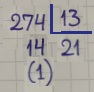
\includegraphics{divisionenpapel.jpg}
    \caption{Típica división escolar}
    \par\small Fuente: Elaboración propia
\end{figure}

El denominado Algoritmo de la División nos dice que tanto el cociente como el residuo son únicos.
\begin{enunciado}[Algoritmo de la División]\label{enun:algDivision}
\[\forall a,b \in \Z \text{ con } b \neq 0, 
\exists! q,r \in \Z \text{ tales  que }
a = q \cdot b + r \text{ donde } 0 \leq r < |b|\]
\end{enunciado}

\begin{proof}
Consideremos la progresión aritmética siguiente ($|b|$ es
la diferencia de la progresión):
\[ \ldots, a-3b, a-2b, a-1b, a+0b, a+1b, a+2b, a+3b, \ldots \]
De esta progresión seleccione el miembro \underline{no negativo menor} y denótelo como $r$. 
Siempre se puede expresar $r$ como $a-qb$ para algún $q \in \Z$.

En efecto, dado que todos los términos de la progresión son de la forma $a+kb$ con $k \in \Z$, siempre existe un entero $q$ tal que $r = a-qb$, basta tomar $q = -k$. 

Dado que se elige el miembro no negativo menor, es claro que: 
\begin{enumerate}[label=(\roman*)]
    \item $0 \leq r$.
    \item Mostraremos ahora que $r < |b|$, es decir, $r-|b| < 0$. 
\end{enumerate}

En efecto, supongamos que:
\begin{equation}
\label{eq35}
    r \geq |b|, \text{ es decir }, r -|b| \geq 0
\end{equation}
Como $r = a-qb$, entonces (\ref{eq35})  no es otra cosa que: $a-qb -|b| \geq 0$. 
O sea, por el valor absoluto, $a-qb - b \geq 0$ o $a-qb + b \geq 0$, que es lo mismo que:
\begin{equation}
    \label{eq41}
    a-(q+1)b \geq 0 \text{ o } a-(q-1)b \geq 0
\end{equation}
Pero entonces, no sólo $r - |b| \geq 0$, sino que, por la forma como se expresa esta desigualdad en (\ref{eq41}), $r - |b|$ es miembro de la progresión. 

Dado que $b \neq 0$, resulta que: 
\[|b| > 0 \qquad // \cdot(-1) \]
\[ -|b| < \, 0 \quad // +r \ \]
\[ r-|b| < \, r \]
Resumiendo: $r - |b| \geq 0$; $r - |b|$ miembro de la progresión; $r - |b| < r$. 

Ello contradice la elección de $r$ como el menor miembro no negativo.
Esta contradicción invalida nuestro supuesto, confirmando que
$r < |b|$. 

Falta probar la unicidad de $q,r$: 
Suponga que hay otro $r'$ tal que $r' = a-q'b$ con $0 \leq r' < |b|$. 
Es decir, $a = q'b + r'$ tal que $0 \leq r' < |b|$. 
Luego: $0 = a - a = qb + r - (q'b + r') = (q-q')b + (r-r')$.\\
Es decir: 
\begin{equation}
    \label{eq62}
    (r-r') = (q'-q)b
\end{equation}
Como $r'$ es un entero diferente de $r$, su diferencia no es cero, y por tanto, es claro que $q' \neq q$. Es decir $(q'-q) \neq 0$.
Luego (al trabajar en los enteros), el valor de $(q' - q)$ puede ser: 1 o -1 o 2 o -2 etc.
Es decir: $|q' - q| \geq 1$. Y como $b \neq 0$, de (\ref{eq62}) se deduce que: 
\begin{equation}
    \label{eq69}
    |r - r'| \geq |b|
\end{equation}
Pero ello contradice el hecho de que $0 \leq r < |b|$ y $0 \leq r' < |b|$. 

En efecto, tenemos: 
\[r < |b| \]  
\[r' \geq 0 \quad // \cdot(-1) \]
\[-r' \leq 0 \]
Luego:
$(r-r') < |b|$.
De modo análogo, tenemos: 
\[r \geq 0 \]
\[r' < |b| \quad // \cdot(-1)\]
\[ -r' > -|b| \]
Luego:
$(r-r') > -|b|$

Resumiendo: $(r-r') < |b|$ y $(r-r') > -|b|$\\
Recordemos que, por definición de valor absoluto, tenemos dos casos: 

Primer caso: $|r-r'| = r-r'$ cuando $r-r' \geq 0$. 
Como $(r-r') < |b|$, resulta que $|r-r'| < |b|$. 

Segundo caso: $|r-r'| = -(r-r')$ cuando $r-r' < 0$. Dado que 
\[(r-r') > -|b| \quad // \cdot(-1)\]
\[-(r-r') < |b| \]

Resultando que: $|r-r'| < |b|$. \\
En ambos casos: $|r-r'| < |b|$.

Así pues tenemos por un lado que $|r-r'| < |b|$  y por otro lado que (\ref{eq69}) $|r - r'| \geq |b|$. 

Dicha contradicción desahucia nuestro supuesto y confirma la unicidad de $q,r$. 
\end{proof}

\begin{itemize}
    \item $a,b$ se llaman respectivamente dividendo y divisor.
    \item $q,r$ se llaman respectivamente cociente y residuo de la división de $a$ entre $b$
\end{itemize}

Note que, dados $a,b$ la demostración ofrece un algoritmo para hallar los números $q,r$ a través de la progresión aritmética, el miembro no negativo menor y la forma de $r = a-qb$.

\begin{ejemplo}
Dados el dividendo $a = 5$ y el divisor $b = -2$, el cociente y el residuo son $q = -2$ y $r = 1$. \\
En efecto, la progresión es: \[
\ldots, 5-2\cdot (-2), 5-1\cdot (-2), 5+0\cdot (-2), 5+1\cdot (-2), 5+2\cdot (-2), 5+3\cdot (-2), \ldots \]
Es decir: \[
 \ldots, \qquad 9 \qquad, \qquad 7 \quad \quad, \qquad 5 \qquad, \qquad 3 \qquad, \qquad 1 \qquad, \qquad -1 \qquad,\ldots \]
El no negativo menor es $r = 1$. 
Todos los términos de la progresión son de la forma $a+kb$ con $k \in Z$, en el ejemplo el residuo 1 corresponde a $5+2\cdot (-2)$ con $k =  2$. Dado que en la demostración trabajamos con $r = a-qb$, tomamos $q = -k$, de donde se tiene que $q = -2$.
\end{ejemplo}

\section{Definiciones básicas}

\subsection{Divisibilidad}
\begin{definicion}[Divisibilidad]\label{def:divisibilidad}
Sean $a, b \in \Z$ con $b \neq 0$. 
Diremos que $b$ divide $a$ (o que $b$ es divisor o factor de $a$, o que $a$ es un múltiplo de $b$), denotado $b \mid a$, si $\exists q \in \Z$ tal que $a = qb$. Si $b<a$ se dice que es un divisor propio.
\end{definicion}

En relación con el algoritmo de la división, es evidente que $r = 0$ si y sólo si $b \mid a$. \\
Que $b$ no sea divisor de $a$ ($b$ no divide $a$) se denota así: $b \nmid a$.

\begin{ejemplo}
Con $a = 21$ y $b = 7$, tenemos que $b \mid a$ pues $21 = 3 \cdot 7$, con $q = 3$ y $r = 0$.
\end{ejemplo}

\begin{ejemplo}
Con $a = 20$ y $b = 6$, tenemos que $b \nmid a$ pues $20 = 3 \cdot 6 + 2$, con $q = 3$ y $r = 2$, es decir, $r \neq 0$.
\end{ejemplo}

\subsection{Máximo común divisor (mcd) y mínimo común múltiplo (mcm)}
\begin{definicion}[Divisor común]\label{def:divComun}
Dados $a,c \in \Z$, diremos que $d \in \Z$ es un divisor común de $a$ y $c$ si $d \mid a$ y $d \mid c$.
\end{definicion}

\begin{definicion}[mcd]\label{def:mcd}
Dados $a,c \in \Z$, no nulos ambos, diremos que $d \in \Z^{+}$ es el máximo cómún divisor de $a$ y $c$ si $d$ es el positivo mayor de los divisores comunes de $a$ y $c$. 
Se denota así: $mcd(a,c)$.
\end{definicion}

\begin{ejemplo}
El número 4 es divisor común de 24 y 36 pues $4 \mid 24$ \; y \; $4 \mid 36$.
\end{ejemplo}

\begin{ejemplo}
El número 12 es el máximo común divisor de 24 y 36, es decir, mcd(24,36) = 12, pues $12 \mid 24$ \; y \; $12 \mid 36$ y no hay otro divisor común positivo mayor a 12.
\end{ejemplo}

\begin{definicion}[mcm]\label{def:mcd}
El mcm (mínimo común múltiplo) de dos o más enteros $a_1, \ldots, a_r$ es el número positivo más pequeño que es múltiplo de todos ellos a la vez.  \\
Se denota así: $mcm(a_1, \ldots, a_r)$.
\end{definicion}

\begin{ejemplo}
El número $240$ es múltiplo común de $30, 40$ y $60$ pero no es el mínimo. \\
$mcm(30,40,60)=120$.
\end{ejemplo}

Tanto el $mcd$ como el $mcm$ son operaciones asociativas.

\subsection{Números primos y coprimos}

\begin{definicion}[Número primo]\label{def:numPrimo}
Un entero positivo $p > 1$ se llama número primo si sus únicos divisores positivos son 1 y $p$.
\end{definicion}

Un entero $n > 1$ no primo, se dice que es compuesto. 
El número 1 no es ni primo ni compuesto.

\begin{ejemplo}
Los números 3 y 5 son número primos pues sólo tienen a 1 y a sí mismos como divisores positivos.
\end{ejemplo}

\begin{ejemplo}
El número 6 es compuesto pues además de tener a 1 y 6 como divisores positivos, también $2 \mid 6$ \; y \; $3 \mid 6$.
\end{ejemplo}

\begin{definicion}[Números coprimos] \label{def:numCoprimo}
Dados $a,c \in \Z$, diremos que son coprimos (o primos entre sí o primos relativos) si $mcd(a,c) = 1$.
\end{definicion}

\begin{ejemplo}
Los números 4 y 9 son coprimos pues los divisores de 4 son 1, 2 y 4, los divisores de 9 son 1,3 y 9, de modo que mcd(4,9) = 1.
\end{ejemplo}

\subsection{Factor primo y factorización}
\begin{definicion}[Factor primo]\label{def:factorPprimo}
$\forall n \in \Z \; \ con \ n > 1, \text{un número primo} \ p$ se llama 
factor primo de $n$ si $p \mid n$.
\end{definicion}

\begin{definicion}[Factorización prima y multiplicidad]\label{def:factorizacion}
$\forall n \in \Z$ \; con $n > 1$, llamaremos factorización prima de $n$ a una expresión de la forma $n = p_1^{a_1} p_2^{a_2} \cdots p_k^{a_k}$, donde cada $p_i$ es un factor primo distinto y cada $a_i \in \N^{+}$.  El exponente $a_i$ se llama multiplicidad del factor primo $p_i$ en $n$, y representa la mayor potencia de $p_i$ tal que $p^{a_i} \mid n$.
\end{definicion}

Es usual denominar factorización al proceso de búsqueda de todos los factores primos junto a su multiplicidad.

\begin{ejemplo}
$n = 20$ tiene como factores primos a 2 y 5, pues $2|20$ y $5|20$. \\
La multiplicidad del factor primo 2 es 2, pues es el máximo exponente tal que $2^{2} \mid 20$. \\
La multiplicidad del factor primo 5 es 1, pues es el máximo exponente tal que $5^{1} \mid 20$ \\
La factorización de $20$ se expresa así: $20 = 2^{2} \cdot 5^{1} = 2^{2}5^{1}$.
\end{ejemplo}

\section{Propiedades de las definiciones básicas}
\subsection{Divisibilidad}
\begin{enunciado}[Propiedades de la divisibilidad]\label{enun:propDivisibilidad}\leavevmode\par
\begin{enumerate}[label=\roman*)]
\item Si $b \mid a$ \; y \; $b \mid c$ entonces $\forall x,y \in \Z$ \; $b \mid (ax + cy)$
\item Si $b \mid a$ \; y \; $a,b > 0$ entonces $b \leq a$
\item Si $b \mid a$ entonces $\forall x \in \Z$ \; $b \mid ax$
\item Si $a < b$ \; y \; $a,b > 0$ entonces $b \nmid a$
\item Si $c \mid b$ \; y \; $b \mid a$ entonces $c \mid a$
\item Si $b \mid (a+c)$ \; y \; $b \mid c$ entonces $b \mid a$
\end{enumerate}
\end{enunciado}

\begin{proof} Empecemos.
\begin{enumerate}[label=\roman*)]
\item Como $b \mid a$ \; y \; $b \mid c$ entonces $\exists q,q' \in \Z$ tales que $a = qb$ y $c = q'b$.
Luego: $ax + cy = qbx + q'by = (qx + q'y)b$. \\
Como $q,q',x,y \in \Z$, es obvio que $(qx + q'y) \in \Z$, entonces $b \mid (ax + cy)$. 
\item Como $b \mid a$ entonces $a = qb$. \\
Como $a,b > 0$, se deduce que $q > 0$, es decir, $q \geq 1$. \\
Por lo tanto: $qb \geq b$, es decir, $a \geq b$.  \label{inciso2}
\item Como $b \mid a$ entonces $a = qb$. \\
Luego: $ax = qbx = (qx)b$. \\
De lo cual, se desprende que $b \mid ax$. \\
\item Sabemos que $a,b >0$. \\
Supongamos que $b \mid a$. \\
Por el inciso \ref{inciso2} entonces $b \leq a$. Pero ello contradice $a<b$. \\
Por lo tanto, nuestro supuesto es errado y el enunciado se confirma. 
\item Como $c \mid b$ \; y \; $b \mid a$, resulta que $b = qc$ \; y \; $a = q'b$. Luego: \\
$a = q'b = q'qc = (q'q)c$. \\
De donde se deduce que $c \mid a$. 
\item Como $b \mid (a+c)$ \; y \; $b \mid c$ entonces $(a+c)=qb$ \; y \; $c=q'b$. Luego: \\
$(a+q'b) = qb$. Es decir: \\
$a = qb-q'b = (q-q')b$. \\
De donde se deduce que $b \mid a$.
\end{enumerate}
\end{proof}

\begin{ejemplo} Los incisos corresponden a los del enunciado. 
\begin{enumerate}[label=\roman*)]
\item Como $3 \mid 6$ \; y \; $3 \mid 15$ entonces $3 \mid (6 \cdot 3 + 15 \cdot (-7))$, es decir, $3 \mid -87$.
\item Como $2 \mid 4$ entonces $2 \leq 4$. 
Nótese que $-2 \mid -8$ pues $-8 = 4(-2)$. ¡Pero $-2 > -8$! \\
Ello no contradice el resultado pues, en este último caso, no es cierto que $a,b > 0$. 
\item Como $3 \mid 15$ entonces $3 \mid (15 \cdot (-1))$, es decir $3 \mid -15$.
Como $6 < 12$ \; y \; $6,12 > 0$ entonces $12 \nmid 6$.
\item Como $7 \mid 14$ \; y \; $14 \mid 28$ entonces $7 \mid 28$. 
\item Como $7 \mid (21+14)$ \; y \; $7 \mid 14$ entonces $7 \mid 21$.
\end{enumerate} \end{ejemplo}

\subsection{Máximo común divisor}
\begin{enunciado}[Propiedades del mcd]\label{enun:propMcd}\leavevmode\par
\begin{enumerate}[label=\roman*)]
\item Identidad de Bezout. Si $d = mcd(a,c)$ entonces  $\exists x,y \in \Z$ tales que $d = ax + cy$  
\item $mcd(-a,b) = mcd(a,b) = mcd(a,-b) = mcd(-a,-b) = mcd(|a|,|b|)$ 
\item $mcd(a,b) = mcd(b,a)$
\item Si $a,b \neq 0$ y $d = mcd(a,b)$ entonces $d \leq |a|$ y $d \leq |b|$
\item Para $a \neq 0, mcd(a,a) = |a|$
\item Para $b \neq 0, mcd(0,b) = mcd(b,0) = |b|$
\item Si $a,b > 0$ entonces $mcd(a,b) = mcd(b,r)$ \; \; ($r$ es el residuo de la división de a entre b) 
\item Lema de Euclides. Si $a \mid bc$ y $mcd(a,b) = 1$ entonces $a \mid c$
\item Una ecuación del tipo $ax + by = n$, se denomina ecuación diofántica. \\
La ecuación diofántica $ax + by = n$ tiene soluciones enteras
si y sólo si $mcd(a,b) \mid n$ 
\item Si $x_0,y_0$ es solución de la ecuación diofántica $ax + by = n$ entonces $\forall i$ tal que $i > 0$ $x' = x_0 + i \cdot \frac{b}{d}, y' = y_0 - i \cdot \frac{a}{d}$ también es solución
\end{enumerate} \end{enunciado}

\begin{proof} Empecemos. 
\begin{enumerate}[label=\roman*)]
\item Sea $S = \{ax + cy\}$ donde $x,y \in \Z$. \\
Escójanse $x_0,y_0$ tales que $b = ax_0 + cy_0$ sea el elemento positivo menor de S. \\
Por el algoritmo de la división,
\begin{equation} \label{eq273}
    \exists! q, r \in \mathbb{Z} \text{ tales que } a = qb + r, \text{ con } 0 \leq r < |b|
\end{equation}

Luego, $r = a-qb = a - q(ax_0 + cy_0) = a - qax_0 - qcy_0 = a(1 - qx_0) + c(-qy_0)$. 

Como $1,q,x_0,y_0 \in \Z$ es obvio que $(1 - qx_0), (-qy_0) \in \Z$. 

Por lo tanto, $r \in S$. 

Como $0 \leq r < |b|$ , es imposible que $0 < r$, pues el menor elemento positivo de S es b. 

Sólo queda la posibilidad $r = 0$. Y en ese caso, de (\ref{eq273}): $b \mid a$. 

Un razonamiento prácticamente idéntico 
($\exists! q,r \in \Z$ tales que $c = qb + r$) nos muestra que: $b \mid c$. 

Como $d$ es el máximo común divisor de $a$ y $c$, por definición: $d \mid a$ \, y \, $d \mid c$. 

Luego, por el Enunciado~\ref{enun:propDivisibilidad}.\roman{enumi}: 
$\forall x,y \in \Z \; \, d \mid (ax + cy)$. \\
En particular, $d \mid (ax_0 + cy_0)$. \\
Es decir: $d \mid b$, pues $b = ax_0 + cy_0$ \\
\setcounter{enumi}{2}
Por el Enunciado~\ref{enun:propDivisibilidad}.\roman{enumi}: $d \leq b$. \\
Por definición de máximo común divisor, d es positivo. \\
Por la forma de seleccionarlo, b es positivo. \\
Resumiendo: $b \mid a$ y $b \mid c$, $d \leq b$, $d$ es el máximo común divisor. \\
No nos queda sino concluir que $b = d$. \\
Es decir, $d = mcd(a,c) = ax_0 + cy_0$. Lo que prueba el enunciado. 
\setcounter{enumi}{1}
\item Mostraremos que $mcd(-a,b) = mcd(a,b)$ \\
Sea $d  =  mcd(-a,b)$. Es decir, $d \mid -a$ \, y \, $d \mid b$ (es el divisor común positivo más grande). \\
\setcounter{enumi}{3}
Por el Enunciado~\ref{enun:propDivisibilidad}.\roman{enumi}: $d \mid (-ax)$, tomemos $x = -1$, es decir, $d \mid a$.
Luego: $d \mid a$ y $d \mid b$. \\
No hay otro divisor positivo más grande. En efecto: \\
Supongamos que $d' \mid a$ \, y \, $d' \mid b$ con $d' > d$. De nuevo por el Enunciado~\ref{enun:propDivisibilidad}.\roman{enumi} con $x = -1$:
$d' \mid -a$ y $d' \mid b$, con $d' > d$, lo que contradice que $d  =  mcd(-a,b)$. \\
Por lo tanto: $d  =  mcd(a,b)$. \\
Los otros casos se prueban idénticamente, junto a la definición de valor absoluto en el último caso: 

$|a| = 
\begin{cases}
  a, & \text{si } a \geq 0, \\
  -a, & \text{si } a < 0.
\end{cases}$ 
\setcounter{enumi}{2}
\item Trivial. Por definición $d = mcd(a,b)$ es el divisor común positivo más grande de a y b. Luego, d es el positivo más grande tal que $d \mid a$ \, y \, $d \mid b$. Por tanto, d es el positivo más grande tal que $d \mid b$ \, y \, $d \mid a$.\\
Es decir, por definición, $d = mcd(b,a)$. 
\item  \setcounter{enumi}{2}
Por el inciso \roman{enumi}: $d = mcd(a,b) = mcd(|a|,|b|)$, es decir, $d \mid |a|$ \, y \, $d \mid |b|$. También $d > 0$ por definición. \\
Como $a,b \neq 0$: $|a| > 0$ \, y \, $|b| > 0$. Por el Enunciado~\ref{enun:propDivisibilidad}.\roman{enumi}: $d \leq |a|$ \,  y \, $d \leq |b|$. 
\setcounter{enumi}{4}
\item  
Sea $d = mcd(a,a)$. Por el inciso \roman{enumi}: $d \leq |a|$. \\
$|a|$ es divisor de $a$ pues $a = q|a|$, con $q = 1$ o $q = -1$. \\
Y como d es el máximo divisor, se concluye que $d = |a|$. 
\item \setcounter{enumi}{3} 
Por el inciso \roman{enumi}: Basta probar que para $b \neq 0, mcd(0,b) = |b|$. \\
\setcounter{enumi}{2}
Por el inciso \roman{enumi}: Es lo mismo probar que para $b \neq 0, mcd(0,|b|) = |b|$. \\
$|b|$ es divisor de $0$ pues: $0 = q|b|$ (con $q = 0$). \\
$|b|$ es divisor de $|b|$ pues: $|b| = q|b|$ (con $q = 1$). \\
Es decir, $|b|$ es divisor común de 0 y $|b|$. \\
No hay otro divisor común de 0 y $|b|$ más grande. En efecto:\\
Supongamos que lo hay. 

Sea d ese divisor común de 0 y $|b|$, con:
\begin{equation}
\label{eq343}
d > |b| 
\end{equation}


Como $b \neq 0: |b| > 0$ y por lo tanto $d > 0$. \\
Como $d$ es divisor de $|b|$ existe un $q$ talque
\begin{equation}
\label{eq351}
    |b| = qd
\end{equation}

Para que la última igualdad se mantenga (\ref{eq351}), dado que $|b|$,$d > 0$, se deduce que $q > 0$, es decir: 
\[
 q \geq 1 \quad // \cdot d
\]
\[
qd \geq d
\]
Luego, aplicando (\ref{eq351}): 
$|b| \geq d$. Lo que contradice la ecuación (\ref{eq343}). 

Así, nuestro supuesto es errado y $mcd(0,b) = |b|$. 
\setcounter{enumi}{6}
\item Por el Enunciado~\ref{enun:algDivision}: $a = qb + r$. Es decir: $r = a - qb$. \\
Sea $d = mcd(a,b)$ (es obvio que $d \mid a$ y $d \mid b$). \\
\setcounter{enumi}{1}
Por el Enunciado~\ref{enun:propDivisibilidad}.\roman{enumi}: $d \mid (a - qb)$. (con $x = 1, y = -q$). \\ Es decir, $d \mid r$ (y $d \mid b$). \\
No hay otro $d' > d$ tal que $d' \mid b$ y $d' \mid r$. En efecto: \\
Suponiendo que lo haya, por el mismo Enunciado~\ref{enun:propDivisibilidad}.\roman{enumi}: \\
$d' \mid (qb + r)$. \\
Es decir, $d' \mid a$, y como $d' \mid b$, se contradice el hecho de que $d = mcd(a,b)$. \\
Luego el supuesto es erróneo y $d = mcd(b,r) = mcd(a,b)$.
\setcounter{enumi}{7}
\item \setcounter{enumi}{1}
Como $mcd(a,b) = 1$, por el inciso \roman{enumi}: $1 = ax + by$. Luego: \\
$c = axc + byc$, es decir: $ c = acx + bcy$ \\
Es evidente que $a \mid ac$. \\
Por hipótesis sabemos que $a \mid (bc)$. Luego, por el Enunciado~\ref{enun:propDivisibilidad}.\roman{enumi}: \\
$ a \mid acx + bcy$. De donde se deduce que $a \mid c$.
\setcounter{enumi}{8}
\item Demostraremos el resultado, probando cada sentido de la doble implicación: \\
Sea $d=mcd(a,b)$.
\begin{enumerate}
\item Si la ecuación diofántica $a \cdot x+b \cdot y=n$ tiene soluciones enteras\\
entonces $mcd(a,b) \mid n$ :\\
Como $d=mcd(a,b)$ entonces: $d \mid a$ y $d \mid b$.\\
Entonces por el Enunciado~\ref{enun:propDivisibilidad}.i: $\forall x,y \in \Z: d \mid(a \cdot x+b \cdot y)$.\\
Por hipótesis existen $x_{0}, y_{0} \in \Z$ tales que $a \cdot x_{0}+b \cdot y_{0}=n$,\\
Por lo tanto: $d \mid n$.
\item Si $mcd(a, b) \mid n$ entonces\\
la ecuación diofántica $a \cdot x+b \cdot y=n$ tiene soluciones enteras:\\
Como $d=mcd(a,b)$, (por el inciso i): $\exists x_{0}, y_{0} \in \Z$ tales que $d=a \cdot x_{0}+b \cdot y_{0}$\\
Por hipótesis: $d \mid n$. Es decir: $\frac{n}{d} \in \Z$\\
Por lo tanto: $\frac{n}{d} \cdot x_{0} \in \Z, \frac{n}{d} \cdot y_{0} \in \Z$\\
Además ambos enteros solucionan la ecuación diofántica pues:\\
$a \cdot \frac{n}{d} \cdot x_{0}+b \cdot \frac{n}{d} \cdot y_{0}=\frac{n}{d} \cdot (a \cdot x_{0}+b \cdot y_{0})=\frac{n}{d} \cdot d=n$
\end{enumerate}
\setcounter{enumi}{9}
\item $a \cdot x'+b \cdot y'=a \cdot (x_{0}+i \cdot \frac{b}{d})+b \cdot(y_{0}-i \cdot \frac{a}{d})=a \cdot x_{0}+i \cdot a \cdot \frac{b}{d}+b \cdot y_{0}-i \cdot b \cdot \frac{a}{d}=a \cdot x_{0}+b \cdot y_{0}=n$
\end{enumerate}
\end{proof}

\begin{ejemplo} Los incisos corresponden a los del enunciado.
\begin{enumerate}[label=\roman*)]
\item $d = mcd(28,19) = 1$ \\
$\hspace*{0.8em}1 = 28(-2) + 19(3)$   con $x = -2, \, y = 3$. 
\item $mcd(12,18) = mcd(-12,18) = mcd(12,-18) = mcd(-12,-18) = 6$. 
\item $mcd(15,9) = mcd(9,15) = 3$. 
\item Con $a = -14, \, b = 35, mcd(-14,35) = 7, 7 \leq |-14| \, y \, 7 \leq |35|$. 
\item Con $a = -5, \, mcd(-5,-5) = 5 = |-5|$. 
\item Con $b = -12, \, mcd(-12,0) = mcd(-12,0) = 12 = |-12|$. 
\item Con $a = 56, \, b = 15, 56 = 15 \cdot 3 + 11$, donde $r = 11$. \\
$\hspace*{1.6em}mcd(56,15) = mcd(15,11) = 1$
\item Con $a = 5, \, b = 3, \, c = 10, bc = 30, 5 \mid 30, mcd(5,3) = 1, 5 \mid 10$.
\item  $4x + 6y = 10$ tiene solución pues $mcd(4,6) = 2$ y $2 \mid 10$; $x_0=1, y_0=1$ solucionan esta ecuación diofántica.
\item Dada la solución $x_0=1, y_0=1$ para $4x + 6y = 10$, con $i=1$, $x'=1+1 \cdot \frac{6}{2}=4, y'=1-1 \cdot \frac{4}{2}=-1$ también es solución.
\end{enumerate}
\end{ejemplo}

\subsection{Divisores primos y teorema fundamental de la aritmética}
\begin{enunciado}[Propiedades de un divisor primo]\label{enun:propDivprim}
\leavevmode\par
\begin{enumerate}[label=\roman*)]
\item Sea $p$ primo. $\forall a \in \Z$ \, se tiene $p \mid a$ \, o \, $mcd(a,p) = 1$ 
\item Sea $p$ primo. $\forall a,b \in \Z$ \; Si $p \mid ab$ entonces $p \mid a$  \, o  \, $p \mid b$
\item Generalización del Lema de Euclides. Sea $p$ primo. $\forall a_1, \ldots, a_k \in \Z$  \; Si $p \mid (a_1 \cdot \ldots \cdot a_k)$ entonces $\exists i$, con $1 \leq i \leq k$, tal que $p \mid a_i$
\end{enumerate}
\end{enunciado}

\begin{proof} Empecemos.
\begin{enumerate}[label=\roman*)]
\item Sea $d = mcd(a,p)$. \\
Dado que $p$ es primo sus únicos divisores son $1$ y $p$, luego $d = 1$ o $d = p$. \\
Si $d = 1$, entonces $mcd(a,p) = 1$. \\
Si $d = p$, como $d \mid a$ entonces $p \mid a$. \\
En ambos casos, se cumple $p \mid a$ \, o \, $mcd(a,p) = 1$. 
\item Si $p \mid a$ el resultado es cierto inmediatamente. \\
Supongamos que $p \nmid a$. \\
Como $p$ es primo, sus únicos divisores son $1$ y $p$, de modo que el único divisor común positivo entre $a$ y $p$ es $1$ (el otro candidato es $p$, pero al no ser divisor de a, se descarta). Luego, $mcd(a,p) = 1$. \\ 
Por el Enunciado~\ref{enun:propMcd}, concretamente el Lema de Euclides, $p \mid b$. \\
Ello prueba que o bien $p \mid a$ \, o \, $p \mid b$. 
\item Como $p \mid (a_1 \cdot \ldots \cdot a_k)$ es obvio que $p \mid (a_1 \cdot (a_2 \cdot \ldots \cdot a_k))$. \\
\setcounter{enumi}{2}
Por el inciso \roman{enumi}: $p \mid a_1$ o $p \mid (a_2 \cdot \ldots \cdot a_k)$. \\
Si $p \mid a_1$ el resultado es cierto inmediatamente. \\
Si $p \mid (a_2 \cdot \ldots \cdot a_k)$ entonces $p \mid (a_2 \cdot (a_3 \cdot \ldots \cdot a_k))$. Etc. \\
Es un corolario del inciso \roman{enumi}.
\end{enumerate}
\end{proof}

\begin{ejemplo} Los incisos corresponden a los del enunciado. \\
\begin{enumerate}[label=\roman*)]
\item Con $p = 7$, \, $a = 14, 7 \mid 14$. Se cumple que $p \mid a$.\\
\hspace*{1em} Con $p = 7, \, a = 15, \, mcd(7,15) = 1$. Se cumple que $mcd(a,p) = 1$.
\item Con $p = 5, a = 10, b = 3, 10 \cdot 3 = 30, 5 \mid 30, 5 \mid 10$. Se cumple que $p \mid a$. \\
\hspace*{1em} Con $p = 3, a = 7, b = 12, 7 \cdot 12 = 84, 3 \mid 84, 3 \mid 12$. Se cumple que $p \mid b$.
\item Con $p = 11, a_1 = 4, a_2 = 11, a_3 = 9, a_4 = 5, a_5 = 2, 4 \cdot 11 \cdot 9 \cdot 5 \cdot 2 = 3960, 11 \mid 3960$ \\  \hspace*{1.2em} $\exists i, i = 2$, tal que $11 \mid a_2$. 
\end{enumerate}
\end{ejemplo}

\begin{enunciado}[Teorema fundamental de la aritmética (factorización única)]\label{enun:teorFundAritm}
$\forall n \in \Z$ \; con $n > 1$, (salvo el orden de los factores)  existe una única factorización prima de $n$, es decir, una única expresión de la forma $n = p_1^{a_1} p_2^{a_2} \cdots p_k^{a_k}$.
\end{enunciado}

\begin{proof} Si $n$ es primo, por sí solo se considera como el producto de un único factor. \\ 
En otro caso, designemos por $p_1$ a su divisor primo menor, luego (por definición de divisor): $n = p_1n_1$. 
\begin{itemize}
    \item Si $n_1 > 1$, designemos por $p_2$ a su divisor primo menor, luego:  $n_1= p_2 n_2$.
    \item Si $n_2 > 1$, designemos por $p_3$ a su divisor primo menor, luego:  $n_2 = p_3 n_3$. 
    \item Hasta que obtengamos un $n_r = 1$, de manera que $n_{r-1} = p_r$.
\end{itemize}

En efecto, este proceso de escribir n como el producto de sus factores primos debe terminar porque los factores son menores que n y además cada factor primo es un entero mayor que $1$. 

Reemplazando $n_1$ en la primera igualdad por $p_2 n_2$, y luego reemplazando $n_2$ en el resultado, y así sucesivamente, $n$ puede expresarse como el producto de estos factores primos hallados como hemos indicado: $n = p_1 p_2 \cdots p_{r-1} p_r$ 
Y como los factores primos no son necesariamente distintos podemos escribir: 

$n = p_1^{a_1} p_2^{a_2} \cdots p_k^{a_k}$, donde $p_1, p_2, \cdots, p_k$ son primos distintos y $a_1, a_2, \cdots, a_k$ son positivos. 

Es el turno de la \underline{unicidad}: 

Supongamos que hay enteros positivos con más de una factorización. Sea $n$ (con $n > 1$) el menor de ellos. 

Nótese que estamos llamando factorización (y no factorización prima) a la expresión que contiene factores primos duplicados, todavía sin unificarlos a través de los exponentes $a_i$.

Como para $n$ hay otra factorización, sea dicha factorización alterna la siguiente: 
\begin{equation}
\label{eq1}
n = q_1 q_2 \cdots q_{s-1} q_s
\end{equation}
Luego: $p_1 p_2 \cdots p_{r-1} p_r = q_1 q_2 \cdots q_{s-1} q_s$\\ 
Es claro que $q_1 \mid q_1 q_2 \cdots q_{s-1} q_s$. Luego: \\ 
$q_1 \mid p_1 p_2 \cdots p_{r-1} p_r$ (es decir: $q_1 \mid n$). \\
\setcounter{enumi}{3}
Por el Enunciado~\ref{enun:propDivprim}.\roman{enumi}: $q_1$ es divisor de al menos uno de los $p_i$. \\ 
Podemos suponer (reordenando los factores primos si es necesario) que $q_1 \mid p_1$. \\ 
Pero $p_1$ y $q_1$ son primos, luego, necesariamente: $p_1 = q_1$.    (luego:  $p_1 \mid n$) \\ 
Simplificando (\ref{eq1}) por $p_1 = q_1$ tenemos que: 
\begin{equation}
\label{eq481}
m = n/p_1 = 1 p_2 \cdots p_r-1 p_r =  q_2 \cdots q_{s-1}  q_s
\end{equation}
Como $p_1 \mid n$, entonces $m$ es un entero positivo. Además: $m < n$. \\ 
Pero entonces, (\ref{eq481}) nos muestra que $m$ tiene más de una factorización. \\ 
Lo que contradice que $n$ sea el menor de los enteros positivos con más de una factorización. \\ 
De ahí que nuestro supuesto es erróneo y la factorización es única.
\end{proof}

\begin{ejemplo} Trabajemos con $n = 252$. \\
Factorización (como en la demostración): \\
El menor primo que divide a 252 es 2. \\
$252 = 2 \cdot 126$. \\
El menor primo que divide a 126 es 2. $126 = 2 \cdot 63$. Luego: \\
$252 = 2 \cdot 2 \cdot 63$. \\
El menor primo que divide a 63 es 3. $63 = 3 \cdot 21$. Luego: \\
$252 = 2 \cdot 2 \cdot 3 \cdot 21$. \\
El menor primo que divide a 21 es 3. $21 = 3 \cdot 7$. Luego: \\
$252 = 2 \cdot 2 \cdot 3 \cdot 3 \cdot 7$. \\
El menor primo que divide a 7 es 7. $7 = 7 \cdot 1$. \\
Hemos obtenido un $n_r = 1$, de manera que $n_{r-1} = p_r = 7$. Luego: \\
$n = p_1 p_2 \cdots p_{r-1} p_r$. Es decir: \\ 
$252 = 2 \cdot 2 \cdot 3 \cdot 3 \cdot 7$. \\ \\
Factorización prima de $n = 252$, con  $a_1 = 2, a_2 = 2, a_3 = a_k = 1$ : \\
$252 = 2^{2} \cdot 3^{2} \cdot 7^{1} = 2^{2} \cdot 3^{2} \cdot 7 $.
\end{ejemplo}

\begin{enunciado}[Infinitud de primos]\label{enun:infPrim} Existen infinitos números primos.
\end{enunciado}

\begin{proof} Por reducción al absurdo. \\
Supongamos que sólo hay $n$ número primos. \\
Listémoslos en forma creciente así: $p_1, p_2, \cdots, p_n$. \\
Sea $N = p_1 p_2 \cdots p_{n-1} p_n + 1$. De donde, $N - p_1 p_2 \cdots p_{n-1} p_n = 1$. \\
Por el teorema fundamental de la aritmética, Enunciado~\ref{enun:teorFundAritm}, existe una factorización prima única de $N$. Es decir, $N$ es un producto de primos, llamemos $p_j$ a uno de ellos.  Otra forma de decirlo es que $N$ tiene al menos un divisor primo $p_j$. Es decir: $p_j \mid N$. \\
También es obvio que $p_j \mid p_1 p_2 \cdots p_n$. \\
\setcounter{enumi}{1}
Por el Enunciado~\ref{enun:propDivisibilidad}.\roman{enumi}: $p_j \mid (N - p_1 p_2 \cdots p_n)$, con $x = 1, y = -1$. Es decir: $p_j \mid 1$. \\
Ello implica que $p_j = 1$. Lo que contradice que $p_j$ es primo. \\
De ahí que nuestro supuesto es erróneo y no hay un número finito $n$ de números primos.
\end{proof}

\section{Estructuras modulares y congruencia}
La palabra módulo tiene varios significados en matemática (por ejemplo es un sinónimo de valor absoluto).
Nos interesan los siguientes dos: el primero relacionado con el residuo, en tanto operación, y el segundo relacionado con la relación de congruencia.

\subsection{Módulo como operación}
$a \bmod b = r$ \; ($r$ es el residuo de la división de $a$ entre $b$). \\

\begin{ejemplo} $19 \bmod 17 = 2$ pues en la división de $a$ entre $b$, con $a = 19, b = 17$, el residuo $r = 2$. \\ En efecto, $19 = 1 \cdot 17 + 2$
\end{ejemplo}

\subsection{Módulo como base de la (relación de) congruencia}
Sea $n \in \N$. Sean $a,b \in \Z$. \\
Se dice que $a$ es congruente con $b$ módulo $n$ (o también $a,b$ son congruentes módulo $n$), lo que se denota así: $a \equiv b \pmod n$ (o, a veces, así $a \equiv_n b$), si  $a,b$ dan el mismo residuo cuando se dividen entre $n$. \\
Es decir: $a \equiv b \pmod n$  \; si y sólo si \;  $r = r'$ \\
donde $a \bmod n = r$ \; y \; $b \bmod n = r'$.

\begin{ejemplo} $16 \equiv 30 \pmod {14}$, pues $16 \bmod 14 = 2 = 30 \bmod 14$.
\end{ejemplo}

$a \equiv_n b$ es una relación. \\
$n$ se denomina el módulo de la congruencia.

\subsection{Propiedades}
\begin{enunciado} [Caracterización de la congruencia mediante divisibilidad]\label{enun:congrViaDivisib} $a \equiv b \pmod n$ si y sólo si $n \mid (a - b)$.
\end{enunciado}

\begin{proof} Se hace en dos partes. \\
Si $a \equiv b \pmod n$ entonces $n \mid (a - b)$. \\
En efecto, como $a \equiv b \pmod n$ entonces  $a \bmod n = r$, $b \bmod n = r'$ y $r = r'$. Es decir, por el algoritmo de la división, Enunciado~\ref{enun:algDivision}: \\ 
$a = qn + r$ con $0 \leq r < n$ \\ 
$b = q'n + r'$ con $0 \leq r' < n$ \\ 
Y $r - r' =  0$. Por lo tanto, $a - b =  (q - q')n$, y en consecuencia: $n \mid (a-b)$. \\ \\
Si $n \mid (a - b)$ entonces $a \equiv b \pmod n$.\\
En efecto, por el algoritmo de la división, Enunciado~\ref{enun:algDivision}: \\ 
$a = qn + r$ con $0 \leq r < n$ \\ 
$b = q'n + r'$ con $0 \leq r' < n$ \\ 
Por lo tanto, 
\begin{equation}
    \label{eq561}
    a - b =  (q - q')n  +  (r - r') 
\end{equation}
¿Cuál es el valor más grande (cota superior) que puede tomar $(r - r')$? 
Se lo obtiene tomando el valor máximo para $r$, que es $n-1$, y el valor mínimo que puede tomar $r'$, que es 0, por tanto la cota superior es $r - r' = n - 1 - 0 = n - 1$.
Por tanto, $ r - r' < n$. \\
¿Cuál es el valor más pequeño (cota inferior) que puede tomar $(r - r')$? 
Se lo obtiene tomando el valor mínimo para $r$, que es $0$, y el valor máximo que puede tomar $r'$, que es $n-1$, por tanto la cota inferior es $r - r' = 0 - (n - 1) = - (n - 1)$.
Por tanto, $-n < r - r' $. \\
De ambos razonamiento se tiene que:  $-n < r - r' < n$ \\ 
Dado que $n \mid (a - b)$ y como $n \mid n$ entonces, \setcounter{enumi}{1} por el Enunciado~\ref{enun:propDivisibilidad}.\roman{enumi}, $n \mid ((a - b) - (q - q')n$, es decir por (\ref{eq561}):  $n \mid (r - r')$. \\ 
Como  $ -n < r - r' < n$, el único entero del tipo $(r - r')$ que sea divisible por (o múltiplo de) $n$ en ese rango es $0$, se deduce que $r - r' = 0$, de donde $r = r'$, por tanto: $a \equiv b \pmod n$.
\end{proof}

\begin{enunciado} [Equivalencia de $\equiv$]\label{enun:congrEquiv}\leavevmode\par
La relación $\equiv$ (relación de congruencia) es una relación de equivalencia
\end{enunciado}

\begin{proof}
Recordemos que para $n\geq 1$: \\
$a \equiv b \pmod n$ si y sólo si $a \, mod \, n = b \, mod \, n$ \\
Reflexividad: \\
Es evidente que $n \mid (a-a)$, pues $a-a = 0 = qn$ con $q=0$. \\
Luego, $a \equiv a \pmod n$. \\
Simetría: \\
\setcounter{enumi}{3}
Es evidente que si $n \mid (a-b)$ entonces $n \mid (b-a)$ por el Enunciado~\ref{enun:propDivisibilidad}.\roman{enumi} con $x=-1$. \\
Es decir, si $a \equiv b \pmod n$, entonces  $b \equiv a \pmod n$. \\
Transitividad: \\
\setcounter{enumi}{1}
Es evidente que si $n \mid(a-b)$ y $n \mid(b-c)$ entonces $n \mid [(a-b)+ (b-c)]$ por el Enunciado~\ref{enun:propDivisibilidad}.\roman{enumi}, es decir, $n \mid (a-c)$. \\
Es decir, si $a \equiv b \pmod n$ y $b \equiv c \pmod n$
entonces $a \equiv c \pmod n$. \\
Luego, $\Z$  queda particionado en clases de equivalencia.\\
$[a]_n = \{ b \in \Z / a \equiv b \pmod n\} = \{\dots, a - 2n, a - n, a, a + n, a + 2n, \dots \}$ \\
Cada clase corresponde a uno de los $n$ posibles restos $r = 0, 1, \dots , n-1$. \\
Es evidente que si $n=1$: $\forall a \in \Z $  $a \equiv 0 \pmod 1$, pues $a \, mod \, 1 = 0$. Luego: \\
$[a]_1= \Z$. \\
En adelante, supondremos que $n>1$.
\end{proof}

\begin{enunciado} [Algunas propiedades del módulo como operación, se supone $n >1$]\label{enun:propMod}\leavevmode\par
\begin{enumerate}[label=\roman*)]
\item Si $n > m \geq 0$ \, entonces \, $m \bmod n = m$  
\item $\forall m \in \Z \quad (m \bmod n) \bmod n = m \bmod n$ 
\item $(a+b) \bmod n = (a \bmod n + b \bmod n) \bmod n$
\item $ (a \cdot b) \bmod n = (a \bmod n \cdot b \bmod n) \bmod n$
\end{enumerate}
\end{enunciado}

\begin{proof} Empecemos:
\begin{enumerate}[label=\roman*)]
\item Por el Enunciado~\ref{enun:algDivision}, $m = qn + r = 0 \cdot n + m$ con $0 \leq m < |n|$, \\ donde $q = 0, r = m$ son únicos. \\
Por definición \, $m \bmod n = r$. \\
Luego, en este caso: $m \bmod n = m$. 
\item Sabemos que $m \bmod n = r$, con $0 \leq r < |n|$. \\ $|n| = n$ pues $n > 1$. Luego: \\
$(m \bmod n) \bmod n$ \\
\setcounter{enumi}{1}
$= r \bmod n$ \qquad por el inciso \roman{enumi}) con $r < n$\\
$= r$ \\
$= m \bmod n$. 
\setcounter{enumi}{2}
\item $(a + b) \bmod n = (a \bmod n + b \bmod n) \bmod n$  \\ 
por definición de congruencia, es lo mismo que:  \\ 
$(a+b) \equiv (a \bmod n + b \bmod n) \pmod n$ \\
Luego, por el Enunciado~\ref{enun:congrViaDivisib}, lo que debemos probar es:  \\ 
$n \mid (a+b)-(a \bmod n + b \bmod n)$ \\ 
Sean $a \bmod n = r_a, b \bmod n = r_b$.  \\ 
Por el algoritmo de la división, sabemos que: $a = qn + r_a, b = q'n + r_b$.  \\ 
Luego lo que debemos probar es:  \\ 
$n \mid (qn+r_a + q'n + r_b) - (r_a + r_b)$. \\ 
Pero entonces, lo que debemos probar es: $n \mid (q+q')n$  \\ 
Lo que es inmediato. 
\item Debemos probar que $(a \cdot b) \bmod n = (a \bmod n \cdot b \bmod n) \bmod n$  \\ 
Que es exactamente lo mismo (por definición de congruencia) que:  \\ 
$(a \cdot b) \equiv (a \bmod n \cdot b \bmod n) \pmod n$ \\
Que es exactamente lo mismo que, por el Enunciado~\ref{enun:congrViaDivisib}, que:  \\ 
$n \mid (a \cdot b) - (a \bmod n \cdot b \bmod n)$  \\ 
(como por el algoritmo de la división $a \bmod n = a - qn, b \bmod n = b - q'n$) \\
Ello es exactamente lo mismo que :  \\ 
$n \mid (a \cdot b) - ([a - qn] \cdot [b - q'n])$  \\ 
Que es exactamente lo mismo que:  \\ 
$n \mid (a \cdot b - [a \cdot b - aq'n - qnb + qnq'n])$  \\ 
Que es exactamente lo mismo que:  \\ 
$n \mid (a \cdot b - a \cdot b + aq'n + qnb - qnq'n)$  \\ 
Que es exactamente lo mismo que:  \\ 
$n \mid (aq' + qb - qnq')n$  \\ 
Lo que es inmediato.
\end{enumerate}
\end{proof}

\begin{enunciado} [Algunas propiedades de la congruencia]\label{enun:propCongru}\leavevmode\par
\begin{enumerate}[label=\roman*)]
\item $a+c \equiv b+c \pmod  m$ si y sólo si $a \equiv b \pmod  m$
\item $\forall c \in Z$ Si $a \equiv b \pmod  m$ entonces $a \cdot c \equiv b \cdot c \pmod  m$
\item Si $a \equiv b \pmod  m$ y $c \equiv d \pmod  m$ entonces $a+c \equiv b+d \pmod  m$
\item Si $a \equiv b \pmod  m$ y $c \equiv d \pmod  m$ entonces $a \cdot c \equiv b \cdot d \pmod  m$
\item Si $a \cdot n \equiv b \cdot n \pmod  m$ y $mcd(m, n)=1$ entonces $a \equiv b \pmod  m$
\item Si $a \equiv b \pmod  m$ entonces $b \equiv a \pmod  m$
\item $a \cdot x \equiv a \cdot y \pmod  m$ si y solo si $x \equiv y \pmod  {\frac{m}{mcd(a,m)}}$
\item Si $a \equiv b \cdot c \pmod  m$ \, y \, $c \equiv 1 \pmod  m$ entonces $a \equiv b \pmod  m$
\item Si $a \equiv b \pmod  m$ entonces $a^{n} \equiv b^{n} \pmod  m$
\item $a \equiv b \pmod  m$ si y sólo si $a \equiv [b \mod m] \pmod m$
\item Si  $a+b \equiv c \pmod m \,$ y $\, b \equiv 0 \pmod m$ entonces $a \equiv c \pmod m$ 
\end{enumerate}
\end{enunciado}

\begin{proof} Empecemos:
\begin{enumerate}[label=\roman*)]
\item $a+c \equiv b+c \pmod  m$ si y sólo si $m \mid (a+c-(b+c))$ (Enunciado~\ref{enun:congrViaDivisib}) \\
si y sólo si $m \mid (a-b)$  \quad\quad\quad (obvio)\\
si y sólo si $a \equiv b \pmod  m \quad$ (Enunciado~\ref{enun:congrViaDivisib}).
\item Como $a \equiv b \pmod  m$, entonces $m \mid (a-b)$.
Luego $m \mid (a-b) \cdot c$ (por el Enunciado~\ref{enun:propDivisibilidad}.iii).\\
Luego $m \mid (ac-bc)$. Es decir:\\
$a \cdot c \equiv b \cdot c \pmod m$.
\item Como $a \equiv b \pmod  m$, (por el Enunciado~\ref{enun:congrViaDivisib}): $m \mid (a-b)$. \\
Como $c \equiv d \pmod  m$, (por el Enunciado~\ref{enun:congrViaDivisib}): $m \mid (c-d)$.\\
Luego (por el Enunciado~\ref{enun:propDivisibilidad}.i, con $x=y=1$): $m \mid (a-b)+(c-d)$.\\
Es decir: $m \mid (a+c)-(b+d)$.\\
De lo que se concluye (por el Enunciado~\ref{enun:congrViaDivisib}) que:\\
$a+c \equiv b+d \pmod m$.
\item Como $a \equiv b \pmod  m$, (por el Enunciado~\ref{enun:congrViaDivisib}): $m \mid (a-b)$. \\
Como $c \equiv d \pmod  m$, (por el Enunciado~\ref{enun:congrViaDivisib}): $m \mid (c-d)$.\\
Luego (por el Enunciado~\ref{enun:propDivisibilidad}.i, con $x=c, y=b$): $m \mid (a-b) \cdot c+(c-d) \cdot b$.\\
Es decir: $m \mid (a \cdot c)-(b \cdot d)$ \\
pues $(a-b) \cdot c+(c-d) \cdot b=a \cdot c - b \cdot c + b \cdot c - b \cdot d=(a \cdot c)-(b \cdot d)$.\\
De lo que se concluye (por el Enunciado~\ref{enun:congrViaDivisib}) que:\\
$a \cdot c \equiv b \cdot d \pmod m$.
\item Como $a \cdot n \equiv b \cdot n \pmod  m$ (por el Enunciado~\ref{enun:congrViaDivisib}):\\
$m \mid (a \cdot n-b \cdot n)$, es decir: $m \mid  n \cdot(a-b)$.\\
Como $mcd(m, n)=1$ (por el Enunciado~\ref{enun:propMcd}.viii): $m \mid (a-b) \quad$ Luego (por el Enunciado~\ref{enun:congrViaDivisib}): $a \equiv b \pmod  m$.
\item Como $a \equiv b \pmod  m$, entonces (por el Enunciado~\ref{enun:congrViaDivisib}): $m \mid (a-b)$. \\
Es decir (por definición de divisor): $a-b=q \cdot m$. Pero entonces $b-a=(-q) \cdot m$.\\
De donde se deduce que: $m \mid (b-a)$. Es decir (por el Enunciado~\ref{enun:congrViaDivisib}):\\
$b \equiv a \pmod  m$.
\item Sea $d=mcd(a, m)$. \\
Como un paso previo probaremos que $mcd(\frac{m}{d},\frac{a}{d})=1$.\\
Sabemos (por el Enunciado~\ref{enun:propMcd}.i) que: $\exists x,y \in Z$ tales que $d=a \cdot x+m \cdot y$. \\
Es decir: $\exists x, y \in Z$ tales que $\frac{a}{d} \cdot x + \frac{m}{d} \cdot y=1$\\
Como d es el divisor máximo de $a, m: \frac{a}{d}, \frac{m}{d}$ son enteros.\\
Claramente esta es una ecuación diofántica del tipo $a \cdot x+b \cdot y=n$.\\
Luego (por el Enunciado~\ref{enun:propMcd}.ix): Tiene solución (esos enteros $x, y$ existen) si y sólo si $mcd(\frac{m}{d}, \frac{a}{d}) \mid n$.\\
Es decir: si y sólo si $mcd(\frac{m}{d}, \frac{a}{d}) \mid 1$.\\
Ello sólo sucede si $mcd(\frac{m}{d},\frac{a}{d})=1$.\\
Hecho el paso previo. Sigamos:\\
Como $a \cdot x \equiv a \cdot y \pmod  m$, (por el Enunciado~\ref{enun:congrViaDivisib}): $m \mid  (a \cdot x-a \cdot y)$. \\
Es decir: $m \mid  a \cdot(x-y)$. Por lo tanto (definición de divisor): $a \cdot (x-y)=q \cdot m$.\\
Luego: $\frac{a}{d} \cdot (x-y)=q \cdot \frac{m}{d}$. De donde se deduce que: $\frac{m}{d} \mid [\frac{a}{d} \cdot(x-y)]$.\\
Como $mcd(\frac{m}{d}, \frac{a}{d})=1$, entonces (por el Enunciado~\ref{enun:propMcd}.viii):\\
$\frac{m}{d} \mid(x-y)$. Es decir (por el Enunciado~\ref{enun:congrViaDivisib}): $x \equiv y \pmod  {\frac{m}{d}}$\\
Inversamente:\\
Si $x \equiv y \pmod  {\frac{m}{d}}$, entonces (por el Enunciado~\ref{enun:congrViaDivisib}): $\frac{m}{d} \mid(x-y)$. Es decir:\\
$(x-y)=k \cdot \frac{m}{d}$. Luego (multiplicando ambos miembros por a ):\\
$a \cdot(x-y)=k \cdot \frac{a}{d} \cdot m$. Es decir: $a \cdot x-a \cdot y=(k \cdot \frac{a}{d}) \cdot m$. De donde se deduce que:\\
$m \mid  a \cdot x-a \cdot y$. Y por lo tanto (Enunciado~\ref{enun:congrViaDivisib}): $a \cdot x \equiv a \cdot y \pmod  m$. 
\item Como $a \equiv b \cdot c \pmod  m$ \, y \, $c \equiv 1 \pmod  m$ entonces (por el Enunciado~\ref{enun:congrViaDivisib}):\\
$m \mid (a-b \cdot c)$ y $m \mid (c-1)$\\
Luego (por el Enunciado~\ref{enun:propDivisibilidad}.i, con $x=1, y=b$): $m \mid (a-b \cdot c)+(c-1) \cdot b$. Es decir:\\
$m \mid (a-b)$ (por el Enunciado~\ref{enun:congrViaDivisib}, no es otra cosa que)\\
$a \equiv b \pmod  m$.
\item Por inducción sobre n. \\
El caso base, cuando $n=1$, es inmediato pues es el antecedente del enunciado: \\
$a \equiv b \pmod  m$ \quad\quad (*) \\
Como hipótesis inductiva diremos que el enunciado es cierto para $n=k$.\\
$a^{k} \equiv b^{k} \pmod  m \quad\quad(**) \quad(si $$\, a \equiv b \pmod  m)$\\
De (*) y (**) (por el inciso iv): $a \cdot a^{k} \equiv b \cdot b^{k} \pmod  m$. Es decir:\\
$a^{k+1} \equiv b^{k+1} \pmod  m$\\
Lo que prueba el paso inductivo y el enunciado.\\
La recíproca no es cierta: $2^{2} \equiv 4^{2} \pmod  4$, pero es falso que $2 \equiv 4 \pmod  4$.
\item Si $a \equiv b \pmod  m$ entonces $a \equiv[b \pmod m] \pmod  m$. \\
En efecto, sabemos que: $b \mod m=b-q \cdot m$.\\
Además (por el Enunciado~\ref{enun:congrViaDivisib}): $m \mid (a-b)$. \\
Además es obvio que $m \mid  (q \cdot m)$. \\
Entonces (por el Enunciado~\ref{propDivisibilidad}.i): $m \mid [(a-b)+q \cdot m]$.\\
Es decir: $m \mid  a-(b-q \cdot m)$.\\
Luego: $m \mid  a-(b \mod m)$. Es decir (por el Enunciado~\ref{enun:congrViaDivisib}):\\
$a \equiv[b \mod m] \pmod  m$\\
Inversamente,\\
Si $a \equiv[b \mod m] \pmod  m$ entonces $a \equiv b \pmod  m$\\
En efecto (por el Enunciado~\ref{enun:congrViaDivisib}): $m \mid (a - [b \mod m])$.\\
Sabemos que: $b \mod m=b-q \cdot m$.\\
Luego: $m \mid (a-[b-q \cdot m])$.\\
Es decir: $m \mid (a-b)+q \cdot m$.\\
Es obvio que $m \mid (q \cdot m)$. De ahí (por el Enunciado~\ref{enun:propDivisibilidad}.vi):\\
$m \mid (a-b)$. Es decir (por el Enunciado~\ref{enun:congrViaDivisib}):\\
$a \equiv b \pmod  m$.
\item Como $a+b \equiv c \pmod m \,$ y $\, b \equiv 0 \pmod m$, por el Enunciado~\ref{enun:congrViaDivisib}: \\
$m \mid (a+b)-c \,$ y $\, m \mid b-0$. \\
Entonces, $(a+b)-c = km$, es decir, $(a+b) = c+km$. También  $b=k'm$. \\
Por lo tanto, $(a+k'm) = c+km$, es decir, $(a-c) = km-k'm=(k-k')m$. Es decir: \\
$m \mid (a-c)$. Por el Enunciado~\ref{enun:congrViaDivisib}: \\
$a \equiv c \pmod  m$.
\end{enumerate}
\end{proof}

\begin{enunciado} [Más propiedades del mcd]\label{enun:maspropMcd}\leavevmode\par
\begin{enumerate}[label=\roman*)]
\item Si $mcd(j, n \cdot m)=1$ entonces $mcd(j, n)=1$ y $mcd(j, m)=1$
\item Si $mcd(j, n)=1$ \, y \, $mcd(j, m)=1$ entonces $mcd(j, n \cdot m)=1$
\item $mcd(j, n)=1$ \, y \,  $mcd(j, m)=1$ si y solo si $mcd(j, n \cdot m)=1$
\item Si $p_{i}, p_{j}$ son primos distintos entonces $mcd(p_{i}, p_{j})=1$
\item Si $mcd(a_{i}, c)=1 \, (1 \leq i \leq k)$ entonces $mcd(a_{1} \cdot \ldots \cdot a_{k}, c)=1$
\item Si $p_{i}, p_{j}$ son primos distintos entonces $mcd(p_{i}^{\alpha_{i}}, p_{j}^{\alpha_{j}})=1$
\item Si $n=p_{1}^{\alpha_{1}} \cdot \ldots \cdot p_{r-1}^{\alpha_{r-1}} \cdot p_{r}^{\alpha_{r}} \quad$ (factorización de $n$ en sus factores primos) \\
entonces $(p_{1}^{\alpha_{1}} \cdot \ldots \cdot p_{r-1}^{\alpha_{r-1}})$ y $p_{r}^{\alpha_{r}}$ son coprimos
\item Si $a \mid c$ \, y \, $b \mid  c$ \, y \, $mcd(a, b)=1$ entonces $(a \cdot b) \mid c$
\item Si $p \mid a$ \, y \, $p \mid b$ entonces $p \mid mcd(a,b)$
\item Si $mcd(2,n) = 1$ entonces $mcd(2y,n) = mcd(y,n)$
\item Si $a \equiv b \pmod n$ entonces $mcd(a,n) = mcd(b,n)$
\end{enumerate}
\end{enunciado}

\begin{proof} Empecemos:
\begin{enumerate}[label=\roman*)]
\item Supongamos que $mcd(j, n)=d$ \quad o \quad $mcd(j, m)=d \quad (d>1)$. \\
Es decir: $d \mid j$ \, y \, $d \mid n$ \quad\quad o \quad\quad $d \mid j$ y $d \mid m$.\\
Luego (por el Enunciado~\ref{enun:propDivisibilidad}.iii):\\
$d \mid j$ \, y \, $d \mid n \cdot m$ \quad o \quad $d \mid  j$ \, y \, $d \mid m \cdot n$\\
Es decir: Hay un divisor común d (d>1) de ambos $j,n \cdot m$.\\
Eso contradice el hecho de que $mcd(j,n \cdot m)=1$.\\
Por tanto, nuestro supuesto es errado, es decir:\\
$mcd(j, n)=1$ y $mcd(j, m)=1$.
\item Sabemos (por el Enunciado~\ref{enun:propMcd}.i) que: $1=j \cdot x_{0} + n \cdot y_{0}$ \quad y \quad $1=j \cdot x_{1} + m \cdot y_{1}$. \\
Entonces: $n \cdot y_{0}=1-j \cdot x_{0}$ \quad y \quad $m \cdot y_{1}=1-j \cdot x_{1}$ \\
Luego: $(n \cdot y_{0}) \cdot(m \cdot y_{1})=(1-j \cdot x_{0}) \cdot(1-j \cdot x_{1})$ \\
$=1-j \cdot x_{1}-j \cdot x_{0}+j \cdot j \cdot x_{0} \cdot x_{1}=1-j \cdot(x_{1}+x_{0}-j \cdot x_{0} \cdot x_{1})$ \\
$ =1-j \cdot y \quad \text { donde } y=x_{1}+x_{0}-j \cdot x_{0} \cdot x_{1} $ \\
Es decir: $n \cdot m \cdot y_{0} \cdot y_{1}=1-j \cdot y$. Es decir: $n \cdot m \cdot(y_{0} \cdot y_{1})+j \cdot(y)=1$\\
Cualquier divisor d de ambos ($n \cdot m$),j es tal que: $d \mid n \cdot m$ \, y \, $d \mid j$.\\
Luego (Enunciado~\ref{enun:propDivisibilidad}.i) cualquier divisor $d$ de ambos $j,(n \cdot m)$ es tal que:\\
$d \mid n \cdot m \cdot (y_{0} \cdot y_{1})+j \cdot(y)$\\
Por lo tanto, cualquier divisor $d$ de ambos $j,(n \cdot m)$ es tal que: $d \mid 1$.\\
Luego no queda otra que: $mcd(j, n \cdot m)=1$.
\item Es una simple consecuencia de los incisos i y ii.
\item Los únicos divisores (por definición de primo) de $p_i$ son:1 y $p_i$. \\
Los únicos divisores (por definición de primo) de $p_{j}$ son: 1 y $p_{j}$.\\
Como $p_{i} \neq p_{j}$, entonces el común divisor más grande que tienen $p_{i}, p_{j}$ es 1.
\item Supongamos que $mcd(a_{1} \cdot \ldots \cdot a_{k}, c)=d \quad(d>1)$ \\
Luego $d \mid a_{1} \cdot \ldots \cdot a_{k}$ \, y \, $d \mid c$.\\
(Por el Enunciado~\ref{enun:teorFundAritm}, $d$ puede expresarse como un producto de todos sus factores primos) (es obvio que cada uno de dichos factores divide a $d$)\\
Sea $p$ el menor factor de $d$. Es decir: $p \mid d$.\\
Luego (por el Enunciado~\ref{enun:propDivisibilidad}.v):\\
$p \mid a_{1} \ldots  a_k$ y $p \mid c$.\\
Entonces (por el Enunciado~\ref{enun:propDivprim}.ii):\\
$p \mid a_{1} \quad o \quad p \mid  a_{2} \cdot \ldots \cdot a_{k}$\\
Aplicando el mismo resultado en $p \mid a_{2} \cdot \ldots \cdot a_{k}$ resulta que:\\
$p \mid a_{2}$ \quad o \quad $p \mid a_{3} \cdot \ldots \cdot a_{k}$\\
Siguiendo el mismo razonamiento (y reuniendo todo):\\
$p \mid a_{1}$ \; o \; $p \mid a_{2}$ \; o $\ldots$ o  \; $p \mid a_k$\\
Es decir, para algún $i$: $p \mid a_i$. Y como $p \mid c$. Deducimos que:\\
Hay un divisor común $p(p>1)$ de ambos $a_{i}, c$.\\
Eso contradice el hecho de que $mcd(a_{i}, c)=1$.\\
Por tanto, nuestro supuesto es errado, es decir:\\
$mcd(a_{1} \cdot \ldots \cdot a_{k}, c)=1$.
\item Sabemos, por el inciso iv, que $mcd(p_{i}, p_{j})=1$. \\
Supongamos que $mcd(p_{i}^{\alpha_{i}}, p_{j}^{\alpha_{j}})=d \quad(d>1)$\\
Es decir: $d \mid p_{i}^{\alpha_{i}}$ \, y \, $d \mid p_{j}^{\alpha_{j}}$.\\
(Por el Enunciado~\ref{enun:teorFundAritm}, $d$ puede expresarse como un producto de todos sus factores primos) (es obvio que cada uno de dichos factores divide a $d$)\\
Sea p el menor factor de d. Es decir: $p \mid d$.\\
Luego (por el Enunciado~\ref{enun:propDivisibilidad}.v):\\
$p \mid p_{i}^{\alpha_{i}}$ \, y \, $p \mid p_{j}^{\alpha_{j}}$.\\
Entonces (por el Enunciado~\ref{enun:propDivprim}.ii):\\
$p \mid p_{i}$ \, o \, $p \mid  p_{i}^{\alpha_{i}-1} \quad y \quad p \mid p_{j}$ \, o \, $p \mid  p_{j}^{\alpha_{j}-1}$\\
Siguiendo el mismo razonamiento (y reuniendo todo):\\
$p \mid p_{i}$ \, o $\ldots$ o \, $p \mid  p_{i}$ \quad y \quad $p \mid p_{j}$ \, o $\ldots$ o \, $p \mid  p_{j}$\\
Es decir:\\
$p \mid p_{i} \quad y \quad p \mid  p_{j}$\\
Luego, hay un divisor común $p(p>1)$ de ambos $p_{i}, p_{j}$.\\
Eso contradice el hecho de que $mcd(p_{i}, p_{j})=1$.\\
Por tanto, nuestro supuesto es errado, es decir:\\
$mcd(p_{i}^{\alpha_{i}}, p_{j}^{\alpha_{j}})=1$.
\item Sabemos que $n=(p_{1}^{\alpha_{1}} \cdot \ldots \cdot p_{r-1}^{\alpha_{r-1}}) \cdot p_{r}^{\alpha_{r}}$ donde cada $p_{j}$ es un primo. \\
Luego, por el inciso iv: $mcd(p_{i}, p_{r})=1 \quad 1 \leq i \leq r-1$\\
Por lo tanto, por el inciso vi: $mcd(p_{i}^{\alpha_{i}}, p_{r}^{\alpha_{r}})=1 \quad 1 \leq i \leq r-1$\\
Luego, por el inciso v: $mcd(p_{1}^{\alpha_{1}} \cdot \ldots \cdot p_{r-1}^{\alpha_{r-1}}, p_{r}^{\alpha_{r}})=1$.
\item Como $a \mid c$ \, y \, $b \mid c$ entonces: $c=q \cdot a$ \, y \, $c=q' \cdot b$ \quad\quad (*) \\
Como $mcd(a, b)=1$ (por la identidad de Bezout,  Enunciado~\ref{enun:propMcd}.i): \\
$1=a \cdot x+b \cdot y$   \quad\quad // $\cdot c$ \\
$c=c \cdot a \cdot x+c \cdot b \cdot y$  \quad aplicando (*)\\
$c=q' \cdot b \cdot a \cdot x+q \cdot a \cdot b \cdot y=(q' \cdot x+q \cdot y) \cdot a \cdot b$\\
Lo que muestra que $(a \cdot b) \mid c$.
\item Por la identidad de Bezout, Enunciado~\ref{enun:propMcd}.i, $\exists x,y \in \Z$ tales que $mcd(a,b) = ax + by$. \\
Como $p \mid a$ entonces $a=pk$. \\
Como $p \mid b$ entonces $b=ph$. \\
Luego, $mcd(a,b) = ax + by = (pk)x + (ph)y = p(kx+hy)$. \\
Por lo tanto, $p \mid mcd(a,b)$.
\item Sea $d = mcd(2y,n)$. Por lo tanto $d \mid 2y$, $d \mid n$. \\
Dado que $mcd(2,n) = 1$, entonces $n$ es impar. \\
Analicemos $mcd(2,d)$: sólo $1$ o $2$ son los resultados posibles. \\
Supongamos que $mcd(2,d) = 2$. \\
Eso significa que $2 \mid d$. Como $d \mid n$, por el  Enunciado~\ref{enun:propDivisibilidad}.v: $2 \mid n$. Lo que contradice que $n$ es impar. \\
Ello invalida nuestro supuesto y por lo tanto $mcd(2,d) = 1$. \\
Como $d \mid 2y$, por el Enunciado~\ref{enun:propMcd}.viii, lema de Euclides: $d \mid y$. \\
Como $d \mid y$, $d \mid n$, entonces: $d \leq mcd(y,n)$. \\
Es decir: $mcd(2y,n) \leq mcd(y,n)$. \\
Por otro lado: \\
Sea $d' = mcd(y,n)$. Por lo tanto $d' \mid y$, $d' \mid n$. \\
Como $d' \mid y$, por el Enunciado~\ref{enun:propDivisibilidad}.iii $d' \mid 2y$. \\
Y como $d' \mid n$, entonces $d' \leq mcd(2y,n)$. \\
Es decir:  $mcd(y,n) \leq mcd(2y,n)$. \\
De ambos resultados se concluye que $mcd(2y,n) = mcd(y,n)$.
\item Como $a \equiv b \pmod n$, por el Enunciado~\ref{enun:congrViaDivisib} $n \mid (a-b)$, es decir, $a - b = kn$, luego  $a = b+kn$ \\
Sea $d = mcd(a,n)$, por lo tanto, $d \mid a$, $d \mid n$. Luego, $d \mid b+kn$. \\
Como $d \mid n$, por el Enunciado~\ref{enun:propDivisibilidad}.iii $d \mid kn$. \\  
Como $d \mid b+kn$ y $d \mid kn$, por el Enunciado~\ref{enun:propDivisibilidad}.vi: $d \mid b$. \\
Como $d \mid b$ y $d \mid n$ entonces $d \leq mcd(b,n)$. \\
Es decir: $mcd(a,n) \leq mcd(b,n)$. \\
Por un razonamiento análogo: \\
Como $a \equiv b \pmod n$, por el Enunciado~\ref{enun:congrViaDivisib} $n \mid (a-b)$, es decir, $a - b = kn$, luego  $b = a-kn$\\
Sea $d' = mcd(b,n)$, por lo tanto, $d' \mid b$, $d' \mid n$. Luego, $d' \mid a+(-kn)$. \\
Como $d' \mid n$, por el Enunciado~\ref{enun:propDivisibilidad}.iii $d' \mid -kn$. \\ 
Como $d' \mid a+(-kn)$ y $d' \mid -kn$, por el Enunciado~\ref{enun:propDivisibilidad}.vi: $d' \mid a$. \\
Como $d' \mid a$ y $d' \mid n$ entonces $d' \leq mcd(a,n)$. \\
Es decir: $mcd(b,n) \leq mcd(a,n)$. \\
De ambos resultados se concluye que $mcd(a,n) = mcd(b,n)$.
\end{enumerate}
\end{proof}

\subsection{Conjunto Completo de Restos y Conjunto Reducido de Restos}
Un conjunto de $n$ enteros que contiene a un representante de cada una de las $n$ clases de equivalencia en que la relación $\equiv$ particiona $\Z$ se denomina conjunto completo de restos módulo $n$.\\
Lo denotaremos por $CCR(n)$ donde $n$ es el módulo de la congruencia.

\begin{ejemplo}
$CCR(6) = \{12, 7, 20, 9, 16, 35\}$ \\
Nótese que como \\
12 mod 6 = 0, 7 mod 6 = 1, 20 mod 6 = 2, 9 mod 6 = 3, 16 mod 6 = 4, 35 mod 6 = 5 \\
Efectivamente \{12, 7, 20, 9, 16, 35\} es un buen conjunto completo de restos módulo 6.
\end{ejemplo}

Con preferencia trabajaremos con lo que se denomina conjunto
completo de restos canónico:\\
$CCR_{canonico}(n) = \{ 0, 1, \dots , n-1 \}$.\\
En el ejemplo: $CCR(6) = \{0, 1, 2, 3, 4, 5\}$. \\

A partir del conjunto completo de restos canónico $CCR(n)$ construiremos otro conjunto con aquellos elementos que sean coprimos con el módulo $n$.
Este nuevo conjunto se denomina conjunto reducido de restos y se denota por 
$CRR(n)$, donde $n$ es el módulo de la congruencia.

\begin{definicion}[CRR]\label{def:crr}
$CRR(n) = \{r_i \, / \, 1 \le r_i < n \; y \; mcd(r_i,n) = 1$.
\end{definicion}

Dado que, cuando n>1, $mcd(0,n)=n$, entonces el residuo 0 no entra en el
CRR(n).

\begin{ejemplo}
CRR(6) = \{1,5\} \\
Pues: \\
$mcd(1,6) = mcd(5,6) = 1$ y \\
$mcd(4,6) = mcd(2,6) = 2 \ne  1$ \\
$mcd(3,6) = 3 \ne 1$
\end{ejemplo}

\begin{enunciado} [Traslación de un CCR]\label{enun:propCCR}\leavevmode\par
$\forall c \in Z, \forall m \in Z$ tal que $mcd(m, n)=1$.\\
Si A es el $CCR$ canónico módulo $n \; (A=CCR_{canonico}(n)=\{0,1,\ldots, n-1\})$ entonces $Am+c=\{a \cdot m+c \, / \, a \in A\}$ es también un $CCR$ módulo $n$
\end{enunciado}

\begin{proof} Es evidente que $Am+c$ tiene $n$ elementos (al igual que $A$). \\
$Am+c=\{c, m+c, 2 \cdot m+c, \ldots,(n-1) \cdot m+c\}$. \\
No hay dos elementos distintos de este conjunto que estén en la misma clase. \\
(recuerde que $Z$ queda particionado en clases de equivalencia,\\
$[a]_{n}=\{b \in Z$ \, $/$ \, $ a \, \equiv b \pmod n\}=\{\ldots, a-2 n, a-n, a, a+n, a+2 n, \ldots\}$, \\
donde cada clase corresponde a uno de los $n$ posibles restos $r=0,1, \ldots, n-1$ ).\\
En efecto, supongamos que hay por lo menos dos elementos del conjunto $Am+c$ en la misma clase, es decir: 
\begin{align*}
&a \cdot m+c  \equiv a' \cdot m+c \pmod n && \text{Luego (Enunciado~\ref{enun:propCongru}.i):} \\
&\;\;\;\;\;\; a \cdot m  \equiv a' \cdot m \pmod n     && \text{Luego (Enunciado~\ref{enun:propCongru}.v):} \\
&\;\;\;\;\;\;\;\;\;\;\; a  \equiv a' \pmod n.
\end{align*}
De donde se deduce que no hay dos elementos distintos en la misma clase. \\
Por lo tanto $Am+c$ es un conjunto de $n$ enteros que contiene a un representante de cada una de las $n$ clases de equivalencia, llamadas clases de congruencia. \\
Luego, por definición, es un conjunto completo de restos módulo $n$.
\end{proof}

\section{Función de Euler, Teorema de Euler y Pequeño Teorema de Fermat}
La función de Euler de un número $n$ denotada por $\phi(n)$, da el número de elementos que forman el $CRR(n)$ (donde $n$ es el módulo de la congruencia).

\begin{enunciado} [Propiedades de la función de Euler]\label{enun:propTotiente}\leavevmode\par
\begin{enumerate}[label=\roman*)]
\item Si $n$ es primo entonces $\phi(n)=n-1$
\item Si $n=p^{k} \, (p$ primo, $k>1)$ entonces $\phi(n)=p^{k}-p^{k-1}$
\item $\forall n, m>1$ Si $n'=n \cdot m$ \, y \, $mcd(n, m)=1$ entonces $\phi(n')=\phi(n \cdot m)=\phi(n) \cdot \phi(m)$
\item Si $n=p \cdot q \, (p, q$ primos distintos) entonces $\phi(n)=\phi(p) \cdot \phi(q)=(p-1) \cdot(q-1)$
\item Si $n=p_{1}^{\alpha_{1}} \cdot \ldots \cdot p_{r}^{\alpha_r}$ entonces $\phi(n)=\prod_{i=1}^{r}(p_{i}^{\alpha_i}-p^{\alpha_{i}-1})$
\end{enumerate}
\end{enunciado}

\begin{proof} Empecemos:
\begin{enumerate}[label=\roman*)]
\item Al ser $n$ primo los únicos divisores que tiene son 1 y $n$ (por definición). \\
$\forall x \in \{1, \ldots, n-1\}$, es evidente que $x<n$.\\
Como $n, x>0$ (recordemos que trabajamos bajo el supuesto de que $n>1$ ), entonces por el Enunciado~\ref{enun:propDivisibilidad}.iv: $n \nmid x$. \\
Por lo tanto, todos los valores $1, \ldots, n-1$ son coprimos con $n$.
\item $CCR_{canonico}(p^{k})=\{0,1,2, \ldots, p^{k}-1\}$ (haciendo un total de $p^{k}$ elementos)\\
(Los elementos del $CCR_{canonico}(n)$ que están en el $CRR(n)$ son aquellos coprimos con $n$ ).\\
Del conjunto $CCR_{canonico}$ quitamos el cero: pues $mcd(0, n)=n \neq 1$.\\
También quitamos los múltiplos $c \cdot p$ \, (de p) \, \\
$\{p, 2 \cdot p, 3 \cdot p, \ldots,(p^{k-1}-1) \cdot p\} \quad (p^{k-1}-1$ elementos $)$ pues $mcd(c \cdot p, p^{k})=p \neq 1$.\\
No hay otro primo (ni sus múltiplos) que divida a $p^{k}$, pues (por el Enunciado~\ref{enun:teorFundAritm}):\\
$n=p^{k}$ es una factorización única.\\
Es decir, tenemos finalmente: $p^{k}-1-(p^{k-1}-1)=p^{k}-1-p^{k-1}+1=p^{k}-p^{k-1}$ elementos.
\item Es obvio que estamos trabajando módulo $n \cdot m$. \\
Sea el $CCR_{canonico}(n \cdot m)=\{0,1,2, \ldots, n \cdot m-1\}$\\
Sabemos que podemos trabajar con este otro\\
$CCR(n \cdot m)=\{1,2, \ldots, m \cdot n-1, n \cdot m\}$\\
(donde, en la misma clase, se reemplaza el representante 0 por el representante n ). \\
Coloquemos estos elementos del $CCR(n \cdot m)$ así: 
\begin{center}
\footnotesize
\begin{tabular}{|r|r|r|l|r|r|}
\hline
1 & 2 & 3 & $\ldots$ & $(m-1)$ & m \\
\hline
$m+1$ & $m+2$ & $m+3$ & $\ldots$ & $m+(m-1)$ & $m+m=2 \cdot m$ \\
\hline
$2 \cdot m+1$ & $2 \cdot m+2$ & $2 \cdot m+3$ & $\ldots$ & $2 \cdot m+(m-1)$ & $2 \cdot m+m=3 \cdot m$ \\
\hline
$\ldots$ & $\ldots$ & $\ldots$ & $\ldots$ & $\ldots$ & $\ldots$ \\
\hline
$\ldots$ & $\ldots$ & $\ldots$ & $\ldots$ & $\ldots$ & $(n-1) \cdot m$ \\
\hline
$(n-1) \cdot m+1$ & $(n-1) \cdot m+2$ & $(n-1) \cdot m+3$ & $\ldots$ & $(n-1) \cdot m+(m-1)$ & $(n-1) \cdot m+m=n \cdot m$ \\
\hline
\end{tabular}
\end{center}
Nótese que:\\
La tabla tiene n filas y m columnas (haciendo un total de $n \cdot m$ elementos).\\
Cada columna es del tipo $Am+c=\{a \cdot m+c \, / \, a \in A\}$ (con $A=CCR_{canonico}(n)$ )\\
Luego (Enunciado\ref{enun:propCCR}): cada columna es también un CCR(n) (módulo n).\\
Por definición de la función de Euler: \\
$\phi(n)$ es el número de elementos (de un CCR módulo n) que conforman el CRR (módulo n).\\
Luego: En cada columna se tienen $\phi(n)$ elementos que son coprimos con n, es decir, elementos $i$ tales que $mcd(i, n)=1$).\\
Por otro lado: $CCR_{canonico}(m)=\{0,1, \ldots, m-1\} \quad$ (ahora trabajamos módulo m )\\
Es claro que otro $CCR(m)=\{1, \ldots, m-1, m\}$.\\
Nótese que la primera fila de la tabla es dicho $CCR(m)$.\\
En dicha primera fila, por definición de la función de Euler: $\phi(m)$ es el número de elementos que son coprimos con m (conformando el $CRR(m)$, es decir, elementos $i$ tales que $mcd(i, m)=1$).\\
Nótese que si un elemento $c$ de la primera fila es tal que: $mcd(c, m)=d$, toda su columna tiene elementos $am+c \, (a \in A)$ tales que: $mcd(a \cdot m+c, m)=d$.\\
En efecto:\\
$mcd(a \cdot m+c,m)$\\
$=mcd(m,(a \cdot m+c) \mod m) \quad\quad\quad\quad\quad\quad\quad\quad\quad\quad\;$ (por el Enunciado\ref{enun:propMcd}.vii)\\
$=mcd(m,(a \cdot m \mod m+c \mod m) \mod m) \quad\quad\quad$ (por el Enunciado\ref{enun:propMod}.iii)\\
$=mcd(m,(\quad\quad\quad 0 \quad\quad + c \mod m) \mod m) \quad\quad\quad$ (obvio)\\
$=mcd(m,(c \mod m) \mod m)$ \quad\quad\quad\quad\quad\quad\quad\quad\quad\;\;(obvio) \\
$=mcd(m,(c \mod m))$ \quad\quad\quad\quad\quad\quad\quad \quad\quad\quad\quad\quad\quad\;(por el Enunciado\ref{enun:propMod}.ii) \\
$=mcd(m, c)$ \quad\quad\quad\quad\quad\quad\quad\quad\quad\quad\quad\quad\quad\quad\quad\quad\quad\;\; (por el Enunciado\ref{enun:propMod}.i) \\
$=d$ \quad\quad\quad\quad\quad\quad\quad\quad\quad\quad\quad\quad\quad\quad\quad\quad\quad\quad\quad\quad\quad\quad pues $mcd(m, c)=mcd(c, m)$.\\
Por lo tanto si un elemento $c$ de la primera fila es coprimo con $m \, (d=1)$, toda su columna tiene elementos coprimos con $m$.\\
Y, si un elemento $c$ de la primera fila no es coprimo con $m \, (d>1)$, toda su columna tiene elementos que no son coprimos con $m$.\\
Resumiendo: De toda la tabla que tiene los elementos del $CCR(n \cdot m)$, en la primera fila hay $\phi(m)$ elementos que son coprimos con $m$ (y toda su columna también tiene elementos coprimos con $m$). Todos los elementos de las otras columnas no son coprimos con $m$.\\
En cada columna con elementos que son coprimos con $m$, hay $\phi(n)$ elementos que son coprimos con $n$ .\\
Luego, en total hay $\phi(m) \cdot \phi(n)=\phi(n) \cdot \phi(m)$ elementos que son coprimos con $n$ y que son coprimos con $m$. Luego (por el Enunciado\ref{enun:maspropMcd}.iii) hay $\phi(n) \cdot \phi(m)$\\
elementos que son coprimos con $n \cdot m$, que es exactamente $\phi(n \cdot m)$.
\item Es una simple consecuencia del inciso iii\\
(junto al inciso i, pues por el Enunciado\ref{enun:maspropMcd}.iv, $mcd(p, q)=1$).
\item Por inducción sobre r: \\
Caso Base ($r=1$): Cierto por el inciso ii.\\
Hipótesis Inductiva: El enunciado es cierto para valores menores a r.\\
Paso inductivo: Sea $n=p_{1}^{\alpha_{1}} \cdot \ldots \cdot p_{r-1}^{\alpha_{r-1}} \cdot p_{r}^{\alpha_{r}}$.\\
Sabemos (por el Enunciado\ref{enun:maspropMcd}.vii) que ($p_{1}^{\alpha_{1}} \ldots \cdot \cdot p_{r-1}^{\alpha_{r-1}}$) y $p_{r}^{\alpha_{r}}$ son coprimos.\\
Luego, por el inciso iii: $\phi(n)=\phi(p_{1}^{\alpha_{1}} \ldots \cdot p_{r-1}^{\alpha_{r-1}}) \cdot \phi(p_{r}^{\alpha_{r}})$. \\
Luego por la hipótesis inductiva y el caso base: \\
$\phi(n)=[\prod_{i=1}^{r-1}(p_{i}^{\alpha_{i}}-p_{i}^{\alpha_{i}-1})] \cdot(p^{\alpha_{r}}-p^{\alpha_{r}-1})=\prod_{i=1}^{r}(p_{i}^{\alpha_{i}}-p_{i}^{\alpha_{i}-1})$
\end{enumerate}
\end{proof}

\begin{enunciado} [Teorema de Euler]\label{enun:teorEuler}\leavevmode\par
Si $mcd(a, m)=1$ entonces $a^{\phi(m)} \equiv 1 \pmod m$
\end{enunciado}

\begin{proof} Sea $A = CCR_{canonico}(m)=\{0,1,...,m-1\}$. \\
Sea $R=\{r_1, \ldots, r_{\phi(m)}\}$ el $CRR(m)$ (construido a partir de $A$, recuerde que el número de elementos del $CRR(m)$ es $\phi(m)$). \\
Por definición de $CRR(m)$ sabemos que: $mcd(r_{i}, m)=1$. \\
Sea $k=r_{1} \cdot r_{2} \cdot \ldots \cdot r_{\phi(m)}$. \quad\quad\quad\quad\quad\quad\quad\quad\quad\quad\quad\quad\quad\quad (*) \\
Luego (por el Enunciado~\ref{enun:maspropMcd}.v): $mcd(k, m)=1$. \\
Sea $R'=\{a \cdot r_{1}, \ldots, a \cdot r_{\phi(m)}\}$. R' es también un CRR(m). En efecto:\\
Hay $\phi(m)$ elementos en $R'$.\\
Sabemos que $mcd(a, m)=1$ y $mcd(r_{i}, m)=1$. Luego (por el Enunciado~\ref{enun:maspropMcd}.iii):\\
$mcd(a \cdot r_{i}, m)=1$. \\
Es decir, cada elemento de $R'$ es coprimo con m .\\
Finalmente, no hay dos elementos de $R'$ que estén en la misma clase de equivalencia (módulo m): Pues si suponemos que los hay, es decir: \\
$a \cdot r_{i} \equiv a \cdot r_j{} \pmod m \quad (i\neq j)$ \\
Es claro (por el Enunciado~\ref{enun:congrViaDivisib}) que: $m \mid (a \cdot r_{i}-a \cdot r_{j})$. Es decir: $m \mid a \cdot(r_{i}-r_{j})$.\\
Como $mcd(a, m)=1$ entonces (por el Enunciado~\ref{enun:propMcd}.viii): $m \mid (r_{i}-r_{j})$.\\
Dado que $r_{i}, r_{j}$ son elementos de R (construído a partir de A), se tiene que:\\
$0 \leq r_{i}<m$ y $0 \leq r_{j}<m$. Luego: $-m<r_{i}-r_{j}<m$.\\
El único entero del tipo ( $r_{i}-r_{j}$ ) que sea divisible por (múltiplo de) $m$ es 0 .\\
De donde deducimos que: $r_{i}-r_{j}=0$, de donde $r_{i}=r_{j}$.\\
Por tanto no hay dos elementos diferentes de $R'$ que estén en la misma clase.\\
Por otro lado, de la definición de $CRR(m)$:
\begin{itemize}
  \item Al ser $R'$ un $CRR(m)$, para cada $r_{i}$ de $R$ debe haber un elemento de $R'$ congruente con él.
  \item Dos elementos diferentes $r_{i}, r_{j}$ de $R$ no pueden ser congruentes con un solo elemento de $R'$: $r_{i} \equiv a \cdot r_{k} \pmod m$ y $r_{j} \equiv a \cdot r_{k} \pmod m$. Porque en ese caso (por el Enunciado~\ref{enun:congrEquiv} , transitividad) $r_{i} \equiv r_{j} \pmod m$.
\item Hay tantos elementos $\phi(m)$ en $R$ como en $R'$.
\item En conclusión: \\
Para cada $r_{i}$ de $R$ , hay un y sólo un elemento $a \cdot r_{k}$ de $R'$ tal que: $r_{i} \equiv a \cdot r_{k} \pmod m$.
\end{itemize}
Por lo que acabamos de decir, tomemos dos elementos diferentes de $R$ y de $R'$ tales que: \\
$r_{i} \equiv a \cdot r_{k} \pmod m$ y $r_{j} \equiv a \cdot r_{h} \pmod m$. \\
Luego (por el Enunciado~\ref{enun:propCongru}.iv): $r_{i} \cdot r_{j} \equiv a \cdot r_{k} \cdot a \cdot r_{h} \pmod m$. \\
Entonces tomando todos los $\phi(m)$ elementos de $R$ y de $R'$ (tal vez reordenando). \\
$r_{1} \cdot r_{2} \cdot \ldots \cdot r_{\phi(m)} \equiv a \cdot r_{1} \cdot a \cdot r_{2} \cdot \ldots \cdot a \cdot r_{\phi(m)} \pmod m$. \\
Es decir (por (*) y porque $a \cdot r_{1} \cdot a \cdot r_{2} \cdot \ldots \cdot a \cdot r_{\phi(m)}=k \cdot a^{\phi(m)}): k \equiv k \cdot a^{\phi(m)} \pmod m$. \\
Es decir: $k \cdot a^{\phi(m)} \equiv k \cdot 1 \pmod m$. \\
Luego (por el Enunciado~\ref{enun:propCongru}.vii y porque $mcd(k, m)=1$): $a^{\phi(m)} \equiv 1 \pmod m$. \\
\end{proof}

\begin{ejemplo}
$mcd(4,9)=1 . \quad \phi(9)=\phi(3^{2})=3^{2}-3=6$. Luego: $4^{\phi(9)} \equiv 1 \pmod 9$.  \\
Es decir: $4^{6} \equiv 1 \pmod 9$. O, lo que es lo mismo: $4096 \equiv 1 \pmod 9$. \\
En efecto: $4096=455 \cdot 9+1 \quad(r=4096 \mod 9=1)$.
\end{ejemplo}

\begin{enunciado} [Pequeño Teorema de Fermat]\label{enun:teorFermat}\leavevmode\par
Si $p$ es primo y $p \nmid a$ entonces $a^{p-1} \equiv 1 \pmod p$
\end{enunciado}

\begin{proof}
Es un caso particular del Teorema de Euler (cuando $m=p, p$ primo).\\
En tal caso sabemos que (por el Enunciado~\ref{enun:propTotiente}.i): $\phi(p)=p-1$. Además $mcd(a, p)=1$.\\
El resultado sigue inmediatamente.
\end{proof}

\begin{ejemplo}
$p=5$ es primo y $5 \nmid 9$.\\
$9^{5-1} \mod 5=6561 \mod 5=1$. Es decir:\\
$9^{5-1} \equiv 1 \pmod 5$.
\end{ejemplo}

Cambiemos $p$ por $n$. Supondremos que $n>1$.

\begin{enunciado} [Contrarrecíproca del Pequeño Teorema de Fermat]\label{enun:contrarrteorFermat}\leavevmode\par
Si $a^{n-1} \not\equiv 1 \pmod N$ entonces $n$ no es primo o $n \mid a$
\end{enunciado}

\begin{proof}
Inmediato pues el enunciado es la contrarrecíproca del Pequeño Teorema de Fermat.
\end{proof}

Nótese que si añadimos la condición de que $mcd(a,n)=1$ en la contrarrecíproca, entonces $n \nmid a$, pues al hecho de que $n \mid a$ sigue el hecho de que $mcd(a,n) \geq n$ lo que contradice la condición. \\
Luego, una forma equivalente del enunciado es esta:

\begin{enunciado} [Criterio de Fermat]\label{enun:criterioFermat}\leavevmode\par
Si $a^{n-1} \not\equiv 1 \pmod n$ \, y \, $mcd(a,n)=1$ entonces $n$ es compuesto 
\end{enunciado}

Recordemos que en la artimética modular con módulo $n$, $a=n$ es congruente con $a=0$ y como $mcd(a,N)=mcd(n,n)=n \neq 1$, ignoramos $a=0$ y cualquier entero congruente con él. También cualquier otro entero es congruente con algún entero en el rango $1 \leq a < n$, de modo que sólo los números en dicho rango son de interés. \\

Si hubiera un entera $a$ (y esto es muy importante pues no es seguro que dicho entero exista) tal que cumple el criterio de Fermat, entonces por lo menos la mitad del rango también lo cumple.

\begin{enunciado} [Lema de los testigos de Fermat]\label{enun:lematestigosFermat}\leavevmode\par
Sea $1 \leq a < n$. \\
Si $a^{n-1} \not\equiv 1 \pmod n$ \, y \, $mcd(a,n)=1$ entonces pasa lo mismo para por lo menos la mitad de los otros coprimos $a'$ en el rango.
\end{enunciado}

\begin{proof} Empecemos: \\
Se sabe que tenemos un entero $a$ (que fijamos) con $mcd(a, n)=1$, tal que \\
$a^{n-1} \not \equiv 1\pmod n$  \quad\quad\quad\quad\quad\quad\quad\quad\quad\quad\quad (*) \\
Tomemos algún otro valor en el rango $(1 \leq a<n)$ y llamémosle b.\\
Supongamos que: $b^{n-1} \equiv 1\pmod n$ \quad\quad\quad\quad (**) \\ 
Resulta que para cada b , hay un "gemelo" $a'$ tal que: $a^{'n-1} \not \equiv 1\pmod n$. \\
En efecto, sea $a'=a \cdot b$: \\
$a'^{n-1} \equiv(a \cdot b)^{n-1} \pmod n$ \quad\quad\quad\quad\, (por reflexividad, pues $a'=a \cdot b$) \\
$(a \cdot b)^{n-1} \equiv (a^{n-1} \cdot b^{n-1}) \pmod n$ \quad (por reflexividad, pues $(a \cdot b)^{n-1} \equiv(a^{n-1} \cdot b^{n-1})$) \\
$(a \cdot b)^{n-1} \equiv a^{n-1}\pmod n$ \quad\quad\quad\quad\, (por (**) y el Enunciado~\ref{enun:propCongru}.viii)  \\
Por transitividad: $a'^{n-1} \equiv a^{n-1}\pmod n$, luego por (*), $a'^{n-1} \not\equiv 1\pmod n$\\
Más todavía: si tomamos $b, b'$ tal que $b \neq b'$, entonces su "gemelos" $a \cdot b$ y $a \cdot b^{\prime}$ respectivamente, también son diferentes.\\
En efecto:\\
Supongamos que $a \cdot b=a \cdot b^{\prime}$, ello quiere decir que\\
$a \cdot b \equiv a \cdot b^{\prime}\pmod n$\\
que se puede anotar así:\\
$b \cdot a \equiv b^{\prime} \cdot a\pmod n$\\
Luego, por el Enunciado~\ref{enun:propCongru}.v resulta que: $b \equiv b^{\prime}\pmod n$\\
Y como b,b'son menores que n, entonces b=b'\\
Lo que es una contradicción.
\end{proof}

Nótese que cualquier $a$ que no sea coprimo con $n$ muestra automáticamente que $n$ es compuesto.
Lo que se puede reflejar en el siguiente enunciado:

\begin{enunciado} [Testigos triviales]\label{enun:testigostriviales}\leavevmode\par
Sea $1 \leq a < n$. \\
Si $mcd(a,n)=d$, donde $d>1$ entonces $a^{n-1} \not\equiv  1 \pmod n$
\end{enunciado}

\begin{proof} Por contradicción. Supongamos que \\
$a^{n-1} \equiv  1 \pmod n$. \\
$n \mid (a^{n-1}-1)$ \quad\quad\quad\quad por el Enunciado~\ref{enun:congrViaDivisib} \\
$(a^{n-1}-1) = q \cdot n$ \quad\quad\quad\quad por definición de divisor \\
$1 = a^{n-1} - q \cdot n$ \quad\quad\quad\quad\quad obvio \\
Por otro lado, como $mcd(a,n)=d$, es obvio que $d \mid a$ \, y \, $d \mid n$. Luego, por el Enunciado~\ref{enun:propDivisibilidad}.i: 
$d \mid (a \cdot a^{n-2} - n \cdot q)$.  \\
Es decir: $d \mid 1$. \\
El único número entero positivo que divide a 1 es el propio 1, luego $d=1$.
Lo que contradice el supuesto de que $mcd(a,n)=d$, con $d>1$. \\
Contradicción que prueba el enunciado.
\end{proof}

Como ampliaremos más adelante, no llamaremos testigos de Fermat a estos testigos triviales de que $n$ es compuesto. \\
De hecho, es mejor tratarlos por otros medios que no sean el cálculo de $a^{n-1} \mod n$.  \\

Aunque el rango es $1 \leq a < n$, es claro que con $a=1$: \\
$a^{n-1} = 1 \equiv  1 \pmod n$. \\
De modo que la congruencia se cumple trivialmente, sin aportar mayores datos. \\
Lo mismo pasa con $a=n-1$, pues: 
$n-1 \mod n = n \mod n-1 \mod n = -1 \mod n$. Es decir: \\
$n-1 \equiv -1 \pmod n$. Luego, por el Enunciado~\ref{enun:propCongru}.x: \\
$(n-1)^{n-1} \equiv  (-1)^{n-1} \pmod n$. \\
Cuando $n>1$ es impar, que son los enteros que nos interesan, $(-1)^{n-1}=1$. \\
De modo que la congruencia se cumple trivialmente, sin aportar mayores datos. \\
Por ello, el rango de interés es $2 \leq a \leq n-2$.

\section{Inverso multiplicativo modular, raíz cuadrada modular de la unidad, Teorema del Resto Chino y elementos para Miller-Rabin}

\begin{definicion}[Congruencia lineal e inverso multiplicativo modular]\label{def:congruencialinealeinv}
Una congruencia de la forma: $a \cdot x \equiv b \pmod m$ \quad ($x$ es una variable entera) \\
se llama congruencia lineal o ecuación de congruencia lineal. \\
Cuando la congruencia lineal es: $a \cdot x \equiv 1 \pmod m$. \\
se dice que $x$ es el inverso multiplicativo de $a$ módulo $m$.\\
Se denota por $a^{-1}$ o por $inv(a,m)$.\\
Es decir, se trata de hallar x tal que: $a \cdot x \mod m=1$.
\end{definicion}

\begin{ejemplo}
$3 \cdot x \equiv 1 \pmod {11}$. \\
$x = 4$ satisface la congruencia, luego el inverso multiplicativo modular de 3 módulo 11 es 4.
\end{ejemplo}

\begin{definicion}[Congruencia cuadrática pura y raíz cuadrada modular de la unidad]\label{def:congrcuadraticaraizde1modn}
Se llama congruencia cuadrática general a:
$ax^2 + bx + c \equiv 0 \pmod n$, donde $a\not\equiv  0 \pmod n$. \\
Se llama congruencia cuadrática pura a:
$x^2 \equiv c \pmod n$. \\
Cuando $c=1$, es usual referirse a: \\
$x^2 \equiv 1 \pmod n$. \\
como a la búsqueda de raíces cuadradas de 1 módulo $n$. \\
Los números $x$ tales que $x \equiv 1 \pmod n$ \, o \, $x \equiv -1 \pmod n$, satisfacen trivialmente la congruencia cuadrática pura señalada y se denominan raíces triviales de la unidad. \\
Si existen soluciones distintas a 1 y -1, se llaman raíces cuadradas no triviales de la unidad.
\end{definicion}

\begin{ejemplo}
$x^2 \equiv 1 \pmod {15}$. \\
$x \equiv 4, 11, 14$ satisfacen la congruencia, luego son raíces no triviales de la unidad módulo 15.
\end{ejemplo}

\begin{enunciado} [Existencia del inverso modular]\label{enun:existInvModular}\leavevmode\par
$a^{-1}$ existe y es único módulo $m$ si y sólo si $mcd(a, m)=1$
\end{enunciado}

\begin{proof}
Si $mcd(a, m)=1$, entonces (por el Enunciado~\ref{enun:propMcd}.i, existen $x_{0}, y_{0}): 1=a \cdot x_{0}+m \cdot y_{0}$. \\
Luego: $a \cdot x_{0}-1=(-y_{0}) \cdot m$. De donde se deduce que $m \mid (a \cdot x_{0}-1)$. \\
Luego (por el Enunciado~\ref{enun:congrViaDivisib}, existe $x_{0}): a \cdot x_{0} \equiv 1\pmod m$ \\
Resta el turno de la unicidad: \\
Supongamos que $x_{1}$ es también un inverso multiplicativo de $a$ módulo $m$. \\
Es decir, no sólo: $a \cdot x_{0} \equiv 1\pmod m$. \\
Sino también: \, $\quad a \cdot x_{1} \equiv 1\pmod m$. \\
Luego (por el Enunciado~\ref{enun:propCongru}.ii): \\
$a \cdot x_{0} \cdot x_{1} \equiv 1 \cdot x_{1}\pmod m$ \\
$a \cdot x_{1} \cdot x_{0} \equiv 1 \cdot x_{0}\pmod m$ \\
Es decir: \\
$a \cdot x_{0} \cdot x_{1} \equiv x_{1}\pmod m$ \\
$a \cdot x_{1} \cdot x_{0} \equiv x_{0}\pmod m$ \\
Es decir: \\
$a \cdot x_{1} \cdot x_{0} \equiv x_{1}\pmod m \quad($ pues $a \cdot x_{0} \cdot x_{1}=a \cdot x_{1} \cdot x_{0})$ \\
$a \cdot x_{1} \cdot x_{0} \equiv x_{0}\pmod m$ \\
Luego (por el Enunciado~\ref{enun:congrEquiv}, transitividad): \\
$x_{1} \equiv x_{0}\pmod m$ \\
Inversamente: \\
Si $\exists x_{0}$ (único módulo $m$ ) tal que $a \cdot x_{0} \equiv 1\pmod m$ entonces (por el Enunciado~\ref{enun:congrViaDivisib}): $m \mid(a \cdot x_{0}-1)$. \\
Luego (por definición de divisor): $a \cdot x_0 - 1=q \cdot m$. De donde se deduce que: \\
$a \cdot x_{0}-q \cdot m=1$. Es decir: \\
$a \cdot x_{0}+m \cdot(-q)=1$ \\
Claramente esta es una ecuación diofántica del tipo $a \cdot x+b \cdot y=n$. \\
Luego (por el Enunciado~\ref{enun:propMcd}.ix): \\
Tiene solución (esos enteros $x_{0},-q$ existen) si y sólo si $mcd(a,b) \mid n$. \\
Es decir: si y sólo si $mcd(a,m) \mid 1$. \\
Ello sólo sucede si $mcd(a,m)=1$.
\end{proof}

\begin{enunciado} [Propiedades del mcm]\label{enun:propmcm}\leavevmode\par
\begin{enumerate}[label=\roman*)]
\item Si $m_{1}, \ldots, m_{r}$ son enteros positivos coprimos por parejas $(mcd(m_{i}, m_{j})=1$, para $i \neq j)$ entonces $mcm(m_{1}, \ldots, m_{r})=m_{1} \cdot \ldots \cdot m_{r}$
\item Si $c$ es múltimo común de $a \, y \, b$ entonces $mcm(a,b) \mid c$
\item Si $w$ es múltiplo común de $m_{1}, \ldots, m_r$ entonces $mcm(m_{1}, \ldots, m_r) \mid w$
\end{enumerate}
\end{enunciado}

\begin{proof} Empecemos:
\begin{enumerate}[label=\roman*)]
\item Supongamos que $mcm(m_{1}, \ldots, m_{r})=n$, con $n<(m_{1} \cdot \ldots \cdot m_{r})$ \quad\quad (*)  \\
Luego:\\
$n=m_{i} \cdot q_{i} \quad(i=1, \ldots, r) \quad$ De donde se deduce:\\
$m_{i} \mid n \quad(i=1, \ldots, r)$ \quad\quad\quad Luego (por Enunciado~\ref{enun:maspropMcd}, incisos ii y viii): \\
$m_{1} \cdot \ldots \cdot m_{r} \mid n$ \quad\quad\quad\quad\quad\; De donde se deduce (por el Enunciado~\ref{enun:propDivisibilidad}.ii):\\
$m_{1} \cdot \ldots \cdot m_{r} \leq n$ \\
Lo que contradice (*) y prueba el resultado.
\item Sea $m=mcm(a, b)$. Entonces (por el algoritmo de la división): \\
$c=q \cdot m+r \quad(0 \leq r < m)$ \\
Supongamos que $r>0$.\\
Como $a \mid c$ \, y \, $a \mid m$ (por el Enunciado~\ref{enun:propDivisibilidad}.i): $a \mid (c-q \cdot m)$. Es decir: $a\mid r$. \\
Como $b \mid c$ \, y \, $b\mid m$ (por el Enunciado~\ref{enun:propDivisibilidad}.i): $b \mid (c-q \cdot m)$. Es decir: $b\mid r$. \\
Por lo tanto, $r$ es múltiplo común de ambos $a,b$.\\
Como nuestro supuesto es que $0<r$ \, y \, $r<m$ : ello contradice que $m$ sea el $mcm$.\\
Esta contradicción muestra que: $r=0$. Es decir: $c=q \cdot m$. Es decir: $mcm(a,b) \mid c$.
\item Por inducción sobre $r$ (para $r \geq 2$). \\
Caso base ($r = 2$ elementos): Es el inciso ii. \\
Como hipótesis inductiva asumimos que el enunciado es válido para $k$ elementos, es decir: Si $w$ es un múltiplo común de $m_1, \dots, m_k$, entonces $mcm(m_1, \dots, m_k) \mid w$. \\
Paso inductivo:  $k + 1$ elementos: \\
Sea $w$ un múltiplo común de $m_1, \dots, m_k, m_{k+1}$. Luego: \\
1. $w$ es un múltiplo de $m_{k+1}$. \\
2. $w$ es un múltiplo común de los primeros $k$ elementos ($m_1, \dots, m_k$).
Por hipótesis inductiva, resulta que $mcm(m_1, \dots, m_k) \mid w$. \\
Sea $L_k = mcm(m_1, \dots, m_k)$, entonces $L_k \mid w$. \\
Por 1 y 2, $w$ es un múltiplo común de $L_k$ y $m_{k+1}$.
Aplicando el inciso ii (para $a=L_k$, $b=m_{k+1}$, $c=w$), se concluye que $mcm(L_k, m_{k+1}) \mid w$. \\
Sustituyendo el valor de $L_k$: $mcm(mcm(m_1, \dots, m_k), m_{k+1}) \mid w$. \\
Por la propiedad asociativa del mcm, sabemos que $mcm(mcm(m_1, \dots, m_k), m_{k+1}) = mcm(m_1, \dots, m_k, m_{k+1})$. Por lo tanto: \\
$mcm(m_1, \dots, m_k, m_{k+1}) \mid w$.
\end{enumerate}
\end{proof}

\begin{enunciado} [Teorema del Resto Chino -versión de existencia de soluciones-]\label{enun:teorRestoChino}\leavevmode\par
Sean $m_{1}, \ldots, m_{r}$ enteros positivos.\\
Sean $a_{1}, \ldots$, $a_r$ enteros.\\
Si los números $m_{1}, \ldots, m_{r}$ son coprimos por parejas: $mcd(m_{i}, m_{j})=1$ (para $i \neq j$ ) \\ 
entonces el sistema de congruencias lineales:\\
$x \equiv a_{1} \pmod {m_{1}}$ \\
$\ldots$ \\
$x \equiv a_{r} \pmod {m_{r}}$\\
tiene solución y cualquier par de soluciones son congruentes módulo m
\end{enunciado}

\begin{proof}
Sea $m=m_{1} \cdot \ldots \cdot m_{r}$. \\
Sea $c_{i}=m / m_{i}$. \\
Sea $c_{i} \cdot x \equiv 1\pmod {m_{i}}$. \quad\quad\quad\quad\quad\quad\quad\quad\quad\quad\quad\quad\quad\quad\quad\quad\quad (*)\\
Como $mcd(m_{j}, m_{i})=1 \; (i \neq j)$ y $mcd(m_{k}, m_{i})=1 \; (i \neq k)$ entonces (por el Enunciado~\ref{enun:maspropMcd}.ii): \\
$mcd(m_{k} \cdot m_{j}, m_{i})=1$. \\
Aplicando reiteradamente este resultado se deduce que: \\
$mcd(m_{1} \cdot m_{2} \cdot \ldots \cdot m_{i-1} \cdot m_{i+1} \cdot \ldots \cdot m_{r}, m_{i})=1 \quad$ (excluyendo por supuesto a $m_{i}$ )\\
Es decir: \\
$mcd(c_{i}, m_{i})=1$.\\
Luego (por el Enunciado~\ref{enun:existInvModular}) la congruencia lineal (*) tiene solución. \\
Sea $d_{i}$ dicha solución. \\
Es decir: $c_{i} \cdot d_{i} \equiv 1\pmod {m_{i}}$. \quad\quad\quad\quad\quad\quad\quad\quad\quad\quad\quad\quad\quad\quad (**)\\
Sea $x_{0}=a_{1} \cdot c_{1} \cdot d_{1}+ \ldots +a_{r} \cdot c_{r} \cdot d_{r}=\sum_{i=1}^{r} a_i \cdot c_i \cdot d_i$\\
$x_0$ es solución al sistema de ecuaciones. En efecto:\\
$x_{0} \mod m_{i}$ \\
$=[\sum_{i=1}^{r} a_{i} \cdot c_{i} \cdot d_{i}] \mod m_{i}$ \\
$=(a_{i} \cdot c_{i} \cdot d_{i}) \mod m_{i}$ \\
pues $m_{i} \mid(a_{j} \cdot c_{j} \cdot d_{j})$ \quad $(i \neq j)$, \\ ya que $c_{j}$ incluye a $m_{i}$ y por tanto, $(a_{j} \cdot c_{j} \cdot d_{j}) \mod m_{i}=0$ \quad $(i \neq j)$. \\
Luego (por definición de congruencia): $x_{0} \equiv a_{i} \cdot c_{i} \cdot d_{i} \pmod {m_{i}}$ \quad(***)\\
De (***) y (**) (por el Enunciado~\ref{enun:propCongru}.viii):\\
$x_{0} \equiv a_{i}\pmod {m_{i}}$\\
(lo que muestra que $x_{0}$ es solución al sistema).\\
Supongamos que x' también es solución al sistema. Es decir:\\
$x' \equiv a_{i}\pmod {m_{i}}$\\
Luego (por transitividad): $x' \equiv x_{0}\pmod {m_{i}}$\\
Es decir (por el Enunciado~\ref{enun:congrViaDivisib}):\\
$m_{i} \mid x'-x_{0}$\\
De donde se deduce que $x'-x_{0}$ es un múltiplo común de $m_{1}, \ldots, m_{r}$.\\
Luego (por el Enunciado~\ref{enun:propmcm}.ii):\\
$mcm(m_{1}, \ldots, m_{r}) \mid x'-x_{0}$\\
Es decir (por el Enunciado~\ref{enun:propmcm}.i):\\
$m_{1} \cdot \ldots \cdot m_{r} \mid x'-x_{0}$\\
Es decir (por el Enunciado~\ref{enun:congrViaDivisib}):\\
$x' \equiv x_{0}\pmod m$
\end{proof}

\begin{ejemplo}
Solucionemos el sistema siguiente:\\
$x \equiv 1\pmod 8$\\
$x \equiv 7\pmod 9$\\
$x \equiv 4\pmod 5$\\
$x \equiv 9\pmod {11}$\\
Nótese que $m_{1}=8, m_{2}=9, m_{3}=5, m_{4}=11$ son coprimos por parejas.\\
$m=m_{1} \cdot m_{2} \cdot m_{3} \cdot m_{4}=3960$\\
$c_{1}=m / m_{1}=495$\\
$c_{2}=m / m_{2}=440$\\
$c_{3}=m / m_{3}=792$\\
$c_{4}=m / m_{4}=360$ \\
Las soluciones por separado de las ecuaciones de congruencia siguientes:\\
$495 \cdot x \equiv 1 \pmod 8$\\
$440 \cdot x \equiv 1 \pmod 9$\\
$792 \cdot x \equiv 1 \pmod 5$\\
$360 \cdot x \equiv 1 \pmod {11}$\\
Pueden obtenerse mediante el Teorema de Euler. Son estas:\\
$d_{1}=7, d_{2}=8, d_{3}=3, d_{4}=7$\\
Luego:\\
$x_{0}=1 \cdot 495 \cdot 7+7 \cdot 440 \cdot 8+4 \cdot 792 \cdot 3+9 \cdot 360 \cdot 7=60289$\\
Pero $60289 \mod 3960=889$. Así pues, la solución es:\\
$x_{0}=889$
\end{ejemplo}

La recíproca del teorema del resto chino no es cierta. En efecto:\\
Sean $m_{1}, \ldots, m_{r}$ enteros positivos.\\
Sean $a_1, \ldots, a_r$ enteros.\\
Si el sistema de congruencias lineales: \\
$x \equiv a_{1} \pmod {m_{1}}$ \\
$\ldots$ \\
$x \equiv a_{r} \pmod {m_{r}}$ \\
tiene solución, entonces los números $m_{1}, \ldots, m_{r}$ son coprimos por parejas.\\
Contraejemplo:\\
$x \equiv 0 \pmod 6$\\
$x \equiv 3 \pmod {15}$\\
Tiene solución $x=18$. Pero $mcd(6,15)=3 \neq 1$. \\

Para lo que sigue, se recomienda repasar los elementos expuestos en el Apéndice \ref{anexo:iso}.

\begin{enunciado} [Teorema del Resto Chino -versión estructural o de descomposición-]\label{enun:teorRestoChinoIso}\leavevmode\par
Sea la factorización prima $n = p_1^{a_1} p_2^{a_2} \cdots p_k^{a_k}$. Al ser una factorización prima los $p_i$ son distintos entre sí. \\
$\Z/n\Z \cong \Z/p_1^{a_1}\Z \times \dots \times \Z/p_k^{a_k}\Z$. \\
Es decir, $\Z/n\Z$ es isomorfo a $\Z/p_1^{a_1}\Z \times \dots \times \Z/p_k^{a_k}\Z$.
\end{enunciado}

\begin{proof}
Se deja al lector indagar el caso general y se prueba sólo para $n = pq$, lo que da una idea de los conceptos esenciales de la demostración en el contexto de este trabajo, sin desviar la atención hacia lemas técnicos de matemática avanzada. \\
Sea $n = pq$ con $p,q$ primos distintos. \\
\textbf{Definimos la función} $\phi : \Z/n\Z \to \Z/p\Z \times \Z/q\Z$: \\
$\phi ([a]_n) = ([a]_p, [a]_q)$ \\
Tomamos la clase de $a$ módulo $n$ y la enviamos al par de clases de $a$ módulo $p$ y módulo $q$. \\
$\phi$ \textbf{está bien definida}: \\
Si $[a]_n$ = $[b]_n$, entonces $a \equiv b \pmod n$, luego $n \mid  (a-b)$, es decir $pq \mid (a-b)$. \\
Como $p \mid pq$ y $pq \mid (a-b)$, entonces $p \mid (a-b)$, luego $a \equiv b \pmod p$, es decir, $[a]_p = [b]_p$. \\
Por el mismo argumento, $q \mid (a-b)$, es decir $[a]_q = [b]_q$. \\
Por lo tanto $\phi ([a]_n) = \phi ([b]_n)$. \\
$\phi$  \textbf{es un homomorfismo}: \\
\textbf{Suma}: \\
$\phi ([a]_n + [b]_n) = \phi ([a+b]_n) = ([a+b]_p, [a+b]_q) = ([a]_p + [b]_p, [a]_q + [b]_q) = ([a]_p,[a]_q) + ([b]_p,[b]_q) = \phi ([a]_n) + \phi ([b]_n)$. \\
\textbf{Producto}: \\
$\phi ([a]_n \cdot [b]_n) = \phi ([a\cdot b]_n) = ([a \cdot b]_p, [a \cdot b]_q) = ([a]_p \cdot [b]_p, [a]_q \cdot [b]_q) = ([a]_p,[a]_q) \cdot ([b]_p,[b]_q)= \phi ([a]_n) \cdot \phi ([b]_n)$. \\
\textbf{Neutro}: \\
$\phi ([1]_n) = ([1]_p, [1]_q)$. \\
$\phi$ \textbf{es inyectiva}: \\
Supongamos $\phi ([a]_n) = \phi ([b]_n)$. Entonces: \\
$[a]_p = [b]_p$ y $[a]_q = [b]_q$. \\
Es decir, $a \equiv b \pmod p$ y $a \equiv b \pmod q$, es decir, $p \mid (a-b)$ y $q \mid (a-b)$. \\
Como $p \mid (a-b)$, existe un entero k tal que $a-b = k \cdot p$. \\
Entonces $q \mid k \cdot p$. Pero $p$ y $q$ son primos distintos, entonces $mcd(p,q) = 1$. Por el lema de Euclides Enunciado~\ref{enun:propMcd}.viii, como $q \mid k \cdot p$ y $mcd(q,p) = 1$, entonces $q \mid  k$. \\
Entonces existe un entero $m$ tal que $k = m \cdot q$, y por lo tanto: \\
$a - b = k \cdot p = m \cdot q \cdot p = m \cdot n$. \\
Es decir $n \mid (a-b)$, es decir, $a \equiv b \pmod n$, por lo tanto, $[a]_n = [b]_n$.\\
$\phi$ \textbf{es sobreyectiva}: \\
$\forall ([b]_p, [c]_q) \in \Z/p\Z \times \Z/q\Z$, se quiere probar que  $\exists \, [a]_n \in \Z/n\Z$ tal que: \\
$\phi ([a]_n) = ([b]_p, [c]_q)$. \\
Por definición de $\phi$: $\phi ([a]_n) = ([a]_p, [a]_q)$. \\
Es decir, dado $([b]_p, [c]_q)$, se busca un $a$ tal que: \\
$([a]_p, [a]_q)= ([b]_p, [c]_q)$. \\
Es decir, dado $([b]_p, [c]_q)$, se busca un $a$ tal que: \\
$[a]_p = [b]_p$ y $[a]_q = [c]_q$. \\
Es decir, dado $([b]_p, [c]_q)$, se busca un $a$ tal que: \\
$a \equiv b \pmod p$ \\
$a \equiv c \pmod q$. \\
Tomemos la licencia de denotar a ese $a$ buscado como $x_a$. Entonces, dado $([b]_p, [c]_q)$, se busca un $x_a$ tal que: \\
$x_a \equiv b \pmod p$ \\
$x_a \equiv c \pmod q$. \\
Por el Teorema Chino del Resto, versión existencia, este sistema de congruencias tiene solución (ese $x_a$ existe), pues $p,q$ son coprimos y dicha solución es única módulo $n=pq$. \\

Como $\phi$  es un homomorfismo de anillos, inyectivo y sobreyectivo, es un isomorfimo. \\
Por lo tanto: $\Z/n\Z \cong \Z/p\Z \times \Z/q\Z$.
\end{proof}

\begin{enunciado} [Raíces cuadradas de la unidad módulo un primo]\label{enun:raiz1modp}\leavevmode\par
Si $n$ es primo impar entonces la ecuación $x^2 \equiv 1 \pmod n$ tiene sólo raíces triviales.
\end{enunciado}

\begin{proof}
$x^2 \equiv 1 \pmod n$ es equivalente a $n \mid (x^2-1)$ por el Enunciado~\ref{enun:congrViaDivisib}. \\
Es decir, $n \mid (x+1) \cdot (x-1)$.  \quad\quad (*) \\
Por el Enunciado~\ref{enun:propDivprim}.ii, $n \mid (x-1)$ ó $n \mid (x+1)$. \\
$n$ no puede dividir a ambos factores, es decir, $n \mid (x-1)$ \, y \, $n \mid (x+1)$, pues en ese caso por el Enunciado~\ref{enun:propDivisibilidad}.i $n \mid (x+1)-(x-1)$, es decir, $n \mid 2$, pero $n$ es un primo impar. \\
Si $n  \nmid (x-1)$ entonces el $mcd(x-1,n)=1$. Luego por el Enunciado~\ref{enun:propMcd}.viii y (*): \\
$n \mid (x+1)$, es decir (por el Enunciado~\ref{enun:congrViaDivisib}), $x \equiv -1 \pmod n$. \\
Si $n  \nmid (x+1)$ entonces el $mcd(x+1,n)=1$. Luego por el Enunciado~\ref{enun:propMcd}.viii y (*): \\
$n \mid (x-1)$, es decir (por el Enunciado~\ref{enun:congrViaDivisib}), $x \equiv 1 \pmod n$. \\
Entonces las únicas raíces de $x^2 \equiv 1 \pmod n$ son las triviales.
\end{proof}

Es la contrarrecíproca del anterior enunciado la que cobra importancia.

\begin{enunciado} [Esbozo del criterio de Miller-Rabin]\label{enun:criterioRabin0}\leavevmode\par
Si $x^2 \equiv 1 \pmod n$ no tiene sólo raíces triviales entonces $n$ no es un primo impar.
\end{enunciado}

\begin{proof}
Inmediato por ser la contrarrecíproca de algo ya demostrado.
\end{proof}

Basta incluir que $n>2$ en el enunciado para excluir el caso $n=2$ (primo par), pero ello se descarta con simplicidad pues la ecuación $x^2 \equiv 1 \pmod 2$ sólo tiene raíces triviales, los únicos enteros de interés módulo 2 son 0 y 1, $0^2=0$ y $1^2=1$, cualquier otro entero es congruente con uno de ellos. \\
Si a eso unimos el hecho de que: \\
. (excluido el caso $n=2$) 'no es un primo impar' es equivalente a 'es compuesto', y \\
. 'no tiene sólo raíces triviales' es equivalente a 'tiene raíces no triviales' y que nos bastaría una \\
el enunciado queda así:

\begin{enunciado} [Criterio de Miller-Rabin]\label{enun:criterioRabin}\leavevmode\par
Si $x^2 \equiv 1 \pmod n$ tiene por lo menos una raíz no trivial entonces $n$ es compuesto.
\end{enunciado}

\textbf{Congruencias e igualdades en} $\Z/n\Z$. \\ 
Cuando escribimos \\
$a^u \equiv 1 \pmod n$ \\
eso es exactamente \\
$[a^u]_n = [1]_n$ en $\Z/n\Z$.  \\
La clase de $a^u$ es la clase del $1$ en el anillo de los enteros módulo $n$. Es decir, las congruencias son las igualdades en $\Z/n\Z$. 

\begin{enunciado} [Desdoblamiento]\label{enun:desdoblar}\leavevmode\par 
Sea $n=pq$ con $p,q$ primos. \\
$a^u \equiv 1 \pmod n$ \\
si y sólo si \\
$a^u \equiv 1 \pmod p$ \\
$a^u \equiv 1 \pmod q$
\end{enunciado}

\begin{proof} $\Rightarrow$) \\
Sea $a^u \equiv 1 \pmod n$. \\
En lenguaje de clases eso es exactamente: \\
$[a^u]_n = [1]_n$. \\
Aplicando $\phi$ a ambos lados: \\
$\phi ([a^u]_n) = \phi ([1]_n)$ \\
Resulta: \\
$([a^u]_p,[a^u]_q) = ([1]_p,[1]_q)$ \\
Igualando componente a componente: \\
$[a^u]_p = [1]_p$ en $\Z/p\Z$.\\
$[a^u]_q = [1]_q$ en $\Z/q\Z$ \\
Es decir (en lenguaje de congruencias): \\
$a^u \equiv 1 \pmod p$ \\
$a^u \equiv 1 \pmod q$ \\
Esto nos dice que todo representante de clase $a$ que sea solución módulo $n$, también es solución módulo $p$ y módulo $q$. \\
$\Leftarrow$) \\
Sea $a$ un representante de clase coprimo con $n$ tal que:\\
$a^u \equiv 1 \pmod p$ \\
$a^u \equiv 1 \pmod q$ \\
Es decir, en lenguaje de clases: \\
$[a^u]_p = [1]_p$ \\
$[a^u]_q = [1]_q$ \\
Observemos que el entero $a^u$ es solución del sistema: \\
$x \equiv 1 \pmod p$ \\
$x \equiv 1 \pmod q$ \\
El entero $x=1$ también es solución de este sistema. \\
Por el teorema del resto chino, si dos enteros son solución del mismo sistema de congruencias módulo $p$ y módulo $q$, entonces son congruentes módulo $n$. Por lo tanto: \\
$a^u \equiv 1 \pmod n$ \\
Esto nos dice que todo representante de clase $a$ que sea solución módulo $p$ y módulo $q$, también es solución módulo $n$.
\end{proof}

Un razonamiento análogo permite probar el siguiente enunciado.

\begin{enunciado} [Desdoblamiento para -1]\label{enun:desdoblar2}\leavevmode\par 
Sea $n=pq$ con $p,q$ primos. \\
$a^k \equiv -1 \pmod n$ \\
si y sólo si \\
$a^k \equiv -1 \pmod p$ \\
$a^k \equiv -1 \pmod q$
\end{enunciado}

\textbf{Observación}: Estos resultados serán utilizados al contar el número de lo que llamaremos mentirosos. Aunque en la demostración tratamos $a$ como un entero fijo arbitrario, en el contexto del conteo de mentirosos, $a$ será la incógnita (buscaremos cuántos enteros $a$ son solución). \\
El desdoblamiento nos dice que buscar soluciones módulo $n$ es equivalente a buscar soluciones módulo $p$ y módulo $q$ de forma independiente.

\begin{enunciado} [Número de soluciones en una ecuación genérica]\label{enun:numsol}\leavevmode\par 
Sea $p$ un primo impar. \\
Para $b \in (\Z/p\Z)^*$ y $k\ge1$, sea $d=mcd(k,p-1)$. \\
Entonces el número de soluciones $x\in(\Z/p\Z)^*$ de \\
$x^k \equiv b\pmod p$ es 
$\begin{cases} 
d  \quad si \, b^{(p-1)/d} \equiv 1 \pmod p \\ 
0  \quad en \, otro \, caso 
\end{cases}$ \\
Podemos referirnos a esto como el conteo de raíces $k$-ésimas (módulo $p$).
\end{enunciado}

\begin{proof}
$(\Z/p\Z)^*$ es el grupo multiplicativo cíclico de los enteros módulo $p$. \\
Su orden (número de elementos) es $\phi(p)=p-1$ (se excluye el $0$). \\
Tiene por tanto un generador $g$ que, con la potencia pertinente, genera todos los elementos del grupo. \\
Escribamos $x=g^t$, $b=g^m$ (con $t,m$ únicos en $\{1,\dots,p-2,p-1\})$. Es claro que $k,g,m$ están dados o determinados. \\
La ecuación $x^k \equiv b\pmod p$ se puede escribir como $(g^t)^k \equiv g^m \pmod p$, es decir: \\
$g^{kt} \equiv g^m \pmod p$. \\
Cuántos $x$ satisfacen $x^k \equiv b\pmod p$, se traduce en cuántos $t$ satisfacen $g^{kt} \equiv g^m \pmod p$. \\  
Por el Enunciado~\ref{enun:isoexpo2} se traduce en esta congruencia lineal en $t$: \\
$kt \equiv m \pmod {p-1}$. \\
Sea $d = mcd(k,p-1)$. \\ 
Por el Enunciado~\ref{enun:numsolineal} la ecuación lineal en congruencia tiene $d$ soluciones distintas módulo $p-1$ si y solo si $d \mid m$. \\
Cada solución $t$ da un único $x=g^t$, así que el número de soluciones $x$ es $0$ o $d$. \\
Suponiendo que $d\mid m \iff m\cdot\frac{p-1}{d} \equiv 0\pmod {p-1}$, entonces $d \mid m$ se puede transformar así: \\
$d\mid m \iff m\cdot\frac{p-1}{d} \equiv 0\pmod {p-1}$ \quad por el supuesto \\
$\iff g^{m\cdot (p-1)/d}=g^0$ \quad\quad\quad\quad\quad\quad\quad\quad por el Enunciado~\ref{enun:isoexpo2} \\
$\iff g^{m\cdot (p-1)/d}=1$ \quad\quad\quad\quad\quad\quad\quad\quad \, obvio \\
$\iff b^{(p-1)/d}=1$ \quad \quad\quad\quad\quad\quad\quad\quad\quad \, pues $b = g^m$\\
$\iff b^{(p-1)/d}\equiv 1 \pmod p$ \quad\quad\quad\quad\quad obvio \\
Lo que completa la prueba. \\
Y en efecto $d\mid m \iff m\cdot\frac{p-1}{d} \equiv 0\pmod {p-1}$ pues: \\
Como $d = mcd(k,p-1)$, es obvio que $d \mid k$ y que $d \mid (p-1)$. Es decir:\\
$k=dk'$, $p-1=dp'$ (aquí resulta que $p'=(p-1)/d$). \\
Es claro que $mcd(k',p')=1$, pues si $mcd(k',p')=h$, con $h>1$, como $h \mid k'$ y $h \mid p'$, resulta $k'=hq_1$ y $p'=hq_2$. Sustituyendo, resulta: $k=(dh)q_1$, $p-1=(dh)q_2$. \\
Como $h > 1$, entonces $dh > d$. Es decir, hay un divisor común de $k$ y $(p-1)$ más grande que $d$. Imposible.  \\
Si $m\cdot p' \equiv 0 \pmod {p-1}$, por el Enunciado~\ref{enun:congrViaDivisib} $(p-1) \mid mp'$. \\
Como $p-1 = dp'$, entonces: $dp' \mid mp'$. De donde resulta que: $d \mid m$. \\
Si $d \mid m$ entonces $m = dc$ para algún entero $c$. Luego: \\
$m \cdot p' = (dc) \cdot p' = c \cdot (dp') = c \cdot (p-1)$, que es un múltiplo de $p-1$, es decir: \\
$m \cdot p' \equiv 0 \pmod {p-1}$.
\end{proof}

\begin{enunciado} [Coprimo con $n$ ssi coprimo con $p$ y $q$]\label{enun:ncoprimopq}\leavevmode\par 
Sea $n=pq$ con $p,q$ primos distintos, y sea $a$ un entero. Entonces: \\
$mcd(a,n)=1 \iff mcd(a,p)=1$ y $mcd(a,q)=1$.
\end{enunciado}

\begin{proof} \, \\
$\Leftarrow$) \\
Sea $mcd(a,n)=1$. \\
Si $mcd(a,p) = d > 1$, entonces $d \mid a$ y $d \mid p$, como $p \mid n$ entonces $d \mid n$, es decir existe un divisor común $d > 1$ de $a$ y $n$, contradiciendo $mcd(a,n)=1$. \\
Por tanto $mcd(a,p)=1$. \\
Con un razonamiento análogo: $mcd(a,q)=1c$. \\
$\Rightarrow$) \\
Sea $mcd(a,p)=1$ y $mcd(a,q)=1$. \\
Como $p$ es primo y $p\nmid a$ (pues $mcd(a,p)=1$) y análogamente $q$ es primo con $q \nmid a$. \\
Ningún primo $t$ es tal que $t \mid a$ y $t \mid n$. En efecto: \\
Sea $t$ un primo cualquiera que divida a $n=pq$. Como $p,q$ son primos, por factorización única los únicos divisores primos de $n$ son $p$ y $q$ mismos, así que $t=p$ o $t=q$. \\
En cualquier caso, $t \nmid a$. Como esto vale para todo divisor primo $t$ de $n$, no hay ningún primo $t$ tal que que $t \mid a$ y $t \mid n$ simultáneamente. \\ Luego, $mcd(a,n)=1$.
\end{proof}

\begin{enunciado} [Isomorfismo de grupos multiplicativos]\label{enun:isounidades}\leavevmode\par 
$(\Z/n\Z)^{*} \cong (\Z/p\Z)^{*} \times (\Z/q\Z)^{*}$. \\
Es decir, $(\Z/n\Z)^{*}$ es isomorfo a $(\Z/p\Z)^{*} \times (\Z/q\Z)^{*}$.
\end{enunciado}

\begin{proof}
Recordemos el isomorfismo $\phi: \Z/n\Z \to \Z/p\Z \times \Z/q\Z$ definido por: \\
$\phi ([a]_n) = ([a]_p, [a]_q)$. \\
Se sabe que $(\Z/n\Z)^{*}$ es el grupo de unidades del anillo $(Z/nZ)$. \\
Y que $(\Z/p\Z)^{*}$ y $(\Z/q\Z)^{*}$ también son grupos multiplicativos. \\
Bajo la misma definición, restringiremos $\phi$ a los grupos multiplicativos. \\
Recordemos que $\phi$ está bien definida y preserva el producto (y por tanto su neutro).  \\
También $\phi$ es inyectiva y restringirla a un subconjunto del dominio (las unidades) no cambia que sea inyectiva. \\
\textbf{La imagen de una unidad es una unidad}. \\
En efecto, sea $[a]_n \in (\Z/n\Z)^{*}$. Por definición de grupo multiplicativo, existe $[a^{-1}]_n \in (\Z/n\Z)$ tal que $[a]_n \cdot [a^{-1}]_n = [1]_n$. \\
Como $[a]_n \cdot [a^{-1}]_n =[a \cdot a^{-1}]_n = [aa^{-1}]_n$, resulta: \\
$[aa^{-1}]_n=[1]_n$. Aplicando $\phi$: \\
$\phi([aa^{-1}]_n)=\phi[1]_n$. Por lo tanto: \\
$\phi([aa^{-1}]_n) = \phi([a]_n)\phi([a^{-1}]_n) = \phi([1]_n) = ([1]_p,[1_q])$. \\
Luego, $\phi([a]_n)$ tiene inverso $\phi([a^{-1}]_n) = ([a^{-1}]_p,[a^{-1}]_q)$ en  $(\Z/p\Z) \times (\Z/q\Z)$. \\
Es decir $\phi([a]_n) \in (\Z/p\Z)^{*} \times (\Z/q\Z)^{*}$.\\
Como $[a]_n$ es arbitrario entonces $\phi((\Z/n\Z)^{*})\subseteq (\Z/p\Z)^{*} \times (\Z/q\Z)^{*}$. \\
\textbf{La preimagen de una unidad es una unidad}. \\
En efecto, sea $([b]_p,[c]_q)\in (\Z/p\Z)^{*} \times (\Z/q\Z)^{*}$, es decir, $[b]_p \in (\Z/p\Z)^{*}$, $[c]_q \in (\Z/q\Z)^{*}$. \\
Como $\phi$ es sobreyectiva existe $[a]_n \in \Z/n\Z$ con $\phi([a]_n)=([b]_p,[c]_q)$. \\
Como $([b]_p,[c]_q)$ es una unidad, tiene inverso $([b^{-1}]_p,[c^{-1}]_q) \in (\Z/p\Z) \times (\Z/q\Z)$. \\
Como $\phi$ es sobreyectiva, existe $[a']_n \in \Z/n\Z$ con $\phi([a']_n)=([b^{-1}]_p,[c^{-1}]_q)$. \\
Entonces: \\
$\phi([aa']_n) = \phi([a]_n)\phi([a']_n) = ([b]_p,[c]_q)([b^{-1}]_p,[c^{-1}]_q) = ([1]_p,[1]_q) = \phi([1]_n)$. \\
Como $\phi$ es inyectiva, de $\phi([aa']_n)=\phi([1]_n)$ se sigue que $[aa']_n = [a]_n[a']_n = [1]_n$. \\
Por tanto $[a]_n$ tiene inverso $[a']_n$ en $\Z/n\Z$, es decir $[a]_n \in (\Z/n\Z)^{*}$ y $\phi([a]_n)=([b]_p,[c]_q)$. \\
Luego, todo $([b]_p,[c]_q)\in (\Z/p\Z)^{*} \times (\Z/q\Z)^{*}$ tiene preimagen en $(\Z/n\Z)^{*}$: \\
$\phi((\Z/n\Z)^{*})\supseteq (\Z/p\Z)^{*} \times (\Z/q\Z)^{*}$. \\
Es decir, $\phi$ restringida a las unidades es sobreyectiva,
$\phi((\Z/n\Z)^{*})\supseteq (\Z/p\Z)^{*} \times (\Z/q\Z)^{*}$. \\
Que la imagen de una unidad sea una unidad y la preimagen de una unidad sea unidad quiere decir que: $\phi((\Z/n\Z)^{*}) = (\Z/p\Z)^{*} \times (\Z/q\Z)^{*}$. \\
La restricción de $\phi$ a $(\Z/n\Z)^{*}$ suele denotarse así: $\phi\big|_{(\Z/n\Z)^{*}}: (\Z/n\Z)^{*} \to (\Z/p\Z)^{*} \times (\Z/q\Z)^{*}$. \\
Como $\phi$ es biyectiva, su restricción a $(\Z/n\Z)^{*}$ es un isomorfismo de grupos multiplicativos.
\end{proof}

\begin{enunciado} [Las soluciones módulo $n$ son el producto de las soluciones módulo $p$ y $q$]\label{enun:productosol}\leavevmode\par 
Tomaremos la licencia de anotar representantes de clase en vez de clases. \\
Estamos considerando la ecuación $x^k \equiv b$ (módulo $n,p$ o $q$ según corresponda). \\ 
Sean: \\
$\phi(b) = (b_p,b_q)$, donde $b \in (\Z/n\Z)^*$. \\
$S_n=\{ a \in (\Z/n\Z)^* / a^k=b_n \}$ el conjunto de soluciones de la ecuación módulo $n$. El número de soluciones es $|S_n|$.\\
$S_p=\{ a_p \in(\Z/p\Z)^* / a_p^k=b_p \}$ el conjunto de soluciones de la ecuación módulo $p$. El número de soluciones es $|S_p|$. \\
$S_q=\{ a_q \in(\Z/q\Z)^* / a_q^k=b_q \}$ el conjunto de soluciones de la ecuación módulo $q$. El número de soluciones es $|S_q|$.\\
Entonces $|S_n| = |S_p|\cdot|S_q|$
\end{enunciado}

\begin{proof}
Es claro que $\phi(a^k)=\phi(\underbrace{a\cdots a}_{k})=\underbrace{\phi(a)\cdots\phi(a)}_k=\phi(a)^k$. \\
Como el producto en $(\Z/p\Z)^*\times(\Z/q\Z)^*$ se define componente a componente, si $\phi(a)=(a_p,a_q)$ entonces
$\phi(a)^k = (a_p,a_q)^k = (a_p^k,\,a_q^k)$. \\
Entonces, usando el isomorfismo $\phi$, su inyectividad y que la igualdad entre pares ordenados se da componnete a componente: \\
$a\in S_n \iff a^k=b \iff \phi(a^k)=\phi(b) \iff (a_p^k,a_q^k)=(b_p,b_q)$ \\
$\iff a_p^k=b_p \ \text{ y }\ a_q^k=b_q \iff a_p\in S_p \ \text{ y }\ a_q\in S_q$. \\
Como $\phi(a) = (a_p,a_q)$, lo anterior dice que: \\
$a\in S_n \iff \phi(a) \in (S_p\times S_q)$. \\
Es decir, ser solución módulo $n$ es ser un par de soluciones módulo $p$ y módulo $q$. \\
Esto quiere decir que si restringimos $\phi$ a $S_n$, $\phi\big|_{S_n}: S_n \to S_p \times S_q$,también es una biyección. \\
Y si existe una biyección entre dos conjuntos ésta empareja cada elemento de uno con exactamente uno del otro, es decir, tienen el mismo número de elementos:\\
$|S_n| = |S_p \times S_q|$. \\
Por un simple principio de conteo el número de pares del producto cartesiano $S_p \times S_q$ es: \\
$|S_p \times S_q| = |S_p| \cdot |S_q|$. Luego: \\
$|S_n| = |S_p| \cdot |S_q|$.
\end{proof}

Nótese que para llegar al anterior resultado, ha sido necesario transitar desde la factorización prima única, el teorema del resto chino, el isomorfismo de anillos, el isomorfismo de grupos multiplicativos de elementos con inverso, hasta el conteo final.

\section{Funciones con ciclo, epimorfismo de anillos y elementos para Rho de Pollard}
\label{sec:Pollard}
\subsection{Funciones con ciclo y colisiones}
Si restringimos las entradas de una función a los números naturales, existen aquellas que nunca repiten valores y otras que sí generan ciclos.

\begin{ejemplo} \, \\
\textbf{Funciones con ciclo} \\
$f(x) = (-1)^x$. \\
$f(1)=-1, f(2)=1, f(3)=-1, f(4)=1, \dots$ \\
En el codominio, la secuencia del ciclo es:  $-1, 1, -1, 1, \dots$ \\
$f(x) = \sin (\frac{\pi}{2}x)$. \\
En el codominio, la secuencia del ciclo es: $1,0,-1,0,1,0,-1\dots$ \\
$f(x) = \,$ último dígito de $x$. \\
En el codominio, la secuencia del ciclo es: $1,2,3,\dots,9,0,1,2,\dots$ \\
En estas funciones con ciclo, la secuencia vuelve a valores anteriores y se repite indefinidamente.
\textbf{Funciones sin ciclo} \\
$f(x) = x+1$. \\
$f(1)=2, f(2)=3, f(3)=4, f(4)=5, \dots$ \\
En el codominio, la secuencia de valores $1,2,3,4,5,\dots$ crece indefinidamente. \\
$f(x) = 2^x$. \\
La secuencia de valores en el codominio: $2,4,8,16,\dots$  no tiene repeticiones. \\
En estas funciones sin ciclo la secuencia nunca regresa a un valor anterior.
\end{ejemplo}

Es obvio que hay una función con ciclo en aquellas funciones que incluyen módulo.

\begin{ejemplo} \, \\
$f(x) = (x^2 + 1) \mod 7$. \\
$f(1)=2, f(2)=5, f(3)=3, f(4)=3, f(5)=5, f(6)=2, f(7)=1, \\
f(8)=2, f(9)=5, f(10)=3, f(11)=3, f(12)=5, f(13)=2, f(14)=1,  \dots$ \\
En el codominio, la secuencia del ciclo es:  $2, 5, 3, 3, 5, 2, 1, 2, 5, \dots$ 
\end{ejemplo}

El concepto de función con ciclo, en particular para el caso de aquellas que contienen módulo, no varía si la secuencia de valores de salida se obtiene de entradas diferentes a la secuencia $1,2,3, \dots$. \\
Nos referimos al caso donde se empieza en un valor dado $x_0$ (semilla) y se aplica la función sobre el resultado anterior de forma iterativa: $x_{i+1} = f(x_i)$. \\
Recibe especial atención $f(x_i) = (x_i^2 + c) \mod m$, donde $c$ es una constante (típicamente un número natural pequeño).

\begin{ejemplo} \, \\
$f(x) = (x^2 + 1) \mod 10$. Semilla: $x_0=2$. \\
$f(2)=5, f(5)=6, f(6)=7, f(7)=0, f(0)=1, \dots$ \\
Si continuamos, en el codominio la secuencia del ciclo (incluyendo la semilla) es: \\ $2,5,6,7,0,1,2,5,6,7,0,1,2, \dots$ 
\end{ejemplo}

También, dada la semilla $y_0$, se puede aplicar dos veces la función sobre el resultado anterior de forma iterativa: \\
$y_{j+1} = f(f(y_j))$.

\begin{ejemplo} \, \\
$f(y) = (y^2 + 1) \mod 10$. Semilla: $y_0=2$. \\
$f(f(2))=6, f(f(6))=0, f(f(0))=2, f(f(2))=6, \dots$ \\
Si continuamos, en el codominio la secuencia del ciclo (incluyendo la semilla) es: \\ $2,6,0,2,6,0,2, \dots$ 
\end{ejemplo}

Nótese que, para la misma semilla $x_0=y_0$, las secuencias \\
$x_{i+1} = f(x_i)$ \\
$y_{j+1} = f(f(y_j))$ \\
no son independientes, la segunda es subsecuencia de la principal (la primera). \\
La primera toma los valores $x_i \, \,$: $\qquad \, x_0, x_1, x_2, x_3, x_4,  \cdots$ \\
La segunda toma los valores $y_j = x_{2i}$: $x_0, x_2, x_4, x_6, x_8, \cdots$ \\
Recorren las mismas salidas, solo que a distinta velocidad y por tanto sus valores inevitablemente colisionan en algún punto.

\begin{ejemplo}
Sea $m=2173$. \\
Con $f(x) = (x^2 + 1) \mod 2173$ y semilla $x_0=3$, la secuencia es \\
$3, 10, 101, 1510, 624, 410, 780, 2134, 1522, 67, 144, 1180, 1681, 862, 2052, 1604, 2158, 226, 1098, \\
1763, 780, 2134, 1522, 67, \cdots $ \\
Se puede reescribir las dos subsecuencias $x_i$, $y_j=x_{2i}$ fruto de usar una o dos veces la función $f$, una debajo de la otra: \\
$3, \, \; 10, 101, 1510, 624, 410, 780, \, \; 2134, 1522, \,\,\,\,\;67, 144, 1180, 1681, 862, \underline{2052}, 1604, 2158, 226, 1098, \cdots$ \\
$3, 101, 624, 780, 1522, 144, 1681, 2052, 2158, 1098, 780, 1522, 144, 1681, \underline{2052}, \cdots$ \\
Dibujada como una letra $\rho$ (Rho), la secuencia tiene una cola y un ciclo de longitud $14$. \\
La subsecuencia $y_j=x_{2i}$ consta de los nodos con subíndice par. \\
La primera colisión de la secuencia $x_i$ está en el inicio del ciclo ($2134$ en este caso): \\
$x_{10}=144 \rightarrow x_{11}=1180 \rightarrow x_{12}=1681 \rightarrow x_{13}=862 \leftarrow x_{14}=2052$ \\
$\uparrow \qquad\qquad\qquad\qquad\qquad\qquad\qquad\qquad\qquad\qquad\qquad\qquad\qquad \downarrow$ \\
$x_9=67 \qquad\qquad\qquad\qquad\qquad\qquad\qquad\qquad\qquad\qquad x_{15}=1604$ \\
$\uparrow \qquad\qquad\qquad\qquad\qquad\qquad\qquad\qquad\qquad\qquad\qquad\qquad\qquad \downarrow$ \\
$x_8=1522  \qquad\qquad\qquad\qquad\qquad\qquad\qquad\qquad\qquad\quad x_{16}=2158$ \\
$\uparrow \qquad\qquad\qquad\qquad\qquad\qquad\qquad\qquad\qquad\qquad\qquad\qquad\qquad \downarrow$ \\
$x_7=2134 \leftarrow x_{20}=780 \leftarrow x_{19}=1763 \leftarrow x_{18}=1098 \rightarrow x_{17}=226$ \\
$\uparrow$ \\
$x_6=780$ \\
$\uparrow$ \\
$x_5=410$ \\
$\uparrow$ \\
$x_4=624$ \\
$\uparrow$ \\
$x_3=1510$ \\
$\uparrow$ \\
$x_2=101$ \\
$\uparrow$ \\
$x_1=10$ \\
$\uparrow$ \\
$x_0=3$ \\
Es en el valor $2052$ donde la secuencia $x_i$ y la subsecuencia $y_j=x_{2i}$, pensadas por separado, coinciden por primera vez en $x_{14}$ y $x_{28}$ (se ha subrayado ello al escribirlas una debajo de la otra).
\end{ejemplo}


\subsection{Módulo $p$ para $n=p \cdot c$}
Sea $n$ un número compuesto impar, por la factorización única tiene por lo menos un factor primo $p$, por lo tanto, con $p$ primo y $c$ el otro factor no necesariamente primo: $n=p \cdot c$. \\

Sólo conocemos $n$ pero tomaremos la licencia de desarrollar ejemplos con $p$ conocido para aclarar los conceptos.

\begin{ejemplo} \, \\
Sea $n=2501=p \cdot c=41 \cdot 61$. \\
Sea $f(x) = x^2 + 1 \mod m$. Sea la semilla $x_0 = 3 $. \\
Trabajando con el módulo $m=p=41$, con la función y semilla dadas, tenemos el siguiente comportamiento de esta función con ciclo: \\
Pensada como una letra $\rho$ la cola tiene longitud 5  (va de $x_0$ a $x_4$) y posee un ciclo de longitud 7. \\
$x_0 = 3, x_1 = 10, x_2 = 19, x_3 = 34, x_4 = 9,$ \\
$ x_5 = 0, x_6 = 1, x_7 = 2, x_8 = 5, x_9 = 26, x_{10} = 21, x_{11} = 32,$ \\
$ x_{12} = 0, x_{13} = 1, \dots$ \\
Reescribamos la secuencia $x_i$ y la subsecuencia $y_j=x_{2i}$ una debajo de la otra: \\
$3, 10, 19, 34, 9, \,\,0, 1, \underline{2}, 5, 26, 21, 32, 0, 1, \dots$ \\
$3, 19, \,\,9, \,\,\,1, 5, 21, 0, \underline{2}, 26, 32, 1, 5, 21, 0, 2, \dots$ \\
Es en el valor $2$ donde coinciden por primera vez en $x_{7}$ y $x_{14}$ (se ha subrayado ello). 
\end{ejemplo}

Por razones que explicaremos en breve, es muy importante hallar un par de números que sean congruentes módulo $p$. \\
Con $p$ conocido eso es relativamente trivial: dado un entero le sumamos algún múltiplo de $p$ (o sólo $p$ para simplificar) y ya tenemos el par requerido. \\
En el problema de la factorización de $n$, el detalle está en que no conocemos $p$. \\

Algo de magia matemática sucede cuando se aplica el módulo $p$ a los valores de la secuencia módulo $n$ (en el contexto de la función y semilla que se esté considerando). \\
En el mundo de los números, eso ocurre interna e inevitablemente, incluso si no sabemos $p$. \\
Como analogía, si a los naturales impares les restamos 1, se convierten en pares, eso también ocurre interna e inevitablemente con el $j$-ésimo impar, incluso si no conocemos el valor de $j$.

\begin{ejemplo} \, \\
Sea $n=2501=p \cdot c=41 \cdot 61$. \\
Sea $f(x) = x^2 + 1 \mod m$. \\
Sea la semilla $x_0 = 3 $. \\
Trabajando con el módulo $m=n=2501$, con la función y semilla dadas, tenemos el siguiente comportamiento de esta función con ciclo: \\
Pensada como una letra $\rho$ la cola tiene longitud 41 y posee un ciclo de longitud 70. \\
Algunos valores iniciales de la secuencia $x_i$ son: \\
$3, 10, 101, 198, 1690, 2460, 1682, 494, 1440, 272, 1456, 1590, 2091, 534, 43, 1850, 1133, 677, 647,$ \\
$943, 1395, 248, 1481, 2486, 226, 1057, 1804, 616, 1806, 333, 846, 431, 688, 656, 165, 2216, 1194, 67,$ \\
$1989, 2041, 1517, 370, 1847, 46, 2117, 2399, 401, 738, 1928, 699, 907, 2332, \dots$ \\
 Ordenada un poco se ve así: \\
$x_0 = 3, x_1= 10, x_2 = 101, \dots, x_{39} = 2041, x_{40} = 1517, x_{41} = 370,$ \\
$x_{42} = 1847, x_{43} = 46, x_{44} = 2117, \dots, x_{109} = 2041, x_{110} = 1517, x_{111} = 370,$ \\
$x_{112} = 1847, x_{113} = 46, x_{114} = 2117, \dots, x_{179} = 2041, x_{180} = 1517, x_{181} = 370, $ \\
$ \dots$ \\
Con ayuda de los puntos suspensivos para no perder visibilidad, reescribamos la secuencia $x_i$ y la subsecuencia $y_j=x_{2i}$ una debajo de la otra: \\
$x_i: \; 3, \,\,10, \,\,\;101, \,\,198, 1690, 2460, 1682, \textbf{494}, 1440, 272, 1456, 1590, 2091, 534, 43, 1850, \dots$ \\
$y_j: 3, 101, 1690, 1682, 1440, 1456, 2091, \,\textbf{43}, 1133, 647, \dots$ \\
Aprovechando que en este ejemplo se conoce $p$, aplicaremos dicho módulo a los valores de la secuencia $x_i$ y la subsecuencia $y_j=x_{2i}$ que escribimos una debajo de la otra (utilizamos el hecho de que $3 \mod 41 = 3, 10 \mod 41 = 10, 101 \mod 41 = 19$, etc.): \\
$x_i \mod p: 3, 10, 19, 34, 9, \,\,0, 1, \;\underline{2}, \,5, 26, 21, 32, 0, 1, 2, 5, 26, 21, 32, 0, 1, \dots$ \\
$y_j \mod p: 3, 19, \,\,9, \,\,\,1, 5, 21, 0, \,\underline{2}, 26, 32, 1, \dots$ \\ 
Sumamente interesante, a partir de los valores $x_{i}=494$ y $y_j=x_{2i}=43$ que son enteros diferentes módulo $n$, aplicando módulo $p$, hemos descubierto y revelado de una manera incuestionable (subrayándolos) que son un par de números congruentes módulo $p$.
\end{ejemplo}

Ello sucede (internamente), incluso si $p$ no es conocido. \\
La razón es el epimorfismo de $\Z/n\Z$ a $\Z/p\Z$.

\subsection{Epimorfismo de anillos}
A continuación se muestra que hay un homomorfismo $\phi: \Z/n\Z \to \Z/p\Z$ que, como es sobreyectivo, pasa a denominarse epimorfismo y se puede anotar como $\phi: \Z/n\Z \twoheadrightarrow \Z/p\Z$. 

\begin{enunciado}
Sea $n=p \cdot c$, donde $p$ es un factor primo de $n$ y por tanto $p \mid n$. \\
Existe un epimorfismo $\phi: \Z/n\Z \twoheadrightarrow \Z/p\Z$. 
\end{enunciado}

\begin{proof}
Sea $n=p \cdot c$, donde $p$ es un factor primo de $n$. \\
\textbf{Definimos la función} $\phi: \Z/n\Z \to \Z/p\Z$: \\
$\phi ([a]_n) = [a]_p$ \\
Tomamos la clase de $a$ módulo $n$ y la enviamos a la clase de $a$ módulo $p$. \\
$\phi$ \textbf{está bien definida}: \\
Debemos probar que: \\
Si $[a]_n$ = $[b]_n$, entonces $\phi ([a]_n) = \phi ([b]_n)$. Es decir: \\
Si $[a]_n$ = $[b]_n$, entonces $[a]_p = [b]_p$. Es decir: \\
 Si $a \equiv b \pmod n$ entonces $a \equiv b \pmod p$. \\
 Lo que en efecto es cierto pues: \\ 
 Si $a \equiv b \pmod n$ entonces, por el Enunciado~\ref{enun:congrViaDivisib},
 $n \mid (a-b)$. Es decir: \\
 $(a-b) = k' \cdot n$. \\
 Dado que $n = p \cdot c$, entonces: \\
 $(a-b) = k' \cdot p \cdot c = (k' \cdot c) \cdot p = k \cdot p$. Es decir: \\
 $p \mid (a-b)$, entonces, por el Enunciado~\ref{enun:congrViaDivisib}: \\
 $a \equiv b \pmod p$. \\
$\phi$  \textbf{es un homomorfismo}: \\
\textbf{Suma}: \\
$\phi ([a]_n + [b]_n) = \phi ([a+b]_n) = [a+b]_p = [a]_p + [b]_p = \phi ([a]_n) + \phi ([b]_n)$. \\
\textbf{Producto}: \\
$\phi ([a]_n \cdot [b]_n) = \phi ([a\cdot b]_n) = [a \cdot b]_p = [a]_p \cdot [b]_p = \phi ([a]_n) \cdot \phi ([b]_n)$. \\
\textbf{Neutro}: \\
$\phi ([1]_n) = [1]_p$. \\
$\phi$ \textbf{es sobreyectiva}: \\
$\forall \; [b]_p \in \Z/p\Z$, se quiere probar que  $\exists \, [a]_n \in \Z/n\Z$ tal que: \\
$\phi ([a]_n) = [b]_p$. \\
Como $p < n$, para hallar el representante $a$ tomamos el mismo $b$, pues el entero $b$ también define una clase de residuo módulo $n$, es decir, tomamos $[a]_n = [b]_n$. Es evidente, por definición de $\phi$, que: $\phi ([a]_n) = \phi ([b]_n) = [b]_p$. \\
La sobreyectividad muestra que no hay huecos en $\Z/p\Z$.
\end{proof}

El epimorfismo deja ver que ambos conjuntos comparten la misma estructura matemática, esto significa que $\Z/p\Z$ no se comporta caóticamente respecto a $\Z/n\Z$, al contrario, se comporta de modo análogo a $\Z/n\Z$. Todo lo que ocurre en $\Z/p\Z$ está determinado por algo que vino de $\Z/n\Z$, es su sombra. \\
El epimorfismo se constituye en el fundamento algebraico que garantiza que buscar algo en $\Z/n\Z$ funcionará de manera encubierta en un espacio más pequeño ($\Z/p\Z$), acelerando el hallazgo del par congruente módulo $p$.
Cada paso que se da en el mundo $\Z/n\Z$ se refleja de forma paralela en el mundo $\Z/p\Z$, la secuencia módulo $n$ contiene implícitamente, por así decir, la secuencia secreta módulo $p$, la cual avanza de forma natural, fluida y predecible. 
\begin{figure}[h] 
    \centering
    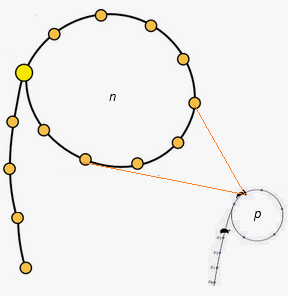
\includegraphics{proyeccion n en p.png}
    \caption{Lo que pasa en $n$ se proyecta en $p$}
    \par\small Fuente: Elaboración propia
\end{figure} \\
Por la naturaleza de $f$ hay un ciclo para $n$ y otro para $p$. Al ser $p$ un factor de $n$, es claro que $n>p$, por lo tanto el ciclo en $p$ será más pequeño, los valores que vayamos probando en $n$, a través de la función con ciclo, serán proyectados internamente en $p$. \\
Será como si la búsqueda se realizara operando directamente en módulo $p$, aún cuando no se conoce $p$ y sólo se trabaja módulo $n$. Al movernos en las secuencias $x_i$ y $y_j$ trabajamos con enteros distintos módulo $n$, sin embargo, por el juego de estructuras, dichos enteros colisionarán antes en $p$, serán congruentes módulo $p$ en algún momento de la secuencia, definitivamente. 

\subsection{Congruencia en $p$ y no congruencia en $n$}
Dado $n$ compuesto e impar, las secuencias $x_i, y_j$ generan ($x,y$) pares de números enteros módulo $n$ que en algún momento entran en un ciclo. \\
Ya se dijo que se espera que dichos números $x,y$ sean congruentes módulo $p$, el factor desconocido de $n$ (tal congruencia se revelaría, nítidamente, aplicándoles en la sombra el módulo $p$). \\
Ahora se añade otra condición, se esperamos además que $x,y$ sean enteros no congruentes módulo $n$. \\
Todo ello cuaja en el siguiente enunciado.

\begin{enunciado} [Extracción de un factor por colisión en Rho de Pollard]\label{enun:extraeFactor}\leavevmode\par 
Sea $n=p \cdot c$, donde $p$ es un factor primo de $n$ y por tanto $p \mid n$. \\ 
Si $x,y$ son tales que \\ 
$x \equiv y \pmod p$ \\ 
$x \not\equiv y \pmod n $ \\ 
Entonces $d = mcd(|x - y|,n)$ satisface $1 < d < n$ y es un factor no trivial de $n$ (múltiplo de $p$ o $p$ mismo)
\end{enunciado}

\begin{proof} Sea $d = mcd(|x - y|,n)$. \\
Si $x \equiv y \pmod p$, entonces por el Enunciado~\ref{enun:congrViaDivisib}, $p \mid (x - y)$. Por lo tanto, $(x-y)=kp$, luego $|x-y|=|kp|=p|k|$, por lo tanto: $p \mid |x-y|$. \\
Como $p \mid n$ entonces $p$ divide a ambos números $|x - y|$ y $n$, es decir, $p \mid |x-y|$ y $p \mid n$. \\
Por el Enunciado~\ref{enun:maspropMcd}.ix: $p \mid mcd(|x - y|,n)$, es decir, $p \mid d$. Luego, por el Enunciado~\ref{enun:propDivisibilidad}.ii: $d \geq p$. \\
Como $p$ es primo, $p > 1$, por lo tanto: $d > 1$. \\
Si $x \nequiv y \pmod n $, entonces $n \nmid (x - y)$. \\
Razonando por contradicción, supongamos que $d = n$. \\
Por lo tanto: $n = mcd(|x - y|,n)$. Y, por supuesto: $n \mid |x - y|$. \\
Luego, $n \mid (x - y)$, lo que contradice $n \nmid (x - y)$. \\
Ello invalida el supuesto y prueba que $d \neq n$. \\
Como $d = mcd(|x - y|,\, n)$, por definición $d \mid n$, luego  por el Enunciado~\ref{enun:propDivisibilidad}.ii: $d \leq n$. \\ 
Como $d \neq n$ y $d \leq n$ entonces: $d < n$. \\
Hemos probado que $1 < d < n$. \\
Como $d \mid n$, por definición, $d$ es un divisor propio no trivial de $n$. \\
Como $p \mid d$, entonces $d=pk'$, es decir, $d= mcd(|x - y|,n)$ es un múltiplo de $p$ (el cual puede ser $p$ mismo, o bien un múltiplo mayor).
\end{proof}

El objetivo no es mostrar que $x \equiv y \pmod p$ , sino aprovechar esa congruencia, cuando ocurre, para obtener un factor no trivial de $n$. No se sabe en qué paso ocurre tal congruencia, eso vive en un mundo al que no se tiene acceso directo, pero se puede razonar sobre él. \\
Lo que sí podemos hacer es calcular, en cada paso, $mcd(|x_i - y_j|, n)$, sin conocer $p$. Si en algún momento ocurre una colisión útil módulo un factor primo $p$ de $n$, antes de que ocurra la congruencia módulo $n$, el enunciado garantiza que el $mcd$ hará visible esa colisión como un factor no trivial de $n$, esa es la causa matemática de que $p$ aflore en el $mcd$. \\
El enunciado es la garantía de que ese cálculo, ciego a p, capturará el evento oculto en el momento en que ocurra, sin él no habría ninguna razón para creer que computar $mcd$'s sucesivos eventualmente revela $p$. \\
Pollard aprovecha una colisión parcial invisible para convertirla, mediante el $mcd$, en un factor visible de $n$, el factor $d$ es $p$ mismo o un múltiplo mayor, no importa, el enunciado garantiza que se obtiene dicho factor. \\
Como $p$ es un factor primo arbitrario de $p$, el razonamiento vale para cualquiera de los factores primos que pueda producir la colisión. \\
Sin esa congruencia parcial, el $mcd$ daría 1 y no serviría.  Sin la no congruencia módulo $n$ tampoco serviría, es el caso cuando el $mcd$ devuelve $n$. Los siguientes enunciados sustentan ello.

\begin{enunciado}
\label{enun:Rhomcd1}\leavevmode\par 
Sea $n=p \cdot c$, donde $p$ es un factor primo de $n$ y por tanto $p \mid n$. \\
Si $mcd(x - y, n) = 1$ entonces $x \nequiv y \pmod{p}$
\end{enunciado}

\begin{proof} Por contradicción. \\
Supongamos que $x \equiv y \pmod{p}$, por el Enunciado~\ref{enun:congrViaDivisib} $p \mid (x - y)$. \\
Es decir, $p \mid n$, también $p \mid (x - y)$. Por el Enunciado~\ref{enun:maspropMcd}.ix: $p \mid mcd(x - y, n)$. \\
Pero $mcd(x - y, n) = 1$. Por lo tanto: $p \mid 1$. \\
Lo que contradice que $p$ sea primo y prueba el enunciado.
\end{proof}

\begin{enunciado}
\label{enun:Rhomcd2}\leavevmode\par 
Sea $n=p \cdot c$, donde $p$ es un factor primo de $n$ y por tanto $p \mid n$. \\
Si $mcd(x - y, n) = n$ entonces $x \equiv y \pmod n$
\end{enunciado}

\begin{proof} Si $mcd(x - y, n) = n$ entonces $n \mid (x-y)$. \\
Luego, por el Enunciado~\ref{enun:congrViaDivisib}: $x \equiv y \pmod n$.
\end{proof}

\subsection{Velocidad de la colisión}
El Enunciado~\ref{enun:extraeFactor} muestra que buscar colisiones módulo $p$ funciona. \\ 
Resta engranar con una estrategia que indique cómo producir tales $x,y$ congruentes de forma eficiente. 
Es vital que sean congruentes módulo $p$, pero lo esencial es cómo generar esos pares de forma sistemática y rápida sin saber nada de $p$ (ahí es donde interviene el epimorfismo, sin él no queda claro por qué iterar módulo $n$ tendría algo que ver con el factor $p$). \\

Sería un error generar dos números $x,y$ completamente al azar en cada paso, calcular $mcd(x-y,n)$ y esperar que salga un valor $d$ tal que $1<d<n$: es un proceso muy lento (peor que buscar divisores uno por uno) y muy improbable (que dos números elegidos al azar difieran exactamente en un múltiplo de un factor de $n$, $x \equiv y \pmod p$, es de una probabilidad $1/p$ muy baja). \\
Pensemos en esta otra hipotética forma de hallar la colisión módulo $p$: guardar todos los valores, al generar uno nuevo compararlo con los anteriores (verificando si son congruentes módulo $p$), esto requiere poner en la lista cada número que va apareciendo para revisar si es congruente con uno que ya salió antes, la computadora se quedaría sin memoria al trabajar con números gigantescos. \\

La ventaja de usar $x_i$ y su subsecuencia $y_j$ (idea desprendida del algoritmo de Floyd para ver si una lista tiene ciclos) es que usa una sola secuencia, la confronta consigo misma y detecta una colisión prácticamente sin usar memoria: si la secuencia entra en un ciclo, $y_j$ (que es $x_{2i}$ que suele denominarse el corredor rápido o liebre) inevitablemente alcanzará a $x_i$ (que suele denominarse el corredor lento o tortuga) dentro del ciclo. No hay necesidad de almacenar toda la secuencia, sólo se requiere recordar dos variables en la memoria en todo momento: la posición actual del lento $x$ y la posición actual del rápido $y$. \\

La función $f$ módulo $n$ sirve para forzar los dos ciclos módulo $n$ y módulo $p$ (que no se ve, pero está ahí). \\
Tarde o temprano encontraremos $x_i \equiv y_j \pmod p $ antes de que $x_i \equiv y_j \pmod n $. \\
El principio del palomar (pigeonhole) dice: si se distibuye más elementos (números, palomas, etc.) que contenedores disponibles, al menos uno de los contenedores contendrá obligatoriamente varios elementos (que colisionan o chocan o se agrupan). \\
Como sólo hay un número finito de valores $p$ (contenedores), por el principio del palomar, al ir generando parejas diferentes (elementos) módulo $n$ ($p+1$ elementos, o más), tarde o temprano obligatoriamente habrá una colisión en el mundo secreto del módulo $p$: necesariamente hay dos índices $i \neq j$ (con $i,j \leq p$) tales que $x_i,y_j$ serán congruentes módulo $p$. \\
Y por la naturaleza del ciclo y su longitud, cada que generemos pares separados por (un múltiplo de) dicha longitud, seguirán existiendo colisiones. \\
Ello es una consecuencia puramente estructural de que el dominio $\Z/p\Z$ es finito y $f$ es una función determinista sobre él. \\

Pero la forma de trabajo de $f$ aporta otro asunto esencial además del ciclo: un análisis probabilista de su comportamiento, la velocidad. \\
¿Cuánto tarda en aparecer esa colisión? \\
$f$ genera una secuencia determinista de apariencia pseudoaleatoria, esto es crucial para aplicar tal análisis probabilístico con ayuda de la paradoja del cumpleaños. \\

\textbf{La paradoja del cumpleaños} \\
Sea un año de 365 días. \\
Dado un grupo de $N$ personas, hallaremos la probabilidad de que al menos dos personas cumplan años el mismo día. \\
Lo haremos hallando la probabilidad de que todos tengan cumpleaños distintos. \\
Cada persona tiene un cumpleaños igualmente probable e independiente. \\
La primera persona puede cumplir años en cualquiera de los 365 días: probabilidad 1. \\
La segunda persona debe caer en un día distinto:  probabilidad $\frac{364}{365}$. \\
Etc. \\
Probabilidad de que todos los $N$ cumpleaños sean distintos (P): \\
P = $\frac{365}{365} \cdot \frac{364}{365} \cdot \frac{363}{365} \cdots \frac{365-N+1}{365} = \prod_{i=0}^{N-1}\frac{365-i}{365} = \prod_{i=0}^{N-1}(1-\frac{i}{365})$ \\
Con $N=23, P=0.461655742$. \\
La probabilidad de que al menos dos coincidan es el complemento: $1-P$. \\
Con $N=23, 1-P=0.538344257$. \\
Con solo 23 personas, la probabilidad de que dos compartan cumpleaños, leída como porcentaje, es mayor al 50\%. \\

Aplicamos la misma idea para el caso de la colisión módulo $p$, la probabilidad $P$ de que, dados $k$ números, todos sean distintos es: \\
$P = \prod_{i=0}^{k-1}(1-\frac{i}{p})$ \\
$\ln P = \ln \prod_{i=0}^{k-1}(1-\frac{i}{p}) \qquad \;$ // aplicando logaritmo \\
$= \sum_{i=0}^{k-1}\ln\left(1-\frac{i}{p}\right) \qquad\qquad$  // propiedad de logaritmo \\
$\approx -\sum_{i=0}^{k-1}\frac{i}{p} \qquad\qquad\qquad \,\;$  // con $p$ grande $(i/p)\rightarrow 0$ y $\ln(1-x) \approx -x$ \\
$=- \frac{1}{p} \sum_{i=0}^{k-1}i$ \\
$ = -\frac{k(k-1)}{2p}$ \\
$\approx -\frac{k^2}{2p}$ \\
Es decir, $\ln P \approx -\frac{k^2}{2p}$. Luego, $P \approx e^{-k^2/(2p)}$. \\
La probabilidad de que al menos dos enteros colisionen es el complemento: \\
$1 - P \approx 1 - e^{-k^2/(2p)}$. \\
El valor de $k$ donde $1-P$ empieza a ser, visto como porcentaje, mayor al $50\%$ o, lo que es lo mismo, el valor de $k$ donde $P$ empieza a ser mayor a $0.5$, es decir, donde colisionar pasa a ser más probable que no, es: \\
$e^{-k^2/(2p)} > \frac{1}{2} \qquad \quad \, \,$ // aplicando logaritmo \\
$\ln e^{-k^2/(2p)} > \ln \frac{1}{2} \qquad$ \\
${-k^2/(2p)} > \ln \frac{1}{2} \qquad$ // obvio \\
$-k^2 > (2p) \ln \frac{1}{2} \qquad \,$ // $\cdot(-1)$  \\
$k^2 < (2p) \ln \frac{1}{2} \qquad \, \, \, \;$ // aplicando raíz cuadrada \\
$k < \sqrt 2 \sqrt p \sqrt{\ln \frac{1}{2}}\qquad$ // $c=\sqrt 2 \sqrt{\ln \frac{1}{2}}$ \\
$k < c \sqrt p$ \\
Es decir, el número $k$ de iteraciones antes de una (probable) colisión (que revele un factor de $n$) es del orden $O(\sqrt{p})$ y proviene de la misma lógica de la paradoja del cumpleaños. \\
Si cambiamos la meta de que $P>0.5$ por, digamos, $P>0.9$ y repetimos el cálculo, la constante cambiará pero el orden seguirá siendo $O(\sqrt{p})$. \\
Hemos simplificado la presentación, en vez de un umbral lo que corresponde es calcular el valor esperado del número de iteraciones hasta la colisión, que se obtiene así ($X$ es una variable aleatoria que representa el número de iteraciones en el que efectivamente ocurre la colisión): \\
$E[X] \approx \int_0^\infty P(X>k)\,dk \approx \int_0^\infty e^{-k^2/(2p)}\,dk = \sqrt{\frac{\pi}{2}} \sqrt{p}$. \\
Sin embargo, la presentación que se hizo es más sencilla y cumple el propósito. \\

El Enunciado~\ref{enun:cotaRaizdeN} muestra que el entero compuesto $n$ tiene un divisor $p$ tal que $p \leq \sqrt{n}$. \\
Por lo tanto: $\sqrt{p} \leq \sqrt (\sqrt{n})=n^{\frac{1}{4}}$. \\
Por ello la complejidad temporal promedio para encontrar un factor primo de $n$ se dice que es del orden O($n^{1/4}$) con este algoritmo.

\section{Fundamentos de las cribas}
En el contexto de la teoría de números, las cribas constituyen una familia de algoritmos deterministas diseñados para identificar números primos dentro de un conjunto finito de enteros mediante un proceso de filtrado sistemático. A diferencia de las pruebas de primalidad individuales, que verifican propiedades específicas de un solo número, una criba opera por eliminación: partiendo de una lista de candidatos, descarta iterativamente aquellos que son múltiplos de primos menores, dejando únicamente los números primos como resultado. Esta metodología, cuyo exponente clásico es la Criba de Eratóstenes, se fundamenta en principios aritméticos de divisibilidad y constituye la herramienta estándar para la generación eficiente de listas de primos.\\
La clasificación y evolución de estos métodos abarcan desde las aproximaciones más antiguas hasta algoritmos modernos optimizados, como la Criba de Atkin o las cribas segmentadas, cada uno con distintas complejidades computacionales y requerimientos de memoria. Comprender los fundamentos de estas técnicas no solo implica asimilar el criterio lógico de selección y marcado de múltiplos, sino también distinguir entre los distintos enfoques algorítmicos.\\
Es más útil, en varios casos, acompañar la teoría al momento de describir cribas específicas, así lo haremos, salvo algunos resultados que siguen a continuación.

\begin{enunciado}[Techo (ceil) como parte entera (floor)]\label{enun:ceilequivalentefloor}\leavevmode\par
Sea $b \geq 1$. $\lfloor \frac{a-1+b}{b} \rfloor  = \lceil \frac{a}{b}\rceil$
\end{enunciado}

\begin{proof}
Por el algoritmo de la división, Enunciado~\ref{enun:algDivision}:\\
$a = qb+r$, donde $q$ es el cociente y $r$ es el residuo, con $0 \leq r<b$.\\
Caso $r=0$:\\
$\lceil \frac{a}{b} \rceil$\\
$= \lceil \frac{qb}{b} \rceil$   \; \; \; \;  \; \; \; \; \; \; \; \;  // pues $a = qb+r$ y $r=0$\\
$= \lceil q \rceil = q$ \; \; \; \;  \; \; \; \; \; \;  // obvio\\
$= (q+1)-1$ \; \; \;  \; \; \; \;  // obvio \\
$= (q+1)+ \lfloor \frac{-1}{b} \rfloor$ \; \; \; \; //  pues $b \geq 1$ y $\lfloor \frac{-1}{b} \rfloor= -1$ \\
$= q+1+ \lfloor \frac{r-1}{b} \rfloor$ \; \; \; \;  \; //  pues $r=0$ \\
$=  \lfloor q+1+ \frac{r-1}{b} \rfloor$ \; \; \; \; \; // pues $q+1$ es entero \\
$=  \lfloor \frac{qb+b+ r -1}{b} \rfloor$  \; \; \; \;  \; \; \; \;  // obvio \\
$=  \lfloor \frac{qb+r+b-1}{b} \rfloor$ \; \; \; \;  \; \; \; \;  // obvio \\
$=  \lfloor \frac{a+b -1}{ b} \rfloor$ \; \; \; \;  \; \; \; \; \; \;  // pues  $a = qb+r$ \\
$=  \lfloor \frac{a-1+b}{b} \rfloor$ \; \; \; \; \; \;  \; \; \; \;   // obvio \\
Caso $r>0$:\\
Como $0<r<b$, entonces $1 \leq r$ y, como $r-1<r$ y $r<b$ entonces $r-1<b$.\\
$\lceil \frac{a}{b} \rceil$\\
$= \lceil \frac{qb+r}{b} \rceil$ \; \; \;  \; \; \; \; \; \; \; \;  // pues $a = qb+r$\\
$= \lceil q+ \frac{r}{b} \rceil$   \; \; \; \; \; \; \; \; \; \; // obvio \\
$= q+ \lceil \frac{r}{b} \rceil$ \; \; \; \; \; \; \; // pues $q$ es entero \\
$= q+1$  \; \; \; \; \; \; \; \; \; // pues $r<b$ y $\lceil \frac{r}{b} \rceil = 1$ \\
$= q+1+0$ \; \; \; \; \; \; // obvio \\
$= q+1+ \lfloor \frac{r-1}{b} \rfloor$ \; \; \; // pues  $r-1<b$ y $\lfloor \frac{r-1}{b} \rfloor = 0$
$=  \lfloor q+1+ \frac{r-1}{b} \rfloor$ \; \; \; // pues $q+1$ es entero \\
$=  \lfloor \frac{qb+b+ r -1}{b} \rfloor$  \; \; \; \;  \;  // obvio \\
$=  \lfloor \frac{qb+r+b-1}{b} \rfloor$ \; \; \; \; \;  // obvio \\
$=  \lfloor \frac{a+b -1}{ b} \rfloor$ \; \; \; \;  \; \; \;  // pues  $a = qb+r$ \\
$=  \lfloor \frac{a-1+b}{b} \rfloor$ \; \; \; \; \; \; \;   // obvio
\end{proof}

\begin{enunciado}[$p ^{2}$ impar]\label{enun:p2impar}\leavevmode\par
Si $p$ es impar entonces $p^2$ es impar
\end{enunciado}

\begin{proof}
Como $p$ es impar, entonces $p = 2k+1$. \\
$p ^{2} = (2k+1)^{2} = 4k^{2}+4k+1 = 2(k^{2}+2k)+1$, que evidentemente es impar. 
\end{proof}

\begin{enunciado}[Suma de números pares/impares]\label{enun:parimpar}\leavevmode\par
La sumas de dos números pares o dos números impares es par. La suma de un número impar con uno par es impar.
\end{enunciado}

\begin{proof}
Para $a$ y $b$ pares: $a = 2k$, $b = 2q$. Luego, $a+b = 2k+2q = 2(k+q)$ que evidentemente es par. \\
Para $a$ y $b$ impares: $a = 2k+1$, $b = 2q+1$. Luego, $a+b = 2k+1+2q+1 = 2k+2q+2 = 2(k+q+1)$ que evidentemente es par. \\
Para $a$ par y $b$ impar: $a = 2k$, $b = 2q+1$. Luego, $a+b = 2k+2q+1 = 2(k+q)+1$ que evidentemente es impar.
\end{proof}

\subsection{Elementos para la criba cuadrática}
\label{subsec:Fundcuadratica}
En este caso la criba no pretende hallar números primos sino enteros con $B$-suavidad. 

\begin{definicion} [$B$-suavidad]\label{def:Bsuavidad}
La definición genérica dice que un entero es $B$-suave si todos sus factores primos son menores o iguales que el entero $B$. \\
Pero en la criba cuadrática un entero es $B$-suave si todos sus factores primos están en un conjunto base de primos llamado la base $B$. \\
Decir que un entero sea $B$-suave es equivalente a decir que el entero tenga $B$-suavidad.
\end{definicion}

\begin{enunciado}[Principio general]\label{enun:PpioGeneral}\leavevmode\par
Sea $n$ impar y compuesto. \\
Si existen enteros $x,y$ tales que $x^2 \equiv y^2 \pmod n \,$, $\, x \nequiv \pm  y \pmod n$ \\
entonces $d=mcd(x-y,n)$ es un factor no trivial de $n$, es decir, $1< d <n$
\end{enunciado}

\begin{proof} \, \\
Como $x^2\equiv y^2\pmod n$, por el Enunciado~\ref{enun:congrViaDivisib} $n \mid (x^2-y^2)$, es decir, $n \mid (x-y)(x+y)$. \\
Sea $d=mcd(x-y,n)$. \\
Queremos demostrar que $1<d<n$. \\
$d>1$: \\
Supongamos, por contradicción, que $d=1$. \\
Como $x^2 \equiv y^2\pmod n$, además $-y^2  \equiv -y^2\pmod n$, entonces por el Enunciado~\ref{enun:propCongru}.iii: \\
$x^2-y^2 \equiv y^2-y^2 \pmod n$, es decir: $x^2-y^2 \equiv 0 \pmod n$. \\
Como $x^2-y^2 = (x-y)(x+y)$, entonces: \\
$(x-y)(x+y) \equiv 0 \pmod n$. \\
Como $d=1$, entonces $mcd(x-y,n)=1$. \\
Por el Enunciado~\ref{enun:existInvModular} $x-y$ tiene inverso módulo $n$. \\
Es decir, existe $a$ tal que $a(x-y) \equiv 1 \pmod n$. \\
Como $(x-y)(x+y) \equiv 0 \pmod n$, además $a \equiv a \pmod n$, entonces por el Enunciado~\ref{enun:propCongru}.iv: \\
$a(x-y)(x+y) \equiv a \cdot 0 \pmod n$. \\
Es obvio que $a \cdot 0 = 0$. Como $a(x-y) \equiv 1 \pmod n$ entonces por el Enunciado~\ref{enun:propCongru}.viii: \\
$(x+y) \equiv 0 \pmod n$. \\
Es decir, $x\equiv-y\pmod n$, contradiciendo la hipótesis $x \nequiv \pm y \pmod n$. \\
Por tanto, $d>1$. \\
$d<n$: \\
Supongamos, por contradicción, que $d=n$. \\
Es decir, $mcd(x-y,n)=n$. \\
Entonces $n \mid (x-y)$, por el Enunciado~\ref{enun:congrViaDivisib} $x \equiv y \pmod n$, lo cual contradice $x \nequiv \pm y \pmod n$. \\
Así que $d<n$. \\
Por consiguiente, $1< mcd(x-y,n) < n$. \\
Es decir, $d$ es un factor no trivial de $n$.
\end{proof}

El principio general incluye como supuesto que $x \nequiv \pm  y \pmod n$ pues de lo contrario no se obtiene un factor no trivial.

\begin{enunciado}[Por qué la congruencia es estéril]\label{enun:congrEsteril}\leavevmode\par
a) Si $x \equiv y \pmod n$, entonces $\gcd(x-y, n) = n$. \\
b) Si $x \equiv -y \pmod n$, entonces $\gcd(x+y, n) = n$.
\end{enunciado}

\begin{proof} \, \\
a) Como $x \equiv y \pmod n$, por el Enunciado~\ref{enun:congrViaDivisib}, $n \mid (x-y)$. \\
Como $n \mid n$, entonces $mcd(x-y, n) = n$. \\
b) Como $x \equiv -y \pmod n$, por el Enunciado~\ref{enun:congrViaDivisib}, $n \mid (x-(-y))$, es decir, $n \mid (x+y)$. \\
Como $n \mid n$, entonces $mcd(x+y,n) = n$. \\
En ambos casos el factor $n$ es trivial.
\end{proof}

\begin{enunciado}[Por qué la congruencia es estéril, segunda parte]\label{enun:congrEsteril2}\leavevmode\par
a) Sea $n$ un entero impar y compuesto. 
\\ Sea $B=\{p_{1},p_{2},\dots ,p_{m}\}$ una base primos tales que $\forall p_{i} \in B \,\, p_{i} \nmid n$. \\
Sean $x,y$ enteros tales que $x^{2} \equiv y^{2}\pmod n$. \\
Supongamos que $y$ se construye como producto de potencias de primos de $\mathcal{B}$ (es decir, $y$ es $B$-suave). \\
Supongamos además que: \\
a) $x \equiv y \pmod n$ entonces $mcd(x+y,n)=1$. \\
b) $x \equiv -y \pmod n$ entonces $mcd(x-y,n)=1$.
\end{enunciado}

\begin{proof} \, \\
Como $n$ es impar, $mcd(2,n)=1$, por tanto por el Enunciado~\ref{enun:maspropMcd}.x $mcd(2y,n)=mcd(y,n)$. \\
Por hipótesis, todo primo que divide a $y$ pertenece a $B$, y ningún primo de $B$ divide a $n$. Por lo tanto, $mcd(y,n)=1$. \\
a) Como $x \equiv y\pmod n$ y como $y \equiv y \pmod n$, por el Enunciado~\ref{enun:propCongru}.iii: $x+y\equiv 2y\pmod n$. \\
Luego, por el Enunciado~\ref{enun:maspropMcd}.xi, $mcd(x+y,\, n)=mcd(2y,n)$. \\
En consecuencia $mcd(x+y,n)=1$. \\
b) Como $x \equiv -y \pmod n$, $-y \equiv -y \pmod n$, por el Enunciado~\ref{enun:propCongru}.iii: $x-y \equiv -2y\pmod n$. \\
Luego, por el Enunciado~\ref{enun:maspropMcd}.xi y por el Enunciado~\ref{enun:propMcd}.ii: \\
$mcd(x-y,n)=mcd(-2y,n)=mcd(2y,n)$. \\
En consecuencia $mcd(x-y,n)=1$. \\
En ambos casos, si $mcd(x-y,n)=n$ (o $mcd(x+y,n)=n$), calcular $mcd(x+y,n)$ (o $mcd(x-y,n)$) es redundante, pues necesariamente dará el factor trivial $1$.
\end{proof}

\begin{enunciado}[Por qué la congruencia es estéril, tercera parte]\label{enun:congrEsteril3}\leavevmode\par
Sea $n$ un entero impar y compuesto. \\
Sean $x, y$ tales que $x^2 \equiv y^2 \pmod n$. \\
Entonces: \\
1) $mcd(x-y, n) = 1 \quad\Longleftrightarrow\quad x \equiv -y \pmod n \;\text{ y }\; mcd(y,n)=1$ \\
2) $mcd(x+y, n) = 1 \quad\Longleftrightarrow\quad x \equiv y \pmod n \;\text{ y }\; mcd(y,n)=1$
\end{enunciado}

\begin{proof}
Como $x^2 \equiv y^2 \pmod n$, por el Enunciado~\ref{enun:congrViaDivisib}: $n \mid (x-y)(x+y) \qquad$ (*) \\
\textit{1}) \\
$\Rightarrow$) Supongamos $mcd(x-y,n) = 1$. \\
De (*) y por el Enunciado~\ref{enun:propMcd}.viii, lema de Euclides: $n \mid (x+y)$, es decir, $n \mid (x-(-y))$. \\
Luego, por el Enunciado~\ref{enun:congrViaDivisib}, $x \equiv -y \pmod n$. Además $-y \equiv -y \pmod n$. \\
Entonces, por el Enunciado~\ref{enun:propCongru}.iii: $x - y \equiv -2y \pmod n$. \\
Luego, por el Enunciado~\ref{enun:maspropMcd}.xi, $mcd(x-y,n)=mcd(-2y,n)$. \\
Y por el por el Enunciado~\ref{enun:propMcd}.ii: $mcd(x-y,n)=mcd(2y,n)$. \\
Como $n$ es impar, $mcd(2,n)=1$, por tanto por el Enunciado~\ref{enun:maspropMcd}.x $mcd(2y,n)=mcd(y,n)$. \\ 
Es decir: $mcd(x-y,n)=mcd(y,n)$. Como $mcd(x-y,n) = 1$, entonces: \\
$mcd(y,n) = 1$. \\
$\Leftarrow$) Supongamos ahora que $x \equiv -y \pmod n$ y $mcd(y, n) = 1$. \\
Como $-y \equiv -y \pmod n$, de ello y de $x \equiv -y$ se sigue, por el Enunciado~\ref{enun:propCongru}.iii, que: \\
$x - y \equiv -2y \pmod n$. \\
Luego, por el Enunciado~\ref{enun:maspropMcd}.xi, $mcd(x-y,n)=mcd(-2y,n)$. \\
Y por el por el Enunciado~\ref{enun:propMcd}.ii: $mcd(x-y,n)=mcd(2y,n)$. \\
Como $n$ es impar, $mcd(2,n)=1$, por tanto por el Enunciado~\ref{enun:maspropMcd}.x $mcd(2y,n)=mcd(y,n)$. \\ 
Es decir: $mcd(x-y,n)=mcd(y,n)$. Como $mcd(y,n) = 1$, entonces: \\
$mcd(x-y,n) = 1$. \\
\textit{2}) \\
El razonamiento es completamente análogo.
\end{proof}

\subsubsection{Raíces cuadráticas, criterio de Euler y símbolos de Legendre y Jacobi} 
\label{subsubsec:JacobiYmas}
La Definición~\ref{def:congrcuadraticaraizde1modn} introduce la congruencia cuadrática pura: $x^2 \equiv a \pmod m$. \\
Se tiene la siguiente definición asociada.

\begin{definicion}[Definición amplia de residuo cuadrático] \, \\
$a$ es un residuo cuadrático módulo $m$ si existe un entero $x$ tal que $x^2 \equiv a \pmod {m}$.
\end{definicion}

\begin{ejemplo}
$9$ es un residuo cuadrático módulo $21$, según la definición amplia, pues existe $x=3$ tal que $3^2 \equiv 9 \pmod {21}$.
\end{ejemplo}

Se tiene esta otra definición asociada que podemos denominar definición estricta pues exige que $mcd(a,m)=1$.

\begin{definicion}[Residuo cuadrático]\label{def:residuocuadr} \, \\
$a$ coprimo con $m$ es un residuo cuadrático módulo $m$ si la congruencia $x^2  \equiv a \pmod {m}$ tiene solución.
\end{definicion}

\begin{ejemplo}
$9$ no es un residuo cuadrático módulo $21$ estricto pues $mcd(9,21)=3$. \\
$5$ es un residuo cuadrático módulo $11$ pues existe $x=4$ tal que $4^2 \equiv 5 \pmod {11}$ y $mcd(5,11)=1$.
\end{ejemplo}

$a$ es un cuadrado módulo $m$ es, quizás, un mejor nombre, pero en la  historia siempre se ha dicho que $a$ es un residuo cuadrático módulo $m$, de modo que respetaremos ello. \\
 
La definición estricta es la definición usual pues con la exigencia de coprimalidad, como se muestra en el Anexo~\ref{anexo:iso}, $(\Z/m\Z)^{*}$ es un grupo multiplicativo. \\
Las características de un grupo multiplicativo son altamente deseables, por ejemplo, todos sus elementos tienen inverso. El conjunto de residuos cuadráticos módulo $m$ es un subgrupo de dicho grupo multiplicativo, como lo muestra el siguiente enunciado.

\begin{enunciado} El conjunto de los residuos cuadráticos módulo $m$ que son coprimos con $m$ forma un subgrupo del grupo multiplicativo $(\Z/m\Z)^{*}$
\end{enunciado}

\begin{proof} Un elemento $a \in (\Z/m\Z)^*$  es un residuo cuadrático si existe un $ x \in (\Z/m\Z )^*$  tal que: \\
$ x^{2}\equiv a \pmod m$ \\
Este conjunto  es un subgrupo de $ (\Z/m\Z )^*$ pues verifica sus propiedades fundamentales: \\
. Identidad: El $1$  siempre es un residuo cuadrático porque $1^2 \equiv 1 \pmod m$. \\
. Cierre bajo el producto: Si $a$  y $ b$  son residuos cuadráticos, existen $ x$  e $ y$  tales que $x^2 \equiv a$  y $y^2 \equiv b$ . Entonces: $a \cdot b\equiv x^{2}\cdot y^{2}\equiv (x\cdot y)^{2} \pmod m$ .\\
Como $ (x \cdot y)^2$  es un cuadrado perfecto, $ a \cdot b$  también es un residuo cuadrático. \\
. Inversos: Si $a$  es un residuo cuadrático ($x^2 \equiv a$ ), podemos multiplicar ambos lados por el inverso de $x^{2}$  (que es $(x^{-1})^2$): $a\cdot (x^{-1})^{2}\equiv x^{2}\cdot (x^{-1})^{2}\equiv 1 \pmod m$. \\ 
Por lo tanto, $a^{-1} \equiv (x^{-1})^2 \pmod m$ , por lo que el inverso de $a$  también es un residuo cuadrático y pertenece al subgrupo.
\end{proof}

El caso particular  $x^2  \equiv n \pmod {p}$ con $p$ primo y $n$ un entero impar y compuesto es relevante pues se utiliza en la factorización de $n$ con la criba cuadrática. \\

En vez de decir que existe un entero $x$ tal que $x^2  \equiv n \pmod {p}$ (suficiente para decir que $n$ es un residuo cuadrático módulo $p$), también es usual decir hallar las raíces de $x^2  \equiv n \pmod {p}$. \\
Con $p$ primo cada elemento distinto del 0 del conjunto de base tiene inverso multiplicativo, con ello -como se ve en el Anexo~\ref{anexo:iso}- $(\Z/m\Z)^{*}$ es un cuerpo. \\
Es decir, no existen divisores de cero: si $ab \equiv 0 \pmod{p}$, entonces necesariamente $a \equiv 0$ o $b \equiv 0$. \\

Resolver $x^2 \equiv 1 \pmod{p}$ es resolver $x^2 - 1 \equiv 0 \pmod{p}$, es decir, $(x-1)(x+1) \equiv 0 \pmod{p}$. \\
Sin divisores de cero, el producto solo puede ser cero si uno de los factores lo es: \\
$x-1 \equiv 0 \pmod{p}$, es decir, $x \equiv 1 \pmod{p}$ \\
$x+1 \equiv 0 \pmod{p}$, es decir, $x \equiv -1 \pmod{p}$ \\
Al ser $x^2 - 1$ un polinomio de grado 2 no puede tener más de 2 raíces distintas.

\begin{ejemplo}
$2310 \bmod 13 = 9$. \\
Luego, $2310$ es un residuo cuadrático módulo $13$ pues existe $x=3$ tal que $3^2  \equiv 2310 \pmod {13}$. \\
Como $10^2 \bmod 13 = 100 \bmod 13 = 9$, con igual validez puede decirse que $2310$ es un residuo cuadrático módulo $13$ pues existe $x=10$ tal que $10^2  \equiv 2310 \pmod {13}$. \\
Dicho de la otra forma: hallemos las raíces de $x^2  \equiv 2310 \pmod {13}$. La raíces son $x=3,10$, hay solución.
\end{ejemplo}

\begin{ejemplo} Sea $p=11$. \\
Trabajaremos con el conjunto $\{1, 2, \dots, p-1\} = \{1, 2, \dots, 10\}$. \\
Al elevar al cuadrado los números del 1 al 10 y calcular su resto módulo 11, obtenemos:
\begin{itemize}
    \item $1^2 \equiv 10^2 \equiv 1 \pmod{11}$
    \item $2^2 \equiv 9^2 \equiv 4 \pmod{11}$
    \item $3^2 \equiv 8^2 \equiv 9 \pmod{11}$
    \item $4^2 \equiv 7^2 \equiv 5 \pmod{11}$
    \item $5^2 \equiv 6^2 \equiv 3 \pmod{11}$
\end{itemize}
El conjunto de residuos cuadráticos módulo 11 es $\{1, 3, 4, 5, 9\}$. 
Exactamente la mitad (5 de 10) de los elementos de $\{1, 2, \dots, 10\}$ son residuos cuadráticos distintos. \\
Nótese que $x^2 \equiv (p-x)^2 \pmod{p}$, es decir, $x^2 \equiv (11-x)^2 \pmod{11}$. \\
Es decir, cada número $x$ y su complemento $11-x$ producen el mismo residuo cuadrático módulo 11.
\end{ejemplo}

\begin{enunciado} [Número de residuos cuadráticos con $p$ primo]\label{enun:numResiduos}\leavevmode\par
Para $p$ un primo impar, exactamente la mitad $\frac{p-1}{2}$ de los números en el conjunto $\{1, 2, \dots, p-1\}$ son residuos cuadráticos distintos.
\end{enunciado}

\begin{proof}
Los cuadrados módulo $p$ de los números en $\{1,2,\dots,p-1\}$ son: \\
$1^2, \dots, (p-1)^2 \pmod{p}.$ \\
Como $(p-x)^2 = p^2 -2xp + x^2$, además que $p^2 -2xp + x^2 \equiv x^2 \pmod p$: \\
$x^2 \equiv (p-x)^2 \pmod{p}$ \\
Es decir, cada número $x$ y su complemento $p-x$ producen el mismo residuo cuadrático módulo $p$. \\
Por ello, los números $1,2,\dots,p-1$ se pueden agrupar en $\frac{p-1}{2}$ pares: \\
$(1, p-1), (2, p-2), \dots, \left(\tfrac{p-1}{2}, \tfrac{p+1}{2}\right)$. \\
Cada par genera el mismo residuo cuadrático módulo $p$.  \\
Por lo tanto, de los $p-1$ residuos cuadráticos, sólo hay $\frac{p-1}{2}$ valores distintos. \\
Tampoco es posible que dos pares distintos den el mismo resultado. En efecto, sean $x,y$ elementos de distintos pares. Supongamos que $x^2 \equiv y^2 \pmod p$, es decir, $x^2 - y^2 \equiv 0 \pmod p$. \\
Por la distributividad del producto sobre la suma: $x^2 - y^2 = (x-y)(x+y) $. \\
Entonces: $(x-y)(x+y) \equiv 0 \pmod{p}$. \\
Como $\Z/p\Z$, es un cuerpo, en la la Sección~\ref{sec:polinomios} se muestra que no tiene divisores de cero. \\
Por lo tanto, si $(x-y)(x+y) \equiv 0 \pmod{p}$, entonces: \\
$(x-y) \equiv 0 \pmod{p}$, o $(x+y) \equiv 0 \pmod{p}$. \\
Es decir: \\
$x \equiv y \pmod{p}$, o \\
$x \equiv -y \pmod{p}$, de donde se tiene: $x \equiv p-y \pmod{p}$.\\
Lo que contradice que $x,y$ sean de distintos pares. \\
Luego, todos los $\frac{p-1}{2}$ resultados tienen que ser estrictamente diferentes entre sí. \\
\end{proof}

El \textbf{Criterio de Euler} es un resultado de la teoría de números que permite determinar si un número es un residuo cuadrático módulo un primo $p$ sin necesidad de encontrar explícitamente sus raíces.

\begin{enunciado}[Criterio de Euler]\label{enun:criterioEuler}\leavevmode\par
Sea $p$ un número primo impar y sea $n$ un entero tal que $mcd(n,p) = 1$ (es decir, $p \nmid n$). Entonces: \\
$n^{\frac{p-1}{2}} \equiv
\begin{cases}
\,\,\; 1 \pmod{p} & \text{si } n \text{ es un residuo cuadrático módulo } p \\
-1 \pmod{p} & \text{si } n \text{ no es un residuo cuadrático módulo } p
\end{cases}$
\end{enunciado}

\begin{proof}
Por el Enunciado~\ref{enun:teorFermat} (pequeño teorema de Fermat) $n^{p-1} \equiv 1 \pmod p$. \\
Como $n^{p-1} = \left(n^{\frac{p-1}{2}}\right)^2$ entonces $\left(n^{\frac{p-1}{2}}\right)^2 \equiv 1 \pmod{p}$. \\
Como $-1 \equiv -1 \pmod{p}$, por el por el Enunciado~\ref{enun:propCongru}.iii: $\left(n^{\frac{p-1}{2}}\right)^2 - 1 \equiv 0 \pmod{p}$. \\
Sea $b = n^{\frac{p-1}{2}}$, entonces: $b^2 - 1 \equiv 0 \pmod{p}$. \\
Como se muestra en la Sección~\ref{sec:polinomios} $p(x)=x^2 - 1$ se puede factorizar como $p(x) = (x-1)(x+1)$. \\
Entonces: $(b-1)(b+1) \equiv 0 \pmod{p}$. \\
Como $\Z/p\Z$, es un cuerpo, en la misma sección se muestra que no tiene divisores de cero. Por lo tanto: \\
Si $(b-1)(b+1) \equiv 0 \pmod{p}$, entonces: $b-1 \equiv 0 \pmod{p}$, o $b+1 \equiv 0 \pmod{p}$. \\
Es decir: \\
$b \equiv 1 \pmod{p}$, o \\
$b \equiv -1 \pmod{p}$. \\
Es decir: \\
$n^{\frac{p-1}{2}} \equiv 1 \pmod{p}$, o \\
$n^{\frac{p-1}{2}} \equiv -1 \pmod{p}$. \\
Supongamos que $n$ es un residuo cuadrático. \\
Es decir, existe $x$ tal que $x^2 \equiv n \pmod{p}$. \\
Entonces, por el Enunciado~\ref{enun:propCongru}.ix: $(x^2)^{\frac{p-1}{2}} \equiv n^{\frac{p-1}{2}}$. Es decir: \\
$n^{\frac{p-1}{2}} \equiv x^{p-1}$. \\
Por el Enunciado~\ref{enun:teorFermat} (pequeño teorema de Fermat): $x^{p-1} \equiv 1 \pmod{p}$. La aplicación del pequeño teorema de Fermat es correcta pues $p \nmid x$.
En efecto, suponer que $p \mid x$, implica que $p \mid x^2$, lo que implica que $p \mid n$, contradiciendo que $mcd(n,p)=1$. \\
Así, si $n$ es un residuo cuadrático módulo $p$, el resultado es $1$: $n^{\frac{p-1}{2}} \equiv 1 \pmod{p}$. \\
Supongamos que $n$ no es un residuo cuadrático. \\
Sea $g(x) = x^{\frac{p-1}{2}} - 1$. \\
Tomemos un $b \in \{1,2,\dots,p-1\}$ que sea residuo cuadrático. \\
Con un razonamiento idéntico al caso anterior: $b^{\frac{p-1}{2}} \equiv 1 \pmod{p}$. \\
Es decir, todo residuo cuadrático es raíz de $g(x)$. \\
Por el Enunciado~\ref{enun:numResiduos}, para $p$ primo impar hay exactamente $\frac{p-1}{2}$ residuos cuadráticos. \\
Por el Enunciado~\ref{enun:numRaices}, $g(x)$  tiene a lo sumo $\frac{p-1}{2}$ raíces distintas, \\
Por lo tanto las raíces de $g(x)$ son exactamente los residuos cuadráticos y ningún otro elemento de $\{1,2,\dots,p-1\}$ es raíz. \\
Como $n$ no es residuo cuadrático, entonces no es raíz de $g(x)$, es decir, $n^{\frac{p-1}{2}} \not\equiv 1 \pmod p$. \\
Como $n^{\frac{p-1}{2}} \equiv 1 \pmod{p}$ o $n^{\frac{p-1}{2}} \equiv -1 \pmod{p}$, la única alternativa restante es $n^{\frac{p-1}{2}} \equiv -1 \pmod p$. \\
Así, si $n$ no es un residuo cuadrático módulo $p$, el resultado es $-1$: $n^{\frac{p-1}{2}} \equiv -1 \pmod{p}$. 
\end{proof}

El criterio de Euler da un algoritmo eficiente, mediante exponenciación rápida, para decidir si $n$ es residuo cuadrático módulo $p$, sin necesidad de probar todos los cuadrados. \\
Aunque hay otro modo igual o más eficiente para determinar ello. Requiere algo de notación adicional y resultados teóricos esenciales. \\

Cuando $p \mid n$: $p \mid (n-0)$. Por el Enunciado~\ref{enun:congrViaDivisib}: $n \equiv 0 \pmod p$. De modo que por el Enunciado~\ref{enun:congrEquiv} (transitividad de la relación de congruencia): $x^2  \equiv n \pmod {p}$ se reduce a $x^2  \equiv 0 \pmod {p}$, cuya unica solución es la trivial $x  \equiv 0 \pmod {p}$. \\
Es un caso degenerado. \\
Cuando $p \mid n$, entonces $mcd(p,n)>1$, por lo tanto $n$ no tiene inverso (no es unidad) módulo $p$, por lo que \underline{está fuera del dominio} en el que tiene sentido clasificar a $n$ como que sea o no sea residuo cuadrático; ni siquiera decir “caso degenerado” es propio: simplemente no aplica la noción de residuo cuadrático porque la definición está reservada al grupo multiplicativo $(\Z/n\Z)^{*}$.

El \textbf{símbolo de Legendre} $\legs{a}{p}$ es una función que permite identificar el carácter cuadrático de un número, para $p$ un primo impar se define como: \\
$\legs{n}{p} =
\begin{cases}
\,\,\; 1 & \text{si } n \text{ es un residuo cuadrático} \bmod p \\
-1 & \text{si } n \text{ no es un residuo cuadrático} \bmod p \\
\,\,\; 0 & \text{si } p \mid n \text{ (} $n$ \text{ fuera del dominio)}
\end{cases}$ 

\begin{ejemplo} \, \\
Sea $p=11$. \\
$\legs{3}{11} = 1$, pues $3$ es un  residuo cuadrático módulo $11$ (existe $x=5$ tal que $5^2 \equiv 3 \pmod{11}$). \\
$\legs{6}{11} = -1$, pues $6$ no es un  residuo cuadrático módulo $11$ (no existe $x$ tal que $x^2 \equiv 6 \pmod{11}$). \\
$\legs{22}{11} = 0$, pues $11 \mid 22$, $22$ está fuera del dominio. \\
\end{ejemplo}

Se puede calcular el símbolo de Legendre con un cálculo previo del $mcd(n,p)$ y en caso de ser $1$, vía el criterior de Euler. \\
De hecho es aceptable y usual una definición alterna con tal criterio: \\
$\legs{n}{p} \equiv n^{\frac{p-1}{2}} \pmod p$ \\
Con el plus de que si $\legs{n}{p}=0$, entonces $n^{\frac{p-1}{2}} \equiv 0 \pmod p$, que por el  Enunciado~\ref{enun:congrViaDivisib}, implica que $p \mid n^{\frac{p-1}{2}}$, y al ser $p$ primo, por el Enunciado~\ref{enun:propDivprim}.ii implica que $p \mid n$. \\

Otro modo de calcular el símbolo de Legendre es a través del cálculo del siguiente otro símbolo asociado. \\

El \textbf{símbolo de Jacobi} $\jac{n}{m}$, otra función, es una generalización matemática del símbolo de Legendre, para $m$ un entero positivo impar con factorización en primos (no necesariamente distintos) $m=p_1p_2\cdots p_k$ se define como el producto de símbolos de Legendre: \\
$\jac{n}{m} = \legs{n}{p_1} \legs{n}{p_2} \cdots \legs{n}{p_k}$. \\
Por convención, $\jac{n}{1}=1$ para todo $n$. \\

El símbolo de Jacobi tiene una alta relevancia computacional, de sus propiedades, que básicamente son una extensión de las propiedades del símbolo de Legendre al caso de $m$ impar y compuesto, se desprende un algoritmo que agiliza el cálculo de $\jac{n}{m}$. \\

Es obvio que cuando $m=p$, con $p$ primo, el símbolo de Jacobi se reduce exactamente al símbolo de Legendre. \\
En la práctica, no se distingue la notación, se entiende que si el denominador es primo, se trata del símbolo de Legendre, si es compuesto impar, se trata del símbolo de Jacobi, así el denominador determina cuál de los dos símbolos está en juego. \\
También, cuando $m=p$, con $p$ primo, la interpretación de los resultados es la de Legendre. \\
Tal interpretación, en el contexto de residuo cudrático o no, varía en cambio cuando $m$ es compuesto: \\
$\jac{n}{m} =
\begin{cases}
\,\,\; 1 & \text{ambiguo} \\ 
-1 & \text{si } n \text{ no es un residuo cuadrático} \bmod m \\
\,\,\; 0 & \text{si } mcd(n,m)>1 \text{ (} $n$ \text{ fuera del dominio)}
\end{cases}$ 

\begin{enunciado}\label{enun:nResidpiResid}\leavevmode\par
Sea $m$ un entero positivo impar con factorización en primos (no necesariamente distintos) $m=p_1p_2\cdots p_k$. \\
Si existe $x$ tal que $x^2 \equiv n \pmod m$ entonces para todo $p_i$ tal que $p_i \mid m$: $x^2 \equiv n \pmod {p_i}$.
\end{enunciado}

\begin{proof}
Existe $x$ tal que: $x^2 \equiv n \pmod m$. \\
Entonces, por el Enunciado~\ref{enun:congrViaDivisib}, $m \mid (x^2 - n)$, es decir, $(x^2 - n)=qm$. \\
Para todo $p_i$ tal que $p_i \mid m$ resulta que $m=kp_i$. Luego: \\
$(x^2 - n)=qkp_i$, es decir, $p_i \mid (x^2 - n)$, es decir: \\
Para todo $p_i$ tal que $p_i \mid m$: $x^2 \equiv n \pmod {p_i}$.
\end{proof}

\begin{enunciado} Si $\jac{n}{m} = -1$, entonces $n$ no es residuo cuadrático módulo $m$.
\end{enunciado}

\begin{proof}
Probaremos la contrarrecíproca: \\
Si $n$ es residuo cuadrático módulo $m$, entonces $\jac{n}{m} \neq -1$. \\
Sea $m = p_1 \cdots p_k$ (los primos -no necesariamente distintos- son impares pues $m$ es impar). \\
Por definición de residuo cuadrático: $mcd(n,m)=1$. \\
Por definición del símbolo de Jacobi: $\jac{n}{m} = \legs{n}{p_1} \legs{n}{p_2} \cdots \legs{n}{p_k}$. \\
Como $n$ es residuo cuadrático módulo $m$, entonces $mcd(n,m)=1$. \\
Por lo tanto, para todo $p_i$ tal que $p_i \mid m$: $mcd(n,p_i)=1$. En efecto, si suponemos que existe algún $p_i$ tal que $mcd(n,p_i) \neq 1$, entonces como $p_i$ es primo, necesariamente $mcd(n,p_i)=p_i$, lo que implica $p_i \mid n$, que junto a $p_i \mid m$ implican que $mcd(n,m) \geq p_i >1$, los que contradice $mcd(n,m)=1$. \\
Como $n$ es residuo cuadrático módulo $m$, entonces por el Enunciado~\ref{enun:nResidpiResid}, $n$ es residuo cuadrático módulo $p_i$. \\
Luego el símbolo de Legendre devuelve: $\legs{n}{p_i} = 1$. \\
Entonces $\jac{n}{m} = \legs{n}{p_1} \legs{n}{p_2} \cdots \legs{n}{p_k} = 1 \cdot \ldots \cdot 1 = 1 \neq -1$.
\end{proof}

\begin{ejemplo} \, \\
Es fácil determinar que el conjunto de residuos cuadráticos módulo: \\
. $3$ es $\{1\}$ \\
. $5$ es $\{1,4\}$ \\
Para $n = 15 = 3 \cdot 5$: \\
$x^2 \bmod 15 = 1 \,\;$ para $x=\{1,4,11,14\}$. \\
$x^2 \bmod 15 = 4 \,\;$ para $x=\{2,7,8,13\}$. \\
$x^2 \bmod 15 = 6 \,\;$ para $x=\{6,9\}$. \\
$x^2 \bmod 15 = 9 \,\;$ para $x=\{3,12\}$. \\
$x^2 \bmod 15 = 10$ para $x=\{5,10\}$. \\
$n=\{3,6,9,12\}$ caen fuera del dominio pues $mcd(n,15)=3>1$. \\
$n=\{5,10\}$ caen fuera del dominio pues $mcd(n,15)=5>1$. \\
Luego, el conjunto de residuos cuadráticos módulo 15 es $\{1, 4\}$. \\ 
$\jac{5}{15} = \legs{5}{3} \legs{5}{5} = (-1)(0) = 0$, $mcd(5,15)=5>1$, $5$ está fuera del dominio; nótese que $15 \nmid 5$. \\
$\jac{7}{15} = \legs{7}{3} \legs{7}{5} = (1)(-1) = -1$, entonces 7 no es residuo cuadrático módulo 15.\\
$\jac{2}{15} = \legs{2}{3} \legs{2}{5} = (-1)(-1) = 1$, pero $2$ no es residuo cuadrático módulo $15$. \\
$\jac{4}{15} = \legs{4}{3} \legs{4}{5} = \legs{1}{3} \legs{4}{5} = (1)(1) = 1$, en efecto $4$ es residuo cuadrático módulo $15$.
\end{ejemplo}

El ejemplo ilustra la ambigüedad del valor $1$.  \\

En general Jacobi no nos dice si $n$ es un residuo cuadrático como lo hace Legendre, su valor está en que propone un procedimiento algorítmico que acelera el cálculo. \\
En el caso de $m=p$ con $p$ primo, el resultado $1$ sí se interpreta como indicador de que $n$ es residuo cuadrático.

El algoritmo se basa en propiedades muy conocidas. 

\begin{enunciado}[Periodicidad en Legendre] \, \\
Si $a \equiv b \pmod {p}$, entonces $\legs{a}{p} = \legs{b}{p}$
\end{enunciado}

\begin{proof} \, \\
Como $a\equiv b \pmod p$, por el Enunciado~\ref{enun:congrViaDivisib}, $p \mid (a-b)$, es decir, $a=b+kp$. \\ 
Queremos demostrar que $\legs{a}{p} =\legs{b}{p}$. Para ello, analizamos los dos casos posibles según la divisibilidad por $p$. \\
Caso $p \mid a$, es decir, $a \equiv 0 \pmod p$. \\
Como $p \mid a$, por definición $\legs{a}{p}=0$. \\
Como $a \equiv b \pmod p$ y $a \equiv 0 \pmod p$, por la transitividad de la congruencia: $b\equiv 0 \pmod p$. \\
Por el Enunciado~\ref{enun:congrViaDivisib}, $p \mid b$ y por definición $\legs{b}{p}=0$. \\
Así, en este caso, $\legs{a}{p} =\legs{b}{p} = 0$. \\
Caso $p \nmid a$, es decir, $a \nequiv 0 \pmod p$. \\
Como $p \nmid a$, entonces $p \nmid b$. En efecto, suponer que $p \mid b$ implica que $p \mid b + kp$, es decir, $p \mid a$, contradiciendo que $p \nmid a$. \\
De modo que, por definición, el símbolo de Legendre solo puede tomar los valores $1$ o $-1$. \\
Subcaso $\legs{b}{p} = 1$. \\
Por definición, esto significa que $b$ es un residuo cuadrático módulo $p$. Es decir, existe un entero $x$ tal que: $x^{2}\equiv b \pmod p$. \\
Como $a \equiv b \pmod p$, por la transitividad de la congruencia, resulta: $x^{2}\equiv a \pmod p$. \\
Es decir, $a$ también es un residuo cuadrático módulo $p$, por lo que $\legs{a}{p} = 1$. \\
Subcaso $\legs{b}{p} = -1$. \\
Por definición, esto significa que $b$ no es un residuo cuadrático módulo $p$, es decir, la ecuación $x^2 \equiv b \pmod p$ no tiene solución en los enteros. \\
Si suponemos que $\legs{a}{p} = 1$, ello implica que existe un entero $y$ tal que: $y^2 \equiv a \pmod p$. \\
Como $a \equiv b \pmod p$, por la transitividad de la congruencia, resulta: $y^2 \equiv b \pmod p$. \\
Ello contradice el hecho de que $b$ no es un residuo cuadrático módulo $p$. \\
Ello invalida el supuesto y necesariamente $\legs{a}{p} = -1$.
\end{proof}

\begin{enunciado}[Periodicidad en Jacobi] \, \\
Sea $m$ un entero positivo impar con factorización en primos (no necesariamente distintos) $m=p_1p_2\cdots p_k$. \\
Si $a \equiv b \pmod {m}$, entonces $\jac{a}{m} = \jac{b}{m}$
\end{enunciado}

\begin{proof} \, \\
Por definición: $\jac{a}{m} = \legs{a}{p_1} \legs{a}{p_2} \cdots \legs{a}{p_k}$. \\
Por un razonamiento análogo al del Enunciado~\ref{enun:nResidpiResid}: si  $a \equiv b \pmod {m}$ entonces para todo $p_i$ tal que $p_i \mid m$: $a \equiv b \pmod {p_i}$. \\
Como $a \equiv b \pmod {p_i}$, por la periodicidad en Legendre para cada $p_i$ : $\legs{a}{p_i} = \legs{b}{p_i}$. Es decir: \\
$\jac{a}{m} = \legs{b}{p_1} \legs{b}{p_2} \cdots \legs{b}{p_k}$. \\
Tomando el producto: \\
$\jac{a}{m}= \legs{b}{p_1} \legs{b}{p_2} \cdots \legs{b}{p_k} =\jac{b}{m}$. 
\end{proof}

\begin{enunciado}[Multiplicatividad en Legendre] \, \\
$\legs{ab}{p} = \legs{a}{p} \legs{b}{p}$
\end{enunciado}

\begin{proof} \, \\
Como $(ab)^{\frac{p-1}{2}} \equiv a^{\frac{p-1}{2}} \cdot b^{\frac{p-1}{2}} \pmod{p}$. \hfill (*) \\
$\legs{ab}{p} \equiv (ab)^{\frac{p-1}{2}} \qquad \qquad \qquad \qquad \qquad \;$ por la definición alterna usando el criterio de Euler \\
${}\qquad \; \equiv a^{\frac{p-1}{2}} \cdot b^{\frac{p-1}{2}} \pmod{p} \qquad \qquad \quad$ por (*) \\
Por la definición alterna: $\legs{a}{p} \equiv a^{\frac{p-1}{2}} \pmod p$ y $\legs{b}{p} \equiv b^{\frac{p-1}{2}} \pmod p$. Por el Enunciado~\ref{enun:propCongru}.iv: \\
$\legs{a}{p} \legs{b}{p} \equiv a^{\frac{p-1}{2}} b^{\frac{p-1}{2}} \pmod p$ \\
Por la transitividad de la congruencia: \\
$\legs{ab}{p} \equiv \legs{a}{p} \legs{b}{p}$
\end{proof}

\begin{enunciado}[Multiplicatividad en Jacobi] \, \\
Sea $m$ un entero positivo impar con factorización en primos (no necesariamente distintos) $m=p_1p_2\cdots p_k$. \\
$\legs{ab}{m} = \legs{a}{m} \legs{b}{m}$
\end{enunciado}

\begin{proof} \, \\
$\legs{ab}{m} = \legs{ab}{p_1} \legs{ab}{p_2} \cdots \legs{ab}{p_k} \qquad \qquad \qquad \quad \;$ por definición \\
$= \legs{a}{p_1}\legs{b}{p_1} \legs{a}{p_2}\legs{b}{p_2} \cdots \legs{a}{p_k}\legs{a}{p_k} \qquad \quad \,$ por la multiplicatividad de Legendre \\
$= \legs{a}{p_1}\legs{a}{p_2} \cdots \legs{a}{p_k} \legs{b}{p_1}\legs{b}{p_2} \cdots \legs{b}{p_k} \qquad$ reorganizando \\
$= \legs{a}{m} \legs{b}{m} \qquad\qquad\qquad\qquad\qquad\qquad\qquad \; \,$ por definición
\end{proof}

\begin{enunciado}\label{enun:parImpar1raley}\leavevmode\par
a) $\frac{p-1}{2}$ es par si y sólo si $p \equiv 1 \pmod 4$ \\
b) $\frac{p-1}{2}$ es impar si y sólo si $p \equiv 3 \pmod 4$
\end{enunciado}

\begin{proof} \, \\
a) $\Rightarrow$  \\
$\frac{p-1}{2} = 2k$ pues es un número par, por lo tanto $p-1 = 4k$, es decir: $4 \mid p-1$. Por el Enunciado~\ref{enun:congrViaDivisib}: \\
$p\equiv 1 \pmod 4$. \\
a) $\Leftarrow$ \\
Como $p \equiv 1 \pmod 4$, por el Enunciado~\ref{enun:congrViaDivisib}, $4 \mid (p - 1)$, por lo tanto $p-1 = 4k = 2 \cdot 2k$, de donde se deduce que $\frac{p-1}{2} = 2k$, es decir: \\
$\frac{p-1}{2}$ es un número par. \\
b) $\Rightarrow$  \\
$\frac{p-1}{2} = 2k+1$ pues es un número impar, por lo tanto $p-1 = 4k+2$, luego $p-3 = 4k$, es decir: $4 \mid p-3$. Por el Enunciado~\ref{enun:congrViaDivisib}: \\
$p\equiv 3 \pmod 4$. \\
b) $\Leftarrow$ \\
Como $p \equiv 3 \pmod 4$, por el Enunciado~\ref{enun:congrViaDivisib}, $4 \mid (p - 3)$, por lo tanto $p-3 = 4k$, es decir, $p-1 = 4k+2 = 2(2k+1)$, de donde se deduce que $\frac{p-1}{2} = 2k+1$, es decir: \\
$\frac{p-1}{2}$ es un número impar. 
\end{proof}

\begin{enunciado}[1ra ley suplementaria en Legendre] \, \\
$\legs{-1}{p} = 
\begin{cases}
1 & \text{si } p \equiv 1 \pmod 4, \\
-1 & \text{si } p \equiv 3 \pmod 4.
\end{cases}$
\end{enunciado}

\begin{proof} Por la definición alterna usando el criterio de Euler: \\
$\legs{-1}{p} = (-1)^{\frac{p-1}{2}}$. \\
Es evidente que: \\
Si $\frac{p-1}{2}$ es par, entonces $(-1)^{\frac{p-1}{2}} = 1$. \\
Si $\frac{p-1}{2}$ es impar, entonces $(-1)^{\frac{p-1}{2}} = -1$. \\
Por el Enunciado~\ref{enun:parImpar1raley}: \\
$\frac{p-1}{2}$ es par si y sólo si $p \equiv 1 \pmod{4}$. \\
$\frac{p-1}{2}$ es impar si y sólo si $p \equiv 3 \pmod{4}$. \\
Lo que prueba el enunciado.
\end{proof}

\begin{enunciado}[1ra ley suplementaria en Jacobi] \, \\
Sea $m$ un entero positivo impar con factorización en primos (no necesariamente distintos) $m=p_1p_2\cdots p_k$. \\
$\jac{-1}{m} = (-1)^{\frac{m-1}{2}}$
\end{enunciado}

\begin{proof} \, \\
$\jac{-1}{m} = \legs{-1}{p_1} \cdots \legs{-1}{p_k} \qquad$ por definición \\
$ = (-1)^{\frac{p_1 - 1}{2}} \cdot \ldots \cdot (-1)^{\frac{p_k - 1}{2}} \quad$ por la 1ra ley suplementaria en Legendre \\
$ = (-1)^{\sum_{i=1}^k \frac{p_i - 1}{2}} \qquad \qquad \quad \; \,\,$ agrupando exponentes \\
$ = (-1)^{\frac{m-1}{2}} \qquad \qquad \qquad \quad \;$ pues $\sum_{i=1}^k \frac{p_i - 1}{2} \equiv \frac{m-1}{2} \pmod{2}$ \\
En efecto la paridad de $\sum_{i=1}^k \frac{p_i - 1}{2}$ es la misma que la de $\frac{m-1}{2}$, es decir: \\
$\sum_{i=1}^k \frac{p_i - 1}{2} \equiv \frac{m-1}{2} \pmod{2}$. \\
Por inducción sobre $k$: \\
Caso base ($k=1$): Es decir, $m=p_1$. \\
El lado izquierdo es: $\frac{p_1 - 1}{2}$. \\
El lado derecho es: $\frac{p_1-1}{2}$. \\
Son iguales. \\
Hipótesis Inductiva: El enunciado es cierto para k.\\
Paso inductivo ($k+1$): Sea $m=p_1p_2\cdots p_k$. \\
Sea $M=m\cdot p_{k+1}=p_1p_2\cdots p_kp_{k+1}$. \\
Como $m$ y $p_{k+1}$ son impares, $M$ también es impar. \\
Consideremos la siguiente expresión: $\frac{M-1}{2}-\left(\frac{m-1}{2}+\frac{p_{k+1}-1}{2}\right)$. \\
Sustituyendo $M=mp_{k+1}$: \\
$\frac{M-1}{2}-\left(\frac{m-1}{2}+\frac{p_{k+1}-1}{2}\right)$ \\
$=\frac{mp_{k+1}-1-(m-1)-(p_{k+1}-1)}{2}$ \\
$=\frac{mp_{k+1}-m-p_{k+1}+1}{2}$ \\
$=\frac{(m-1)(p_{k+1}-1)}{2}$ \\
Como $m$ y $p_{k+1}$ son impares, $m-1$ y $p_{k+1}-1$ son pares, los podemos escribir así: \\
$m-1=2a$, $p_{k+1}-1=2b$. Entonces: \\ 
$\frac{(m-1)(p_{k+1}-1)}{2} =\frac{(2a)(2b)}{2}=2ab$. \\
Luego: \\
$\frac{M-1}{2}-\left(\frac{m-1}{2}+\frac{p_{k+1}-1}{2}\right)=2ab\equiv 0\pmod 2$. \\
Por lo tanto, $\frac{M-1}{2}-\frac{p_{k+1}-1}{2} \equiv \frac{m-1}{2} \pmod 2$\\
Por hipótesis inductiva: $\frac{m-1}{2}\equiv \sum_{i=1}^k \frac{p_i-1}{2}\pmod 2$.
Por la transitividad de la congruencia: \\
$\frac{M-1}{2}-\frac{p_{k+1}-1}{2} \equiv \sum_{i=1}^k \frac{p_i-1}{2}\pmod 2$. \\
Por lo tanto: \\
$\frac{M-1}{2} \equiv \sum_{i=1}^k \frac{p_i-1}{2}+\frac{p_{k+1}-1}{2} =\sum_{i=1}^{k+1}\frac{p_i-1}{2}\pmod 2$. \\
Lo que prueba el caso $k+1$. \\
Los tres casos prueban la afirmación.
\end{proof}

\begin{enunciado}[Lema de Gauss]\label{enun:lemaGauss}\leavevmode\par
Sea $p$ un primo impar. \\
Sea $a$ un entero tal que $mcd(a,p)=1$. \\
Sea $S$ el conjunto formado por los residuos canónicos módulo $p$ de los números $a, 2a, 3a, \dots, \frac{p-1}{2}a$. \\
Si $k$ representa el número de tales residuos que son mayores que $\frac{p}{2}$, entonces $\legs{a}{p} = (-1)^{k}$
\end{enunciado}

\begin{proof} \, \\
Sea $t = \frac{p-1}{2} - k$, es decir, $k+t = \frac{p-1}{2}$. \\
Para cada entero $m$ tal que $1 \leq m \leq \frac{p-1}{2}$, sea $r_m$ el residuo canónico de $ma$ módulo $p$. Esto significa que cada $r_m$ es el único entero que cumple estrictamente la cláusula de acotación: $r_m \equiv ma \pmod p \quad \text{con} \quad 0 < r_m < p$. \\ 
Se excluye el $0$ pues $mcd(a,p)=1$. \\
Representaremos al conjunto de estos residuos como $S = \{r_1, r_2, \dots, r_{\frac{p-1}{2}}\}$ dividiéndolo en dos subgrupos: \
$S = \{ a_{1}, a_{2}, \dots, a_{t}, b_{1}, b_{2}, \dots, b_{k} \}$, donde $\forall i \; a_{i} < \frac{p}{2}$ con $i \in [1,t]$, $\forall j \; b_{j} > \frac{p}{2}$ con $j \in [1,k]$. \\
 Es decir: $\{ a_{1},\ldots,a_{t},b_{1},b_{2},\ldots,b_{k} \} = \{ r_1,\ldots,r_{\frac{p-1}{2}} \}$. \\
Nótese que por la acotación de los $r_m$, se cumple estrictamente que $0 < a_i < \frac{p}{2}$ y $\frac{p}{2} < b_j < p$. Además, como $p$ es impar, $\frac{p}{2}$ no es un entero. \\
(1) Todos los elementos de $S$ son incongruentes módulo $p$ y diferentes entre sí. En efecto: \\
Suponer que $m_{1}a \equiv m_{2}a \pmod{p}$ con $m_{1} \ne m_{2}$, implica, por el Enunciado~\ref{enun:congrViaDivisib}, que $p \mid (m_{1}-m_{2})a$. Como $mcd(a,p)=1$, entonces por el lema de Euclides -Enunciado~\ref{enun:propMcd}.viii- $p \mid (m_{1}-m_{2})$, lo que contradice que $p \nmid (m_{1}-m_{2})$, cosa cierta por el Enunciado~\ref{enun:propDivisibilidad}.iv y el hecho de $(m_{1}-m_{2}) < p$. Contradicción que prueba la afirmación. \\
¿Cuál es el valor más grande (cota superior) que puede tomar $(m_{1}-m_{2})$? Se lo obtiene tomando el valor máximo para $m_{1}$, que es $\frac{p-1}{2}$, y el valor mínimo que puede tomar $m_{2}$, que es $1$, por tanto la cota superior es $\frac{p-1}{2} - 1 < \frac{p-1}{2} < p$. Es decir, efectivamente $(m_{1}-m_{2}) < p$. \\
(2) $\forall i,j \; a_{i} \ne p-b_{j}$. En efecto: \\
Suponer que $a_{i} = p-b_{j}$ implica que $a_{i}+b_{j} \equiv 0 \pmod{p}$. Por la forma de construir el conjunto $S$, existen enteros únicos $m_i, m_j \in [1,\frac{p-1}{2}]$ con $m_{i} \ne m_{j}$ tales que $a_{i} \equiv m_{i}a \pmod p$, $b_{j} \equiv m_{j}a \pmod p$, entonces resulta que $m_{i}a + m_{j}a \equiv 0 \pmod{p}$. Luego, por el Enunciado~\ref{enun:congrViaDivisib}, $p \mid (m_{i}+m_{j})a$ y como $mcd(a,p)=1$, por el Enunciado~\ref{enun:propMcd}.viii, $p \mid (m_{i}+m_{j})$, lo que contradice que $p \nmid (m_{1}+m_{2})$, cosa cierta por el Enunciado~\ref{enun:propDivisibilidad}.iv y el hecho de $(m_{1}+m_{2}) < p$. Contradicción que prueba la afirmación. \\
¿Cuál es el valor más grande (cota superior) que puede tomar $(m_{1}+m_{2})$? Se lo obtiene tomando el valor máximo para $m_{1}$, que es $\frac{p-1}{2}$, y el valor máximo para $m_{2}$ que, como $m_{i} \ne m_{j}$, es $\frac{p-1}{2} - 1$, por tanto la cota superior es $\frac{p-1}{2} + \frac{p-1}{2} - 1 = p-2 < p$. Es decir, $(m_{1}+m_{2}) < p$. \\
Por la forma de representar S: \\
$\frac{p}{2} < b_{j} \qquad \quad \;$ // $\cdot (-1)$ \\
$- \frac{p}{2} > -b_{j} \qquad$ // $+ p$ \\
$p - \frac{p}{2} > p-b_{j}$ \\
Es decir: $p-b_{j} < \frac{p}{2}$ \\
Por ser $b_j$ un residuo canónico: \\
$b_j < p \qquad$ // $- b_j$ \\
$0 < p - b_j$ \\
Es decir: $\forall j \;\, 0 < p-b_{j} < \frac{p}{2}$. \\
Consideremos los $\frac{p-1}{2}$ números: $p-b_{1}, p-b_{2}, \dots, p-b_{k}, a_{1}, a_{2}, \dots, a_{t}$. \\
De (2) sabemos que $a_{i} \ne p-b_{j}$. \\
De (1) que todos los números en $S$ son diferentes, por tanto los $b_j$ son diferentes entre sí, como consecuencia todos los $p-b_j$ también son diferentes entre sí. \\
Recién probamos que $0 < p-b_{j} < \frac{p}{2}$ y, por la forma de representar $S$, se sabe que $a_{i} < \frac{p}{2}$. \\
Por lo tanto, los $\frac{p-1}{2}$ enteros $p-b_{1}, p-b_{2}, \dots, p-b_{k}, a_{1}, a_{2}, \dots, a_{t}$ son todos diferentes y menores que $\frac{p}{2}$. \\
Luego ellos son simplemente los números $1, 2, \dots, \frac{p-1}{2}$ en algún orden. \\
Por lo tanto: \\
$1 \cdot 2 \cdot \ldots \cdot \frac{p-1}{2} \equiv (p-b_{1})(p-b_{2})\cdots(p-b_{k})a_{1}a_{2}\cdots a_{t} \pmod{p}$ \\
Es decir: \\
$\left(\frac{p-1}{2}\right)! \equiv (p-b_{1})(p-b_{2})\cdots(p-b_{k})a_{1}a_{2}\cdots a_{t} \pmod{p}$ \\
Como $ p-b_{j} \equiv -b_{j} \pmod{p}$, entonces: \\
$(p-b_{1})(p-b_{2})\cdots(p-b_{k})a_{1}a_{2}\cdots a_{t} \equiv (-b_{1})(-b_{2})\cdots(-b_{k})a_{1}a_{2}\cdots a_{t} \pmod p$. \\
Es claro que: \\
$(-b_{1})(-b_{2})\cdots(-b_{k})a_{1}a_{2}\cdots a_{t} \equiv (-1)^kb_{1}b_{2}\cdots b_{k}a_{1}a_{2}\cdots a_{t} \pmod{p}$. \\
Por la transitividad de la congruencia: \\
$\left(\frac{p-1}{2}\right)! \equiv (-1)^kb_{1}b_{2}\cdots b_{k}a_{1}a_{2}\cdots a_{t} \pmod{p}$. \\ 
Como $r_m \equiv m \cdot a \pmod p$, es decir, $r_1 \equiv 1 \cdot a \pmod p$, $r_2 \equiv 2 \cdot a \pmod p$, etc., entonces: \\
$r_1 \cdot \ldots \cdot r_{\frac{p-1}{2}} \equiv a \cdot 2a \cdot 3a \cdot \ldots \cdot \frac{p-1}{2}a \pmod{p}$. \\
Como: \\
$r_1 \cdot \ldots \cdot r_{\frac{p-1}{2}} = b_{1}b_{2}\cdots b_{k}a_{1}a_{2}\cdots a_{t}$ \\
$a \cdot 2a \cdot 3a \cdot \ldots \cdot \frac{p-1}{2}a = 1 \cdot 2 \cdots \frac{p-1}{2} \cdot a^{\frac{p-1}{2}} = \left(\frac{p-1}{2}\right)! a^{\frac{p-1}{2}}$ \\
Entonces:
$b_{1}b_{2}\cdots b_{k}a_{1}a_{2}\cdots a_{t} \equiv \left(\frac{p-1}{2}\right)! a^{\frac{p-1}{2}} \pmod p$. \\
Como $(-1)^k \equiv (-1)^k \pmod p$, entonces por el  Enunciado~\ref{enun:propCongru}.iv: \\
$(-1)^kb_{1}b_{2}\cdots b_{k}a_{1}a_{2}\cdots a_{t} \equiv (-1)^k \left(\frac{p-1}{2}\right)! a^{\frac{p-1}{2}} \pmod p$. \\

Como $\left(\frac{p-1}{2}\right)! \equiv (-1)^kb_{1}b_{2}\cdots b_{k}a_{1}a_{2}\cdots a_{t} \pmod{p}$. Entonces, por la transitividad de la congruencia: $\left(\frac{p-1}{2}\right)! \equiv (-1)^{k}\left(\frac{p-1}{2}\right)! a^{\frac{p-1}{2}} \pmod{p}$. \\
De nuevo, 
Como $(-1)^k \equiv (-1)^k \pmod p$, entonces por el  Enunciado~\ref{enun:propCongru}.iv: \\
$(-1)^k\left(\frac{p-1}{2}\right)! \equiv (-1)^k(-1)^{k}\left(\frac{p-1}{2}\right)! a^{\frac{p-1}{2}} \pmod{p}$. \\
Como $(-1)^k(-1)^k = (-1)^{2k} = 1$, entonces: \\
$(-1)^k\left(\frac{p-1}{2}\right)! \equiv \left(\frac{p-1}{2}\right)! a^{\frac{p-1}{2}} \pmod{p}$. \\
$mcd(\left(\frac{p-1}{2}\right)!,p)=1$. En efecto, $\left(\frac{p-1}{2}\right)! = 1\cdot \ldots \cdot \frac{p-1}{2}$. Como $p$ es primo, el $mcd$ sólo puede ser $p$ o $1$. Sería $p$ si $p \mid (1\cdot \ldots \cdot \frac{p-1}{2})$; precisamente por ser $p$ primo, por el Enunciado~\ref{enun:propDivprim}.iii, ello ocurre sólo si $p$ divide a alguno de tales factores, pero todos son menores que $p$, por lo tanto, según el Enunciado~\ref{enun:propDivisibilidad}.iv, ninguno de ellos es divisible por $p$. \\
Como $mcd(\left(\frac{p-1}{2}\right)!,p)=1$, por el Enunciado~\ref{enun:propCongru}.v: \\
$(-1)^k \equiv a^{\frac{p-1}{2}} \pmod{p}$. \\
Por la definición alterna usando el criterio de Euler:
$\legs{a}{p} \equiv a^{\frac{p-1}{2}} \pmod{p}$. \\
Por la transitividad de la congruencia: \\
$\legs{a}{p} \equiv (-1)^k \pmod{p}$.
\end{proof}

\begin{enunciado}[2da ley suplementaria en Legendre] \, \\
Sea $p$ un primo impar. \\
Sea $S$ el conjunto formado por los residuos canónicos módulo $p$ de los números: \\
$1\cdot2, 2\cdot2, 3\cdot2, \dots, \frac{p-1}{2}\cdot2=p-1$. \\
$\legs{2}{p} = (-1)^{\frac{p^2-1}{8}}$
\end{enunciado}

\begin{proof} \, \\
Los números $1\cdot2, 2\cdot2, 3\cdot2, \dots, \frac{p-1}{2}\cdot2$ se pueden representar como $2k$, con $1 \leq k \leq \frac{p-1}{2}$. \\
$S = \{ r_1, r_2, \dots, r_{\frac{p-1}{2}} \}$, donde cada $r_k$ es el residuo canónico de $2k$ módulo $p$, con $1 \leq k \leq \tfrac{p-1}{2}$. \\
Esto significa que cada $r_k$ es el único entero que cumple estrictamente la cláusula de acotación: $r_k \equiv 2k \pmod p \quad \text{con} \quad 0 < r_k < p$. \\ 
Se excluye el $0$ pues $mcd(2,p)=1$, pues $p$ es impar. \\
Por el lema de Gauss, Enunciado~\ref{enun:lemaGauss}: \\
$\legs{2}{p} = (-1)^{N}$, donde $N$ es el número de residuos en $S$ que son mayores que $\frac{p}{2}$. \\
Ahora calcularemos el valor de $N$. \\
El menor valor que puede tomar $2k$ es $2$, para $k=1$. \\
El mayor valor que puede tomar $2k$ es $p-1$, para $k=\frac{p-1}{2}$. \\
Es decir, todos los enteros $2k$ en consideración, con $1 \leq k \leq \frac{p-1}{2}$, son menores que $p$: $2k < p$. \\
Por ello cada $r_k$ (residuo canónico de $2k$ módulo $p$) cumple: $r_k = 2k$. \\
¿Cuándo $r_k > \frac{p}{2}$?
Ocurre cuando $2k > \frac{p}{2}$, es decir, cuando $k > \frac{p}{4}$. \\
Es decir, los residuos $r_k$ en $S$ que son mayores que $\frac{p}{2}$, son aquellos tales que $k > \frac{p}{4}$ en el rango $1 < k < \frac{p-1}{2}$, su número es: $N = \#\{ k \, / \; \frac{p}{4} < k \leq \frac{p-1}{2} \}$; $k$ no toca el valor $\frac{p}{4}$ pues $p$ es impar y por tanto $\frac{p}{4}$ no es un entero. Luego: $N = \#\{ k \, / \; \lceil\frac{p}{4}\rceil \leq k \leq \frac{p-1}{2} \}$. \\
$\lceil\frac{p}{4}\rceil \leq k \leq \frac{p-1}{2}$ es un rango de enteros positivos, la cantidad de elementos en dicho rango es:  
$N = \frac{p-1}{2} - \lceil \frac{p}{4} \rceil + 1 = \frac{p-1}{2} - \lfloor\frac{p}{4}\rfloor$. \\
Entonces, hasta ahora: \\
$\legs{2}{p} = (-1)^{N}$, donde $N=\frac{p-1}{2} - \lfloor\frac{p}{4}\rfloor$ es el número de residuos en $S$ que son mayores que $\frac{p}{2}$.\\
Para el resultado final que interesa ($+1$ o $-1$), lo que importa es la paridad de $N$, es decir, si $N$ es par o impar. \\
De modo que si encontramos otra expresión que tenga y refleje la misma paridad que $N$, podemos sustituir dicha expresión en vez de $N$. \\
$\frac{p^2 -1}{8}$ tiene exactamente la misma paridad que $N=\frac{p-1}{2} - \lfloor\frac{p}{4}\rfloor$. Luego: \\
$\legs{2}{p} = (-1)^{\frac{p^2-1}{8}} \qquad \quad$ que es la 2da ley suplementaria. \\
Resta probar la afirmación de que $\frac{p^2 -1}{8}$ tiene la misma paridad que $N=\frac{p-1}{2} - \lfloor\frac{p}{4}\rfloor$. \\
Para ello el análisis $p$ módulo $8$ es muy útil. \\
Los posibles residuos módulo $8$ son $\{ 0,1,2,3,4,5,6,7 \}$. \\
$p \equiv r \pmod 8$ implica, por el Enunciado~\ref{enun:congrViaDivisib}, que $8 \mid p-r$, es decir, $p-r = 8q$, es decir, $p = 8q+r$. Nótese que para $r=0,2,4,6$, resulta en $p = 8q = 2\cdot4q$, $p = 8q+2 = 2(4q+1)$, $p = 8q+4 = 2(4q+2)$, $p = 8q+6 = 2(4q+3)$; en todos estos casos es evidente que $p$ resulta par, lo que está excluido en el enunciado. \\
Por ello sólo se consideran los residuos $\{ 1,3,5,7 \}$. \\
Sabemos que: $p \equiv r \pmod 8$ implica $p = 8q+r$. \\
El cuadro a continuación muestra que $\frac{p^2 -1}{8}$ y $N=\frac{p-1}{2} - \lfloor\frac{p}{4}\rfloor$ tienen exactamente la misma paridad: par para $r=1,7$, impar para $r=3,5$, lo que comprueba la afirmación.
\begin{center}
\begin{tabular}{|c|c|c|c|}
\hline
$r,p$ & $N=\frac{p-1}{2} - \lfloor\frac{p}{4}\rfloor$ & $\frac{p^2 -1}{8}$ \\
\hline
$r=1$, $p = 8q+1$ & $4q - 2q = 2q$ & $\frac{(8q+1)^2-1}{8}=\frac{64q^2+ 16q}{8} = 8q^2 + 2q$ \\
\hline
$r=3$, $p = 8q+3$ & $(4q+1) - 2q = 2q+1$ & $\frac{(8q+3)^2 - 1}{8} =\frac{64q^2+ 48q + 8}{8} = 8q^2+ 6q + 1$ \\
\hline
$r=5$, $p = 8q+5$ & $(4q+2) - (2q+1) = 2q+1$ & $\frac{(8q+5)^2 - 1}{8} = \frac{64q^2 + 80q + 24}{8} = 8q^2+ 10q + 3$ \\
\hline
$r=7$, $p = 8q+7$ & $(4q+3) - (2q+1) = 2q+2$ & $\frac{(8q+7)^2 - 1}{8} = \frac{64q^2+ 112q + 48}{8} = 8q^2+ 14q + 6$ \\
\hline
\end{tabular}
\label{tab:tablaParidad}
\end{center}
\end{proof}

\begin{enunciado}[2da ley suplementaria en Jacobi] \, \\
Sea $m$ un entero positivo impar con factorización en primos (no necesariamente distintos) $m=p_1p_2\cdots p_k$. \\
$\jac{2}{m} = (-1)^{\frac{m^2-1}{8}}$
\end{enunciado}

\begin{proof} \, \\
$\jac{2}{m} = \legs{2}{p_1} \cdots \legs{2}{p_k} \qquad$ por definición \\
Por la 2da ley suplementaria en Legendre: $\jac{2}{p_i} = (-1)^{\frac{p_i^2-1}{8}}$. Luego: \\
$\jac{2}{m} = (-1)^{\frac{p_1^2-1}{8}} \cdots (-1)^{\frac{p_k^2-1}{8}}$ = . \\
Para todo entero impar $t$ se define, $f(t) := \frac{t^2 - 1}{8}$. Luego: \\
$\jac{2}{m} = (-1)^{f(p_1)}  \cdots (-1)^{f(p_k)}= (-1)^{\sum_{i=1}^k f(p_i)}$. \\
Se sabe que par por impar da par e impar por impar da impar. \\
Si $t,s$ son impares, el producto $ts$ sigue siendo impar. Además: $(ts)^2 - 1 = (t^2 - 1)s^2 + (s^2 - 1)$. \\
Por tanto: $f(ts) = \frac{t^2 - 1}{8}\cdot s^2 + f(s)$. \\
Como $s$ es impar entonces $s = 2q+1$, por lo que $s^2 = (2q+1)^2 = 4q^2 + 4q +1 = 2(2q^2+2q)+1$, lo que quiere decir que $s^2$ es impar. Otra forma de verlo es que $s^2 = ss$, es un producto impar por impar. \\
También, $s^2 - 1 = 2(2q^2+2q) = 2q'$, lo que implica que $2 \mid s^2 - 1$, por el Enunciado~\ref{enun:congrViaDivisib}: \\
$s^2 \equiv 1 \pmod 2$. \\
Analicemos la paridad de $\frac{t^2 - 1}{8}\cdot s^2$: \\
Como $s^2$ es impar, entonces todo depende de la paridad de $\frac{t^2 - 1}{8}$ pues, si ésta es par tenemos par por impar (par), si es impar tenemos impar por impar (impar): la misma paridad que $\frac{t^2 - 1}{8}$. \\
Es decir: \\
$\frac{t^2 - 1}{8}\cdot s^2 \equiv f(t) \pmod{2}$. \\
Como  $f(s) \equiv f(s) \pmod{2}$, entonces por el Enunciado~\ref{enun:propCongru}.iii: \\
$\frac{t^2 - 1}{8}\cdot s^2 + f(s)\equiv f(t)+f(s) \pmod{2}$. Es decir: \\
$f(ts) \equiv f(t) + f(s) \pmod{2}$. \\
Aplicando inductivamente el razonamiento se deduce que: \\
$f(p_1 p_2 \dots p_k) \equiv \sum_{i=1}^k f(p_i) \pmod{2}$. Es decir: \\
$f(m) \equiv \sum_{i=1}^k f(p_i) \pmod{2}$. Es decir:\\
$\frac{m^2-1}{8} \equiv \sum_{i=1}^k f(p_i) \pmod{2}$. \\
Es decir, la paridad de $\frac{m^2-1}{8}$ es la misma que la de $\sum_{i=1}^k f(p_i) \pmod{2}$. \\
Como $\jac{2}{m} = (-1)^{\sum_{i=1}^k f(p_i)}$ y es la paridad del exponente la que interesa, entonces: \\
$\jac{2}{m} = (-1)^{\frac{m^2-1}{8}}$.
\end{proof}

\begin{enunciado}[Ley de reciprocidad cuadrática de Gauss] \, \\
Sean $p,q$ primos impares. \\
$\legs{p}{q} \cdot \legs{q}{p} = (-1)^{\frac{p-1}{2} \cdot \frac{q-1}{2}}$$
\end{enunciado}

\begin{proof}

\end{proof}
%\chapter{Algoritmos Determinísticos de Primalidad}
\section{Algoritmo ingenuo}
Dado que un número primo $p$ sólo tiene dos divisores: él mismo y 1, entonces el número de divisores mayores a 1 y menores a $p$ es cero. \\
Para una entrada $n$ contaremos los divisores $d$, con $1 < d < n$.
Si este número es 0, entonces $n$ es primo.
El Algoritmo~\ref{alg:AlgIngenuo} muestra esta idea ingenua.

\begin{lstlisting}[caption={Algoritmo ingenuo de testeo de primalidad}, label={alg:AlgIngenuo}, mathescape=true]
# Entrada: n
# Salida: "True" cuando n es primo, "False" en caso contrario

n = 15                        # solo es un ej. puede cambiarse
numdiv = 0 
for j = 2 hasta n-1: 
    if (n $\mod$ j) == 0:    
        numdiv = numdiv + 1
if numdiv == 0:
    print(True)
else:
    print(False)
\end{lstlisting}

\begin{ejemplo} Para $n = 15$, su divisores obvios son 1 y 15. \\
Existen otros divisores $d$, con $1 < d < n$. En efecto: \\
$d = 3, d = 5$ son tales que $d \mid 15$. Es decir, son tales que: \\
$15 \bmod 3 = 15 \% 3 = 0$ \\
$15 \bmod 5 = 15 \% 5 = 0$ (donde \% representa $\bmod$ en el lenguaje del algoritmo). \\
De modo que cuando el ciclo \textbf{for} termina, el número de divisores de 15, diferentes de 1 y 15, es numdiv = 2. \\
El \textbf{if} numdiv == 0 no se verifica y el algoritmo devuelve "no". 15 no es primo.
\end{ejemplo}

\vspace{\baselineskip}
\noindent El anterior algoritmo puede hacerse ligeramente menos ingenuo al tomar en cuenta que es irrelevante si el número de divisores d, con $1 < d < n$, es 1, 2, 3 o más, en cuanto haya un divisor (que será distinto de 1 y $n$), se detecta que la entrada $n$ no es un número primo. \\
El Algoritmo~\ref{alg:AlgIngenuo2} muestra esta idea.

\begin{lstlisting}[caption={Algoritmo algo menos ingenuo de testeo de primalidad}, label={alg:AlgIngenuo2}, mathescape=true]
# Entrada: n
# Salida: "True" cuando n es primo, "False" en caso contrario

n = 15                        # solo es un ej. puede cambiarse
primo_sw = True 
for j = 2 hasta n-1: 
    if (n $\mod$ j) == 0:          
        primo_sw = False
        break                 # interrumpe y sale del for
print(primo_sw)
\end{lstlisting}

\section{Algoritmo ingenuo acotado}
En vez de buscar divisores desde 2 hasta n-1, es suficiente buscarlos desde 2 hasta $n/2$. 

\begin{lstlisting}[caption={Algoritmo ingenuo de testeo de primalidad acotado}, label={alg:AlgIngenuoAcotado}, mathescape=true]
# Entrada: n
# Salida: "True" cuando n es primo, "False" en caso contrario

n = 15                    # solo es un ej. puede cambiarse
primo_sw = True 
for j = 2 hasta $\lfloor N/2 \rfloor$: # int denota la parte entera
    if (n $\mod$ j) == 0:        
        primo_sw = False
        break               
print(primo_sw)
\end{lstlisting}

\vspace{\baselineskip}
\noindent Se justifica por el Enunciado~\ref{enun:cotaNmedios} que sigue.

\begin{enunciado} [Cota $n/2$ para divisores de $n$]\label{enun:cotaNmedios}\leavevmode\par Si $n > 1$ es compuesto, entonces tiene un divisor $d$ tal que $1 < d \leq n/2$.
\end{enunciado}

\begin{proof} Si $n > 1$ es compuesto, entonces tiene un divisor entero $d$, con $1 < d < n$. \\ 
Como $d \mid n$, entonces $n = kd$. Como $n = dk$, $k$ también es un divisor de $n$. \\ 
Por tanto $d = n/k, k = n/d$ son enteros. Como  \\ 
$d < n \qquad //  \cdot 1/d$ \\ 
$1 < n/d$ \\ 
$1 < k$ \\ 
Por lo tanto, $2 \leq k$. Como \\ 
 $2 \leq k \qquad // \cdot n/2k$ \\ 
$n/k \leq n/2$, es decir \\ 
 $d  \leq n/2$ \\ 
Resumiendo: $1 < d  \leq n/2$ \\ 
Se concluye que existe un divisor $d$ de $n$ tal que $1 < d \leq n/2$. 
\end{proof}

\noindent El Algoritmo~\ref{alg:AlgIngenuoAcotado} muestra esta idea.

\section{Algoritmo por división tentativa estándar (trial division)}
En vez de buscar los divisores desde 2 hasta la  mitad de n, es suficiente buscarlos desde 2 hasta $\sqrt{n}$.

\begin{lstlisting}[caption={Algoritmo de testeo de primalidad por división tentativa estándar}, label={alg:AlgTrialDivision}, mathescape=true]
# Entrada: n
# Salida: "True" cuando n es primo, "False" en caso contrario

n = 15                    # solo es un ej. puede cambiarse
primo_sw = True 
for j = 2 hasta int($\sqrt{n}$): 
    if (n $\mod$ j) == 0:        
        primo_sw = False
        break               
print(primo_sw)
\end{lstlisting}

\vspace{\baselineskip}
\noindent Se justifica por el Enunciado~\ref{enun:cotaRaizdeN} que sigue.

\begin{enunciado} [Cota $\sqrt{n}$ para divisores de $n$]\label{enun:cotaRaizdeN}\leavevmode\par Si $n > 1$ es compuesto, entonces tiene un divisor $d$ tal que $1 < d \leq \sqrt{n}$.
\end{enunciado}

\begin{proof} Si $n > 1$ es compuesto, entonces tiene un divisor entero $d$, con $1 < d < n$. \\ 
Como $d \mid n$, entonces $n = kd$. Como $n = dk$, $k$ también es un divisor de $n$. \\ 
Asumiremos, sin pérdida de generalidad, que $d \leq k$. \\
Por tanto $d = n/k, k = n/d$ son enteros. Como  \\ 
$d \leq k \qquad //  \cdot d$ \\ 
$d^{2} \leq kd \quad$ como $n = kd$ \\
$d^{2} \leq n \qquad$  por tanto \\
$d \leq \sqrt{n}$ \\
Resumiendo: $1 < d  \leq \sqrt{n}$ \\ 
Se concluye que existe un divisor $d$ de $n$ tal que $1 < d \leq \sqrt{n}$. 
\end{proof}

\noindent El Algoritmo~\ref{alg:AlgTrialDivision} muestra esta idea.

\section{Algoritmo por división tentativa optimizada con salto par}
En la búsqueda de un divisor entre 1 y $\sqrt{n}$, se pueden obviar todos los divisores pares excepto 2 como lo muestra el  Enunciado~\ref{enun:factorPar} que sigue.

\begin{enunciado} [Factores pares en enteros compuestos]\label{enun:factorPar}\leavevmode\par Sea $n > 3$. 
Si $k \mid n$ con $2 < k < n$ y $k$ par entonces $2 \mid n$.
\end{enunciado}

\begin{proof} Como $k$ es par entonces $2 \mid k$. También $k \mid n$. \\ \setcounter{enumi}{5} Entonces, por el Enunciado~\ref{enun:propDivisibilidad}.\roman{enumi}: $2 \mid n$.
\end{proof}

En la estrategia de buscar un divisor $d$ de $n$, con $1 < d \leq \sqrt{n}$, basta uno. \\
Si hay un divisor par mayor a 2 entonces el Enunciado~\ref{enun:factorPar} nos dice que 2 también es un divisor.
Luego, podemos obviar todos los divisores pares mayores a 2, pues es suficiente con el 2 (si es divisor de $n$). El Algoritmo~\ref{alg:AlgTrialDivisionSaltos} implementa esta idea.

\begin{lstlisting}[caption={Algoritmo de testeo de primalidad por división tentativa optimizada}, label={alg:AlgTrialDivisionSaltos}, mathescape=true]
# Entrada: n
# Salida: "True" cuando n es primo, "False" en caso contrario

n = 15                    # solo es un ej. puede cambiarse
primo_sw = True 
if (n $\mod$ 2) == 0:
    primo_sw = False
else:
    for j = 3 hasta int($\sqrt{n}$) step 2:
        if (n $\mod$ j) == 0:
            primo_sw = False
            break              
print(primo_sw)
\end{lstlisting}

\section{Algoritmo por división tentativa $6k \pm 1$}
En la búsqueda de un divisor entre 1 y $\sqrt{n}$, en vez de saltos de 2 en 2, para $n > 3$ es posible hacer saltos de 6 en 6 como lo muestra el Enunciado~\ref{enun:factor6masmenos1} que sigue.

\begin{enunciado} [Factores de la forma $6k \pm 1$ en enteros compuestos]\label{enun:factor6masmenos1}\leavevmode\par Sea $n > 3$. 
Si $n$ es un entero compuesto tal que $2 \nmid n$ y $3 \nmid n$ entonces tiene un divisor $d$ que es de la forma $6k \pm 1$ para algún entero $k \geq 1$ y $5 \leq d \leq \sqrt{n}$.
\end{enunciado}

\begin{proof} El Enunciado~\ref{enun:cotaRaizdeN} muestra que $n$ tiene un divisor $d$ tal que $1 < d \leq \sqrt{n}$. \\
El algoritmo de la división, Enunciado~\ref{enun:algDivision}, muestra que para $a = d$ y $b = 6$, $d$ puede expresarse así: $d = q \cdot 6 + r$ donde $0 \leq r < |6|$. Que puede reescribirse así: \\
$d = 6t + r$ donde $r \in \{ 0,1,2,3,4,5\}$. Es decir, $d$ tiene una de las siguientes formas: \\
$d = 6t + 0 $ \\
$d = 6t+ 1 $ \\ 
$d = 6t + 2 $ \\ 
$d = 6t + 3 $ \\ 
$d = 6t + 4 $ \\ 
$d = 6t + 5 $ \\
Como $6t + 5 = 6t + 6 - 1 = 6(t+1) - 1$, podemos reescribir ello así: \\
$d = 6(t+1) - 1$ \\
$d = 6t + 0 $ \\
$d = 6t+ 1 $ \\ 
$d = 6t + 2 $ \\ 
$d = 6t + 3 $ \\ 
$d = 6t + 4 $ \\ 
Reagrupemos estas formas posibles de $d$ así: \\
1) $d = 6(t+1) - 1$ \\
2) $d = 6t + 1 $ \\ \\
3) $d = 6t + 0 = 2 \cdot 3 t$ \\
4) $d = 6t + 2 = 2 \cdot (3t +1)$ \\ 
5) $d = 6t + 4 = 2 \cdot (3t +2)$ \\ \\
6) $d = 6t + 3 = 3 \cdot (2t +1)$ \\ \\
\setcounter{enumi}{5}
En el último caso es evidente que $3 \mid d$. Pero $d \mid n$. Luego, por el Enunciado~\ref{enun:propDivisibilidad}.\roman{enumi}, $3 \mid n$. \\
En los casos 3, 4 y 5 es evidente que $2 \mid d$. Pero $d \mid n$. Luego, por el Enunciado~\ref{enun:propDivisibilidad}.\roman{enumi}, $2 \mid n$. \\
Por hipótesis $2 \nmid n$ y $3 \nmid n$, por lo tanto d no puede ser de la forma que se da en los casos 3, 4, 5 y 6. \\
Luego, d sólo puede ser de la forma 1 o 2. \\
Dado que $d > 1$: \\
Para el caso 2, $t$ no puede ser $0$, puesto que tendríamos $d = 1$. Luego $t \geq 1$. \\
Para el caso 1, $t$ sí puede ser $0$, puesto que tendríamos $d = 5$. Luego $t \geq 0$. Si reescribimos el caso 1 como $d = 6t' - 1$, con $t' = t + 1$, dado que $t \geq 0$, entonces $t' \geq 1$. \\
Entonces, ambos casos pueden representarse así:
$d = 6k \pm 1$ con $k \geq 1$. \\
Recordemos que el divisor $d$ de $n$ es tal que $d > 1$. Como $2 \nmid n$ y $3 \nmid n$, $d$ tampoco puede ser 2 ni 3. $d = 4$ es de la forma $6t + 4$, ya descartada por ser par. \\
Luego, $5 \leq d$. \\
Por tanto, $d$ es de la forma $6k \pm 1$ para algún entero $k \geq 1$ y $5 \leq d \leq \sqrt{n}$.

\end{proof}

Entonces, dado $n$, el algoritmo que se desprende comprueba si 2 o 3 son divisores como proceso previo, si ello no ocurre, recorre los posibles divisores de la forma $6k \pm 1$ con $k \geq 1$. \\
Es decir, recorre -como posibles divisores- 5,7, \,11,13, \,17,19, etc., que son números de la forma $6k - 1$,$6k + 1$, con saltos de 6 en 6.  El Algoritmo~\ref{alg:Alg6k} implementa esta idea.

\begin{lstlisting}[caption={Testeo de primalidad optimizado mediante la regla del $6k \pm 1$}, label={alg:Alg6k}, mathescape=true]
# Entrada: n
# Salida: "True" cuando n es primo, "False" en caso contrario

n = 15                    # solo es un ej. puede cambiarse
primo_sw = True 
if (n $\mod$ 2) == 0 OR (n $\mod$ 3) == 0:
    primo_sw = False
else:
    for j = 5 hasta int($\sqrt{n}$) step 6:
        if (n $\mod$ j) == 0 OR (n $\mod$ (j+2)) == 0:
            primo_sw = False
            break              
print(primo_sw)
\end{lstlisting}

\section{Algoritmos de criba}
Son métodos deterministas basados en la exclusión iterativa y sistemática de múltiplos de números dentro de un  intervalo finito de los números naturales. En la criba de Eratóstenes se eliminan múltiplos de números primos, en variantes como la criba de Gries–Misra se consideran múltiplos tanto de primos como de compuestos. \\
Su fundamento descansa en la estructura del orden numérico y las propiedades de la divisibilidad: más que verificar la primalidad de un número aislado (aunque pueden usarse para ello), las cribas identifican y producen en bloque el conjunto de primos comprendidos entre 2 y $N$.

\subsection{Criba de Eratóstenes}
\label{subsec:Eratostenes}
Idea básica, dado un entero positivo $N$: \\ 
1. Se consideran todos los enteros 2, 3, 4, \dots, $N$. \\
2. Se marca el primer número primo 2 y se eliminan todos sus múltiplos estrictamente mayores que él, hasta $N$. \\  
3. Se pasa al siguiente entero no eliminado (que necesariamente es primo) y se eliminan todos sus múltiplos, como en el segundo paso. \\
Note que la criba usa un enfoque global y constructivo, eliminando de manera sistemática los múltiplos de cada primo, ya que todo $k$ compuesto, tiene un divisor primo $< k$ (incluso $< \sqrt{k}$).
\\  
4. El proceso continúa hasta que el primo actual $p$ satisface $p \leq \sqrt{N}$. \\  
5. Los enteros que no han sido eliminados al final del proceso son exactamente los números primos menores o iguales que $N$. 

\begin{ejemplo} Lista inicial con $N = 27$:\\
2, 3, 4, 5, 6, 7, 8, 9, 10, 11, 12, 13, 14, 15, 16, 17, 18, 19, 20, 21, 22, 23, 24, 25, 26, 27 \\
Primo actual $p = 2$. Tachamos sus múltiplos mayores:\\
2, 3, \cancel{4}, 5, \cancel{6}, 7, \cancel{8}, 9, \cancel{10}, 11, \cancel{12}, 13, \cancel{14}, 15, \cancel{16}, 17, \cancel{18}, 19, \cancel{20}, 21, \cancel{22}, 23, \cancel{24}, 25, \cancel{26}, 27 \\
Siguiente primo (actual) $p = 3$. Tachamos sus múltiplos mayores:\\
2, 3, \cancel{4}, 5, \cancel{6}, 7, \cancel{8}, \cancel{9}, \cancel{10}, 11, \cancel{12}, 13, \cancel{14}, \cancel{15}, \cancel{16}, 17, \cancel{18}, 19, \cancel{20}, \cancel{21}, \cancel{22}, 23, \cancel{24}, 25, \cancel{26}, \cancel{27}
Siguiente primo $p = 5$. Tachamos sus múltiplos mayores:\\
2, 3, \cancel{4}, 5, \cancel{6}, 7, \cancel{8}, \cancel{9}, \cancel{10}, 11, \cancel{12}, 13, \cancel{14}, \cancel{15}, \cancel{16}, 17, \cancel{18}, 19, \cancel{20}, \cancel{21}, \cancel{22}, 23, \cancel{24}, \cancel{25}, \cancel{26}, \cancel{27}
Siguiente primo $p = 7, 7 \nleq \sqrt{27}$. Fin. \\
Primos resultantes (números sin tachar) entre 2 y 27: 2, 3, 5, 7, 11, 13, 17, 19, 23.
\end{ejemplo}

Se eliminan los múltiplos de los primos $p$ tales que $p \leq \sqrt{N}$.\\
Todo los múltiplos del rango serán tachados si trabajamos sólo con esos primos. El siguiente Enunciado~\ref{enun:factorizacionAcotadaPorRaiz} justifica ello.

\begin{enunciado} [Factorización acotada por raíz]\label{enun:factorizacionAcotadaPorRaiz}\leavevmode\par Si $k$ es compuesto y $k \leq N$ entonces $k$ es múltiplo de un primo $p\leq \sqrt{N}$.
\end{enunciado}

\begin{proof}
El Enunciado~\ref{enun:cotaRaizdeN} muestra que un número compuesto $k$ tiene un divisor $d$ ($d \mid k$) tal que $1 < d \leq \sqrt{k}$. \\
Como $k \leq N$, es obvio que $\sqrt{k} \leq \sqrt{N}$.
Luego, $1 < d \leq \sqrt{N}$. \\
Si $d$ es primo entonces $p = d$ es un primo tal que $p \mid k$, es decir, $k$ es múltiplo de $p$ con $p \leq \sqrt{N}$. \\
Si $d$ no es primo, por el teorema fundamental de la aritmética, Enunciado~\ref{enun:teorFundAritm}, $d$ tiene una  factorización prima $d = p_1^{a_1} p_2^{a_2} \cdots p_k^{a_k}$. \\
Sea $p = p_1$. Es evidente que $p \mid d$. \\
$p \mid d$ y $d \mid k$, \setcounter{enumi}{5} entonces por el Enunciado~\ref{enun:propDivisibilidad}.\roman{enumi}: $p \mid k$. \\
Como $p \mid d$, \setcounter{enumi}{2} por el Enunciado~\ref{enun:propDivisibilidad}.\roman{enumi}: $p \leq d$. \\
$p \leq d$ y $d \leq \sqrt{N}$, luego $p \leq \sqrt{N}$. \\
Por lo tanto, $p$ es un primo tal que $p \mid k$, es decir, $k$ es múltiplo de $p$ con $p \leq \sqrt{N}$.
\end{proof}

Ello justifica detener el proceso una vez alcanzado el menor primo $p \nleq \sqrt{N}$. \\
En el ejemplo, nótese que cuando se trabaja con el primo $p = 3$, no hay necesidad de tachar el 6 pues éste ya ha sido tachado como múltiplo de 2. \\
En efecto, cuando consideramos el primo $p$ empezamos a tachar su múltiplos desde $p^{2}$ como justifica el siguiente Enunciado~\ref{enun:elimPrevia} cuya formalización coloquialmente dice: todos los múltiplos de $p$ que son menores que $p^{2}$ ya aparecen también como múltiplos de otros primos más pequeños.

\begin{enunciado} [Principio de eliminación previa]\label{enun:elimPrevia}\leavevmode\par Sea $p$ un número primo. $\forall m$ tal que $1 < m < p$, $\exists p'$ tal que $p'$ es primo, $p' \mid pm$ y $p' < p$.
\end{enunciado}

\begin{proof} Como $1 < m < p$, el número $m$ tiene un divisor primo $p' \leq m < p$. En efecto: \\
Por el teorema fundamental de la aritmética, Enunciado~\ref{enun:teorFundAritm}, $m$ tiene una  factorización prima $m = p_1^{a_1} p_2^{a_2} \cdots p_k^{a_k}$. \\
Sea $p' = p_1$. Es evidente que $p' \mid m$. \setcounter{enumi}{2} Por el Enunciado~\ref{enun:propDivisibilidad}.\roman{enumi}: $p' \leq m$. Como $m < p$ entonces $p' < p$. \\
Como $p' \mid m$, entonces \setcounter{enumi}{3}
por el Enunciado~\ref{enun:propDivisibilidad}.\roman{enumi}: $p' \mid pm$. \\
Así, $p'$ es el primo tal que $p' \mid pm$ y $p' < p$.
\end{proof}

\noindent El Algoritmo~\ref{alg:AlgCribaErat} implementa esta idea.
Note que es necesario utilizar una estructura (lista) de N posiciones que contenga True/False en la posición i si el i-ésimo número es o no primo.

\begin{lstlisting}[caption={Criba de Eratóstenes}, label={alg:AlgCribaErat}, mathescape=true]
# Entrada: N
# Salida: Lista de primos entre 0 y N 

N = 15                        # solo es un ej. puede cambiarse
Lista_primos = [True,$\dots$,True]   # lista de N elementos True
Lista_primos[0] = Lista_primos[1] = False  
p = 2
while p $\leq \lfloor \sqrt N \rfloor$:
    if Lista_primos[p]:
        # Tachamos todos los multiplos de p desde $p^{2}$ = p*p
        for i = $p^2$ hasta $N$ step p:
            Lista_primos[i] = False
    p = p+1
for i = 2 hasta $N$:
    if Lista_primos[i] == True:
        print(i)
\end{lstlisting}

\subsection{Criba de Eratóstenes con arreglo de bits y sólo impares}
Para mejorar la eficiencia en tiempo y memoria de la criba de Eratóstenes, se utiliza un arreglo de bits de tamaño $\lceil N/2 \rceil$ que representa exclusivamente a los números impares. Al ignorar los pares (excepto el 2, que se recibe un trato excepcional), reducimos el espacio a la mitad.

\begin{ejemplo} Se anotan los números impares y debajo el índice que tendrían en el arreglo de impares. \\
$
\begin{array}{ccccccccccccc}
3 & 5 & 7 & 9 & 11 & 13 & 15 & 17 & 19 & 21 & 23 & 25 & 27 \\
{\scriptscriptstyle 1} & {\scriptscriptstyle 2} & {\scriptscriptstyle 3} & {\scriptscriptstyle 4} & {\scriptscriptstyle 5} & {\scriptscriptstyle 6} & {\scriptscriptstyle 7} & {\scriptscriptstyle 8} & {\scriptscriptstyle 9} & {\scriptscriptstyle 10} & {\scriptscriptstyle 11} & {\scriptscriptstyle 12} & {\scriptscriptstyle 13}
\end{array}
$ \\
El ejemplo es sólo con fines de comprensión pues en vez de números impares las posiciones del arreglo tendrán en sus celdas bits que los representen y que serán interpretados como True (1) si el impar es primo o False (0) en otro caso.
\end{ejemplo} 

Existe una relación biunívoca entre el índice $i$ del arreglo y el número impar $m$: \\
De índice a número: $m = 2i + 1$. Por ejemplo, para $i = 4$, el número representado es $9$. \\
De número a índice: $i = \lfloor m/2 \rfloor$, pues un número impar m puede escribirse como 2i + 1, al dividirlo entre 2 y tomar la parte entera, se obtiene el índice i. Por ejemplo, para $m = 9$, calculamos su índice $i = \lfloor 9/2 \rfloor = 4$. \\
Cuando identificamos que un índice $i$ corresponde a un primo $p$ (que es impar por lo que estamos considerando), procedemos a tachar sus múltiplos en el arreglo. \\

Punto de partida: El primer múltiplo útil es $p^2$, que es impar por el Enunciado~\ref{enun:p2impar} y cuyo índice en el arreglo es $i = \lfloor p^2/2 \rfloor$. \\
Incremento: En la criba estándar se salta de $p$ en $p$. Dado que $p$ y $p^2$ son impares, entonces por el Enunciado~\ref{enun:parimpar} $p^2 + p$ es par, $p^2+p+p= p^2+2p$ es impar, $p^2 + 3p$ es par, etc.\\
Como el arreglo solo contiene impares, los múltiplos pares ($p^2 + p, p^2 + 3p$, etc.) no existen en la estructura. Por lo que  para saltar solo sobre los múltiplos impares ($p^2 + 2p, p^2 + 4p$, etc.), el incremento en números concretos es de $2p$, pero en el arreglo equivale a un salto de sólo $p$ pues sólo contiene impares. \\
Esta técnica permite mapear el espacio reducido del arreglo con los números concretos de forma exacta, logrando una criba más veloz y compacta. \\

El Algoritmo~\ref{alg:AlgCribaEratimparYbit} implementa esta idea.

\begin{lstlisting}[caption={Criba de Eratóstenes con sólo impares y bits}, label={alg:AlgCribaEratimparYbit}, mathescape=true]
# Entrada: N
# Salida: Lista de primos entre 0 y N 

N = 15                        # solo es un ej. puede cambiarse 
longitud_arreglo = $\lceil N/2 \rceil$ + ($N \mod 2$)
Lista_primos = [True,$\dots$,True]   # bitarray de $\lceil N/2 \rceil$ elementos True
Lista_Primos[0] = False # indice 0 corresponde al 1, que no es primo
limite = $\lfloor \sqrt N \rfloor$
for i=1 hasta $\lfloor limite/2 \rfloor$:
       if Lista_Primos[i] = True:
           p = 2$\cdot$i + 1
           inicio = $\lfloor p^2 / 2 \rfloor$
           for j=inicio hasta longitud_arreglo step p:
               Lista_Primos[j] = False
print(2)  # caso excepcional 2, unico primo par
for i=1 hasta longitud_arreglo: # longitud_arreglo-1 en index-0
       if Lista_Primos[i] = True:
           print(2$\cdot$i + 1)
\end{lstlisting}

\subsection{Criba incremental impar}
A diferencia de la criba clásica que tiene un arreglo booleano cubriendo todo el rango de 0 a N para el tachado masivo, aquí se tiene dos estructuras: \\
Una que contiene los primos hallados hasta el momento y que empieza con  2, el único primo par; en adelante sólo se incluirán números primos impares.
Otra que contiene los (siguientes) múltiplos pendientes de cada primo. No todos, uno a la vez.
Cuando $i=p$ y se detecta que $p$ es un número primo, se lo añade al conjunto de primos y se inicia su cadena de tachado añadiendo su primer múltiplo útil impar $p^2$ , este múltiplo es un número que recién será tratado cuando $i$ crezca hasta su valor. Además se incluye el factor primo del cual es múltiplo. \\
La lógica de tachado es distinta, es progresiva, paso a paso. Una vez que se detecta que $i=m$ es un múltiplo, se lo elimina de los múltiplos pendientes y se añade (actualiza) el siguiente múltiplo impar para cada factor primo del múltiplo eliminado.

Como sólo se añaden números primos impares entonces ignoraremos todos los números pares, ello significa que, como $m$ es impar y es múltiplo de $p$ con $p$ impar, el siguiente múltiplo de $p$ mayor a m es  $m+p$ que es par de modo que lo ignoramos, en cambio tomaremos a $m+2p$ como siguiente múltiplo (impar) de p mayor a $m$.

\begin{ejemplo} Supongamos dado un $N$ suficientemente grande. Al empezar: \\
Lista de primos: $[2]$. \\
Múltiplos pendientes (o compuestos):
\{ \} (la estructura está vacía).\\
$i = 3$. \\
No está entre los múltiplos pendientes, luego es primo, se añade a los primos. \\
Lista de primos: $[2, 3]$ \\
Se añade su primer múltiplo útil (impar), $3^2 = 9$, a los múltiplos pendientes, lo anotamos en el formato 9: [3]. \\
Múltiplos pendientes: \{ 9: [3] \} \\
Con $i = 5$ e $i = 7$ sucede lo mismo, no están entre los múltiplos pendientes, luego son primos, se añaden a los primos y se añade su cuadrado como primer múltiplo útil. \\
Lista de primos: $[2, 3, 5, 7]$ \\
Múltiplos pendientes: \{ 9: [3], 25: [5], 49: [7] \} \\
Siguiente número: $i = 9$. \\
Sí está entre los múltiplos pendientes con factor primo $3$. \\
Tachamos 9 (lo eliminamos de la estructura), y añadimos el siguiente múltiplo impar de $3$ mayor a 9: $9+2\cdot3=15$. \\
Múltiplos pendientes: \{ 15: [3], 25: [5], 49: [7] \} \\
$\dots$ \\
Supongamos que tenemos trabajado hasta el número 39, esta es la figura: \\
i = 39 \\     
Lista de primos: $[2, 3, 5, 7, 11, 13, 17, 19, 23, 29, 31, 37]$ \\
Múltiplos pendientes:
\{ 45: [5, 3], 49: [7], 121: [11], 169: [13], 289: [17], 361: [19], 529: [23], 841: [29], 961: [31], 1369: [37] \} \\
Siguiente $i$ (sólo impares): $i = 41$. \\
No está entre los múltiplos pendientes, luego es primo, se añade a los primos. \\
Lista de primos: $[2, 3, 5, 7, 11, 13, 17, 19, 23, 29, 31, 37, 41]$ \\
Se añade su primer múltiplo útil (impar), $41^2 = 1681$, a los múltiplos pendientes, en el formato 1681: [41], suponiendo que 1681 está dentro del rango N (en otro caso no se añade). \\
Múltiplos pendientes: \{ 45: [3, 5], 49: [7], 121: [11], 169: [13], 289: [17], 361: [19], 529: [23], 841: [29], 961: [31], 1369: [37], 1681: [41] \} \\
Siguiente número: $i = 43$. \\
No está entre los múltiplos pendientes, luego es primo, se añade a los primos: \\
Lista de primos: $[2, 3, 5, 7, 11, 13, 17, 19, 23, 29, 31, 37, 41, 43]$ \\
Y se añade $43^2 = 1849$ a los múltiplos pendientes (si está en el rango N):\\
Múltiplos pendientes: \{ 45: [3, 5], 49: [7], 121: [11], 169: [13], 289: [17], 361: [19], 529: [23], 841: [29], 961: [31], 1369: [37], 1681: [41], 1849: [43] \} \\
Siguiente número: $i = 45$. \\
Sí está entre los múltiplos pendientes con factores primos $3$ y $5$, en el formato 45: [3, 5]. \\
Tachamos 45 (lo eliminamos de la estructura), y añadimos los siguientes múltiplos impares de $3$ y $5$, suponiendo que está(n) dentro del rango N (en otro caso no se añade(n)): $45+2\cdot3=51$ para 3 y $45+2\cdot5=55$ para 5. Este es el resultado: \\
Múltiplos pendientes: \{ 49: [7], 51: [3], 55: [5], 121: [11], 169: [13], 289: [17], 361: [19], 529: [23], 841: [29], 961: [31], 1369: [37], 1681: [41], 1849: [43] \} \\
Los primos quedan tal cual estaban: \\
Lista de primos: $[2, 3, 5, 7, 11, 13, 17, 19, 23, 29, 31, 37, 41, 43]$.
\end{ejemplo}

Es necesarios guardar todos los factores primos de un múltiplo pendiente para mantener la integridad de la criba a medida que crece. \\
En efecto, la criba incremental no es solo una lista de números, sino un sistema dinámico donde cada número primo $p$ genera su propia progresión aritmética de múltiplos impares:  $\{p^2, p^2 + 2p, p^2 + 4p, \dots \}$. \\
Un número compuesto $m$ es, por definición, el punto de intersección de dichas progresiones de sus factores primos. \\
Si sólo almacenáramos un factor (por ejemplo el más pequeño) en cada múltiplo las progresiones  de los demás factores se detendrían. Al no actualizarse las progresiones de los factores omitidos, no se registran sus múltiplos futuros, clasificando erróneamente números compuestos como primos.

\begin{ejemplo}
$i =63$. Deberíamos tener 63: [3, 7] en los múltiplos pendientes. \\
Tachamos $63$ y añadimos $ 69 = 63+2\cdot 3$ y $77 = 63+2\cdot 7$ como siguientes múltiplos de $3$ y $7$. \\
Supongamos que sólo registramos el factor primo $3$ para $63$, en el formato 63: [3]. \\
La progresión del 7 se verá detenida desde el 63. \\
Cuando lleguemos a $i=77$ múltiplo de 7, no habrá ningún registro esperándolo, no estárá entre los múltiplos pendientes, conluyendo erróneamente que el 77 es primo. \\
\end{ejemplo}

El Algoritmo~\ref{alg:AlgCribaIncremental} implementa esta idea.

\begin{lstlisting}[caption={Criba incremental con impares}, label={alg:AlgCribaIncremental}, mathescape=true]
# Entrada: N
# Salida: Lista de primos entre 0 y N 

N = 15                        # solo es un ej. puede cambiarse 
Lista_primos = [2]            # el unico par (trato excepcional)
compuestos = {}
for i=3 hasta N step 2:       # solo impares
    if i not in compuestos:
        agregar i a Lista_primos
        if $i^2 \leq$ N:                # solo si esta en el rango
            agregar $i^2$:[i] a compuestos
    else:
        for p in compuestos[i]:
            # como p es impar, avanzamos de 2p en 2p
            sgte = i+2$\cdot$p
            if sgte $\leq$ N: 
                if sgte in compuestos:
                    agregar p a la lista asociada a sgte
                else: 
                    agregar sgte:[p] a compuestos
        tachar compuestos[i]   # eliminar de compuestos
print(Lista_primos)
\end{lstlisting}

Tener dos estructuras que crecen progresivamente, eliminando sus elementos iniciales poco a poco en los múltiplos pendientes puesto que solo se mantienen los múltiplos activos, evita tener estructuras masivas desde el inicio. \\
También evita tener que recorrer listas largas de múltiplos desde el comienzo y permite liberar memoria de manera progresiva conforme los compuestos dejan de ser relevantes. \\
Además, si guardamos los últimos estados de ambas estructuras, el algoritmo puede extenderse a valores mayores de N sin necesidad de rehacer todo el cribado, ya que la propagación se mantiene local y dinámica. Es lo que Bengelloun \cite{ DBLP:journals/acta/Bengelloun86} llama generación infinita de primos.

\subsection{Criba por rueda (wheel sieve)}
La idea es evitar la consideración de números que ya sabemos que son múltiplos de un grupo dado de primos.\\
Sea $S = \{p_1, p_2, \dots, p_k\}$ el conjunto de los primeros $k$ números primos.\\

Sea que estamos trabajando con los números entre 2 y N. \\
En vez de tachar, como en la criba clásica, los múltiplos de $p_1=2$, de $p_2=3$, etc., evitaremos mucho trabajo obviando a sus múltiplos de una sola vez de un modo muy ingenioso.

\begin{ejemplo}
Con $S = \{2,3,5\}$ y $N = 27$:\\
2, 3, 4, 5, 6, 7, 8, 9, 10, 11, 12, 13, 14, 15, 16, 17, 18, 19, 20, 21, 22, 23, 24, 25, 26, 27 \\
Evitaremos considerar números como 4, 9 o 25 que se  sabe que son múltiplos de algún elemento de S.
\end{ejemplo}

Al producto $M = p_1p_2 \dots p_k$ lo denominaremos primorial de orden $k$.\\
Sea $CRR(M)$ el conjunto reducido de restos de $M$ (Definición~\ref{def:crr}). \\
Los factores primos de $M$ son los que están en S.

\begin{enunciado} [Principio de la rueda por residuos]\label{enun:ppioRuedaResid}\leavevmode\par Un número entero $x$ es coprimo con $M$ si y sólo si al dividirlo por $M$ su residuo pertenece al conjunto $CRR(M)$. Sea $x \bmod M = r$, el enunciado puede reescrbirse así: \\
$mcd(x,M) = 1$ si y sólo si $r \in CRR(M)$.
\end{enunciado}

\begin{proof}
Sea $x \bmod M = r$. \\
Por el algoritmo de la división: \\
$x = qM + r$, donde $0 \le r < M$. Todo número x tiene esta forma.\\
\setcounter{enumi}{7} 
El Enunciado~\ref{enun:propMcd}.\roman{enumi} establece que $mcd(x,M) = mcd(r,M)$.\\
Si $mcd(x, M) = 1$, entonces $mcd(r,M) = 1$, lo que implica que $r \in CRR(M)$ por definición de $CRR(M)$. \\
Si $r \in CRR(M)$, entonces $mcd(r,M) = 1$, por lo tanto $mcd(x, M) = 1$.
\end{proof}

El Enunciado~\ref{enun:ppioRuedaResid} permite una idea ingeniosa. \\

Primera parte de la ingeniosa idea: \\
Cualquier número $x$ que dé un residuo $r \in CRR(M)$ al dividirlo entre $M$ es coprimo con $M$, es decir, $mcd(x,M)=1$ y puede escribirse como:  $k'M + r_i$, con $r_i \in CRR(M)$. \\
Esto significa que $x$ no es divisible por ningún primo de $S$, puesto que si algún $p_i \in S$ fuese tal que $p_i \mid x$, como $p_i \mid M$, resulta que $mcd(x,M) > 1$. Pero éste no es el caso. \\
Al no ser x divisible por ningún primo de $S$, se convierte en un candidato a primo nuevo (nuevo respecto de los que están en $S$).

\begin{ejemplo}
Sea $S = \{2,3,5\}$. Sea $M=2 \cdot 3 \cdot 5 = 30$.\\
$CRR(M)=\{1, 7, 11, 13, 17, 19, 23, 29\}$, cualquiera de estos números es coprimo con $M$.\\
Con $x=49=1 \cdot 30 + 19$, $mcd(49,30)=mcd(19,30)=1$.\\
Ni 2, ni 3, ni 5 dividen a 49, es un candidato a primo nuevo (respecto de S). \\
Con $x=83=2 \cdot 30 + 23$, $mcd(83,30)=mcd(23,30)=1$.\\
Ni 2, ni 3, ni 5 dividen a 83, es un candidato a primo nuevo (respecto de S).
\end{ejemplo}

Segunda parte de la ingeniosa idea: \\
Cualquier número $x$ que dé un residuo $r$ que no esté en $CRR(M)$, es decir, que no sea coprimo con $M$, es decir, tal que $mcd(x,M)=mcd(r,M)>1$, al compartir $r$ un factor primo con $M$, entonces $x$ también lo comparte. Luego, $x$ es divisible por algún primo de $S$ y no puede ser un primo nuevo (respecto de $S$). \\
Dicho de otro modo, ningún número no coprimo con $M$ puede escribirse como  $k'M + r_i$, con $r_i \in CRR(M)$.\\
Excluiremos estos números de nuestras consideraciones.

\begin{ejemplo}
Sea $S = \{2,3,5\}$. Sea $M=2 \cdot 3 \cdot 5 = 30$.\\
Con $x=28$, $mcd(28,30)=2 > 1$. Por tanto $2 \mid x$. \\
Con $x=65=2 \cdot 30 + 5$, $mcd(65,30)=mcd(5,30)=5 > 1$. Por tanto $5 \mid x$. \\
Con $x=90=3 \cdot 30 + 0$, $mcd(90,30)=mcd(0,30)=30 > 1$. Como $2 \mid 30$ y $30 \mid x$: $2 \mid x$. \\
Con $x=363=12 \cdot 30 + 3$, $mcd(363,30)=mcd(3,30)=3 > 1$. Por tanto $3 \mid x$. 
\end{ejemplo}

Respecto del $CCR_{canonico}(M)$, lo que se se dijo en la primera y segunda parte de la idea ingeniosa, es un patrón que se repite cada $M$ números. \\
Por eso hablamos de una rueda: cada vuelta reproduce exactamente los mismos residuos: los que no nos interesan y los que sí.\\

Tercera parte de la ingeniosa idea: \\
Dado $M$. \\
En vez de tener todos los números de 2 a $N$ para añadir los que son primos a la lista de primos o tachar los compuestos, primero obtendremos el $CRR(M)$.\\
Luego, se generan números x del tipo: $k'M + r_i$, con $r_i \in CRR(M)$.  \\
Al variar $k'$, se generan todos los números coprimos con $M$ y de ahí que son buenos candidatos, pues no son múltiplos (al menos) de los primos de $S$.\\
Obviamente se respeta el límite $N$ y obviamente es mejor ignorar los candidatos que no sean mayores al más grande primo de $S$. \\
Se dice que se generan candidatos por clases de residuos pues dichos candidatos pertenecen a familias enteras de números que comparten la misma clase de residuo respecto de $M$.

\begin{ejemplo}
$N=23$. Rueda de orden $k=2$.\\
$S = \{2, 3\}$. $M = 2 \cdot 3 = 6$. $CRR(6) = \{1, 5\}$.\\
Generar candidatos de la forma $k' \cdot M + r_i$ con $r_i \in CRR(M)$: \\
Para $k'=0$: $\{1, 5\}$ (se ignora el $1$, no es mayor a $3$)\\
Para $k'=1$: $\{6+1, 6+5\} = \{7, 11\}$ \\
Para $k'=2$: $\{12+1, 12+5\} = \{13, 17\}$ \\
Para $k'=3$: $\{18+1, 18+5\} = \{19, 23\}$  Para $k' > 3$ excedemos el rango\\
candidatos = $\{5, 7, 11, 13, 17, 19, 23\}$ \\
La clase del residuo $1$ es $[1] = \{1,7,13,19, \cdots \}$ \\
La clase del residuo $5$ es $[5] = \{5,11,17,23, \cdots \}$ \\
Sólo anotamos y tomamos en cuenta los que están dentro del rango $N$.
\end{ejemplo}

Nótese que en el fondo estamos manejando bloques $[k'M,(k'+1)M[$ de tamaño M, es decir, con M enteros. \\
Cada bloque contiene exactamente los mismos residuos coprimos trasladados por múltiplos de M, su cantidad es $CRR(M)$. \\
Para cubrir el rango de $0$ a $N$ con estos bloques de tamaño $M$, el último bloque que puede aportar candidatos es aquel con índice
$k'=\left\lfloor \frac{N}{M}\right\rfloor$ porque cualquier $k'>\frac{N}{M}$ produciría $k'M+r_i>N$, fuera del rango. \\

En términos prácticos, la rueda es una optimización: reduce el espacio de búsqueda y el número de operaciones ya que evita considerar números descartados de antemano -que sabemos compuestos- y se concentra únicamente en los que tienen posibilidades de ser primo pues se aplica sobre un conjunto compacto de candidatos que se generan en orden creciente. \\
Es claro que puede ser necesario un manejo adecuado de listas o estructuras donde se almacenen: \\
- Lista de primos. \\
- Lista candidatos. \\
- Los candidatos que resulten tachados al ser compuestos. Lista de tachados. \\
En lugar de revisar todos los números (como en la criba clásica), solo trabajamos con los que están entre los candidatos, que son aquellos cuyo residuo módulo $M$ está en $CRR(M)$, es decir, son coprimos con M. \\
Ello elimina de una sola vez todos los múltiplos de S.\\
Con el candidatos $num$ se procede así: \\
- Si no está en la lista de tachados, se añade al conjunto de primos, luego se tachan sus múltiplos a partir de $num^2$ y dentro del límite $N$, incrementando de $num$ en $num$, siempre que dichos múltiplos además estén en la lista de candidatos. Tachar un múltiplo que está entre los candidatos es equivalente a añadirlo a la lista de tachados (puede anularse de la lista de candidatos pero, como se va en orden creciente, no es necesario salvo para liberar memoria). \\
- Si está en tachados, se ignora pues es compuesto. \\
Se procede así con cada elemento de la lista de candidatos.

\begin{ejemplo}
$N=26$. Rueda de orden $k=2$.\\
$S = \{2, 3\}$. $M = 2 \cdot 3 = 6$. $CRR(6) = \{1, 5\}$.\\
candidatos = $\{5, 7, 11, 13, 17, 19, 23, 25\}$ \\
ListaPrimos = [ ] \\
tachados = \{ \} \\
$num = 5$ \\
No está en tachados, se agrega a la lista de primos. \\
Tachamos su múltiplos desde $5^2 = 25$. Agregamos $25$ a la lista de tachados pues $25$ también está entre los candidatos. Como $25+5 = 30 > N$, nos detenemos. \\
ListaPrimos = [5] \\
tachados = \{25\} \\
$num = 7$ \\
No está en tachados, se agrega a la lista de primos. \\
Tachamos su múltiplos desde $7^2 = 49$. No sólo $49$ no está en candidatos sino que $49 > N$, nos detenemos. \\
$ListaPrimos = [5,7]$ \\
tachados = \{25\} \\
Con $num = p = 11, 13, 17, 19, 23$ sucede los mismo: \\
No están en tachados, se añaden a la lista de primos. En cada caso su primer múltiplo útil, $p^2$, no sólo no está entre los candidatos sino que queda fuera del rango $N$, no se agrega nada a tachados.\\
$ListaPrimos = [5,7, 11, 13, 17, 19, 23]$ \\
tachados = \{25\} \\
$num = 25$ sí está en tachados, se ignora. \\
Hemos acabado con todos los candidatos. \\
Como salida, la lista de primos se une a los primos base S. \\
Nótese que este ejemplo es equivalente al algoritmo que hemos denominado por división tentativa $6k \pm 1$.
\end{ejemplo}

Todas estas ideas se implementan en el Algoritmo~\ref{alg:AlgCribaRueda}.

\begin{lstlisting}[caption={Criba por rueda}, label={alg:AlgCribaRueda}, mathescape=true]
# Entrada: N, k
# Salida: Lista de primos entre 0 y N

N = 15                        # solo es un ej. puede cambiarse
Lista_primos = []
Lista_tachados = []
k = 3                         # orden  de la rueda
$M = p_1 \cdot p_2 \cdot \, \cdots \, \cdot p_k$
$S = primosbase = [p_1, p_2, \cdots , p_k]$
$residuos = \{ r \; / \; 1 \leq r < M, mcd(r,M) = 1 \}$   # CRR(M)

Lista_primos = primosbase
candidatos   = $[k' \cdot M + r : k' \geq 0, \, r \in residuos, max(S) < k' \cdot M+r \leq N]$

for num in candidatos:           # en orden creciente
    if num not in Lista_tachados:
        agregar num a Lista_primos
        for m desde $num^{2}$ hasta N step $num$:
            if $m \in candidatos$:
                agregar m a Lista_tachados
print(Lista_primos)
\end{lstlisting}

La estructura de la rueda es una enumeración por clases de residuos: $k'M + r_i$, con $r_i \in CRR(M)$. \\
Nótese que los múltiplos de un nuevo primo p ($num$ en el algoritmo) se tachan si están en la lista de candidatos que es generada según la filosofía de la rueda, pero dichos múltiplos se generan de un modo ajeno a dicha filosofía y más como en una criba clásica, desde su cuadrado, de p en p.

\subsection{Criba de Gries y Misra}
\label{sec:Gries}
Note que para una lista inicial con $N = 15$:\\
2, 3, 4, 5, 6, 7, 8, 9, 10, 11, 12, 13, 14, 15 \\
En la criba de Eratóstenes, el 12 se tacha cuando se trabaja con los primos 2 y 3. Redundante.

Gries y Misra \cite{Gries1978LinearSA} eliminan la redundancia mencionada al precio de tener estructuras de datos adicionales. Lo interesante es que los autores hallan la forma de que cada número compuesto sea eliminado de la lista por uno y solo uno de sus divisores, su mínimo factor primo. En el caso de la lista anterior, el 12 se tacha cuando se trabaja con $i = 6$ y $p = 2$, no se tacha más ni antes ni después. \\ 
Eso hace que esta criba tenga un comportamiento lineal. \\

Para cada $N$ se trabaja con una lista del menor factor primo (mfp) para cada número entre 2 y $N$, la anotaremos entre paréntesis. \\ 
Se trabaja también con una lista de los primos hallados hasta el momento. \\ 
Por comodidad de lectura en los ejemplos añadiremos una lista de los números entre 2 y $N$ entre llaves “\{“ y “\}”, aunque no es en absoluto necesario. \\ 
Con miras a la implementación incluimos las posiciones 0 y 1 en cada lista, pero las ignoramos con un guión bajo “\_”. \\

\begin{ejemplo}
Para $N = 15$, inicialmente la lista del menor factor primo tiene sólo ceros: \\ 
\{\_, \_, 2, 3, 4, 5, 6, 7, 8, 9, 10, 11, 12, 13, 14, 15\} \\ 
(\_, \_, 0, 0, 0, 0, 0, 0, 0, 0, 00, 00, 00, 00, 00, 00) 
\end{ejemplo}

La idea es esta:  \\ 
Para cada $i \in $ \{2, 3, 4, …, $N$ \}: \\ 
Si su menor factor primo está en 0, lo reemplazamos por $i$ y lo agregamos a la lista de primos. \\ 
Luego, para todos los primos $p_j$ que no sean mayores al menor factor primo de $i$, hallamos $(p_j \cdot i)$: si $(p_j \cdot i) \leq N$ y el menor factor primo de $(p_j \cdot i)$ es cero, lo reemplazamos por $p_j$. \\
(lo que hacemos es poner como menor factor primo del número compuesto $(p_j \cdot i)$ a su divisor $p_j$; note que si no es cero, ya pusimos un divisor antes y ya no se hace nada, poner un divisor es el equivalente a tachar). \\

\begin{ejemplo} Con $N = 15$. \\
i=2 \\ 
\{\_, \_, 2, 3, 4, 5, 6, 7, 8, 9, 10, 11, 12, 13, 14, 15\} \\ 
(\_, \_, 2, 0, 2, 0, 0, 0, 0, 0, 00, 00, 00, 00, 00, 00) \\ 
primos = \{2\} \\ 
i=3 \\ 
\{\_, \_, 2, 3, 4, 5, 6, 7, 8, 9, 10, 11, 12, 13, 14, 15\} \\ 
(\_, \_, 2, 3, 2, 0, 2, 0, 0, 3, 00, 00, 00, 00, 00, 00) \\ 
primos = \{2,3\} \\ 
Expliquemos un poco este paso. \\
En el paso anterior añadimos 2 como factor primo menor de los enteros 2 y 4. \\
Estamos trabajando con $i = 3$, su factor primo menor $p$ está en cero $p = 0$, por lo tanto lo reemplazamos por $p =3$. Ahora tenemos esta lista de primos: \{2,3\}. \\
Como para $p_j = 2$ y $p_j = 3$: $p_j \leq p$, obtenemos $(p_j \cdot i)$, es decir, $(p_j \cdot 3)$ y en el número resultante ponemos $p_j$ como su factor primo menor. Así, $(2 \cdot 3) = 6$, actualizamos el factor primo menor de 6 a 2; $(3 \cdot 3) = 9$, actualizamos el factor primo menor de 9 a 3. \\
i=4 \\ 
\{\_, \_, 2, 3, 4, 5, 6, 7, 8, 9, 10, 11, 12, 13, 14, 15\} \\ 
(\_, \_, 2, 3, 2, 0, 2, 0, 2, 3, 00, 00, 00, 00, 00, 00) \\ 
primos = \{2,3\} \\ 
i=5 \\ 
\{\_, \_, 2, 3, 4, 5, 6, 7, 8, 9, 10, 11, 12, 13, 14, 15\} \\ 
(\_, \_, 2, 3, 2, 5, 2, 0, 2, 3,  02, 00, 00, 00, 00, 03) \\ 
primos = \{2,3,5\} \\ 
i=6 \\ 
\{\_, \_, 2, 3, 4, 5, 6, 7, 8, 9, 10, 11, 12, 13, 14, 15\} \\ 
(\_, \_, 2, 3, 2, 5, 2, 0, 2, 3,  02, 00, 02, 00, 00, 03) \\ 
primos = \{2,3,5\} \\ 
Expliquemos un poco este paso. \\
En algún paso anterior añadimos $p = 2$ como factor primo menor de 6, que no es cero, por lo tanto se queda así. \\
Estamos trabajando con $i = 6$ y esta lista de primos: \{2,3,5\}. \\
Como $p_j = 2$ es el único primo tal que $p_j \leq p$, obtenemos $(p_j \cdot 6)$, es decir, $(2 \cdot 6) = 12$ y en el número resultante 12 ponemos a 2 como su factor primo menor. \\
No trabajamos con $p_j = 3$ ni $p_j = 5$ pues en estos casos no se cumple que $p_j \leq p$. \\
i=7 \\ 
\{\_, \_, 2, 3, 4, 5, 6, 7, 8, 9, 10, 11, 12, 13, 14, 15\} \\ 
(\_, \_, 2, 3, 2, 5, 2, 7, 2, 3,  02, 00, 02, 00, 02, 03) \\ 
primos = \{2,3,5,7\} \\ 
i=8 \\ 
\{\_, \_, 2, 3, 4, 5, 6, 7, 8, 9, 10, 11, 12, 13, 14, 15\} \\ 
(\_, \_, 2, 3, 2, 5, 2, 7, 2, 3,  02, 00, 02, 00, 02, 03) \\ 
primos = \{2,3,5,7\} \\ 
i=9 \\ 
\{\_, \_, 2, 3, 4, 5, 6, 7, 8, 9, 10, 11, 12, 13, 14, 15\} \\ 
(\_, \_, 2, 3, 2, 5, 2, 7, 2, 3,  02, 00, 02, 00, 02, 03) \\ 
primos = \{2,3,5,7\} \\ 
i=10 \\ 
\{\_, \_, 2, 3, 4, 5, 6, 7, 8, 9, 10, 11, 12, 13, 14, 15\} \\ 
(\_, \_, 2, 3, 2, 5, 2, 7, 2, 3,  02, 00, 02, 00, 02, 03) \\ 
primos = \{2,3,5,7\} \\ 
i=11 \\ 
\{\_, \_, 2, 3, 4, 5, 6, 7, 8, 9, 10, 11, 12, 13, 14, 15\} \\ 
(\_, \_, 2, 3, 2, 5, 2, 7, 2, 3,  02, 11, 02, 00, 02, 03) \\ 
primos = \{2,3,5,7,11\} \\ 
i=12 \\ 
\{\_, \_, 2, 3, 4, 5, 6, 7, 8, 9, 10, 11, 12, 13, 14, 15\} \\ 
(\_, \_, 2, 3, 2, 5, 2, 7, 2, 3,  02, 11, 02, 00, 02, 03) \\ 
primos = \{2,3,5,7,11\} \\ 
i=13 \\ 
\{\_, \_, 2, 3, 4, 5, 6, 7, 8, 9, 10, 11, 12, 13, 14, 15\} \\ 
(\_, \_, 2, 3, 2, 5, 2, 7, 2, 3,  02, 11, 02, 13, 02, 03) \\ 
primos = \{2,3,5,7,11,13\} \\ 
i=14 \\ 
\{\_, \_, 2, 3, 4, 5, 6, 7, 8, 9, 10, 11, 12, 13, 14, 15\} \\ 
(\_, \_, 2, 3, 2, 5, 2, 7, 2, 3,  02, 11, 02, 13, 02, 03) \\ 
primos = \{2,3,5,7,11,13\} \\ 
i=15 \\ 
\{\_, \_, 2, 3, 4, 5, 6, 7, 8, 9, 10, 11, 12, 13, 14, 15\} \\ 
(\_, \_, 2, 3, 2, 5, 2, 7, 2, 3,  02, 11, 02, 13, 02, 03) \\ 
primos = \{2,3,5,7,11,13\}
\end{ejemplo}

Note que como cada compuesto tiene asociado su menor factor primo, su factorización se convierte en un rastreo lineal y determinista con divisiones predichas. \\
En el ejemplo, 14 es compuesto y su menor factor primo es 2, 14/2 = 7, 7 es primo pues su menor factor primo es él mismo. Luego 14 = 2 $\cdot$ 7.\\
\\
Es usual llamar bucle externo al recorrido de los número $i$ de 2 a $N$. \\
Es usual llamar bucle interno al recorrido de la lista de primos (que van en orden creciente). \\

Es necesario justificar el procedimiento.

\begin{enunciado}[Estabilidad del menor factor primo]\label{enun:estabilidadMenorPrimo}\leavevmode\par
Sea $i \in \Z$ \, un entero positivo cuyo factor primo menor es $p$. Sea $p_j$ un número primo tal que $p_j \leq p$. Entonces el factor primo menor de $m = p_j \cdot i$ es exactamente $p_j$.        
\end{enunciado}

\begin{proof} De $m = p_j \cdot i$ sabemos que $p_j \mid m$ y por hipótesis $p_j$ es primo. \\
Supongamos que existe un primo $q < p_j$ tal que $q \mid m$, es decir, $q \mid (p_j \cdot i)$. \\
\setcounter{enumi}{2}
Como $q$ y $p_j$ son primos es obvio que $q \nmid p_j$, entonces por el Enunciado~\ref{enun:propDivprim}.\roman{enumi}, $q \mid i$. \\
Si $q \mid i$ y $q$ es primo, entonces $q$ es un factor primo de $i$. \\
Por hipótesis, sabemos que $p$ es el menor factor primo de $i$, por lo tanto $q \geq p$. \\
Nuestro supuesto dice que $q < p_j$. Por hipótesis sabemos que  $p_j \leq p$, luego  $q < p$\\
Resumiendo: $q \geq p$ y $q < p$: una contradicción. \\
De ahí que nuestro supuesto es erróneo, lo que prueba el enunciado.
\end{proof}

Con ello se garantiza que la asignación del menor factor primo para cada número compuesto es correcta. \\

\begin{enunciado}[Caracterización única de compuestos en Gries–Misra]\label{enun:compuestoUnico}\leavevmode\par
Sea $ N \geq 3$. $\forall m$ tal que $m$ es compuesto y $2 < m \leq N$, existe un único par $(p,i)$ tal que: \\
a) $p$ es el menor factor primo de $m$. \\
b) $i \in \N$ y $m = p \cdot i$. \\
c) El algoritmo de Gries–Misra marca $m$ como compuesto exactamente cuando el bucle externo toma el valor $i$ y el bucle interno procesa el primo $p$.
\end{enunciado}

\begin{proof} Denotaremos al menor factor primo de $x$ como $\mathrm{mfp}(x)$. \\
Llamaremos marcado de $m$ al hecho de anotar su $\mathrm{mfp}(m)$ en la lista $\mathrm{mfp}$ de menores factores primos. \\
a) Sea $m > 2$ un entero compuesto. Por el teorema fundamental de la aritmética, $m$ admite una factorización prima única. Sea $p =$ mfp($m$). Definimos $i = m / p$.\\
Entonces $i \in \N$ e $i \geq 2$, ya que si $i = 1$ se tendría $m = p$, contradiciendo que $m$ es compuesto.
Además, por la minimalidad de $p$, todo factor primo de $i$ es mayor o igual que $p$; en particular, $p \leq \mathrm{mfp}(i)$. \\
La unicidad del par $(p,i)$ es inmediata: $p$ está determinado de manera única como el menor factor primo de $m$, e $i$ queda fijado como $m/p$. Recibe el nombre de par canónico de $m = (\mathrm{mfp}(m),m / \mathrm{mfp}(m)) = (p,i)$. \\ \\
b) El algoritmo de Gries–Misra recorre todos los valores de $i$ desde 2 hasta $N$. \\
Para cada valor de $i$, el bucle interno itera sobre los primos $p_j$ ya identificados, en orden creciente, mientras se cumpla la condición $p_j \leq \mathrm{mfp}(i)$. \\
Como hemos visto en el inciso anterior, para el valor $i = m / p$ se cumple $p \leq \mathrm{mfp}(i)$. Por tanto, cuando el bucle externo alcanza este valor de $i$, el bucle interno necesariamente procesará el primo $p$. \\
Además, $p$ ya ha sido identificado como primo antes o en ese momento, pues $p \leq i$ y el algoritmo descubre los primos en orden creciente. \\ \\
c) En la iteración en la que el bucle externo toma el valor $i$ y el bucle interno procesa el primo $p$, el algoritmo evalúa el producto $(p \cdot i) = m$ y marca $m$ como compuesto, colocando $p$ en la lista mfp como el menor factor primo de $m$.
\end{proof}

Con ello se garantiza que cada compuesto se marca exactamente una vez, en la iteración correspondiente, pues el inciso a) muestra la existencia y unicidad del par $(p,i)$, el inciso b) que dicho par se alcanza en el algoritmo y el inciso c) que $m$ se marca a través de ese par único, al menos con la restricción de trabajar con los primos $p_j$ tales que $p_j \leq p$, dado $i$ y $\mathrm{mfp}(i) = p$.

\begin{enunciado}[Redundancia del marcado no canónico en Gries–Misra]\label{enun:marcadoRedundante}\leavevmode\par
Sea $i \geq 2$  y sea $q$  un primo tal que $q > \mathrm{mfp}(i)$. Si el algoritmo evalúa el producto $m = i \cdot q$ entonces el marcado de $m$ como compuesto es redundante pues $m$ será marcado en la iteración correspondiente a su par canónico $(p,m/p)$.
\end{enunciado}

\begin{proof}
Sea $p = \text{mfp}(i)$ y sea $q > p$ primo. Definimos $m = i \cdot q$. \\
$\text{mfp}(m) = \min(q, \text{mfp}(i)) = \min(q, p) = p$. \\
El par canónico es $(p,i')$ donde $i' = \frac{m}{p} = \frac{i \cdot q}{p}$. \\
Al ser $p$ un factor primo de $i$, es claro que $p \mid i$, escribimos $i = p \cdot k$ con $k \geq 1$. Entonces:
$i' = \frac{p \cdot k \cdot q}{p} = k \cdot q$. \\
Comparando $i'$ con $i$, $i' = k \cdot q = \frac{i}{p} \cdot q = i \cdot \frac{q}{p} > i$ pues $q > p$ por hipótesis. \\
Por tanto, el bucle externo alcanza $i$ antes que $i'$. Esta es una de las razones por las que $m$ será marcado luego en la iteración $i'$, no en $i$.\\
Cuando el bucle externo alcance $i'$: \\
- Caso $k = 1$: $i' = q$, así que $\text{mfp}(i') = q > p$. Por tanto, se cumple $\text{mfp}(i') \geq p$. \\
- Caso $k > 1$: $\text{mfp}(i') = \min(\text{mfp}(k), q)$. \\
Si $\text{mfp}(k) > q$, entonces $\min(\text{mfp}(k), q) = q$ y como $q > p$, entonces $\min(\text{mfp}(k), q) > p$, y por tanto $\min(\text{mfp}(k), q) \geq p$. \\
Si $q \geq \text{mfp}(k)$, entonces $\min(\text{mfp}(k), q) = \text{mfp}(k)$. Pero $\text{mfp}(k) \geq p$ (por minimalidad de $p$ en $i = p \cdot k$), luego $\min(\text{mfp}(k), q) \geq p$. \\
En ambos casos, $\text{mfp}(i') \geq p$, garantizando que el bucle interno en $i'$ procesará el primo $p$ y marcará $m = p \cdot i'$ como compuesto. Es aquí donde $m$ se marcará canónicamente.\\
Así, cualquier marcado de $m$ mediante el par $(q, i)$ con $q > \text{mfp}(i)$ sería redundante, pues $m$ inevitablemente será marcado en la iteración canónica posterior $(p, i')$. La condición $p_j \leq \text{mfp}(i)$ del algoritmo es por tanto segura y óptima.
\end{proof}

Con ello se garantiza que todo compuesto se marque únicamente en su par canónico y en ninguna otra iteración.
Cualquier par $(q,i)$ con $q > \text{mfp}(i)$ no es canónico por lo que el marcado del compuesto $m = q \cdot i$ sería redundante y es bueno que quede excluido por la condición $p_j \leq \text{mfp}(i)$ pues no se trata solo de evitar duplicaciones, permitirlo -violando la condición del bucle interno- implicaría asignar a $m$ un primo que no es su menor factor primo, desvirtuando el invariante fundamental del algoritmo, según el cual $\text{mfp}(m)$ se asigna exactamente una vez y correctamente.\\

Todas estas ideas se implementan en el Algoritmo~\ref{alg:AlgCribaGries}.

\begin{lstlisting}[caption={Criba de Gries-Misra}, label={alg:AlgCribaGries}, mathescape=true]
# Entrada: N
# Salida: Lista de primos entre 0 y N
#         Lista del menor factor primo de m para $2 \leq m \leq N$ 

N = 15                        # solo es un ej. puede cambiarse
Lista_primos = []
mfp = [0,$\dots$,0]                  # lista de N elementos cero
for i = 2 hasta N:
    if mfp[i] == 0:
        mfp[i] = i
        agregar i a Lista_primos
    for p in Lista_primos:
        if (p > mfp[i]) OR (i $\cdot$ p) > n:
            break
        mfp[i $\cdot$ p] = p
print(Lista_primos)
print(mfp)
\end{lstlisting}

Cuando el menor factor primo de $i$ aparece como cero,  hay ausencia de una descomposición previa, no se pudo haber cambiado su menor factor primo cero en una iteración anterior, puesto que no posee divisores propios. En el recorrido, el procedimiento hallará infaliblemente a $i$ con su menor factor primo como cero, lo identifica como primo y por tanto es también su propio factor primo menor, cambiando cero por $p = i$. \\
Además se incorpora $i$ a la lista de primos.

\subsection{Criba Segmentada}
En \cite{Sorenson90} Sorenson dice que quizás la más práctica mejora de la criba de Eratóstenes sea la idea de segmentación. \\
En vez de cribar todo el intérvalo [2,$N$], se criban intérvalos de tamaño $\Delta$ uno a la vez. Se termina de hallar todos los números primos luego de cribar $\lceil(N-\sqrt{N})/\Delta\rceil$ intérvalos, siendo el último de longitud menor o igual a $\Delta$. La idea consta de dos pasos: \\
Primero, hallar todos los primos hasta $\sqrt{N}$.\\

Segundo, con $L = \sqrt{N}$, cribar el siguiente segmento [$L+1,L+\Delta$]; de los subsiguientes segmentos, su límite izquierdo se obtiene recurrentemente en base a $L = L+\Delta$.\\ 

Cuando $N$ es grande y no hay suficiente espacio para tener toda la lista $[2,N]$ en memoria, pero podemos manejar sublistas de tamaño $\Delta$, esta segmentación en una buena salida (obviamente sólo funciona si la lista hasta $\sqrt{N}$ es manejable, dados los límites en los recursos).

\begin{ejemplo} Con $N=27$. En vez de cribar de una vez todo el rango: \\
2, 3, \cancel{4}, 5, \cancel{6}, 7, \cancel{8}, \cancel{9}, \cancel{10}, 11, \cancel{12}, 13, \cancel{14}, \cancel{15}, \cancel{16}, 17, \cancel{18}, 19, \cancel{20}, \cancel{21}, \cancel{22}, 23, \cancel{24}, \cancel{25}, \cancel{26}, \cancel{27}\\
Elegimos un tamaño de segmento $\Delta = 9$,\\
$L = \sqrt{N} = \sqrt{27} = 5.19615$. \\
Primer paso: Obviamente trabajamos con la parte entera, es decir, hallamos los primos hasta $\lfloor\sqrt{27}\rfloor = 5$ de algún modo, una alternativa es la criba clásica de Eratóstenes.\\
En el ejemplo, luego de tachar 4, la lista inicial o base de primos es [2,3,5].\\
Segundo paso:\\
Segmento [$L+1,L+\Delta$] = [6,14].\\
Ya explicamos en el Enunciado~\ref{enun:elimPrevia} que el primer número compuesto útil del primo $p$ es $p^{2}$.
El primer múltiplo de 2 en este segmento no es $2^{2}$ sino 6, y se tachan 6, 8, 10, 12 y 14.\\
El primer múltiplo útil de 3 en este segmento es $3^{2}$, y se tachan 9 y 12.\\
Primos del primer segmento: 7, 11, 13.\\
Segmento [15,23].\\
El primer primo útil de 2 es 16, tachamos 16, 18, 20, 22.\\
El primer primo útil de 3 es 15, tachamos 15, 18, 21.\\
Primos del segundo segmento: 17, 19, 23.\\
Primos de los segmentos: 7, 11, 13, 17, 19, 23.\\
Segmento [24,27].\\
El primer primo útil de 2 es 24, tachamos 24, 26.\\
El primer primo útil de 3 es 24, tachamos 24, 27.\\
El primer primo útil de 5 es 25, tachamos 25.\\
No hay primos del tercer segmento.\\
Primos de los segmentos: 7, 11, 13, 17, 19, 23.\\
Primos (base y de los segmentos): [2, 3, 5, 7, 11, 13, 17, 19, 23].
\end{ejemplo}
El ejemplo tiene varias aspectos que hay que trabajar.\\
Ignoremos por un momento la optimización de que para cada primo base $p$ es mejor empezar a tachar los múltiplo desde $p^{2}$.\\
De modo que para cada primo base $p$ -en orden creciente- debemos calcular el primer múltiplo de dicho primo en cada nuevo segmento.

\begin{ejemplo}
Sea $N=100$ (en vez de 27). Sea $p=7$. Sea $\Delta$=10\\
Inicialmente $L = \sqrt{100} = 10$, pero con las actualizaciones llega a tomar el valor $L = 50$.\\
Segmento [51,60] ¿Cuál es el primer múltiplo de 7 en este segmento?\\
La respuesta es 56 = 50+7-(50 mod 7). A partir de ahí tachamos los siguientes múltiplos de 7 añadiendo 7 como es usual.
\end{ejemplo}

De modo que es crucial, dado el segmento [$L+1,L+\Delta$], hallar el primer múltiplo de $p$ en este segmento. Lo demás (tachar) es algo que ya conocemos. La expresión $L+p - (L \mod p)$ obtiene dicho primer múltiplo.

\begin{enunciado}[Primer múltiplo en un segmento]\label{enun:1ermultiplosegmento}\leavevmode\par
Sea $N \in \Z$, el número hasta el cual queremos hallar la lista de primos.\\
Sea $L \geq \lfloor \sqrt{N} \rfloor$.\\
Sea el número primo base $p \leq \lfloor \sqrt{N} \rfloor$.\\ 
Sea $L+1$ el límite inferior de un segmento de enteros de longitud $\Delta$.\\
Entonces $L+p - (L \; mod \; p)$ es el primer múltiplo de $p$ estrictamente mayor que $L$ y pertenece al segmento [$L+1,L+\Delta$] si y sólo si $p-(L \mod p) \leq \Delta$.
\end{enunciado}

\begin{proof} Por el algoritmo de la división, Enunciado~\ref{enun:algDivision}, $L=qp+r$, con $0 \leq r<p$.\\
a) Por definición de la operación módulo, $r=(L \mod p)$.\\
$L+p-(L \mod p)$ \\
$= (qp+r)+p-r$ \\
$=qp+p$ \\
$=(q+1)p$ \\
Como (q+1) es un entero, ello muestra que $L+p-(L \mod p)$ es un múltiplo de $p$.\\
b) El múltiplo de $p$ inmediatamente anterior a $(q+1)p$ es $(q+1)p-p =qp+p-p=qp$.\\
Sabemos que $0 \leq r$ y por tanto $qp \leq qp+r$, es decir,  $qp \leq L$.\\
Se concluye que el múltiplo de $p$ inmediatamente anterior a $L+p-(L \mod p)$ no está en el segmento de interés.\\
c) Como $r<p$, entonces $p-r>0$ y por tanto $L+p-r>L$. Es decir, $L+p-(L \; mod \; p)>L$. Es decir, $L+p-(L \mod p) \geq L+1$.\\
Los últimos dos incisos muestran que $L+p - (L \mod p)$ es el primer múltiplo de $p$ mayor o igual a $L+1$.\\
En estricto rigor, para que $L+p-(L \mod p)$ esté en el segmento [$L+1,L+\Delta$], es preciso que  $L+p-(L \mod p) \leq L+\Delta$, es decir, que $p-r \leq \Delta$.
\end{proof}

En la práctica, cuando los primos base $p$ son grandes es frecuente que $p-(L \mod p) > \Delta$. En estos casos, el primo $p$ no tiene representantes en el segmento actual. \\
Es un comportamiento esperado y correcto del algoritmo: el flujo de control debe ignorar automáticamente a $p$ para ese segmento, garantizando que solo se procesen los primos cuyos múltiplos pertenecen al segmento actual.\\
Eso es muy notorio en el último segmento cuando éste se trunca cerca de N.

\begin{ejemplo}
Sea $N=34$. Sea $p=5$. Sea $\Delta$=10.\\
$\lfloor \sqrt{N} \rfloor = \lfloor \sqrt{34} \rfloor =  5$.
Los segmentos son [11,20], [21,30], [31,34].\\
Con $L=30$, el primer múltiplo de $p=5$ en el segmento [31,34] es $L+p-(L \mod p)=30+5-(30 \mod 5) =  35$, fuera del segmento actual.
\end{ejemplo}

El Algoritmo~\ref{alg:AlgCribaSegment} implementa esta idea.\\
Note que para el segmento [$L+1,L+\Delta$] = [izq,der], se hace izq = $L+1$.\\

Lo usual es der = $L+\Delta$, pero como el límite a considerar es $N$, se efectúa der = $\min(L+\Delta,N)$, en particular para el último segmento.\\ 

Ya discutimos que el primer múltiplo útil del primo $p$ es $p^{2}$ para no tachar múltiplos ya tachados por otros primos menores.\\
Y que el primer múltiplo del primo $p$ en el segmento [$L+1,L+\Delta$] es $L+p - (L \mod p)$.\\
Se prefiere tomar como primer múltiplo útil:  $\max(p^{2}, L+p - (L \mod p))$; una u otra expresión evitará comparaciones duplicadas.\\
El costo de calcular el máximo es despreciable frente al beneficio de evitar todo el trabajo redundante.\\ 

Ya advertimos que puede haber casos en los que, para $p, \Delta y N$ dados, el primer múltiplo puede quedar fuera del segmento, como un comportamiento esperado. El algoritmo puede controlar ello de un modo semejante a este:\\
\texttt{for j desde primermultiploutil hasta limiteder step p}\\

Si el primer múltiplo sobrepasa la variable limiteder simplemente pasamos al siguiente primo $p$.

\begin{lstlisting}[caption={Criba Segmentada}, label={alg:AlgCribaSegment}, mathescape=true]
# Entrada: N, Delta
# Salida: Lista de primos entre 0 y N

# Paso 1: Criba clasica hasta raiz(N) 
L = $\lfloor \sqrt N \rfloor$
primos_iniciales = [True,$\dots$,True]  # Lista de L+1 elementos True
primos_iniciales[0] = primos_iniciales[1] = False
p = 2
while $p^{2} \leq$ L:
    if primos_iniciales[p]:
        for i desde $p^{2}$ hasta L step p:
            primos_iniciales[i] = False
    p = p+1
primos_base = []
for i desde 2 hasta L:
    if primos_iniciales[i] = True:
        agregar i a primos_base

# Paso 2: Cribar segmentos
resultado = primos_base  # primos base: parte del resultado
while L < N:
    izq = L+1
    der = min(L+Delta, N)    # N trunca el ultimo segmento
    marcado = [True,$\dots$,True]  # (der-izq+1) elementos True
    for p en primos_base:
        # hallar 1er multiplo de p en [izq,der]. 
        # Dado que L=izq-1
        # entonces (izq-1)+p-((izq-1) mod p) = L+p-(L mod p)
        1erMultiploUtil = max($p^{2}$, (izq-1)+p-((izq-1) mod p))
        for j desde 1erMultiploUtil hasta der step p:
            # marcado[j] marca la posicion j en [izq,der]
            # ver siguiente comentario por el uso de [j-izq] 
            marcado[j-izq] = False  
    # marcado va de [izq,der] con i dentro, interesa marcado[i]
    # pero en los hechos (en el algoritmo) marcado empieza en 0 
    # entonces reindexar por desplazamiento
    for i desde izq hasta der:
        if marcado[i-izq]:     
            agregar i a resultado
    L = L+Delta
print(resultado)
\end{lstlisting}

En el algoritmo presentado se codifica:\\
\texttt{1erMultiploUtil = max($p^2$, (izq-1)+p-((izq-1) mod p))}\\
Dado que $izq=L+1$, es equivalente a codificar:\\
\texttt{1erMultiploUtil = max($p^2$, L+p-(L mod p))}\\
Sin embargo, es muy usual en vez de dicha instrucción tener esta:\\
\texttt{1erMultiploUtil = max($p^2$, ((L+p)//p)$\cdot$p)}\\
Dado que $L=izq-1$, se codifica como\\
\texttt{1erMultiploUtil = max($p^2$, ((izq-1+p)//p)$\cdot$p) = max($p^2$, $\lfloor \frac{izq-1+p}{p} \rfloor \cdot p$)}.\\
El motivo se desarrolla a continuación.\\

Por el algoritmo de la división, Enunciado~\ref{enun:algDivision}, dividir $L+p$ entre $p$ devuelve $L + p = qp + r$, con $0 \leq r < p$.\\
Despejando $qp$ se tiene $qp = L + p - r$.\\
Dado que $(p \mod p) = 0$, es obvio que $r = (L + p) \mod p = L \mod p$, por tanto:\\
$L + p - (L \mod p) = qp = \lfloor \frac{(L + p)}{p} \rfloor p$, pues el cociente es $q = \lfloor \frac{L+p}{p} \rfloor$.

Y como en algunos lenguajes de programación la parte entera de la división se obtiene con $"//"$, resulta que $L + p - (L \mod p) = ((L + p) // p) p$.
 
$((L + p) // p) p$ es preferible a $L+p-(L \mod p)$ pues la operación módulo es más costosa que la división entera, además la expresión elegida es más usual en programación competitiva, es decir, coincide con el patrón que casi todo el mundo usa para ese problema, siendo fácil de reconocer y minimiza errores.

Es muy usual simular la función techo (ceil) con la función parte entera (floor).\\
En programación competitiva, leer código rápido es casi tan importante como escribirlo rápido. Al ver $((n + k - 1) // k) k$, se entiende que: “se está redondeando $n$ hacia arriba al siguiente múltiplo de $k$" (obtiene “el primer múltiplo de $k$ mayor o igual a n"). \\
La expresión es clásica porque es la forma más eficiente y elegante de realizar un redondeo hacia arriba (ceiling division) al múltiplo más cercano de $k$.

Lógica:\\
- $n // k$ trunca hacia abajo.\\
- Al sumar $k - 1$, si hay resto, se fuerza a subir al siguiente entero.\\
- Si $n$ ya es múltiplo de $k$: Sumar $k-1$ no es suficiente para alcanzar el siguiente múltiplo, por lo que la división se mantiene igual.\\
- Si $n$ tiene un resto (aunque sea 1), sumar $k-1$ empuja el resultado justo por encima del límite del siguiente múltiplo, haciendo que la división entera aumente en 1.\\
- Multiplicar por $k$ da el múltiplo exacto superior.\\
En programación competitiva, donde la velocidad de ejecución y la brevedad del código importan, esta fórmula evita usar funciones de punto flotante como ceil() (por ejemplo de la librería math), las cuales pueden ser lentas o tener problemas de precisión con números muy grandes. Y es idiomática porque aparece constantemente en paginación, alineación de memoria o división en bloques.\\
 
En efecto, $\lfloor \frac{izq-1+p}{p} \rfloor = \lceil izq/p \rceil$.\\
En general, por el Enunciado~\ref{enun:ceilequivalentefloor},  $\lfloor \frac{a-1+b}{b} \rfloor = \lceil a/b \rceil$.\\
Como $izq=L+1$:\\
$\lfloor \frac{izq-1+p}{p} \rfloor = \lceil \frac{L+1}{p} \rceil$.\\
Ello nos sirve para probar lo siguiente.

\begin{enunciado}[Primer múltiplo como Techo (ceil)]\label{enun:1ermultiploTecho}\leavevmode\par
$\lceil \frac{L+1}{p} \rceil p = L+p - (L \mod p)$
\end{enunciado}

\begin{proof}
Por el algoritmo de la división: $L = qp + r$ con $0 \leq r < p$ y por tanto con $1 \leq r+1 \leq p$.\\
Caso $r=0$: \\
$\lceil \frac{L+1}{p} \rceil = \lceil \frac{qp+1}{p} \rceil$ \; // pues $L = qp+r$ y $r=0$\\
$= \lceil q + \frac{1}{p} \rceil$ \; \; \; \; \; // obvio\\
$= q+1$\\
Por tanto:\\
$(q+1)p = qp+p$ \; \; \; \; \; \; \; // distribuyendo\\
$= L+p$ \; \; \; \; \; \; \; \; \; \; \; \;  \; \; \; // pues $L = qp+r$ y $r=0$\\
$= L+p - 0$  \; \; \; \; \; \; \; \; \;  \; \; \; // obvio\\
$= L+p - r$ \; \;  \; \; \; \; \; \; \; \; \; \; \;// pues $r=0$\\
$= L+p - (L \mod p)$\; \; \; \; // pues $r = (L \mod p)$\\
Caso $r>0$ y $r+1 < p$: \\
$\lceil \frac{L+1}{p} \rceil = \lceil \frac{qp+r+1}{p} \rceil$ \; \; \; \; \; \; \; \;// pues $L = qp+r$ \\
$= \lceil q + \frac{r+1}{p} \rceil$  \; \; \; \;  \; \; \; \;  \; \; \; \; // obvio  \\
$= q+1$  \; \; \; \;  \; \; \; \;  \; \; \; \;  \; \; \; \;// pues $r+1 < p$  \\
Por tanto: \\
$(q+1)p = qp+p$  \; \; \; \;  \; \; \; // distribuyendo \\
$= qp+r+p-r$  \; \; \; \;  \; \; \; \;  \;  // obvio  \\

$= L+p-r$  \; \; \; \;  \; \; \; \;  \; \; \; \;  \; \; \; \; // pues $L = qp+r$  \\
$= L+p - (L \mod p)$  \; \; \; \;  \; \; \; \; // pues $r = (L \mod p)$  \\
Caso $r>0$ y $r+1=p$: \\
Como $r+1=p$, entonces $r=p-1$ y también $1=p-r$.\\
$\lceil \frac{L+1}{p} \rceil = \lceil \frac{qp+r+1}{p} \rceil$  \; \; \; \;  \; \; \; \;  \; \; \; \; // pues $L = qp+r$ \\
$= \lceil q + \frac{r+1}{p} \rceil$  \; \; \; \;  \; \; \; \;  \; \; \; \;  \; \; \; \; \; // obvio \\
$= \lceil q + \frac{p}{p} \rceil$  \; \; \; \;  \; \; \; \;  \; \; \; \;  \; \; \; \;  \; \;  // pues $r+1=p$  \\
$= q+1$  \; \; \; \;  \; \; \; \;  \; \; \; \;  \; \; \; \;  \; \; \; \; // obvio \\
Por tanto:\\
$(q+1)p = qp+p$  \; \; \; \;  \; \; \; \;  \; \; \; \; // distribuyendo  \\
$= qp+r+p-r$  \; \; \; \;  \; \; \; \;  \; \; \; \;  \; // obvio  \\
$= L+p-r$  \; \; \; \;  \; \; \; \;  \; \; \; \;  \; \; \; \; \; // pues $L = qp+r$  \\
$= L+1$ \; \; \; \;  \; \; \; \;  \; \; \; \;  \; \; \; \;  \; \; \; \;  // pues $1=p-r$  \\
$= L+ (p-(p-1))$  \; \; \; \;  \; \; \; \;  \; \; \; // obvio  \\
$= L+ (p-r)$  \; \; \; \;  \; \; \; \;  \; \; \; \;  \; \; \; \; // pues $r=p-1$  \\
$= L+p - (L \mod p)$  \; \; \; \;  \; \; \; \;  \; // pues $r = (L \mod p)$  \\
En todos los casos tenemos que $\lceil \frac{L+1}{p} \rceil p = L+p - (L \mod p)$.
\end{proof}

\subsection{Criba de Sundaram}
Se adjudica la autoría de esta criba al estudiante de la India S. P. Sundaram.\\
La idea central y su justificación son simples y al mismo tiempo novedosas.
Es semejante a la criba de Eratóstenes, pero trabaja sólo con números impares y detecta sólo los primos impares.
Todos los números compuestos impares, pueden pensarse como el producto de dos número impares.

\begin{enunciado}[Múltiplos impares como producto de dos impares]\label{enun:multiploimpar}\leavevmode\par
Si $n$ es compuesto e impar entonces $n= a \cdot b$, con $a,b > 1$ e impares.
\end{enunciado}

\begin{proof}
Sea $n$ impar y compuesto.
Por ser compuesto $n$ tiene al menos un divisor propio $a>1$. Luego $n = a \cdot b$, con $b > 1$. \\
Si $a$ es par $a \cdot b$ es par.
Si $b$ es par $a \cdot b$ es par.
Si $a,b$ son pares $a \cdot b$ es par.\\
Como $n$ es impar se deduce que $a$ y $b$ son impares.
\end{proof}

Todo número impar mayor a 1 puede escribirse como $2k+1$, con $k>0$. Luego: \\
$n = a \cdot b = (2i+1)\cdot(2j+1) = 2(i+j+2ij)+1$.\\
Sea $m = i+j+2ij$. Entonces todo número impar compuesto $n$ puede escribirse en la forma $n = 2m+1$, con $m = i+j+2ij$. \\
La criba de Sundaram elimina estos valores de $m$.\\
Los $m$ que no son eliminados no corresponden a ningún producto de dos números impares mayores que 1. \\
Con los valores $m$ que quedan, los números $2m+1$ son primos impares.\\
Dado un límite $N$, se generan los números primos impares hasta $2N+1$.\\
El detalle está en generar los valores $m = i+j+2ij$. \\
En el ejemplo lo haremos de un modo más manual.\\
La idea puede implentarse con conjuntos, listas o un bitarray.

\begin{ejemplo}
Con $N=15$. \\  
Generar todos los pares $(i,j)$ con $(i+j+2ij) \leq 15$.\\
$i=1: \\
. j=1 \Rightarrow 1+1+2=4   \\
. j=2 \Rightarrow 1+2+4=7   \\ 
. j=3 \Rightarrow 1+3+6=10   \\
. j=4 \Rightarrow 1+4+8=13   \\ 
. j=5 \Rightarrow 1+5+10=16 > 15$  (nos detenemosm)  \\
$i=2:  
. j=2 \Rightarrow 2+2+8=12   \\
. j=3 \Rightarrow 2+3+12=17 > 15 \\ 
i=3:  \\
. j=3 \Rightarrow 3+3+18=24 > 15$ \\
No tiene sentido probar con valores mayores. \\
Por tanto, los números eliminados son: \{4,7,10,12,13\}. \\
Lo números que quedan hasta $N$ son: \{1,2,3,5,6,8,9,11,14,15\}.\\
Obtenemos $2m+1$ con cada uno: \{3,5,7,11,13,17,19,23,29,31\}, son los primos impares hasta $2N+1 = 31$.\\
Obviamente hay que añadir el primo par $2$.
\end{ejemplo}

La idea se implementa en el Algoritmo~\ref{alg:AlgCribaSundaram}.

\begin{lstlisting}[caption={Criba de Sundaram}, label={alg:AlgCribaSundaram}, mathescape=true]
# Entrada: N
# Salida: Lista de primos impares entre 1 y 2N+1

eliminados = [ ]
# generar numeros de la forma i + j + 2ij
i = 1
while $i \leq N$:
    j = i
    while  $i + j + 2ij \leq N$:
         agregar  $i + j + 2ij$ a eliminados
         j = j+1
    i = i+1
# construir lista de los que quedan
restantes = [ ]
for k=1 hasta N:
    if k not in eliminados:
        agregar k a restantes
# obtener $2m+1$
primos = [ ]
agregar 2 a primos  
for r in restantes:
    agregar (2r + 1) a primos
print(primos)
\end{lstlisting}

No compite en eficiencia pero es muy elegante.

\subsection{Criba de Atkin}
Como se vio, hay variantes y otras ideas sobre las cribas.\\
Aunque algunas de ellas tienen complejidades teóricas mejores, en la práctica suelen ser más lentas y difíciles de implementar, por las estructuras que requieren. \\ \\
Las cribas sublineales, como la de Atkin, requieren
operaciones internas que ocultan constantes en su complejidad temporal y que, en software real, terminan reduciendo su rendimiento. De este modo, pierden ventaja frente a, por ejemplo,  optimizaciones de la criba de Eratóstenes. \\
Sin embargo, muestran otros enfoques así como elegantes demostraciones teóricas que trascienden la literatura académica. Además, podrían beneficiarse de futuros avances tecnológicos que las adapten mejor, otorgándoles eventualmente un lugar privilegiado en la práctica. \\

La criba de Atkin \cite{AtkinBernstein2004} es un algoritmo moderno para generar todos los números primos hasta un límite dado $N$. Fue propuesta por Atkin y Bernstein y se basa en propiedades de las formas cuadráticas y en el uso del módulo 60 (wheel 60), que elimina de antemano los múltiplos de los primos pequeños 2, 3 y 5. \\

En el Anexo~\ref{anexo:iso} se presentan algunas pautas de la demostración de Atkin que fundamenta su criba. En las siguientes líneas presentaremos algunos conceptos e ideas que describen de manera simplificada parte de esas pautas. \\
Primero se introduce lo que se denomina forma cuadrática y la idea de que un entero puede representarse mediante formas cuadráticas específicas, como solución de ellas. \\

$Q(x,y) = ax^2 + bxy + cy^2$, con $a,b,c$ coeficientes
enteros, es una forma cuadrática genérica en dos variables. \\
Una más específica para $a=1, b=0, c=1$ es: $x^2+y^2$. \\

Cualquier entero $n$ puede representarse como la solución a la
ecuación con forma cuadrática $ax^{2} + bxy + cy^{2} = n$, con
$a = n,b = 0,c = 0$; $(x,y) = (1,0)$ es solución. \\
Pero no interesa este artificio sino formas cuadráticas específicas como $x^{2} + y^{2}$ o ${4x}^{2} + y^{2}$, para ver qué enteros admite tal o cual forma cuadrática. \\

\begin{ejemplo}
El entero 7 no es una suma de dos cuadrados, no puede representarse como
solución de la forma cuadrática $x^{2} + y^{2}$. \\
El 7 sí puede representarse como $x^{2} + 3y^2$ con
(x,y) = (2,1). \\
$4x^2 + y^{2}$ admite el entero 13 pues $4x^2 + y^2 = 13$
con $(x,y) = (1,3)$. \\
El 13 puede representarse como solución de la forma cuadrática
$4x^2 + y^2$. Esta solución con $x,y$ enteros positivos es
única (puede verificarse manualmente o verificarse con un programa, o verificarse en https://www.wolframalpha.com con la consulta "$4x^2 + y^2 = 13$, $x > 0, y > 0$ integer solutions"). \\
$4x^2 + y^2$ admite el entero 65 pues $4x^2 + y^2 = 65$ con $(x,y) = (4,1)$. \\
También $4x^2 + y^2 = 65$ con $(x,y) = (2,7)$. Estas dos
soluciones con $x,y$ enteros positivos son únicas. Luego, el número de soluciones con enteros positivos es par en este caso. \\
$4x^2 + y^2$ admite el entero 73 pues $4x^2 + y^2 = 73$ con $(x,y) = (4,3)$. Esta solución es única. Luego, el número de
soluciones con enteros positivos es impar en este caso. \\
$4x^2 + y^2$ admite el entero 325 con $(x,y) = (3,17),
(x,y) = (5,15)$ y $(x,y) = (9,1)$.\\
Estas soluciones son únicas. Luego, el número de soluciones con enteros positivos es impar en este caso.
\end{ejemplo}

Sea $n$ el entero del cual queremos decidir si la forma cuadrática $4x^2 + y^2 = n$ lo admite y cuántas soluciones postivas hay en ese caso. \\
Como $y^2 \geq 0$, se deduce que $4x^2 \le n$, luego: $x < \sqrt{\frac{n}{4}}$. \\ 

Cuando se dice que la verificación del número de soluciones y su paridad puede hacerse por programa, hablamos del siguiente algoritmo.

\begin{lstlisting}[caption={Verificación del número de soluciones enteras positivas}, label={alg:AlgVerifica}, mathescape=true]
num_sol = 0
for x=1 hasta $\lfloor \sqrt{\frac{n}{4}} \rfloor$:
    $y_2$ = $n - 4x^2$ 
    if $y_2$ > 0:
        y = $\lfloor \sqrt{y_2} \rfloor$
        if $y^2$ = $y_2$:        # testea si y es solucion exacta
            num_ sol = num_ sol + 1
\end{lstlisting}

Dado el número de soluciones num\_sol, se puede determinar si es par o no. \\

Atkin y Bernstein, vieron que la paridad del número de representaciones (o soluciones enteras) positivas de una forma cuadrática específica para un número $n$ dado contiene información sobre su posible primalidad. \\

Otra herramienta que usan es el módulo $M = 60 =
2^2 \cdot 3 \cdot 5$. \\
CRR(60) = \{1,7,11,13,17,19,23,29,31,37,41,43,47,49,53,59\}. \\
Recordando lo dicho en la criba por rueda, un número $n > 5$
coprimo con $M$ es candidato a primo. En cambio si $n > 5$ es
tal que $mcd(n,M) > 1$, es compuesto, en particular múltiplo de 2,
3 o 5. \\

También hacen uso del concepto de número libre de cuadrados. \\
Los números libres de cuadrados son números enteros que no pueden
dividirse por cuadrados perfectos distintos de 1, no son divisibles por $p^2$ para ningún primo $p$. \\
Es decir, su factorización principal tiene exactamente un factor para cada número primo que aparece en ella.

\begin{ejemplo}
Consideremos los siguientes casos: \\
$10 = 2 \cdot 5$ es un número libre de cuadrados. \\
$73$ es primo y un número libre de cuadrados. \\
$18 = 2 \cdot 3^2$ no es libre de cuadrados, $3^2$ divide a 18. \\
$45 = 3^2 \cdot 5$ no es libre de cuadrados, $3^2$ divide a 45. \\
$49 = 7^2$ no es libre de cuadrados, $7^2$ divide a 49. \\
\end{ejemplo}

Sea $n$ un número libre de cuadrados y $n \equiv 1 \pmod 4$. \\
En la implementación práctica, Atkin y Bernstein añaden la restricción de que $n$ tenga resto módulo 60 en CRR(60). Y subdividen CRR(60) en tres subconjuntos para trabajar cada uno de ellos con una forma cuadrática diferente. Usaremos ello con libertad. \\
Para la forma cuadrática $4x^2+y^2 = n$ usan \{1, 13, 17, 29, 37, 41, 49, 53\}. Es fácil probar que si $n$ es congruente con cualquiera de esos residuos módulo 60, también es congruente con 1 módulo 4. Por ejemplo: \\
Si  $n \equiv 17 \pmod {60}$ entonces $n = 60k + 17$.\\
Se sabe que $60k = 4 \cdot 15k \equiv 0 \pmod 4$.
Se sabe que $17 \equiv 1 \pmod 4$. \\
Entonces: $n = 60k+17 \equiv 1 \pmod 4$. \\ 
Uno de los tres enunciados en el artículo de Atkin es este: $n$ es primo si y solo si el número de soluciones enteras positivas de la ecuación $4x^2+y^2 = n$ es impar. \\
Y un enunciado, que incluye las tres clases, comúnmente aceptado es este:
\begin{enumerate}[label=\roman*)]
\item Un número $n$ libre de cuadrados, con resto módulo 60 en \{1, 13, 17, 29, 37, 41, 49, 53\} es primo si y solo si el número de soluciones enteras positivas de la ecuación $4x^2+y^2=n$ es impar.
\item Un número $n$ libre de cuadrados, con resto módulo 60 en \{7, 19, 31, 43\} es primo si y solo si el número de soluciones enteras positivas de la ecuación $3x^2+y^2=n$ es impar.
\item Un número $n$ libre de cuadrados, con resto módulo 60 en \{11, 23, 47, 59\} es primo si y solo si el número de soluciones enteras positivas de la ecuación $3x^2 - y^2=n$, con la condición $x>y>0$, es impar.
\end{enumerate}

Nos centraremos en el primer caso (el resto de casos se deja para el Anexo; aunque allí no se los trabaja exhaustivamente, sólo se deja la sensación de por dónde van las cosas que sustentan esta criba).

\begin{ejemplo}
Consideremos un caso de primalidad y otro de no primalidad. \\
$n = 61$. \\
$n \equiv 1 \pmod {60}$. \\
Puede usar el algoritmo presentado para verificar que $4x^2+y^2 = 61$ tiene un única solución positiva $(x,y) = (3,5)$. \\
El número de soluciones es impar y, en efecto, 61 es primo. Y es libre de cuadrados. \\
$n = 221$. \\
$n \equiv 41 \pmod {60}$. \\
Puede usar el algoritmo presentado para verificar que $4x^2+y^2 = 221$ tiene dos soluciones positivas $(x,y) = (5,11)$ y $(x,y) = (7,5)$. \\
El número de soluciones es par y, en efecto, $221 = 13 \cdot 17$ es compuesto. Y es libre de cuadrados. \\
\end{ejemplo}

Para tener una idea aproximada de por qué el primer enunciado es cierto requerimos varios conceptos de teoría de números. \\

\textbf{Extensiones de los enteros} \\
Se refiere a construir conjuntos más grandes que $\Z$ añadiendo
nuevas ``unidades básicas'' para operar.

\begin{ejemplo} Ponemos algunos casos. \\
\textbf{Enteros cuadráticos $\Z[\sqrt{d}]$}\\
Conjunto de números de la forma $a+b\sqrt{d}$ con $a,b
  \in \Z$.\\
  d es un entero que no es un cuadrado perfecto.\\
  $\Z[\sqrt{2}]$ es un caso. \\
\textbf{Enteros de Eisenstein $\Z[\omega]$}.\\
  Conjunto de números de la forma $a+b\omega$ con $a,b \in \Z$,
  donde $\omega = e^{2\pi i/3}$ es una raíz cúbica de la unidad.\\
\textbf{Enteros de Gauss $Z[i]$}\\
  Conjunto de números de la forma $a+bi$ con $a,b \in \Z$.\\
  Se obtiene añadiendo la unidad imaginaria $i$, donde $i^2 = -1$.
\end{ejemplo}

\textbf{Enteros de Gauss} \\
Nos interesan estos enteros. \\
$Z[i] = \{a+bi \, / \, a,b \in Z\}$. \\
Todo entero de Gauss $z = a+bi$ tiene lo que se denomina su conjugado: $\overline{z} =a-bi$. El conjugado de $3+4i$ es $3-4i$. \\
Hay una función particular en $Z[i]$ llamada norma, se define así: \\
$N(a+bi) = z \cdot \overline{z} = (a+bi) \cdot (a-bi) = a^2+b^2$.\\
Tiene la propiedad de multiplicatividad: $N(z_1z_2) =N(z_1)N(z_2)$. \\
$Z[i]$ es un anillo con las operaciones de suma y multiplicación (que es distributiva respecto a la suma). \\
En el Anexo se muestra que $Z[i]$ es un dominio euclídeo, es decir, que tiene definida una división con resto y un algoritmo para dicha división. \\
$\frac{7+i}{1+3i} = 1-2i$ pues $(1-2i)(1+3i) = 1+3i-2i+6 = 7+i$ \\
$\frac{7+2i}{2+i} = (3-i) + i$, cociente $3-i$, residuo $i$, pues $(3-i)(2+i) + i = (6+3i-2i+1) + i = 7+2i$. \\
La identidad multiplicativa (o elemento neutro de la multiplicación) en $\Z$ es el número 1. Para cualquier entero $x \in Z$, $x \cdot 1 = x$. \\
Se llama unidad a todo elemento de un anillo que tiene inverso multiplicativo dentro del mismo anillo. Es decir, $x$ es unidad si existe $y$ tal que $x \cdot y = 1$. \\
En $\Z$ sólo 1 y -1 son unidades.
En cambio en $Z[i]: 1,-1,i,-i$ son unidades (en efecto, $-i \cdot i = -i^2 = -(-1) = 1$, etc.). \\
En  $Z[i]$, dos enteros gaussianos son asociados si uno es el producto del otro por una unidad. \\
Un ideal $I$ en álgebra es un subconjunto no vacío dentro de un anillo R (por ring -no por reales-) que cumple: \\
. Ser cerrado bajo la resta: si $x,y \in I, x-y \in I$. \\
. Absorción de la multiplicación: si $x \in I, r \in R, rx \in I$. \\
Un ideal es algo así como un contenedor cerrado de múltiplos. \\
Un ideal principal es el que está formado únicamente por todos los múltiplos de un solo elemento. \\
En $\Z$ todos los ideales son principales pues están generados por su elemento positivo más pequeño (excluimos el caso 0). El ideal $I$ que consiste en todos los pares, es generado por el 2, es usual denotarlo por $2\Z$. \\
En $\Z[i]$ todos los ideales son principales pues están generados por el elemento con la norma más pequeña (excluimos el caso 0). El ideal $I$ que consiste en todos los múltiplos del generador $(1+i)$ se construye multiplicando todos los elementos de Z[i] por $(1+i)$, es usual denotarlo por $(1+i)\Z[i] = \{0,\pm(1+i), \pm(1-i),\pm2,\pm2i,\pm(2+2i), \dots \} =$ \{enteros gaussianos con norma par\}. \\
Ser un dominio euclídeo hace posible que todos los ideales sean principales, es decir, $Z[i]$ es un dominio de ideales principales (PID, Principal Ideal Domain); y de ahí un dominio de factorización única (DFU, Unique Factorization Domain). Esto es, generalizando el Teorema Fundamental de la Aritmética, todo elemento no nulo y no unidad se puede escribir como producto de elementos irreducibles (primos de Gauss). Esa factorización es única salvo por el orden y la multiplicación por unidades.\\
$65 = (1 + 2i)(1 - 2i)(2 + 3i)(2 - 3i)$. \\
Un primo de Gauss, es un entero de Gauss que no puede descomponerse en el producto de dos enteros gaussianos sin que uno de ellos sea una unidad, por ello se dice que son elementos irreducibles en $Z[i]$. \\
$65$ no es primo de Gauss, $7$ y $(1+2i)$ lo son. \\
Una forma rápida para identificar un primo de Gauss z es: \\
. Cuando $a,b \neq 0$, $N(z)$ es un primo racional (como se denomina también a los primos en $\Z$). \\
. Cuando $b = 0$ y $z=a \equiv 3 \pmod 4$. \\
$N(1+2i)=1^2+2^2=5$ y 5 es un primo racional. \\
$7 = 7+0i$ con $b=0$ y $7 \equiv 3 \pmod 4$. \\
Es interesante que los primos racionales $p$ se clasifiquen respecto al residuo que dejan módulo 4. \\
Se excluye $p \equiv 0 \pmod 4$ pues en ese caso $p$ no es primo sino múltiplo de 4. \\
Se excluye $p \equiv 2 \pmod 4$ pues en ese caso $p = 4k+2 = 2(k+1)$, es decir, $p$ es múltiplo de 2.  Salvo el caso particular de $p=2$ que es primo racional pero no es primo de Gauss pues $2 = (1+i)(1-i)$.\\
Los primos racionales $p$ tales que $p \equiv 1 \pmod 4$ siempre se factorizan en Z[i], no son primos de Gauss. $5 = (1+2i)(1-2i)$. \\
Los primos racionales $p$ tales que $p \equiv 3 \pmod 4$ quedan inertes, son primos de Gauss, sin cambios. En $\Z \; p = 3$, en $\Z[i] \; p = 3$. \\

Ahora sí consideremos el argumento de Atkin. \\
Note que en la ecuación $n = 4x^2+y^2 = (2x)^2+y^2 = (y + 2xi)(y - 2xi)$, $n$ es una suma de cuadrados por un lado y es el producto de dos enteros de Gauss conjugados, por otro. \\
Se considera el caso de un entero positivo $n$ cuyo módulo 60 esté en el subconjunto \{1, 13, 17, 29, 37, 41, 49, 53\} de $CRR(60)$ y por tanto $n \equiv 1 \pmod 4$ y que $n$ sea libre de cuadrados. \\
Recordemos que esta criba cuenta el número de soluciones positivas de $n = 4x^2+y^2$, cuando dicho número es impar se asegura que $n$ es primo. \\
Otra forma de ver ello es que, como $n = (y + 2xi)(y - 2xi)$, cuando el número de soluciones es impar (1 para ser precisos), $n$ se factoriza en Z[i] como producto de dos factores primos de Gauss conjugados. Si hubiera más de una solución positiva, los factores primos de Gauss de $n$ serían más que solo dos. El remate está en que se puede probar que si $n$ se factoriza en $\Z[i]$ exactamente como dos primos de Gauss conjugados, $n$ es un primo racional.

\begin{ejemplo} 
Consideremos un caso de primalidad y otro de no primalidad. \\
$n = 61$. \\
$4x^2+y^2 = 61$ tiene un única solución positiva $(x,y) = (3,5)$. 
El número de soluciones es impar (1 con precisión).
Reemplazando dicha solución en $61 = (y + 2xi)(y - 2xi)$, resulta $(5 + 6i)(5 - 6i) = 25 - 30i + 30i + 36 = 61$.
Como N(5 + 6i) = N(5 - 6i) = 61 y 61 es un primo racional, ambos factores son primos de Gauss. El primo racional $n = 61$ tiene exactamente dos factores primos de Gauss conjugados en su factorización en $\Z[i]$. \\
También $61 = (6 + 5i)(6 - 5i)$, pero ello no cambia en absoluto que $61$ se factorice exactamente como producto de dos primos de Gauss conjugados, es como si escribiéramos $61 = 61 \cdot 1$, en efecto, $(6 + 5i) = (5 - 6i) \cdot i$ y $(6 - 5i) = (5 + 6i) \cdot (-i)$, es sólo una multiplicación por unidades. \\
$n = 221$. \\
$4x^2+y^2 = 221$ tiene dos soluciones positivas $(x,y) = (5,11)$ y $(x,y) = (7,5)$. 
El número de soluciones es par (2 con precisión).
Reemplazando dichas soluciones en $221 = (y + 2xi)(y - 2xi)$, resulta $(11 + 10i)(11 - 10i) = 121 - 110i + 110i + 100 = 221$ y $(5 + 14i)(5 - 14i) = 25 - 70i + 70i + 196 = 221$. \\
Note que $N(11+10i)=11^2+10^2=221=13 \cdot 17$ no es un primo racional, es compuesto, luego $11+10i$ y $11-10i$ no son primos de Gauss.
Tampoco $(5 + 14i)$ ni $(5 - 14i)$. \\
En rigor, $221 = (2+3i)(2-3i)(1+4i)(1-4i)$, (como no es una unidad) es compuesto en $Z[i]$, con cada uno de esos factores siendo un primo de Gauss.\\
Note que $11 + 10i = (2+3i)(1+4i)(-i)$ y $5 + 14i = (2+3i)(1-4i)(i)$, multiplicar por una unidad está permitido. \\
Note que $13 \equiv 1 \pmod 4$.
\end{ejemplo}

En el Anexo mostraremos, con ayuda del teorema de Navidad (que también se prueba ahí), que $p \equiv 1 \pmod 4$ es un primo racional si y sólo si se factoriza en $\Z[i]$ exactamente en dos primos de Gauss conjugados. \\
Una de las partes de ello requiere mostrar que $p$ no es primo en $\Z[i]$, lo que se hace con ayuda de lo que llamaremos teorema de la raíz imaginaria modular: $a^2 \equiv -1 \pmod p$ cuando $p \equiv 1 \pmod 4$; que a su vez se prueba con ayuda del teorema de Wilson: $(p-1)! \equiv -1 \pmod p$. \\

El teorema de Navidad dice que un primo $p$ impar es una suma de cuadrados si y sólo si $p \equiv 1 \pmod 4$. \\

La prueba para este primer caso sigue, más o menos, el siguiente hilo conductor \\
Si se halla que la ecuación $4x^2+ y^2 = n$ tiene una sola solución con $x>0, y>0$, entonces, en $n =  (y + 2xi)(y - 2xi)$ sustituimos los valores de x,y. \\
Esta factorización gaussiana de $n$ con sólo dos factores primos de Gauss (uno y su conjugado), prueba que $n$ es primo. \\
Pues, razonando por reducción al absurdo, si suponemos que $n$ es compuesto en $\Z$, digamos $n=a \cdot b$, lleva inexorablemente a contradicciones: \\
$a,b$ -como caso esencial- son primos diferentes de 2, 3 y 5 y de sus múltiplos, por el $CRR(60)$. \\
. Si ambos $a,b$ son $\equiv 1 \pmod 4$, cada uno se descompone en dos primos gaussianos. Resultado: al menos cuatro primos gaussianos en la factorización de $n$. No dos. En consecuencia, por lo menos dos soluciones positivas. Contradice que sólo hay una. \\
. Si uno de los factores $a,b$ es $\equiv 3 \pmod 4$, ese factor permanece primo en $Z[i]$ . El otro, si es $\equiv 1 \pmod 4$, se descompone en dos. Resultado: al menos tres primos gaussianos en la factorización de $n$. No dos. En consecuencia, por lo menos dos soluciones positivas. Contradice que sólo hay una.\\
. Si ambos $a,b$ son $\equiv 3 \pmod 4$, entonces por el teorema de los dos cuadrados de Euler-Fermat, $n$ debe tener factores primos con exponente par. Contradice que $n$ es libre de cuadrados. \\

El teorema de los dos cuadrados de Euler-Fermat (caso general) dice que: Un entero $n$ es una suma de dos cuadrados si y sólo si en su factorización prima, todo primo $p \equiv 3 \pmod 4$ aparece con exponente par. \\
De los teoremas mencionados, se dan pistas o una prueba completa en el Anexo. \\
Conviene advertir que es un demostración plausible pero larga, para aportar claridad. La de Atkin es más corta pues usa algunos otros conceptos de álgebra avanzada para acortar la prueba y simplificarla en longitud, añadiendo algo más de densidad. \\

Estas ideas resultan en el Algoritmo~\ref{alg:AlgCribaAtkin}. \\
El vínculo con la factorización en $\Z[i]$ y los otros aspectos es la justificación teórica, no el mecanismo algorítmico directo; por ejemplo, en vez de contar el número de soluciones y luego verificar paridad para un $n$ dado, se calcula cuál $n$ corresponde a una forma cuadrática dada reemplazando valores de $x,y$ que se iteran y cada vez que $n$ aparece en una forma cuadrática válida, se invierte su estado, lo que refleja la paridad de soluciones en las ecuaciones. \\

\begin{lstlisting}[caption={Criba de Atkin}, label={alg:AlgCribaAtkin}, mathescape=true]
# Entrada: N  (se supone N>5)
# Salida: Lista de primos entre 1 y N

criba = [False, $\cdots$, False]  # Lista de N elementos False
primos = [ ]
for x=1 hasta $\lfloor \sqrt{N} \rfloor$:
    for y=1 hasta $\lfloor \sqrt{N} \rfloor$:
        $n = 4x^2 + y^2$
        if $n \leq N$ AND $n \mod 60 \in \{1,13,17,29,37,41,49,53\}$:
            criba[$n$] = NOT criba[$n$]   # inversion
        $n = 3x^2 + y^2$
        if $n \leq N$ AND $n \mod 60 \in \{7,19,31,43\}$:
            criba[$n$] = NOT criba[$n$]
        $n = 3x^2 - y^2$
        if $x > y$ AND $n \leq N$ AND $n \mod 60 \in \{11,23,47,59\}$:
            criba[$n$] = NOT criba[$n$]
# eliminar multiplos de cuadrados
for $n$=7 hasta $\lfloor \sqrt{N} \rfloor$:
    if criba[$n$] = True:
        k = $n^2$
        for multiplo=k hasta $N$ step k:
            criba[multiplo] = False
for $n$=7 hasta $N$:
    if criba[$n$] = True:
        Agregar $n$ a primos
print(primos)
\end{lstlisting}

\subsection{Comparación de las cribas}
Es necesario comparar las cribas para decidir en la práctica cual conviene implementar.

\begin{table}[h!]
\centering
\caption{Comparación de Algoritmos de Criba (C. abrevia Complejidad)}
\label{tab:cribas}
\begin{tabular}{|l|c|c|c|}
\hline
\textbf{Algoritmo} & \textbf{C. Temporal} & \textbf{C. Espacial} & \textbf{Uso Típico} \\
\hline
Eratóstenes Clásica & \(O(n \log \log n)\) & \(O(n)\) & General, pequeño y mediano \(n\) \\
\hline
Eratóstenes con Bits + Impares & \(O(n \log \log n)\) & \(O(n/2)\) & Optimización de memoria \\
\hline
Criba Incremental Impar & \(O(n \log \log n)\) & \(O(\sqrt{n})\) & Primos bajo demanda \\
\hline
Criba por Rueda & \(O(n \log \log n)\) & \(O(n / P)\) & \(n\) muy grande, optimizada \\
\hline
Criba de Gries y Misra & \(O(n \log \log n)\) & \(O(n)\) & Paralelización \\
\hline
Criba Segmentada & \(O(n \log \log n)\) & \(O(\sqrt{n})\) & \(n\) muy grande, memoria limitada \\
\hline
Criba de Sundaram & \(O(n \log n)\) & \(O(n)\) & Teórico / educativo \\
\hline
Criba de Atkin & \(O(n / \log \log n)\) & \(O(n)\) & Alto rendimiento, \(n\) gigante \\
\hline
\end{tabular}
\end{table}

En la práctica la criba de Eratóstenes es más eficiente y requiere menos memoria.
%\chapter{Algoritmos Probabilísticos de Primalidad}
Para determinar si un numero es primo existen los métodos deterministas y los probabilísticos. Los métodos deterministas prueban en forma precisa si un número es primo, en cambio los métodos probabilísticos, utilizando menos recursos, indican que un número puede ser primo o no con una cierta probabilidad. \cite{rempegillen2014primality} \cite{Rosen2019} \cite{smart2016cryptography}. \\
Sin embargo, en casos concretos (como Miller-Rabin con varias rondas, en un escenario general), la probabilidad de error es tan pequeña que, para graficar la potencia de estos algoritmos, sin exageración se dice que es más probable que un neutrino proveniente del sol haga un bit flip, es decir, cambie los datos en la computadora donde se hacen los cálculos a que el algoritmo yerre.\\

En términos alegóricos, es como si el número $n$ sea objeto de un juicio que determina si es compuesto o primo.
Y asisten al juicio testigos (honestos) $a$ que testifican que $n$ es compuesto cuando lo es; testigos honestos $a$ que testifican que $n$ es primo cuando lo es; y testigos mentirosos llamados simplemente mentirosos, que testifican que $a$ es primo, cuando eso no es cierto. \\
El juez (el algoritmo) tiene una especie de poder, sabe que un testigo $a$ es honesto cuando dice que $n$ es compuesto, pero -dependiendo del -algoritmo- tiene pocas herramientas cuando $a$ dice que $n$ es primo.\\

Dado que es muy sencillo determinar si un número $n=2$, en cuyo caso es primo, o si es par con $n>2$, en cuyo caso es compuesto, supondremos que $n$ es impar y que $n>1$.

\section{Test de Fermat}
En base al Pequeño Teorema de Fermat (Enunciado~\ref{enun:teorFermat}), se presenta un algoritmo que ejemplifica la naturaleza de los algoritmos probabilísticos para primalidad. \\
En estricto rigor el \textit{test de Fermat} no es exactamente un test, en el sentido de que puede ofrecer respuestas incorrectas con una probabilidad de 1 (incluso si se hacen varias rondas), es decir, puede cometer groseros errores con certeza. \\
El algoritmo dice que un número es compuesto cuando es compuesto con absoluta precisión. \\
Para muchos primos dice que es probablemente primo, con un error prácticamente despreciable.
Pero existen números para los cuales dice que es probablemente primo (indicando incluso una probabilidad muy pequeña de error), cuando tales números son compuestos. \\
Se dice que es un algoritmo probabilístico utilizado para determinar si un número entero positivo dado como entrada es compuesto o 'probablemente' primo. Aunque ya advertimos de sus limitaciones y el riesgo de decir que es un test (completo). \\

En base al criterio de Fermat -Enunciado~\ref{enun:criterioFermat}- y a la discusión sobre los rangos luego de tal enunciado, a continuación se explica el funcionamiento del algoritmo. \\
Para analizar la primalidad de un número impar $n>1$:
\begin{enumerate}
\item Elegir una base: Se selecciona un número entero aleatorio $a$ coprimo con $n$ en el intervalo $[2, n-2]$.
\item Calcular la potencia modular: Se calcula $a^{n-1} \mod n$ utilizando métodos como la exponenciación modular rápida que se puede realizar en tiempo polinomial ($O(\log n)$).
\item Verificar el resultado:
    \begin{itemize}
    \item  Si el resultado no es 1, entonces $n$ es definitivamente compuesto. En este caso, $a$ es un testigo de que $n$ es compuesto.
    \item Si el resultado es 1, entonces $n$ se considera un primo probable. No es una prueba definitiva, ya que $n$ podría ser un número compuesto que se comporta como un primo para ese entero $a$ específico, en cuyo caso $a$ es un (testigo) mentiroso.
    \end{itemize}
\end{enumerate}

La idea se implementa en el Algoritmo~\ref{alg:AlgFermat}.

\begin{lstlisting}[caption={Test de Fermat}, label={alg:AlgFermat}, mathescape=true]
# Entrada: n
# Salida: "primo probable" cuando n es probablemente primo
          "compuesto" cuando n es compuesto

Elegir al azar un numero $a$, $2 \leq a \leq n-2$
if $a^{n-1} \not\equiv 1 \pmod n$:
   print($n$ es compuesto)
else:
   print($n$ es primo probable)
\end{lstlisting}

\begin{ejemplo} 
 Sea $n=91$. \\
 Si elegimos $a=3$: $3^{90} \equiv 1 \pmod {91}$, luego $a=3$ es un mentiroso, dice que $91$ es primo probable (aunque 91 es compuesto). \\
 Si elegimos $a=5$: $5^{90} \equiv 64 \pmod {91}$, es decir, $5^{90} \not\equiv 1 \pmod {91}$, luego $a=5$ es un testigo de que $91$ es compuesto. \\
 En efecto, $91=7 \cdot 13$.
\end{ejemplo}

En el análisis de probabilidades es cuando el lema de los testigos de Fermat -Enunciado~\ref{enun:lematestigosFermat}- adquiere su importancia. \\
Dicho enunciado prueba que, \textbf{si hay un testigo} $a$ coprimo con n de que $n$ es compuesto entonces por lo menos la mitad de los enteros $a$ coprimos con n en el rango $2 \leq a \leq N-2$ son testigos de que $n$ es compuesto. \\
Si nos tomamos la licencia de añadir los testigos triviales (Enunciado~\ref{enun:testigostriviales}), entonces por lo menos la mitad de los enteros $a$ en el rango son testigos. 
Visto así, si usamos 'prob' como una abreviación de probabilidad, luego de elegir $a$: \\

prob(imprimir primo (probable), cuando $n$ es primo) = 1.  \\
prob(imprimir primo (probable), cuando $n$ es compuesto) $\leq \frac{1}{2}$. \quad (esto es un error)\\

Podemos reducir la probabilidad de error, repitiendo el procedimiento, es decir, seguir eligiendo números $a$.\\

Una presentación del nuevo Algoritmo~\ref{alg:Alg2Fermat} es esta:

\begin{lstlisting}[caption={Test de Fermat con repetición}, label={alg:Alg2Fermat}, mathescape=true]
# Entrada: n
# Salida: "primo probable" cuando n es probablemente primo
          "compuesto" cuando n es compuesto

Elegir al azar $k$ numeros $a_i$, $2 \leq a_i \leq n-2$, es decir, $2 \leq a_1, \ldots, a_k \leq n-2$
if $\exists a_i \quad a_i^{n-1} \not\equiv 1 \pmod n$:
   print($n$ es compuesto)
else:
   print($n$ es primo probable)
\end{lstlisting}

En virtud a la repetición: \\

prob(imprimir primo (probable), cuando $n$ es primo) = 1 \\
prob(imprimir primo (probable), cuando $n$ es compuesto) $\leq \frac{1}{2^k}$. \\

Nótese que cuando $k$ crece, la probabilidad de error tiende a ser muy pequeña. \\
Ello grafica bien la idea de un algoritmo probabilístico. \\
Lamentablemente sólo es un algoritmo didáctico para ese propósito. En efecto, el pequeño teorema de Fermat y el criterio de Fermat, y por consiguiente el lema de los testigos de Fermat son condicionales, no bicondicionales. Funcionan bien \textbf{si hay un testigo} $a$ de que $n$ es compuesto. \\

Un gran inconveniente del test de Fermat es la existencia de pseudoprimos, es decir, números que el algoritmo dice que son primos probables cuando en realidad son compuestos. \\
En sentido relajado, estos números compuestos (pseudoprimos) satisfacen la congruencia del pequeño teorema de Fermat para un entero $a$ determinado ($a^{n-1} \equiv 1 \pmod n$), es decir, para un entero $a$ mentiroso. \\Capitulo II Algoritmos Determinísticos de Primalidad
Los números de Carmichael son pseudoprimos en un sentido más estricto y severo (otra denominación es pseudoprimo absoluto). Son números compuestos que son pseudoprimos para todos los enteros $a$, es decir, $a^{n-1} \equiv 1 \pmod n$ para todo $a$ coprimo con $n$ en el rango. \\ 
Debido a ellos, el test de Fermat no es un test de primalidad probabilístico perfecto, ya que no se puede reducir la probabilidad de error simplemente aumentando el número de enteros $a$ elegidos si el número es de Carmichael. \\
El número de Carmichael más pequeño es $561 = 3 \cdot 11 \cdot 17$. El lector puede comprobarlo con cualquier entero $a$ coprimo con $n$ en el rango. Hay infinitos número de Carmichael. \\

En la práctica, el test de Fermat puede utilizarse como un primer filtro rápido para descartar números claramente compuestos antes de aplicar pruebas más rigurosas como el test de Miller-Rabin, el cual soluciona el problema de los números de Carmichael. \\
En la teoría, su utilidad para graficar la estructura de un algoritmo probabilístico es innegable.

\section{Test de Miller-Rabin}
Miller-Rabin es el algoritmo probabilístico más utilizado en la práctica para determinar la primalidad de un número entero impar $n$. \\

En base al criterio de Miller-Rabin -Enunciado~\ref{enun:criterioRabin}-, presentamos primero un ejemplo.

\begin{ejemplo} \, \\
\textbf{Con} $\boldsymbol{n=15}$. \\
$x^2 \equiv 1 \pmod {15}$ tiene raíces triviales $x=1$ y $x=n-1=14$; también tiene raíces no triviales $x=4,11$. \\
$11^2 \mod 15 = 121 \mod 15 = 1$, es decir, $11^2 \equiv 1 \pmod {15}$. Lo mismo sucede con cualquier otras raíz no trivial. \\
Luego, al tener raíces no triviales es compuesto. \\
Nótese que en el rango $[2,13]$ sólo dos enteros son raíces no triviales. \\
Con $n=105$, $x^2 \equiv 1 \pmod {105}$ tiene raíces triviales $x=1$ y $x=n-1=104$; también tiene raíces no triviales $x=29,34,41,64,71,76$. \\
$71^2 \mod 105 = 5041 \mod 105 = 1$, es decir, $71^2 \equiv 1 \pmod {105}$. Lo mismo sucede con las otras raíces no triviales. \\
Luego, al tener raíces no triviales es compuesto. \\
Nótese que en el rango $[2,103]$ sólo seis enteros son raíces no triviales.
\end{ejemplo}

Cuando $n$ es compuesto, de los enteros $a$ coprimos con $n$ en el rango $2 \leq a \leq n-2$, no todos son raíces no triviales. 
Pero muchos de ellos conducen a las raíces no triviales de un modo ingenioso que incluye exponenciación al cuadrado.

\begin{ejemplo} \, \\
\textbf{Con} $\boldsymbol{n=105}$. \\
$n-1 = 104 = 2^t \cdot u = 2^3 \cdot 13$. \\
$a=13$: \\
$x_0 = a^{u} \mod n =13^{13} \mod 105 = 13$. \\
$x_1 = x_0^2 \mod n = 13^2 \mod 105 = 64$. \\
$x_2 = x_1^2 \mod n = 64^2 \mod 105 = 1$. \\
Ya hallamos la raíz no trivial $64$, pero partiendo del testigo $a=13$. Diremos que dicha raíz no trivial está en la órbita de $a$. \\
$a=2$: \\
$x_0 = a^{u} \mod n =2^{13} \mod 105 = 2$. \\
$x_1 = x_0^2 \mod n = 2^2 \mod 105 = 4$. \\
$x_2 = x_1^2 \mod n = 4^2 \mod 105 = 16$. \\
$x_3 = x_2^2 \mod n = 16^2 \mod 105 = 46$. \\
No hallamos una raíz no trivial partiendo de $a=2$, aunque en este caso dicho entero funge como testigo de Fermat de que $n=105$ es compuesto, pues $a^{n-1} \mod n = 2^{104} \mod 105 = 46 = x_3$, es decir, $a^{n-1} \not\equiv 1 \pmod n$. \\
\textbf{Con} $\boldsymbol{n=91}$. \\
$n-1 = 90 = 2^t \cdot u = 2^1 \cdot 45$. \\
$a=9$: \\
$x_0 = a^{u} \mod n =9^{45} \mod 91 = 1$. \\
Nótese que como $x_0=1$, $x_1 = x_0^2 \mod n = 1^2 \mod 105 = 1$. En cualquier otro caso o ejemplo con $x_0=1$, cualquier $x_i$ tomará el valor 1. \\
Como $n=91=7 \cdot 13$ es compuesto, $a=9$ es un (testigo) mentiroso de Miller-Rabin para $n=91$ (pues no permite hallar una raíz no trivial y, en lo que respecta a este entero $a$, $n$ es primo probable). \\
En efecto, dado que $a^{n-1} \equiv 1 \pmod n$, es decir, $9^{90} \equiv 1 \pmod {91}$, $a=9$ es un (testigo) mentiroso de Fermat para $n=91$.\\
\textbf{Con} $\boldsymbol{n=9803}$. \\
$n$ es un primo impar. \\
Luego, no tiene testigos de Miller-Rabin de que sea compuesto. \\ 
Probemos con $a=1825$:
$n-1 = 2^t \cdot u =2 \cdot 4901$. \\
$x_0 = a^{u} \mod n = 1825^{4901} \mod 9803 = 9802$. Nótese que $9802 \equiv -1 \pmod {9803}$. \\
$x_1 = x_0^2 \mod n = 9802^2 \mod 9803 = 1$. \\
Las únicas raíces de la unidad de la ecuación $x^2 \equiv 1 \pmod n$, es decir, de $x^2 \equiv 1 \pmod {9803}$ son 1 y $n-1=9802$. \\
Tampoco tiene testigos de Fermat de que sea compuesto. \\
Probemos con $a=899$: $a^{n-1} \equiv 1 \pmod n$, en efecto $899^{9802} \equiv 1 \pmod {9803}$.
\end{ejemplo}

Nótese que al escribir $n-1 = 2^t \cdot u$, y luego calcular: \\
$x_0 = a^{u} \mod n$ \\
$x_i = x_{i-1}^2 \mod n$ \\
Lo que obtenemos sucesivamente es: \\
$a^{u} \mod n, (a^{u})^2 \mod n, \ldots, (a^{u})^{2^t} \mod n$, es decir,\\
$x_0 = a^{u} \mod n, a^{2u} \mod n, a^{4u} \mod n, \ldots, a^{2^tu} \mod n = a^{n-1} \mod n = x_t$. \\ Es a esto que llamamos: la órbita de $a$. \\

Cuando $n$ es compuesto y existe un testigo de Fermat, el Enunciado~\ref{enun:lematestigosFermat} muestra que por lo menos el 50\% de los enteros $a$ coprimos con n en $[2, n-2]$ son testigos de Fermat. Aunque con los números compuestos de Carmichael, no hay un solo testigo de Fermat. \\
Cuando $n$ es compuesto, como enunciaremos más adelante, es un hecho que por lo menos el 75\% de los enteros $a$ coprimos con $n$ en $[2, n-2]$ son testigos de Miller-Rabin. Nótese que no hay condicional (como en Fermat), no es que si hay un testigo recién hay muchos testigos: siempre existen testigos que prueban que $n$ es compuesto. \\
Eso no quiere decir que tales enteros $a$ coprimos con $n$ en $[2, n-2]$ son raíces no triviales de 1, sino que las raíces no triviales (que pueden ser pocas, como se vio en los ejemplos) están en la órbita de esos enteros $a$, o que la órbita final termina siendo un testigo de Fermat. \\

Ello diferencia la idea de testigo en Fermat y Miller-Rabin. \\
Para $n$ compuesto: \\
En el test de Fermat el entero $a$ coprimo con $n$ es testigo de ello cuando $a^{n-1} \not\equiv 1 \pmod n$. \\
En el test de Miller-Rabin el entero $a$ coprimo con $n$ es testigo de ello cuando: \\
. Su órbita da con una raíz no trivial de la unidad. O (al final de la órbita)\\
. $a^{n-1} \not\equiv 1 \pmod n$ \quad (criterio de Fermat) \\
Entonces Miller-Rabin es Fermat más una búsqueda de raíces no triviales a lo largo de la secuencia de cuadrados. 
De modo que si $a$ es un testigo de Fermat de que $n$ es compuesto, $a$ es un testigo de Miller-Rabin.
La inversa no es cierta, un testigo de Miller-Rabin de que $n$ es compuesto no necesariamente es un testigo de Fermat, como lo muestran los números de Carmichael cuyo problema es evitado en forma potente por Miller-Rabin.

\begin{ejemplo} \, \\
\textbf{Con} $\boldsymbol{n=85}$. \\
$n-1 = 84 = 2^t \cdot u = 2^2 \cdot 21$. \\
$a=2$: \\
$x_0 = a^{u} \mod n =2^{21} \mod 85 = 32$. \\
$x_1 = x_0^2 \mod n = 32^2 \mod 85 = 4$. \\
$x_2 = x_1^2 \mod n = 4^2 \mod 85 = 16$. \\
No hallamos una raíz no trivial, pero $a=2$ en su última órbita se comporta como testigo de Fermat pues $2^{84} \equiv 16 \pmod {85}$, es decir, $2^{84} \not\equiv 1 \pmod {85}$. Lo que muestra que $n=85$ es compuesto. En efecto, $n=85=5 \cdot 17$.  \\
\textbf{Con} $\boldsymbol{n=105}$. \\
$n-1 = 104 = 2^t \cdot u = 2^3 \cdot 13$. \\
$a=16$: \\
$x_0 = a^{u} \mod n =16^{13} \mod 105 = 16$. \\
$x_1 = x_0^2 \mod n = 16^2 \mod 105 = 46$. \\
$x_2 = x_1^2 \mod n = 46^2 \mod 105 = 16$. \\
$x_3 = x_2^2 \mod n = 16^2 \mod 105 = 46$. \\
No hallamos una raíz no trivial, pero $a=16$ en su última órbita se comporta como testigo de Fermat pues $16^{104} \equiv 46 \pmod {105}$, es decir, $16^{104} \not\equiv 1 \pmod {105}$. \\
Lo que muestra que $n=105$ es compuesto. \\
$a=13$: \\
$x_0 = a^{u} \mod n =13^{13} \mod 105 = 13$. \\
$x_1 = x_0^2 \mod n = 13^2 \mod 105 = 64$. \\
$x_2 = x_1^2 \mod n = 64^2 \mod 105 = 1$. \\
Hallamos una raíz no trivial $x=64$, en efecto $64^2 \equiv 1 \pmod {105}$. \\
Nótese que $a^{n-1} \equiv 1 \pmod n$, es decir, $64^{104} \equiv 1 \pmod {105}$, pero ello es irrelevante por la raíz no trivial hallada. En efecto, $n=105=3 \cdot 5 \cdot 7$. \\
\textbf{Con} $\boldsymbol{n=561}$ \quad (el número de Carmichael más pequeño) \\
Cualquier entero $a$ coprimo con $n$ en $[2,559]$, es tal que $a^{n-1} \equiv 1 \pmod n$. De modo que no hay testigos de Fermat. Comprobemos sólo un caso: \\
$a=113$: \\
$113^{560} \equiv 1 \pmod {561}$. \\
Sigamos con Miller-Rabin. \\
$n-1 = 560 = 2^t \cdot u = 2^4 \cdot 35$. \\
$a=7$: \\
$x_0 = a^{u} \mod n =7^{35} \mod 561 = 241$. \\
$x_1 = x_0^2 \mod n = 241^2 \mod 561 = 298$. \\
$x_2 = x_1^2 \mod n = 298^2 \mod 561 = 166$. \\
$x_3 = x_2^2 \mod n = 166^2 \mod 561 = 67$. \\
$x_4 = x_3^2 \mod n = 67^2 \mod 561 = 1$. \\
Hallamos una raíz no trivial $x=67$, en efecto $67^2 \equiv 1 \pmod {561}$.  Por tanto, $a=7$ es un testigo de que $n=561$ es compuesto. En efecto, $561 = 3 \cdot 11 \cdot 17$.
\end{ejemplo}

Estas ideas se integran en dos algoritmos. 

\begin{lstlisting}[caption={Verifica si $a$ atestigua que $n$ es compuesto}, label={alg:AlgTestifica}, mathescape=true]
# Entrada: $a,n$
# Salida: True si $a$ testifica que $n$ es compuesto
          False en otro caso 
          
TestificacionDeQue-$n$-EsCompuesto($a,n$)
$n-1 = 2^t \cdot u$  $\quad\quad\quad\quad\quad\quad\quad$  # $u$ impar y $t \geq 1$
$x_0 = a^u \mod n$
if $(x_0 = 1)$ OR $(x_0 = n-1)$:
    return False
for $i=1$ hasta $t-1$:
    $x_i = (x_{i-1})^2 \mod n$
    if $x_i = n-1$: 
        return False
$x_t = (x_{t-1})^2 \mod n \quad \quad \quad \quad$ # aqui se calcula $a^{n-1} \mod n$
if $x_t \neq 1$:
   return True  
Else:
   return False
\end{lstlisting}

El Algoritmo~\ref{alg:AlgTestifica} calcula la función TestificacionDeQue-$n$-EsCompuesto($a,n$), que hace precisamente ello, averigua si $a$ es un testigo de Miller-Rabin de que $n$ es compuesto. \\

Ya se dijo que, cuando $n$ es compuesto, por lo menos el 75\% de los enteros $a$ \textbf{coprimos} con $n$ en $[2, n-2]$ son testigos de Miller-Rabin. \\
Con la licencia de añadir los testigos triviales (Enunciado~\ref{enun:testigostriviales}) -por ejemplo, agregando el cálculo del mcd al inicio-, entonces por lo menos la mitad de los enteros $a$ en el rango son testigos. \\
Dado el entero $a$ podemos repetir lo dicho en Fermat: \\

prob(imprimir False, cuando $n$ es primo) = 1. \\
prob(imprimir False, cuando $n$ es compuesto) = 1/2. \quad (esto es un error) \\

Podemos reducir la probabilidad de error, repitiendo el procedimiento, es decir, elegir varios enteros $a$. El Algoritmo~\ref{alg:AlgMiller} completa la idea.

\begin{lstlisting}[caption={Algoritmo de Miller-Rabin}, label={alg:AlgMiller}, mathescape=true]
# Entrada: $n$
# Salida: "primo probable" cuando $n$ es probablemente primo
          "compuesto" cuando $n$ es compuesto

Elegir al azar $k$ numeros $a_i$, $2 \leq a_i \leq n-2$, es decir, $2 \leq a_1, \ldots, a_k \leq n-2$
if $\exists a_i$ TestificacionDeQue-$n$-EsCompuesto($a_i,n$):
   print($n$ es compuesto)
else:
   print($n$ es primo probable)
\end{lstlisting}

De manera análoga a Fermat, en virtud a la repetición: \\

prob(imprimir primo (probable), cuando $n$ es primo) = 1 \\
prob(imprimir primo (probable), cuando $n$ es compuesto) $\leq \frac{1}{2^k}$. \\

Nótese que cuando $k$ crece, la probabilidad de error tiende a ser muy pequeña. \\
A diferencia de Fermat, en Miller-Rabin siempre hay testigos si $n$ es compuesto. Bastantes. \\

En efecto, si el algoritmo dice que $n$ es probable primo, cuando $n$ es primo, es correcto. \\
Si $n$ es compuesto la probabilidad de error (de que el algoritmo diga que es probable primo equivocadamente), $\leq \frac{1}{2^k}$, es despreciable incluso para $k$ no muy grande, digamos 30 o 40. \\
Es más, en el rango $[2,n-2]$, cuando $n$ es compuesto, entre  testigos triviales y testigos de Miller-Rabin, decir que son la mitad, es bastante conservador. \\

Dado un $n$ compuesto, que por lo menos el 75\% de los enteros $a$ coprimos con $n$ en $[2, n-2]$ sean testigos de Miller-Rabin quiere decir que a lo más el 25\% de los enteros $a$ coprimos con $n$ en $[2, n-2]$ son mentirosos. \\
Es decir, de los enteros $a$ coprimos con $n$ en $[2, n-2]$ hay quienes dicen que $n$ es primo cuando $n$ es compuesto. Mienten. \\
Los contaremos para hallar que son a lo más $1/4$ del conjunto de interés.\\

Dado $n$ compuesto ¿cuándo $a$ coprimo con $n$ en $[2, n-2]$ es un mentiroso al no lograr detectar una raíz no trivial en su órbita y tampoco detectar que, al final de su órbita, $a^{n-1} \not\equiv 1 \pmod n$? \\
Ello sucede cuando, con $n-1 = 2^t \cdot u$, $u$ impar y $t \geq 1$: \\
. $x_0 = a^u \mod n = 1$ o $x_0 = a^u \mod n = n-1$, pues en ese caso todos los valores subsiguientes $x_1, \dots, x_t$ serán $1$. \\
. O bien, algún $x_i$ con $i=1, \dots,t-1$, es tal que $x_i=n-1$ o, lo que es lo mismo, algún $x_i$ con $i=1, \dots,t-1$, es tal que $x_i \equiv -1 \pmod n$. \\
Dicho de forma compacta, $a$ es mentiroso si $x_0 \equiv 1 \pmod n$ o si existe algún $i \in \{0,\dots,t-1\}$ tal que $x_i \equiv -1 \pmod n$. \\
Más coloquialmente, $a$ es mentiroso si la secuencia de los $x_i$ empieza en $1$ o en ella aparece $n-1$ antes del final.

\begin{ejemplo} 
\textbf{Con el compuesto} $\boldsymbol{n=115417=211 \cdot 547}$. \\
$n-1 = 115416 = 2^t \cdot u = 2^3 \cdot 14427$. \\
$a=14$: \\
$x_0 = a^{u} \mod n =14^{14427} \mod 115417 = 1$. \\
Nótese que como $x_0=1$, $x_1 = x_2 = x_3 = 1$, $a$ es un mentiroso de Miller-Rabin, no logra detectar que $n$ es compuesto hallando una raíz no trivial en su órbita y lo da como primo probable. \\
Por tanto es también un mentiroso de Fermat, pues: \\
$x_3 = a^{n-1} \equiv 1 \pmod n$, es decir, $14^{115416} \equiv 1 \pmod {115417}$. \\
No logra detectar que $n$ es compuesto y lo da como primo probable. \\
\textbf{Con el compuesto} $\boldsymbol{n=2984257=1657 \cdot 1801}$. \\
$n-1 = 2984256 = 2^t \cdot u = 2^6 \cdot 46629$. \\
$a=12$: \\
$x_0 = a^{u} \mod n =12^{46629} \mod 2984257 = 2984256 = n-1$. \\
Como $2984256 \equiv -1 \pmod {2984257}$, podemos usar $x_0=-1$. \\
Nótese que como $x_0=-1$, $x_1 = \dots = x_6 = 1$, $a$ es un mentiroso de Miller-Rabin, no logra detectar que $n$ es compuesto hallando una raíz no trivial en su órbita y lo da como primo probable. \\
Por tanto es también un mentiroso de Fermat, pues: \\
$x_6 = a^{n-1} \equiv 1 \pmod n$, es decir, $12^{2984256} \equiv 1 \pmod {2984257}$. \\
No logra detectar que $n$ es compuesto y lo da como primo probable. \\
\textbf{Con el compuesto} $\boldsymbol{n=65=5 \cdot 13}$. \\
$n-1 = 64 = 2^t \cdot u = 2^6 \cdot 1$. \\
$a=8$: \\
$x_0 = a^{u} \mod n =8^{1} \mod 65 = 8$. \\
$x_1 = x_0^{2} \mod n =8^{2} \mod 65 = 64 = n-1$. \\
Como $64 \equiv -1 \pmod {65}$, podemos usar $x_1=-1$. \\
Nótese que como $x_1=-1$, $x_2= \dots = x_6 = 1$, $a$ es un mentiroso de Miller-Rabin, no logra detectar que $n$ es compuesto hallando una raíz no trivial en su órbita y lo da como primo probable. \\
Por tanto es también un mentiroso de Fermat, pues: \\
$x_6 = a^{n-1} \equiv 1 \pmod n$, es decir, $8^{64} \equiv 1 \pmod {65}$. \\
No logra detectar que $n$ es compuesto y lo da como primo probable.
\end{ejemplo}

Para $n$ compuesto, contaremos cuántos hay de estos enteros $a$ mentirosos de Miller-Rabin, para los cuales $x_0=1$ o entre $x_1$ y $x_{t-1}$ aparece $n-1$ (congruente con $-1$), en cuyo caso $x_t=a^{n-1} \equiv 1 \pmod n$ y por tanto son también mentirosos de Fermat. \\
Lo mismo puede decirse así:\\
Para  $n = p_1^{a_1} p_2^{a_2} \cdots p_k^{a_k}$. \\
$n-1 = 2^t \cdot u$, con $u$ impar y $t \geq 1$. \\
Contaremos cuántos enteros $a$ en el rango $[2,n-2]$ coprimos con $n$ son tales que: \\
$x_0 \equiv 1 \pmod n$. O bien \\
$x_i \equiv -1 \pmod n$, para algún $i \in \{0,\dots,t-1\}$. \\

Ese es el caso general, en este texto lo mostraremos para el caso $n=pq$, con $p,q$ primos. \\

Nótese que por la forma de $x_i$ las condiciones para que $a$ sea mentiroso de Miller-Rabin pueden reescribirse así: \\
$a^{u} \equiv 1 \pmod n$ \\
$a^{2^{i}u} \equiv -1 \pmod n$, con $i=0, \dots, t-1$\\
De cumplirse, inexorablemente $a$ será también un mentiroso de Fermat, con \\
$a^{2^{t}u} = a^{n-1} \equiv 1 \pmod n$. \\

Por el tecnicismo de los Enunciados ~\ref{enun:desdoblar} y ~\ref{enun:desdoblar2}: \\
La primera condición puede desdoblarse así: \\
$a^u \equiv 1 \pmod p$\\
$a^u \equiv 1 \pmod q$\\
La segunda condición puede desdoblarse así (con $i=0, \dots, t-1$): \\
$a^{2^{i}u} \equiv -1 \pmod p$\\
$a^{2^{i}u} \equiv -1 \pmod q$\\

Donde $a$ es la incógnita (queremos saber cuántos de estos mentirosos hay). \\
El desdoblamiento es útil pues, por el tecnicismo del Enunciado~\ref{enun:productosol}, el número de soluciones para el módulo $n$ se obtiene del producto de las soluciones para $p$ y para $q$, que son menos complejas de hallar.

\begin{ejemplo}
Con $n = 145 = 5 \cdot 29$. \\
$n-1 = 144 = 2^t \cdot u = 2^4 \cdot 9.$ \\
$CRR(n)=\{1,2,3, \dots, 142,143,144\}$. \\
Por el Enunciado~\ref{enun:propTotiente} $\phi(n) = \phi(p) \cdot \phi(q) = (p-1)(q-1)=4 \cdot 28 = 142$. \\
Hay muchos enteros $a$ coprimos con $n$ en el rango $[2,n-2]=[2,143]$. \\
Los enteros $a$ en dicho rango que no son coprimos con $n$ son testigos triviales. Bastaría con mostrar el $mcd(a,n)$. \\
Es el caso con $a=58$: $mcd(58,145)=29$. Lo que muestra que $n$ es compuesto. \\
Si un algoritmo estuviera seleccionando al azar enteros $a$ en el rango, podría elegir testigos de que $n$ es compuesto. \\
Es el caso con $a=31$ coprimo con $n$: \\
$x_0 = a^{u} \mod n =31^{9} \mod 145 = 106$. \\
$x_1 = x_0^{2} \mod n = 106^{2} \mod 145  = a^{2^{1}u} \mod n = 31^{2 \cdot 9} \mod 145 = 71$. \\
$x_2 = x_1^{2} \mod n = \; 71^{2} \mod 145  = a^{2^{2}u} \mod n = 31^{4 \cdot 9} \mod 145 = 111$. \\
$x_3 = x_2^{2} \mod n = 111^{2} \mod 145  = a^{2^{3}u} \mod n = 31^{8 \cdot 9} \mod 145 = 141$. \\
$x_4 = x_3^{2} \mod n = 141^{2} \mod 145  = a^{2^{4}u} \mod n = 31^{16 \cdot 9} \mod 145 = 16$. $a^{n-1} \nequiv 1 \pmod n$. \\
Lamentablemente el algoritmo podría elegir mentirosos. Pero dichos mentirosos no son muchos, son a lo más $\frac{\phi(n)}{4}$. \\
$a=12,17,128,133$ son mentirosos (sin contar los triviales $1$ y $n-1$). \\
Probemos con $a=128$ (los otros casos son análogos): \\
$x_0 = a^{u} \mod n =128^{9} \mod 145 = 128$. \\
$x_1 = x_0^{2} \mod n = 128^{2} \mod 145  = a^{2^{1}u} \mod n = 128^{2 \cdot 9} \mod 145 = 144$. \\
$144$ es congruente con $-1$. A partir de ahí todo será $1$. $a=128$ no logra detectar que $n$ es compuesto hallando una raíz no trivial en su órbita y lo da como primo probable. Miente.\\
$a^u \nequiv 1 \pmod n$. Pero:\\
$a^{2^{i}u} \equiv -1 \pmod n$, para i=1. \\
Veamos qué pasa cuando desdoblamos las condiciones de un mentiroso (recordemos que $u=9$): \\
$a^u \equiv 1 \pmod 5$, \, sólo el trivial $a=1$ miente.\\
$a^u \equiv 1 \pmod {29}$, sólo el trivial $a=1$ miente.\\
Y, en efecto, $a=1$ es un mentiroso módulo $n$, pero lo descartamos por trivial. \\
$a^{2^{i}u} \equiv -1 \pmod 5$, \, son mentirosos $a=1,2,3,4$. Descartamos $1$ y $4$ por ser triviales.\\
$a^{2^{i}u} \equiv -1 \pmod {29}$, son mentirosos $a=1,12,17,28$. Descartamos $1$ y $28$ por ser triviales. \\
De modo que en este conteo absolutamente manual, hemos hallado dos soluciones módulo $p$ (2,3) y dos soluciones módulo $q$ (12,17), que cumplen la congruencia $a^{2^{i}u} \equiv -1 \pmod p$ y $a^{2^{i}u} \equiv -1 \pmod q$ para algún $i$. \\
Para el recuento teórico general que haremos es vital, sin embargo, que los mentirosos por cada módulo coincidan en llegar a -1 en la misma etapa $i$, sólo así se puede obtener de ellos un mentiroso global módulo $n$. \\
Con $a=2$: $x_0=a^u \mod 5= 2$; $x_1= x_0^2 \mod 5 = 4$ (congruente con $-1$). \\
Con $a=3$: $x_0=a^u \mod 5= 3$; $x_1= x_0^2 \mod 5 = 4$ (congruente con $-1$). \\
Con $a=12$: $x_0=a^u \mod 29= 2$; $x_1= x_0^2 \mod 29 = 28$ (congruente con $-1$). \\
Con $a=17$: $x_0=a^u \mod 29= 3$; $x_1= x_0^2 \mod 29 = 28$ (congruente con $-1$). \\
Coincidentemente, en ambos módulos, los mentirosos llegan a -1 en la misma etapa $i=1$; de modo que cualquier par de soluciones $(a_p,a_q)=(2,12), (3,12), (2,17), (3,17)$ da lugar a una solución global módulo $n$, haciendo un total de 4 mentirosos. \\
El teorema del resto chino es el camino usual para hallar esta solución global (este mentiroso global).
Por ejemplo para el par $(a_p,a_q)=(3,17)$ la solución módulo $n=133$.
\end{ejemplo}

No siempre los mentirosos para cada módulo coinciden en llegar a -1 en la misma etapa $i$. \\
Si no coinciden en la etapa no forman un par $(a_p,a_q)$ para buscar un mentiroso global módulo $n$. \\
Por ello, es ingenioso para el recuento de enteros $a$ mentirosos hacerlo por etapa: \\
Contar cuántos son congruentes con 1 para $x_0$. \\
Contar cuántos son congruentes con -1 para $x_i$, con $i=0, \dots, t-1$, pero separando cada etapa $i$. \\
El tecnicismo del Enunciado~\ref{enun:productosol}, ofrece el número de soluciones para el módulo $n$ obtenido del producto de las soluciones para $p$ y para $q$, \textbf{separando cada etapa} $i$, bajo este esquema: \\
Para cada etapa $i \in \{0,1,2, \dots,t-1\}$: \\
Calcular $M_p(i)$, el número de soluciones en la etapa $i$ módulo $p$ (equivale a contar el número de mentirosos). \\
Idem con $M_q(i)$. \\
Por el tecnicismo mencionado, multiplicar $M_p(i) \cdot M_q(i)$. \\
Sumar todos esos productos: $M_n = \sum_i M_p(i) \cdot M_q(i)$. \\

El Enunciado~\ref{enun:numsol} nos proporciona la forma de hallar el número de soluciones para cada ecuación particular en base al número de soluciones de la ecuación genérica $x^k \equiv b \pmod p$, que es $d=mcd(k,p-1)$ si $b^{(p-1)/d} \equiv 1 \pmod p$. \\

Notación: \\
$n=pq$. \\
$\phi(n) = (p-1)(q-1)$. \\
$n-1=2^tu$ ($u$ impar). \\
$p-1 = 2^{t_p}u_p,\quad q-1=2^{t_q}u_q,\quad u_p,u_q$ impares. \\
$g_p = mcd(u,u_p),\quad g_q = mcd(u,u_q)$. \\
$s = min(t_p,t_q)$. 

\begin{enunciado} [Número de mentirosos caso $n=pq$]\label{enun:nummentirosos}\leavevmode\par 
Sea $n=pq$ con $p,q$ primos diferentes impares. \\
El número de mentirosos de Miller-Rabin es: \\
$mcd(u,p-1) \cdot mcd(u,q-1) \cdot \left(1 + \frac{4^s - 1}{3}\right)$.
\end{enunciado}

\begin{proof}
\textbf{Caso} $a^u\equiv 1 \pmod p$. \\
Respecto de la solución genérica: $b=1$, $d=mcd(u,p-1)$, de modo que la condición para que hayan soluciones, $1^{(p-1)/d} \equiv 1 \pmod p$, se cumple inmediatamente. El conteo da: \\
$mcd(u,p-1)$ \\
$= mcd(u,2^{t_p}u_p)$ \qquad pues $p-1 = 2^{t_p}u_p$ \\
$= mcd(u,u_p)$ \qquad \quad $2^{t_p}$ desaparece porque $u,u_p$ son impares, no tienen a $2$ como factor común \\
$= g_p$. \\
Eso da $M_p(0)$ para este caso. \\
Análogamente para $q$ el conteo da $g_q$. \\
\textbf{Caso} $a^{2^iu}\equiv -1 \pmod p$, con $0\leq i < t$. \\
Respecto de la solución genérica: \\
$b=-1$ \\
$d = mcd(2^iu,p-1) = mcd(2^iu,2^{t_p}u_p) = 2^{\min(i,t_p)}mcd(u,u_p) = 2^{\min(i,t_p)}g_p$ \\
De modo que la condición para que hayan soluciones es: $(-1)^{(p-1)/mcd(k,p-1)}\equiv1\pmod p$. \\
Es decir que $(p-1)/mcd(k,p-1) =  \frac{2^{t_p}u_p}{2^{\min(i,t_p)}g_p}$ sea par. \\
Ello ocurre cuando $i<t_p$, pues si $i \geq t_p$ entonces $\min(i,t_p)=t_p$, las potencias de $2$ se anulan y tenemos un cociente entre impares. \\
Entonces el conteo da: 
$\begin{cases}
2^{i}\,g_p & \text{si } i<t_p \\ 0 & \text{si } i\ge t_p
\end{cases}$ \\
Eso da $M_p(i)$ en este caso. \\
Análogamente con $q$ y $g_q$. \\
Dado $M_p(i)$ y $M_q(i)$ en todos los casos y etapas, para obtener $M_n$, al contar cada etapa el primer sumando en la expresión siguiente corresponde al caso $a^u\equiv 1 \pmod n$; en el caso de la congruencia con $-1$ el término correspondiente a la etapa $i$ es no nulo solo si $i<t_p$ e $i<t_q$ simultáneamente, ese es el argumento para el límite superior $s-1=min(t_p,t_q)-1$ de la sumatoria en: \\
$M_n = g_pg_q + \sum_{i=0}^{s-1} (2^i g_p)(2^i g_q)$ \\
$= g_pg_q + g_pg_q \sum_{i=0}^{s-1} (2^i)(2^i)$ \qquad factorizando $g_pg_q$ \\
$= g_pg_q + g_pg_q \sum_{i=0}^{s-1} 4^i$ \qquad\qquad obvio \\
(se tiene una conocida progresión geométrica con razón $r=4$) \\
$= g_pg_q + g_pg_q(\frac{4^s - 1}{3})$ \qquad\qquad\quad  progresión\\
$= g_pg_q(1+(\frac{4^s - 1}{3}))$  \qquad\qquad\qquad  obvio
\end{proof}

Ahora presentamos el resultado que sustenta lo que se viene afirmando, que hay muchos testigos porque el número de mentirosos es pequeño.

\begin{enunciado} [Cota del número de mentirosos]\label{enun:cotamentirosos}\leavevmode\par 
Sea $n=pq$ con $p,q$ primos diferentes impares. \\
$M_n \leq \phi(n)/4$ 
\end{enunciado}

\begin{proof} \textbf{Parte 1}. \\
\textbf{Caso} $t_p \neq t_q$. \\
Sin pérdida de generalidad, se puede suponer que $t_p < t_q$, luego $s=t_p$. \\
Como $p-1 = 2^{t_p}u_p$, entonces $u_p = (p-1)/2^{t_p}$. \\
Como $g_p = mcd(u,u_p)$, entonces $g_p \mid u_p$ y por el Enunciado~\ref{enun:propDivisibilidad}.ii: $g_p \leq u_p$. \\
Luego: $g_p \leq (p-1)/2^{t_p}$. \\
Por un razonamiento análogo: $g_q \leq (q-1)/2^{t_q}$. \\
Por tanto: $g_pg_q \leq ((p-1)/2^{t_p})((q-1)/2^{t_q}) = \phi(n) / 2^{t_p+t_q}$. \\
Por otro lado: \\
$1+(\frac{4^s - 1}{3}) = \frac{3+4^s - 1}{3} = \frac{2+4^s}{3} = \frac{2+4^{t_p}}{3}$. \\
Como $p$ es primo impar entonces $p-1$ es par y por lo tanto $t_p \geq 1$. Luego es evidente que: \\
$4 \leq 4^{t_p}$ \qquad\qquad\qquad\qquad\, es decir: \\
$4 \leq (3\cdot4^{t_p} - 2\cdot4^{t_p})$ \quad\qquad es decir: \\
$(4 + 2\cdot4^{t_p}) \leq 3\cdot4^{t_p}$ \quad\qquad es decir: \\
$2(4^{t_p} + 2) \leq 3\cdot4^{t_p}$ \qquad\quad\,\, es decir: \\
$(2+4^{t_p})/3 \leq (4^{t_p})/2$ \quad\quad\,\, es decir: \\
$(2+4^{t_p})/3 \leq (2^{2t_p})/2$ \qquad es decir: \\
$(2+4^{t_p})/3 \leq (2^{2t_p}) \cdot 2^{-1}$ \quad es decir: \\
$(2+4^{t_p})/3 \leq 2^{2t_p - 1}$. \\
Luego: \\
$M_n = g_pg_q(1+(\frac{4^s - 1}{3})) \leq (\phi(n) / 2^{t_p+t_q})(2^{2t_p - 1}) = \phi(n) / 2^{t_p+t_q-(2t_p - 1)} = \phi(n) / 2^{t_q-t_p+1}$. \\
Como $t_q > t_p$ entonces $t_q - t_p \geq 1$, y por lo tanto $2^{t_q - t_p + 1} \geq 2^{2} = 4$. \\
Luego: \\
$M_n \leq \phi(n)/4$. 
\end{proof}

Antes de continuar con la prueba cuando $t_p = t_q$, probaremos un resultado intermedio.

\begin{enunciado} [Auxiliar]\label{enun:auxiliar}\leavevmode\par 
Sea $n=pq$ con $p,q$ primos diferentes impares. \\
Cuando $t_p=t_q=\tau$: \\
$g_p=u_p \iff u_p \mid u_q, \qquad g_q=u_q \iff u_q \mid u_p$
\end{enunciado}

\begin{proof}
$n-1 = pq-1 = (p-1)(q-1)+(p-1)+(q-1) = 2^{2\tau} u_p u_q + 2^\tau u_p + 2^\tau u_q = 2^\tau A$, con $A = 2^\tau u_p u_q + u_p + u_q$. \\ 
Como $u_p,u_q$ son impares, $A$ es par (suma de dos impares más un término par), de modo que podemos escribir: \\
$A=2^{v}A'$ con $A'$ impar. Y reescribir $n-1=2^tu$ ($u$ impar) así: \\
$n-1=2^{\tau+v}A'$. \\
Donde la parte impar de $n-1$ en un caso se denomina $u$ y en el otro $A'$, que coincide con la parte impar de $A$. \\ 
Como $u_p$ es impar (coprimo con cualquier potencia de $2$), se cumple: \\
$u_p\mid u \iff u_p\mid A$. \\
Como $2^\tau u_pu_q+u_p+u_q \equiv u_q \pmod {u_p}$, entonces: $A\equiv u_q \pmod {u_p}$, es decir, $u_p \mid A-u_q$, es decir $A-u_q = ku_p$, es decir, $A=u_q+ku_p$ \qquad (*).\\
Si $u_p\mid A$, entonces $A=hu_p$, luego por (*), $u_q+ku_p= hu_p$, es decir, $u_q=(h-k)u_p$, es decir, $u_p \mid u_q$. \\
Si $u_p \mid u_q$, entonces $u_q = mu_p$. De (*), $A = mu_p+ku_p = (m+k)u_p$, es decir, $u_p \mid A$. \\
Por tanto, $u_p \mid A \iff u_p \mid u_q$. \\
Como se cumple que $u_p \mid A \iff u_p \mid u_q$ y que $u_p\mid u \iff u_p\mid A$, entonces se cumple que: $u_p\mid u \iff u_p\mid u_q$. \\
Luego, $g_p=mcd(u,u_p)=u_p \iff u_p\mid u \iff u_p\mid u_q$. \\
Por un razonamiento análogo: $g_q=u_q \iff u_q\mid u_p$.
\end{proof}

\begin{proof} \textbf{Parte 2}. \\
\textbf{Caso} $t_p = t_q=\tau$. \\
No es posible que $u_p=u_q$ pues ello implica inmediatamente que $p=q$. Imposible. Por lo tanto, $u_p \neq u_q$. \\
Sin pérdida de generalidad se puede suponer que $u_p < u_q$. \\
$g_q \neq u_q$. En efecto, por el Enunciado~\ref{enun:auxiliar}, $g_q=u_q \iff u_q\mid u_p$, lo cual no es posible cuando $u_p < u_q$. \\
Como $g_q = mcd(u,u_q)$, entonces $g_q \mid u_q$, es decir, $u_q=kg_q$. Y como $g_q \neq u_q$, entonces: \\
$k \geq 2$ \qquad\qquad //$\cdot g_q$ \\
$kg_q \geq 2g_q$ \qquad //$\cdot g_q$ \\
Es decir, pues se sabe que $u_q=kg_q$: \\
$u_q \geq 2g_q$. Es decir: \\
$g_q \leq u_q/2$. \\
Y como $q-1=2^{t_q}u_q$, resulta: \\
$g_q \leq (q-1)/2^{t_q +1} = (q-1)/2^{\tau +1}$. \\
Con un razonamiento análogo al del primer caso, resulta: \\
$g_pg_q \leq  ((p-1)/2^{\tau})((q-1)/2^{\tau +1}) =  \phi(n)/ 2^{2\tau+1}$, \\
$M_n = g_pg_q(1+(\frac{4^s - 1}{3})) \leq (\phi(n) / 2^{2\tau+1})(2^{2\tau - 1}) = \phi(n) / 2^{2\tau+1-(2\tau - 1)} = \phi(n) / 2^{2} = \phi(n) / 4$. \\
Es decir:  \\
$M_n \leq \phi(n)/4$. 
\end{proof}

\textbf{Lista de Testigos (o bases, es decir, enteros para determinismo)} \\
Hasta aquí se vio Miller-Rabin desde un punto de vista analítico.
Hay otro enfoque más de tipo computacional, de trabajo mecánico y repetitivo (de obrero). Muy útil. \\
Surgen, a manera de tablas, de revisar computacionalmente cada compuesto impar hasta un límite dado, registrando cuáles engañan a bases fijas (enteros fijos) como $a=2$ o $a=2,3,5$, etc. \\
Afirmaciones prácticas como "las bases $2,3,5,7$ certifican primalidad para $n<3215031751$" \; no son teoremas genéricos sino registros de búsqueda exhaustiva válidos solo hasta donde se ha verificado. \\

\begin{ejemplo}
Se presenta una versión en miniatura de ese proceso. \\
Revisar manualmente los compuestos impares menores que 30 para ver si la base (el entero) $a=2$ los detecta. O bien si $a=2$ es un mentiroso que dice que algunos de dichos compuestos son probablemente primos cuando no lo son. \\
Si tomamos $n < 30$ y restringimos a compuestos impares, la pregunta es: ¿existe alguno para el cual $a=2$ sea un mentiroso o, más bien, $a=2$ detecta que todos son compuestos?  \\
Los compuestos impares menores que 30 son: [9, 15, 21, 25, 27]. \\
Miller–Rabin con $a=2$: \\  
$n=9: 2^8 \equiv 4 \pmod {9}$.  \\
$n=15: 2^{14} \equiv 4 \pmod {15}$. \\  
$n=21: 2^{20} \equiv 4 \pmod {21}$.  \\
$n=25: 2^{24} \equiv 7 \pmod {25}$.  \\
$n=27: 2^{26} \equiv 13 \pmod {27}$.  \\
En todos los casos, el test de Miller–Rabin con base 2 detecta que son compuestos. \\
Para n < 30, basta probar con el testigo a=2: ningún compuesto impar menor que 30 engaña al test de Miller–Rabin con el entero $a=2$.   \\
No es cierto pero imagine que la cota sea $n<30000000$: en vez de elegir al azar, bastaría tomar $a=2$, si tal entero no testifica que el número en consideración es compuesto, entonces es primo. \\
Obviamente no se consideran enteros $a$ que no sean coprimos con $n$ (en cuyo caso el cálculo del mcd resuelve las cosas). \\
\end{ejemplo}

Algo semejante al ejemplo, pero a escala, es como se sustentan las tablas que las implementaciones reales de Miller-Rabin consultan hoy para elegir enteros $a$ confiables. \\

Para números por debajo de ciertos límites, no es necesario elegir enteros al azar; basta con probar un conjunto pequeño de bases fijas para garantizar que el resultado es 100\% exacto:
\begin{tabular}{c|c}
   Si $n <$  &  Es suficiente probar las bases $a =$  \\
   \hline
 2,047 & $\{2\}$ \\
1,373,653 & $\{2, 3\}$ \\
25,326,001 & $\{2, 3, 5\}$ \\
3,215,031,751 & $\{2, 3, 5, 7\}$ \\
2,152,302,898,747 & $\{2, 3, 5, 7, 11\}$ \\
341,550,071,728,321 & $\{2, 3, 5, 7, 11, 13, 17\}$ \\
\hline
\end{tabular}

A un nivel menos computacional y más emparentado con lo analítico: bajo la Hipótesis Extendida de Riemann (ERH), se cree que basta con probar todas las bases $a < 2(\ln n)^2$ para tener una prueba determinística en tiempo polinomial para cualquier $n$.

\section{Test de Lucas}
El \textit{Test de Lucas} se refiere a una serie de métodos matemáticos utilizados para demostrar la primalidad de un número. A diferencia de las pruebas probabilísticas (como el Test de Fermat o Miller-Rabin), el Test de Lucas puede proporcionar una prueba matemática definitiva (un certificado de primalidad) de que un número es primo.

Existen principalmente tres variantes o aplicaciones fundamentales de este test:

\begin{enumerate}
    \item El Test de Primalidad de Lucas
es considerado el "recíproco" del Pequeño Teorema de Fermat y fue propuesto originalmente por Édouard Lucas en 1876.

El Teorema: Un entero $n > 1$ es primo si existe un entero $a$ (llamado raíz primitiva) tal que:
\begin{enumerate}
    \item  $a^{n-1} \equiv 1 \pmod n$** (cumple la condición de Fermat).
    \item $a^{(n-1)/q} \not\equiv 1 \pmod n$ para cada factor primo $q$ de $n-1$.
    \item Fundamento: Si estas condiciones se cumplen, el orden del número $a$ módulo $n$ es exactamente $n-1$. Como el orden de un elemento debe dividir a $\phi(n)$ (la función de Euler), esto implica que $\phi(n) \geq n-1$, lo cual solo ocurre si $n$ es primo.
    \item  Limitación: Su principal dificultad radica en que requiere conocer la factorización completa de $n-1$, lo cual es un problema computacionalmente difícil para números muy grandes.
\end{enumerate}

\item El Test de Lucas-Lehmer (Para números de Mersenne)
Es una versión simplificada y extremadamente eficiente diseñada específicamente para números de la forma $M_p = 2^p - 1$ (donde $p$ es un primo impar).

Mecanismo: Se define una secuencia recursiva donde $s_1 = 4$ y $s_{k+1} = s_k^2 - 2 \pmod{M_p}$.

Resultado: El número $M_p$ es primo si y solo si el término $s_{p-1} \equiv 0 \pmod{M_p}$.

Importancia: Este test es tan rápido que ha permitido descubrir los números primos más grandes conocidos hasta la fecha.

\item Pseudoprimos de Lucas y el Test BPSW:
Además de las pruebas definitivas, existen las pruebas de probable primo de Lucas, que utilizan las Sucesiones de Lucas ($U_n, V_n$) en lugar de potencias simples.

Un número compuesto que pasa estas pruebas se llama pseudoprimo de Lucas.

Test BPSW: En la práctica, se combina un test de Miller-Rabin en base 2 con un test de Lucas fuerte. Este método combinado es tan potente que no se conoce ningún número compuesto que lo haya superado, aunque no se ha demostrado formalmente que sea infalible.
\end{enumerate}


%\chapter{Algoritmos de Factorización}
\section{Introducción}
No es inusual el término \textbf{factorización} para referirse a la descomposición 
de un número entero positivo $n$ en una multiplicación de factores más simples.

\begin{ejemplo}
La factorización de $n=72$ es: \\
$200 = 8 \cdot 9$.
\end{ejemplo}

También ya hemos llamando factorización a la descomposición de $n$ que contiene
factores primos duplicados, todavía sin expresar la multiplicidad de dichos factores a través exponentes.

\begin{ejemplo}
La factorización de $n=72$ es: \\
$200 = 2 \cdot 2 \cdot 2 \cdot 3 \cdot 3$.
\end{ejemplo}

Aunque es más propio abreviar con el término factorización, la más estricta definición \ref{def:factorizacion}: factorización prima.

\begin{ejemplo}
La factorización prima de $n=72$ es: \\
$n = 72 = 2^3 \cdot 3^2 = p_1^{a_1} p_2^{a_2}$, donde $p_1=2, p_2=3, a_1=3, a_2=2$.
\end{ejemplo}

Un algoritmo de factorización es la serie de pasos ordenados para hallar dichos factores primos junto a su multiplicidad. \\

Por simplicidad, describiremos lo esencial de los algoritmos, sin embargo, conviene indicar que lo primero que debe verificar un algoritmo es la primalidad de $n$ para no desperdiciar recursos en un número que no es compuesto. \\
Más aún, en este uso eficiente de los recursos, antes incluso de Miller-Rabin o cualquier algoritmo poderoso de testeo de primalidad, puede ser recomendable efectuar divisiones previas entre los primeros primos pequeños (almacenados en una lista -digamos entre 2 y 1000-) pues un buen porcentaje de los números compuestos aleatorios tienen un factor primo menor a 1000 y una división simple es más rápida que Miller-Rabin. Este testeo de primalidad incluye la detección de si $n=2$ o bien $n>2$ y par. \\
Se puede asumir entonces que $n$ es impar y compuesto.

\section{Algoritmo por fuerza bruta}
A semejanza de la división tentativa estándar (trial division), se van probando divisores en secuencia desde 2 hasta $\sqrt{n}$, guardando cada factor primo identificado, junto a su multiplicidad. \\
Se trabaja con la variable $m=n$ para preservar la variable $n$ y su valor; y con los posibles factores (primos) $d$ empezando en $d=2$. \\
El Algoritmo~\ref{alg:AlgFactFB} se muestra a continuación.

\begin{lstlisting}[caption={Algoritmo por fuerza bruta}, label={alg:AlgFactFB}, mathescape=true]
# Entrada: $n$
# Salida: factorizacion prima de $n$

$i = 0$
$m = n$
$d = 2$
while $d^2 \leq m$:
      if $d \mid m$:
            $i = i+1$
            $p_i = d$
            $a_i = 0$
            while $d \mid m$:
                  $a_i = a_i + 1$
                  $m = \frac{m}{d}$
      else:
            $d = d+1$
if $m > 1$:
      $i = i+1$
      $p_i = m$
      $a_i =1$
print($n=p_1,a_1, \dots, p_i,a_i$)
\end{lstlisting}

Una vez detectado un factor $d$ que divide a $m$ ($d$ hace el papel del primo $p_i$), se abre un bucle que efectúa $m = \frac{m}{d}$ repetidamente, llevando la cuenta de cuántas veces lo logra (multiplicidad $a_i$ de $p_i$), hasta que $d$ deja de dividir agotando su multiplicidad. Sólo entonces se pasa al siguiente candidato $d=d+1$. \\
El proceso continúa mientras $d^2 \leq m$, es decir, el algoritmo se detiene cuando el candidato a divisor $d$ excede la raíz cuadrada del remanente $m$ sin factorizar. \\
Nótese que para cada compuesto $d$ y para cada primo que no divide a $n$ (que no sea un factor de $n$), se hace una sola prueba de divisibilidad, que falla, y se avanza. Esto permite no tener una lista previa de primos. \\
El bucle interno puede agotar por completo el último factor primo de $n$, dejando $m=1$ y la factorización terminada dentro del ciclo principal. \\
O bien, el ciclo externo termina porque $d^2$ superó a $m$ antes de que $m$ llegue a $1$, ese remanente es primo y se lo registra con multiplicidad 1.

\begin{ejemplo}
Con $n=m=396$. \\
Empezando con $d=2$. Como $2 \mid 396$, $p_1=2$ y se activa el ciclo interno; los siguientes valores de $m$ son $198, 99$ y sale de dicho ciclo con $a_1=2$. \\
$d=d+1=3$. Como $3 \mid 99$, $p_2=3$ y se activa el ciclo interno; los siguientes valores de $m$ son $33,11$ y sale de dicho ciclo con $a_2=2$. \\
$d=d+1=4$, pero $4^2 \nleq 11$. Sale del ciclo externo antes de que $m$ llegue a $1$. \\
Ese remanente $m=11$ es primo. La salida final es: \\
$396=n=p_1^{a_1} \cdot p_2^{a_2} \cdot p_3=2^2 \cdot 3^2 \cdot 11$.
\end{ejemplo}

Knuth y Rosen \cite{KnuthP76} probaron que el algoritmo tiene una complejidad $O\left(\frac{\sqrt{n}}{\log n}\right)$, que expresado en función del tamaño de la entrada en bits $m = \log n$, se traduce en un crecimiento exponencial $O\left( \frac{2^{m/2}}{m} \right)$.

\section{Método de Fermat}
\label{sec:metodoDeFermat}
Bajo el supuesto de que $n$ es un impar compuesto, entonces necesariamente $n=ab$ con $a,b > 1$ impares, pues dos pares multiplicados o un par por un impar resultan en un número par. \\
Con $a,b$ impares, entonces $a+b$ y $a-b$ son pares y por lo tanto $\frac{a+b}{2}$ y  $\frac{a-b}{2}$ son enteros. \\
Por lo tanto $n$ se puede expresar siempre como una diferencia de cuadrados: \\
$n = ab$ \\
$= (\frac{a^2+2ab+b^2 -a^2+2ab-b^2}{4})$ \\
$= (\frac{a^2+2ab+b^2}{4}) - (\frac{a^2-2ab+b^2}{4})$ \\
$= (\frac{a+b}{2})^2 - (\frac{a-b}{2})^2$ \\
$= c^2 - d^2$. \\

Es decir, siempre sucede que $n=c^2 - d^2$, entonces $d^2 = c^2 - n$. \\
La búsqueda de dichos números empieza en: $c = \lceil \sqrt{n} \rceil$. \\
Si $c^2 - n$ es un cuadrado perfecto, ya tenemos el valor para $d$. \\
En otro caso incrementamos $c=c+1$ y volvemos a probar. \\
Dado que $n$ siempre es una diferencia de cuadrados, algún momento obtendremos valores correctos tales que $n=c^2 - d^2 = (c+d)(c-d) = ab$.

\begin{ejemplo} \, \\
\textbf{Sea} $n=5959$. \\
Empezamos con $c= \lceil \sqrt{n} \rceil = \lceil \sqrt{5959} \rceil = 78$.  \\
Luego, $c^2 - n = 78^2 - 5959 = 125$, no es un cuadradado perfecto. Incrementamos $c$. \\
$c=79$. $c^2 - n = 79^2 - 5959 = 282$, no es un cuadradado perfecto. $c=c+1$. \\
$c=80$. $c^2 - n = 80^2 - 5959 = 441$. Cuadrado perfecto. Luego $d=\sqrt{441}=21$. \\
$n = 5959 = c^2 - d^2 = (c+d)(c-d) = (80+21)(80-21)=101 \cdot 59$. \\
\textbf{Sea} $n=25$. \\
$c= \lceil \sqrt{n} \rceil = \lceil \sqrt{25} \rceil = 5$.  \\
$c^2 - n = 5^2 - 25 = 0$. Cuadrado perfecto. Luego $d=\sqrt{0}=0$. \\
$n = 25 = c^2 - d^2 = (c+d)(c-d) = (5+0)(5-0) = 5 \cdot 5$.
\end{ejemplo}

Nótese que dado que $n=c^2 - d^2$, entonces $c^2 = n + d^2$. \\
Al buscar factores de un número entero positivo (y como muestra el segundo ejemplo) $d^2 \geq 0$. \\
Luego: $c^2 \geq n$. \\
Como $c = \frac{a+b}{2}$, resulta que $c>0$. Es decir: \\
$c \geq \sqrt n$. \\
De ahí que empecemos la búsqueda en $c = \lceil \sqrt{n} \rceil$. \\

El Algoritmo~\ref{alg:AlgFactFermat} basado en el método de Fermat se muestra a continuación.

\begin{lstlisting}[caption={Algoritmo de Fermat}, label={alg:AlgFactFermat}, mathescape=true]
# Entrada: $n$
# Salida: factorizacion de $n=ab$

$c= \lceil \sqrt{n} \rceil$ 
$d2 = c^2 - n$
while $\lfloor \sqrt{d2} \rfloor^2 \neq d2: \qquad$ # d2 no es cuadrado perfecto
      $c = c + 1$
      $d2 = c^2 - n$
$d= \sqrt{d2}$
$a= c + d$
$b= c - d$
print($a$,$b$)
\end{lstlisting}

Nótese que, en general, se obtienen dos factores no necesariamente primos. \\
Siendo factores menores que $n$ el trabajo se simplifica y puede recurrirse al mismo método para ambos factores si no son primos. 

\section{Híbrido división tentativa y Fermat}
Una estrategia combinada consiste en intentar hallar rápidamente factores pequeños a través de la división tentativa, utilizando una lista $L$ de primos hasta un límite dado, por ejemplo $10^4$, obtenida de un repositorio o a través de alguna criba de primalidad. \\
Si ello falla, pasar a la búsqueda de un factor desde $\sqrt{n}$ a través del método de Fermat. \\

El Algoritmo~\ref{alg:AlgFactHibrido} muestra ello.

\begin{lstlisting}[caption={Algoritmo Híbrido}, label={alg:AlgFactHibrido}, mathescape=true]
# Entrada: $n$
# Salida: factorizacion de $n=ab$

$hallado = False$
obtener $L = [p_1, p_2, \dots, p_{m}]$
for $p_i \in L$:
    if $p_i \mid n$:
        print($p_i$,$n/p_i$)
if $not(hallado)$:  
     $c = \lceil \sqrt{n} \rceil $
     $d2 = c^2 - n$
     while $\lfloor \sqrt{d2} \rfloor^2 \neq d2: \qquad$ # d2 no es cuadrado perfecto
         $c = c + 1$
         $d2 = c^2 - n$
         $d= \sqrt{d2}$
         print($c+d$,$c-d$)
\end{lstlisting}

\section{Algoritmo Rho de Pollard}
John Pollard, el autor, describió una parte del mismo como una cola seguida de un ciclo, que claramente evoca la letra griega $\rho$. No es infrecuente la denominación algoritmo Pollard Rho. \\

Se recomienda una lectura minuciosa del Anexo~\ref{anexo:iso} y la Sección~\ref{sec:Pollard}. \\
Resumiendo, el uso de la función $f(x) = x^2 \mod n$ (una genialidad de Pollard) nos permite, en base a las ideas de Floyd, generar pares $x,y$ en base a dos secuencias $x_i$, $y_j$ donde $y_j$ es la subsecuencia $x_{2i}$ de la primera, empezando por una semilla $x_0=y_0$.\\
Estos pares en principio no son congruentes módulo $n$ pero sí son congruentes módulo $p$ (donde $p < n$ es un factor de $n$). Ello implica que el $mcd(|x-y|,n)$ es un factor de $n$. \\
Un valor $c=0$ tiende a producir ciclos demasiado simples. \\
Una semilla $x_0<2$ puede producir secuencias que degeneran. \\
El Algoritmo~\ref{alg:AlgPollard} integra todas esas ideas.

\begin{lstlisting}[caption={Algoritmo Rho de Pollard}, label={alg:AlgPollard}, mathescape=true]
# Entrada: $n$ impar y compuesto
# Salida: $\;d$ un factor no trivial de $n$

Elegir al azar la semilla $x \in \{2, …, n-1\}$  
y = x
Elegir $c>0 \qquad$   # ctte de la funcion, preferible un valor menor
Definir $f(x) = (x^2 + c) \mod n$
$x = f(x)$
$y = f(f(y))$
$d = mcd(|x - y|,n)$
if $d = 1$:
    volver a 8
if $d = n$:
     volver a 4 $\qquad$  # reiniciar constante o semilla
print($d$) $\qquad\qquad\qquad$ # factor no trivial $1<d<n$ hallado
\end{lstlisting}

\begin{ejemplo}
Sea $n=25$. \\
Con $f(x) = (x^2 + 1) \mod 25$ y semilla $x_0=y_0=2$, se tiene: \\
Obviamos el cálculo $x,y=x_0,y_0$ pues el $mcd=n$. \\
$x_1=2^2+1 \mod 25 =5$, $y_1=5^2+1 \mod 25 =1$, $mcd(|5 - 1|,25)=1$. \\
$x_2=5^2+1 \mod 25 =1$, $y_2=2^2+1 \mod 25 =5$, $mcd(|1 - 5|,25) = 1$. \\
$x_3=1^2+1 \mod 25 =2$, $y_3=1^2+1 \mod 25 =2$, $mcd(|2 - 2|,25) = 25 = n$. \\
Por alguno de los motivos que se comentan luego de los ejemplos (límite de iteraciones superado, $mcd=n$, timeout, etc.), el algoritmo cambia de constante $c$ y semilla. \\
Con $f(x) = (x^2 + 2) \mod 25$ y semilla $x_0=y_0=3$, se tiene: \\
Obviamos el cálculo $x,y=x_0,y_0$ pues el $mcd=n$. \\
$x_1=3^2+2 \mod 25 =11$, $y_1=11^2+2 \mod 25 =23$, $mcd(|11 - 23|,25)=1$. \\
$x_2=11^2+2 \mod 25 =23$, $y_2=6^2+2 \mod 25 =13$, $mcd(|23 - 13|,25)=5=d$. \\
$1<d<n$, factor 5 hallado. \\
Sea $n=2173$. \\
Con $f(x) = (x^2 + 3) \mod 2173$ y semilla $x_0=y_0=3$, la secuencia es \\
Obviamos el cálculo $x,y=x_0,y_0$ pues el $mcd=n$. \\
$x_1=3^2+3 \mod 2173 =12$, $y_1=12^2+3 \mod 2173 =147$, $mcd(|12 - 147|,2173)=1$. \\
$x_2=12^2+3 \mod 2173 =147$, $y_2=2055^2+3 \mod 2173 =889$, $mcd(|147 - 889|,2173)=53=d$. \\
$1<d<n$, factor 53 hallado. 
\end{ejemplo}

Como muestran los Enunciados~\ref{enun:Rhomcd1} y ~\ref{enun:Rhomcd2}, para $d=mcd(|x-y|,n)$, $d=1$ o $d=n$ no son buenas noticias. \\
Cuando $d=1$, x,y no son congruentes módulo $p$, no hay factor. \\
Cuando $d=n$, x,y sí son congruentes módulo $n$, no hay factor propio. \\
De modo que el algoritmo puede hallar nada por estas razones y otras inherentes a la constante $c$ o la semilla: la colisión útil no ocurre pronto, la secuencia entra en un ciclo corto inútil, el polinomio elegido es malo para $n$, la semilla es mala, que el factor buscado sea demasiado grande y el costo sea prohibitivo. \\
De modo que lo que se hace en la práctica es, dada la semilla $x_0$ y un valor para la constante $c$, se van probando pares (x,y) según la función $f$. \\
En el algoritmo, el paso 12 (volver a 8), no puede darse infinitamente, debe ponerse un límite y cambiar de semilla. \\
El paso 14 (volver a 4) obliga a cambiar la constante $c$ de la función $f$. \\
Sin embargo, es casi un estándar cambiar semilla y constante a la vez en medio de un conjunto de salvaguardas: límite de iteraciones, cambio de semilla, cambio de constante $c$, reinicios, timeout, uso de varias funciones, paralelización, etc. \\

Aún así, no se garantiza que el algoritmo vaya a encontrar el factor inexorablemente, no existe un enunciado que diga que el algoritmo termina con éxito. Puede fallar incluso cambiando de semilla o reiniciando la constante de la función. \\
El algoritmo es heurístico/probabilístico, no un algoritmo determinista con prueba de terminación para cualquier entrada. \\
El riesgo no es equivocarse, el riesgo es encontrar nada.
Al mismo tiempo esa es una característica positiva, el algoritmo no miente, si no encuentra un factor, devuelve nada.

\section{Algoritmos con cribas}
\subsection{Algoritmo de factorización utilizando la criba de Gries y Misra}
En la Subsección~\ref{sec:Gries} se describe esta criba junto a su algoritmo. \\
Para un impar compuesto $n$ se trabaja con una lista de primos y una lista del menor factor primo (mfp) para los enteros entre 2 y $n$ (entre paréntesis para diferenciarla). \\
Por claridad se añade la lista de los números hasta $n$, aunque no es necesario. \\ 
Tmabién para facilitar la lectura se incluyen las posiciones 0 y 1 en cada lista, pero las ignoramos con un guión bajo “\_”.

\begin{ejemplo}
Sea $n=15$. \\
A continuación se muestra: \\
La lista L1 de enteros hasta $n$. \\
La lista L2 del menor factor primo (mfp). \\
La lista L3 de primos hallados según el algoritmo de Gries y Misra. \\
L1 = \{\_, \_, 2, 3, 4, 5, 6, 7, 8, 9, 10, 11, 12, 13, 14, 15\} \\ 
L2 = (\_, \_, 2, 3, 2, 5, 2, 7, 2, 3,  02, 11, 02, 13, 02, 03) \\ 
L3 =  \{\_, \_,2,3,5,7,11,13\}
\end{ejemplo}

Reiterando lo que se dijo entonces, cada compuesto tiene asociado su menor factor primo, por lo tanto su factorización se convierte en un rastreo lineal y determinista con divisiones predichas. \\
En el ejemplo, 15 es compuesto y su menor factor primo es 3 (ya tenemos un factor), como el cociente 15/3 = 5, se rastrea 5 y como su menor factor primo es él mismo entonces 5 es primo, lo que termina el rastreo. \\
Luego 15 = 3 $\cdot$ 5.

\subsection{Algoritmo de factorización utilizando la criba de Eratóstenes}
En la Subsección~\ref{subsec:Eratostenes} se describe esta criba junto a su algoritmo. \\
Ahí se muestra que basta con ir hasta $\sqrt n$ en la búsqueda de los primos $p$ y que el marcado o tachado de múltiplos de $p$ puede empezar en $p^2$. \\
Para la factorización, se hace el siguiente refinamiento: \\
La lista de primos utilizará 1 a manera de $True$. \\
En lugar de marcar lo números como no primos con 0 (a manera de $False$) se registra el primo del cual es múltiplo. \\
De modo que la lista de primos tiene este doble uso: 1 si un número es primo y un factor de $n$ si es compuesto. \\
Excepcionalmente para los enteros 0 y 1 contiene 0, pero son números que ignoramos. \\
Debido al límite  $\sqrt n$ y el inicio del marcado en $p^2$, los números compuestos no tienen en la lista su factor más pequeño ni su factor más grande, sino el factor que se adecúe a estas dos condiciones. \\
Se puede, con un if adicional, ver si un número ya tiene un factor primo asignado (el menor) para no reescribirlo pero, suponiendo que dicho if adicional toma un tiempo de ejecución, prescindiremos de él. \\

Se considera $n$ compuesto e impar, pues su primalidad o su paridad se suponen testeadas previamente.

\begin{lstlisting}[caption={Factorización vía criba de Eratóstenes}, label={alg:AlgCribaErat}, mathescape=true]
Entrada: n compuesto e impar
Salida: Lista de enteros hasta $n$ conteniendo un factor de $n$ 
        o $n$ mismo si es primo

n = 27                        # solo es un ej. puede cambiarse
Lista_primos = [True,$\dots$,True]   # lista de n elementos $1$
Lista_primos[0] = Lista_primos[1] = 0 
p = 2
while p $\leq \sqrt n$:
    if Lista_primos[p] = $1$:
        # marcamos los multiplos de $p$ desde $p^2$
        for i = $p^2$ hasta $n$ step $p$:
            Lista_primos[i] = p
    p = p+1
\end{lstlisting}

Ahora se tiene \textit{Lista\_primos} que contiene en cada posición $i$ el valor $1$ si $i$ es primo, o bien un factor de $i$. 

\begin{ejemplo} \, \\
Sea $n = 42$. \\
Las posiciones 40, 41 y 42 de la lista luego de completar el algoritmo son estas: \\
$\left[ \dots 5, 1, 3 \right]$ \\
Nótese que en la posición del número 42, el factor calculado es 3 (los factores de 42 son 2, 3 y 7), de modo que no está ni el menor ni el mayor factor. Eso es porque cuando se trabaja con el primo $p=3$ se empieza a marcar sus múltiplos desde $3^2=9$ y eso cubre al 42. No se llega a trabajar con el primo 7 pues $7 > \sqrt42$, fuera del rango; como ya tiene un 1 de entrada se considera primo; sus múltiplos 14, 21, 28, 35 se marcan al trabajar con los primos 2, 3 y 5. \\
Sea $n = 27$. \\
La lista de partida y la lista luego de completar el algoritmo son estas: \\
$\left[0, 0, 1, 1, 1, 1, 1, 1, 1, 1, 1, 1, 1, 1, 1, 1, 1, 1, 1, 1, 1, 1, 1, 1, 1, 1, 1, 1 \right]$ \\
$\left[0, 0, 1, 1, 2, 1, 2, 1, 2, 3, 2, 1, 3, 1, 2, 3, 2, 1, 3, 1, 2, 3, 2, 1, 3, 5, 2, 3 \right]$ 
\end{ejemplo}

Con esta criba modificada se puede factorizar $n$ o cualquier otro número menor o igual a $n$ con un rastreo. 

\begin{ejemplo}
Suponga que quiere factorizar el numero $24$. \\
En la posición 24 se tiene el 3. Con lo que se tiene el primer factor. \\
Se divide $n$ por 3 y el resultado es 8. La posición 8 tiene un 2. Segundo factor. \\
Continuando, $8/2=4$ la posición 4 tiene 2. Tercer factor. \\
Ahora $4/2 = 2$. Otro factor. \\
Finalmente el ultimo factor $2/2=1$. Con lo cual finaliza. \\
De esto se tiene la factorización completa $n = 24 = 3 \cdot 2\cdot2\cdot2=3\cdot2^3$.
\end{ejemplo}

El rastreo puede verse como un subalgoritmo que va al final del anterior. Así: 

\begin{lstlisting}[caption={Rastreo}, mathescape=true]
factores =[]
while $n > 1$:
   $p$ = Lista_primos[$n$]  
   if $p$ = 1:
       $p$ = $n$
   agregar $p$ a factores
   $n = n / p$
\end{lstlisting}

\subsection{Criba cuadrática}
\label{subsec:cuadratica}
Para una comprensión cabal de esta parte, es imprescindible repasar el Capítulo~\ref{capitulo:cap1}, en particular la Subsección~\ref{subsec:Fundcuadratica}. \\

En la Sección~\ref{sec:metodoDeFermat} del método de Fermat se muestra que cualquier $n$ impar y compuesto se puede representar como una diferencia de cuadrados. \\
Para hallar un factor, Fermat busca escribir $n=c^2 - d^2$. \\
Partiendo de un posible $c$, lo va ajustando para deducir $d$. 

\begin{ejemplo}
$n = 15347 = 126^2 - 23^2 = (126+23)(126-23) = 149 \cdot 103$. \\
Un factor es $c+d$, $149$ en este caso.
\end{ejemplo}

En cambio, la criba cuadrática busca enteros $x,y$ con los cuales representar una diferencia de cuadrados que eventualmente sea un múltiplo de $n$, es decir: $n \mid x^2 - y^2$, que por el Enunciado~\ref{enun:congrViaDivisib} se puede escribir como: $x^2 \equiv y^2 \pmod n$. \\
Para obtener un factor útil, se añade la condición: $x \nequiv \pm y \pmod n$. \\
Ello está fundamentado en el Enunciado~\ref{enun:PpioGeneral}.

\begin{ejemplo} \, \\
Sea $n=15347$. \\
$3070860^2 \equiv 22678^2 \pmod {15347}$. \\
Pues $3070860^2 \bmod 15347 = 13714$ y $22678^2 \bmod 15347 = 13714$. \\
Además $3070860 \nequiv \pm 22678 \pmod {15347}$. \\
$3070860^2 - 22678^2 = 9429666847916$. \\
En efecto, $15347 \mid 9429666847916$, pues $9429666847916/15347 = 614430628$. \\
\end{ejemplo}

Como $x^2 - y^2 = (x+y)(x-y)$, el método halla un factor de $n$ obteniendo $mcd(x-y,n)$.

\begin{ejemplo}  \, \\
Sea $n=15347$. \\
Como $3070860^2 - 22678^2 = (3070860 + 22678)(3070860 - 22678)$, se halla: \\
$mcd(3070860 - 22678,15347) =  mcd(3048182,15347) = 103$. \\
Siendo 103 un factor de $n$.
\end{ejemplo}

Si se cumplen las condiciones del Enunciado~\ref{enun:PpioGeneral}, se obtiene un factor no trivial, como se demuestra en dicho enunciado. \\
En cambio, si $x \equiv \pm y \pmod n$, los Enunciados~\ref{enun:congrEsteril}, ~\ref{enun:congrEsteril2} y ~\ref{enun:congrEsteril3} muestran que sólo se obtiene un factor trivial.

\begin{ejemplo} \, \\
Sea $n=15347$. \\
Con $x=386928360$, $y=521594$, es evidente que: $x^2 \equiv y^2 \pmod n$. \\
En efecto, $386928360^2 \equiv 521594^2 \pmod {15347}$, pues: \\
$386928360^2 \bmod 15347 = 149713555772289600 \bmod 15347 = 10922$. \\
$521594^2 \bmod 15347 = 272060300836 \bmod 15347 = 10922$. \\
Pero  $x \equiv y \pmod n$. En efecto: \\
$386928360 \equiv 521594 \pmod {15347}$, pues: \\
$386928360 \bmod 15347 = 15143$. \\
$521594 \bmod 15347 = 15143$. \\
$mcd(x-y,n) = mcd(386928360-521594,15347) = mcd(386406766,15347) = 15347$, que es un factor trivial de $n$. 
\end{ejemplo}

El algoritmo resultante, no verifica directamente si $x \equiv \pm y \pmod n$, lo hace indirectamente en el cálculo del $mcd$ cuando obtiene $n$ o $1$. \\
Nótese que los enunciados mencionados en el caso de la ocurrencia de estos factores triviales, apelan al hecho de que se verifique que ningún primo de $B$ divide a $n$. \\
Ello se da por hecho, es decir, dado $n$, un preprocesamiento verifica que ni es primo ni es par, de modo que es compuesto e impar.\\
Para el caso de esta criba, además se añade a este preprocesamiento una división por tentativa (trial division) de $n$  contra todos los primos de la base $B$: si alguna división fuera exitosa, se habría encontrado un factor de $n$  y el problema se resuelve y reduce inmediatamente. \\

Cómo hallar tales $x,y$ para la diferencia de cuadrados $x^2 - y^2$ es lo interesante y lo que le da el nombre al método. \\

Se trabaja con una base $B$ de primos $p$.

Se buscan y eligen enteros $x$ en base a: \\
$Q(x) = x^2 - n$ \\
Con la idea de que $Q(x)$ sea factorizable (rápidamente) con los primos de la base $B$, es decir, que $Q(x)$ sea $B$-suave. 

\begin{ejemplo} \, \\
Sea $n=2641$. \\
Sea la base $B = \{ 2,3,5,7,11 \}$. \\
Con $x=52: Q(x)=52^2 - 2641=2704 - 2641=63=3^2\cdot 7$ \\
Con $x=53: Q(x)=53^2 - 2641=2809 - 2641=168=2^3\cdot 3\cdot 7$ \\
Con $x=55: Q(x)=55^2 - 2641=3025 - 2641=384=2^7\cdot 3$ \\
Nótese que, para los anteriores $x$, sus correspondientes $Q(x)$ tienen $B$-suavidad. Pero: \\
Con $x=57: Q(x)=57^2 - 2641=3249 - 2641=608=2^5 \cdot 19$ no es $B$-suave pues $19$ no está en la base $B$.
\end{ejemplo}

Se puede escribir la factorización prima de $Q(x)$ como un vector donde cada componente corresponde a los exponentes de los primos de la base $B$.

\begin{ejemplo} \, \\
Sea $n=2641$. \\
Sea la base $B = \{ 2,3,5,7,11 \}$. \\
Con $x=52: Q(x)=3^2\cdot 7$, vector de la factorización: (0,2,0,1,0). \\
Con $x=53: Q(x)=2^3\cdot 3\cdot 7$, vector de la factorización: (3,1,0,1,0). \\
Con $x=55: Q(x)==2^7\cdot 3$, vector de la factorización: (7,1,0,0,0). 
\end{ejemplo}

Dado que tenemos en la mira cuadrados, nos interesa si el exponente de un factor primo para $n$ puede expresarse como un cuadrado, por ello se puede modificar esta representación vectorial colocando en cada componente el exponente módulo 2.

\begin{ejemplo} \, \\
Sea $n=2641$. \\
Sea la base $B = \{ 2,3,5,7,11 \}$. \\
Con $x=52: Q(x)=3^2\cdot 7$, vector de la factorización módulo 2: (0,0,0,1,0). \\
Con $x=53: Q(x)=2^3\cdot 3\cdot 7$, vector de la factorización módulo 2: (1,1,0,1,0). \\
Con $x=55: Q(x)==2^7\cdot 3$, vector de la factorización módulo 2: (1,1,0,0,0). 
\end{ejemplo}

Como también se contemplan valores negativos para $x$, es usual incluir un componente adicional en los vectores de la factorización (al principio), denotando la presencia o no del signo negativo. \\
La convención del $-1$ puede representarse formalmente así: $B' = \{-1\} \cup B$.

\begin{ejemplo} \, \\
Sea $n=2641$. \\
Sea la base $B = \{ 2,3,5,7,11 \}$. $B' = \{ -1,2,3,5,7,11 \}$. \\
Con $x=-46: Q(x)=-525=-1 \cdot 3 \cdot 5^2\cdot 7$, en vez de (0,1,0,1,0), el vector de la factorización módulo 2, es este: (1,0,1,0,1,0). \\
El primer componente con 1 representa el $-1$, es decir, el carácter negativo de la factorización, el segundo componente representa al primo 2, el tercero al primo 5, etc.
\end{ejemplo}

El objetivo es tener una serie de valores $x$ tales que su producto se exprese como un cuadrado y el producto de sus correspondientes valores $Q(x)$ también se exprese como un cuadrado. \\

Sean dos enteros $x_i, x_j$. Como: \\
$Q(x_i) = x_i^2 - n$ \\
$Q(x_j) = x_j^2 - n$ \\
Entonces: \\
$x_i^2 - Q(x_i) = n$ \\
$x_j^2 - Q(x_j) = n$. \\
Por lo tanto, $n \mid x_i^2 - Q(x_i)\,$ y  $\, n \mid x_j^2 - Q(x_j)$.  \\
Por el  Enunciado~\ref{enun:congrViaDivisib}: \\
$x_i^2 \equiv Q(x_i) \pmod n$ \\
$x_j^2 \equiv Q(x_j) \pmod n$ \\
Por el Enunciado~\ref{enun:propCongru}.iv: \\
$x_i^2 x_j^2 \equiv Q(x_i)Q(x_j) \pmod n$ \\
Que se puede reescribir como: \\
$(x_i x_j)^2 \equiv Q(x_i)Q(x_j) \pmod n$ \\

Cuando tomamos más enteros se generaliza así: \\ 
$\Big(\prod x_k\Big)^2 \equiv \prod Q(x_k) \pmod n $ \\

Si se logra escribir el producto de los $Q(x_k)$ para los enteros $x_k$ elegidos como un cuadrado: $y^2=\Big(\prod Q(x_k)\Big)$. \\
Y se denomina $x=\Big( \prod x_k\Big)$, tenemos la diferencia de cuadrados buscada, escrita como una congruencia: \\
$x^2 \equiv y^2 \pmod n$.

\begin{ejemplo} \, \\
Sea $n=2641$. Sea la base $B = \{ 2,3,5,7,11 \}$. \\
Elegimos: \\
$x_1=52: Q(x_1)=3^2\cdot 7$, vector de la factorización módulo 2: (0,0,0,1,0). \\
$x_2=53: Q(x_2)=2^3\cdot 3\cdot 7$, vector de la factorización módulo 2: (1,1,0,1,0). \\
$x_3=55: Q(x_3)=2^7\cdot 3$, vector de la factorización módulo 2: (1,1,0,0,0). \\
Sea $x=\Big( \prod x_k\Big)=x_1 \cdot x_2 \cdot x_3 = 52\cdot53\cdot55$. \\
Luego: $x_1^2 \cdot x_2^2 \cdot x_3^2 = 52^2\cdot53^2\cdot55^2=(52\cdot53\cdot55)^2=x^2$. \\
Además: \\
$\Big(\prod Q(x_k)\Big)=Q(x_1)Q(x_2)Q(x_3) = (3^2\cdot 7)(2^3\cdot 3\cdot 7)(2^7\cdot 3)=2^{10}\cdot 3^4 \cdot 7^2 = (2^5 \cdot 3^2 \cdot 7)^2=y^2$. \\
Luego: \\
$(52\cdot53\cdot55)^2 \equiv (2^5 \cdot 3^2 \cdot 7)^2 \pmod {2641}$. \\
Es decir: \\
$151580^2 \equiv 2016^2 \pmod {2641}$. \\
Ya se dijo que, como $x^2 - y^2 = (x+y)(x-y)$, el método halla un factor de $n$ obteniendo $mcd(x-y,n)$. \\
$mcd(151580-2016,2641)=mcd(149564,2641)=139$. \\
De modo que $139$ es un factor de $2641$. \\
En efecto $2641 = 19 \cdot 139$.
\end{ejemplo}

Dado $n$ y definida una base $B$, la idea es buscar valores $x_k$ tales que los $Q(x_k)$ tengan $B$-suavidad. Y elegir algunos de ellos de modo que su producto sea un cuadrado. \\

Por razones que explicaremos más adelante es teóricamente válido buscar los enteros $x_k$ alrededor de $\sqrt n$. 

\begin{ejemplo} \, \\
Sea $n=2641$. \\
Buscamos los enteros alrededor de $\sqrt{2641} \approx 51$.
\end{ejemplo}

Si tenemos muchos $Q(x_k)$ con $B$-suavidad: ¿Cuáles elegimos de modo que se cumpla la meta de que su producto sea un cuadrado? \\
Ahí es donde entran los vectores de la factorización módulo 2. 

\begin{ejemplo} \, \\
Sea $n=2641$. Sea la base $B = \{ 2,3,5,7,11 \}$. Tenemos: \\
$x_1=52: Q(x_1)=3^2\cdot 7$, vector de la factorización módulo 2: (0,0,0,1,0). \\
$x_3=55: Q(x_3)=2^7\cdot 3$, vector de la factorización módulo 2: (1,1,0,0,0). \\
(0,0,0,1,0) representa la paridad de los exponentes en la factorización de $Q(x_1)=3^2\cdot 7$. \\
(1,1,0,0,0) representa la paridad de los exponentes en la factorización de $Q(x_3)=2^7 \cdot 3$. \\
El producto $Q(x_1)Q(x_3) = (3^2 \cdot 7)(2^7 \cdot 3)=2^7\cdot 3^4 \cdot 7$. \\
Ni el factor $2$ ni el factor $7$ tienen exponentes pares, lo que imposibilita expresar el producto de los $Q(x_k)$ seleccionados, $Q(x_1)$ y $Q(x_3)$, como un cuadrado. \\
Note que la suma XOR de los vectores mencionados no devuelve un vector de ceros: \\
(0,0,0,1,0) + \\
(1,1,0,0,0) \\
-------------- \\
(1,1,0,1,0) \\
\end{ejemplo}

Ello se refleja de otro modo con ayuda del álgebra lineal: \\
Es preciso elegir enteros $x_k$ de modo que el conjunto resultante de los vectores módulo 2 de la factorización de los $Q(x_k)$ sea linealmente dependiente. \\
Tomando en cuenta sólo \{0,1\} como el conjunto de escalares de la combinación lineal resultante, podemos traducir ello así: se requiere que la suma XOR de los vectores del conjunto elegido sea un vector de ceros (para que todos los exponentes sean pares). \\

\begin{ejemplo} \, \\
Sea $n=2641$. Sea la base $B = \{ 2,3,5,7,11 \}$. \\
Tenemos: \\
$x_1=52: Q(x_1)=3^2\cdot 7$, vector de la factorización módulo 2: (0,0,0,1,0). \\
$x_2=53: Q(x_2)=2^3\cdot 3\cdot 7$, vector de la factorización módulo 2: (1,1,0,1,0). \\
$x_3=55: Q(x_3)=2^7\cdot 3$, vector de la factorización módulo 2: (1,1,0,0,0). \\
(0,0,0,1,0), (1,1,0,1,0) y (1,1,0,0,0) representan la paridad de los exponentes en la factorización de $Q(x_1)$, $Q(x_2)$ y $Q(x_3)$. \\
Ya vimos que el producto $Q(x_1)Q(x_2)Q(x_3)$ se puede expresar como un cuadrado. \\
Note que la suma XOR de los vectores mencionados sí devuelve un vector de ceros: \\
(0,0,0,1,0) \\
(1,1,0,1,0) \\
(1,1,0,0,0) \\
-------------- \\
(0,0,0,0,0) 
\end{ejemplo}

Dejando de lado la eventualidad del signo negativo que deriva en un componente adicional en los vectores, sea $m=|B|$ el número de elementos de la base $B$ de primos. \\
Luego, los vectores módulo 2 de la factorización de $Q(x_k)$ tienen $m$ componentes. \\

Si consideramos más de $m$ enteros $Q(x_k)$ con $B$-suavidad y trabajamos (como es en realidad) en el espacio vectorial $F_2^m$ (vectores de dimensión $m$ y operaciones módulo 2), dado que sólo hay $m$ elementos en la base $B$, hay una dependencia lineal. \\
Ello es así, porque los números primos se tratan también como vectores de dimensión $m$ donde interesa el valor de los exponentes módulo 2 en su factorización prima. Cada primo $p_i$ representa una coordenada única (un eje del espacio), lo que genera automáticamente una base canónica de vectores unitarios, la cual siempre es linealmente independiente. \\

Colocando los vectores correspondientes a $Q(x_k)$ en una matriz aumentada con la identidad, aplicando eliminación gaussiana sobre $F_2$, la matriz aumentada nos dice cuáles $x_k$ deben elegirse de modo que en el producto de los $Q(x_k)$ los exponentes de los primos de $B$ sean todos pares. 

\begin{ejemplo} \, \\
Sea $n = 2641$. \\
Sea la base $B = \{2, 3, 5, 7, 11\}$. \\
Se obtuvieron estos enteros $Q(x_k)$ con $B$-suavidad: \\
$Q(x_1)=3^2\cdot 7$, vector módulo 2: (0,0,0,1,0), corresponde a $x_1=52$. \\
$Q(x_2)=2^3\cdot 3\cdot 7$, vector módulo 2: (1,1,0,1,0), corresponde a $x_2=53$. \\
$Q(x_3)=2^7\cdot 3$, vector módulo 2: (1,1,0,0,0), corresponde a $x_3=55$. \\
$Q(x_4)=3^2\cdot 5\cdot 11$, vector módulo 2: (0,0,1,0,1), corresponde a $x_4=56$. \\
$Q(x_5)=2^3\cdot 3\cdot 5\cdot 7$, vector módulo 2: (1,1,1,1,0), corresponde a $x_5=59$. \\
$Q(x_6)=2^3\cdot 3^3\cdot 5$, vector módulo 2: (1,1,1,0,0), corresponde a $x_6=61$. \\
Matriz aumentada, es decir, los vectores de los (por lo menos $m+1$) $Q(x_k)$ $B$-suaves y al lado la identidad $[V \mid I]$: \\
$\begin{array}{ccccc|cccccc}
0&0&0&1&0&1&0&0&0&0&0\\
1&1&0&1&0&0&1&0&0&0&0\\
1&1&0&0&0&0&0&1&0&0&0\\
0&0&1&0&1&0&0&0&1&0&0\\
1&1&1&1&0&0&0&0&0&1&0\\
1&1&1&0&0&0&0&0&0&0&1
\end{array}$ \\
Intercambiar fila 1 (f1) y fila 2 (f2): \\
$\begin{array}{ccccc|cccccc}
1&1&0&1&0&0&1&0&0&0&0\\
0&0&0&1&0&1&0&0&0&0&0\\
1&1&0&0&0&0&0&1&0&0&0\\
0&0&1&0&1&0&0&0&1&0&0\\
1&1&1&1&0&0&0&0&0&1&0\\
1&1&1&0&0&0&0&0&0&0&1
\end{array}$ \\
f3←f3+f1, \, f5←f5+f1, \, f6←f6+f1: \\
$\begin{array}{ccccc|cccccc}
1&1&0&1&0&0&1&0&0&0&0\\
0&0&0&1&0&1&0&0&0&0&0\\
0&0&0&1&0&0&1&1&0&0&0\\
0&0&1&0&1&0&0&0&1&0&0\\
0&0&1&0&0&0&1&0&0&1&0\\
0&0&1&1&0&0&1&0&0&0&1
\end{array}$  \\
Intercambiar f2 y f4: \\
$\begin{array}{ccccc|cccccc}
1&1&0&1&0&0&1&0&0&0&0\\
0&0&1&0&1&0&0&0&1&0&0\\
0&0&0&1&0&0&1&1&0&0&0\\
0&0&0&1&0&1&0&0&0&0&0\\
0&0&1&0&0&0&1&0&0&1&0\\
0&0&1&1&0&0&1&0&0&0&1
\end{array}$ \\
f5←f5+f2, \, f6←f6+f2: \\
$\begin{array}{ccccc|cccccc}
1&1&0&1&0&0&1&0&0&0&0\\
0&0&1&0&1&0&0&0&1&0&0\\
0&0&0&1&0&0&1&1&0&0&0\\
0&0&0&1&0&1&0&0&0&0&0\\
0&0&0&0&1&0&1&0&1&1&0\\
0&0&0&1&1&0&1&0&1&0&1
\end{array}$ \\
f4←f4+f3, \, f6←f6+f3: \\
$\begin{array}{ccccc|cccccc}
1&1&0&1&0&0&1&0&0&0&0\\
0&0&1&0&1&0&0&0&1&0&0\\
0&0&0&1&0&0&1&1&0&0&0\\
0&0&0&0&0&1&1&1&0&0&0\\
0&0&0&0&1&0&1&0&1&1&0\\
0&0&0&0&1&0&0&1&1&0&1
\end{array}$ \\
Intercambiar f4 y f5: \\
$\begin{array}{ccccc|cccccc}
1&1&0&1&0&0&1&0&0&0&0\\
0&0&1&0&1&0&0&0&1&0&0\\
0&0&0&1&0&0&1&1&0&0&0\\
0&0&0&0&1&0&1&0&1&1&0\\
0&0&0&0&0&1&1&1&0&0&0\\
0&0&0&0&1&0&0&1&1&0&1
\end{array}$ \\
f6←f6+f4: \\
$\begin{array}{ccccc|cccccc}
1&1&0&1&0&0&1&0&0&0&0\\
0&0&1&0&1&0&0&0&1&0&0\\
0&0&0&1&0&0&1&1&0&0&0\\
0&0&0&0&1&0&1&0&1&1&0\\
0&0&0&0&0&1&1&1&0&0&0\\
0&0&0&0&0&0&1&1&0&1&1
\end{array}$ \\
Las dos últimas filas de la parte aumentada (derecha), que corresponden a las filas de ceros de la eliminación gaussiana, señalan los vectores de dependencia.\\
Por ejemplo, (1,1,1,0,0,0) indica que los tres primeros vectores son linealmente dependientes, como ya se sabe. \\
Adicionalmente, (0,1,1,0,1,1) indica que los vectores correspondientes a $Q(x_2)$, $Q(x_3)$, $Q(x_5)$ y $Q(x_6)$ también son linealmente dependientes. \\
En efecto, su suma XOR da: \\
(1,1,0,1,0) + (1,1,0,0,0) + (1,1,1,1,0) + (1,1,1,0,0) = (0,0,0,0,0) \\
\end{ejemplo}

Ahora trataremos dos partes nodales. \\
1) ¿Cómo elegimos los primos de la base $B$? \\
2) Dado $x_k$ calculamos $Q(x_k)=(x_k)^2 - n$: ¿Cómo determinamos que $Q(x_k)$ es $B$-suave? \\

En $B$ se coloca un conjunto de primos cuyo número es relativamente arbitrario, deben ser primos pequeños. \\
Para primos $p$ impares, se incluyen sólo aquellos tales que $\jac{n}{p}=1$, donde se utiliza el símbolo de Jacobi. \\
La explicación es que un primo $p$ de la base $B$ es útil sólo si puede llegar a dividir a algún $Q(x) = x^2 - n$. \\
$p \mid Q(x) \iff p \mid x^2 - n \qquad$ obvio \\
$\iff x^2 \equiv n \pmod p \qquad\quad\;$ por el Enunciado~\ref{enun:congrViaDivisib} \\
Ello ocurre sólo cuando el símbolo de Jacobi toma el valor 1: $\jac{n}{p} = 1$. \\
El primo 2 se incluye siempre cuando $n$ es impar, fruto de un análisis directo de la congruencia $x^2 \equiv n \pmod 2$. \\
El fundamento de halla en la Subsección~\ref{subsec:Fundcuadratica} referida a Jacobi, en particular los enunciados "TAL y TAL y TAL (incluir lo de Jorge en tal subsección)". 

\begin{ejemplo} \, \\
Sea $n=2641$. \\
Se elige la base $B = \{ 2,3,5,7,11 \}$. En efecto: \\
$\forall p \in B \, \jac{2641}{p}=1$. \\
Sea $n=2449$. \\
Como 2 se incluye directamente, consideremos los primos $\{3,5,7,11,13,17,19\}$. \\
Para $p=7,11,13$: $\jac{2449}{p}=-1$. \\
Por ello $B = \{ 2,3,5,17,19 \}$. \\
Con $p=7,11$ o $13$, ningún $Q(x)$ es múltiplo de $7,11$ o $13$, no hay solución para $x^2 \equiv n \pmod p$ con estos primos $p$.
\end{ejemplo}

Como muestra el ejemplo, $B$ no se forma con los primeros $k$ primos necesariamente, salta aquellos para los que el símbolo de Jacobi no da 1. \\

La determinación de la $B$-suavidad de $Q(x_k)$ puede hacerse con fuerza bruta, viendo si se puede dividir $Q(x)$ con algún primo de la base $B$ y aplicando recurrentemente lo mismo al resultado de la división hasta obtener 1 (si es el caso). \\

Hay otro modo que incluye el hecho de por qué se llama criba a este método.\\
Para la descripción, se muestran ejemplos usando factores, pero debe recordarse que sólo es por claridad.  \\

Dados $n$ y $B$, consideramos los enteros $x_k$ en algún rango (en principio, alrededor de $\sqrt n$). No es inusual trabajar con $[\sqrt n - M, \sqrt n + M]$, para $M$ arbitrario.
  \\
Calculamos $Q(x_k) =  x_k^2 - n$ para los enteros considerados en dicho rango. \\
Luego se criban todos estos valores $Q(x_k)$, para quedarnos sólo con los que sean $B$-suaves.  

\begin{ejemplo} \, \\
Sea $n = 2461$. \\
Sea la base $B = \{2, 3, 5, 7, 11,13\}$. \\
$\sqrt n = \sqrt {2461} = 49.6$ \\
Se consideran los siguientes $x_k$ y sus correspondientes $Q(x_k)$: \\
Sí \, $B$-suave. $x_0= 49, Q(x_1)=-60=-1 \cdot 2^2 \cdot 3 \cdot  5$  \\
Sí \, $B$-suave. $x_1= 50, Q(x_1)=39=3 \cdot 13$  \\
Sí \, $B$-suave. $x_2= 51, Q(x_2)=140=2^2 \cdot 5 \cdot 7$ \\
Sí \, $B$-suave. $x_3= 52, Q(x_3)=243=3^5$ \\
No $B$-suave. $x_4= 53, Q(x_4)=348=2^2 \cdot 3 \cdot 29$\\
Sí \, $B$-suave. $x_5= 54, Q(x_5)=455=5 \cdot 7 \cdot 13$ \\
No $B$-suave. $x_6= 55, Q(x_6)=564=2^2 \cdot 3 \cdot 47$ \\
Sí \, $B$-suave. $x_7= 56, Q(x_7)=675=3^3 \cdot 5^2$ \\
No $B$-suave. $x_8= 57, Q(x_8)=788=2^2 \cdot 197$ \\
\end{ejemplo}

Se describe ahora el procedimiento que detecta $B$-suavidad. \\
Para cada primo $p \in B$ se calculan las raíces de $x^2 \equiv n \pmod p$, si existen. \\
Luego indicaremos cómo puede hacerse ello.

\begin{ejemplo} \, \\
Sea $n = 2461$. \\
Sea $B = \{2, 3, 5, 7, 11,13\}$. \\
La ecuación $x^2 \equiv 2461 \pmod p$ tiene estas soluciones (raíces): \\
$p_1= 2$, raíces: $1$ \\ 
$p_2= 3$, raíces: $1,2$ \\ 
$p_3= 5$, raíces: $1,4$ \\ 
$p_4= 7$, raíces: $2,5$ \\ 
$p_5= 11$, raíces: no tiene soluciones enteras, no hay raíces \\ 
$p_6= 13$, raíces: $2, 11$ \\ 
\end{ejemplo}

Ya se vio que $p \mid Q(x) \iff x^2 \equiv n \pmod p$. \\
Es decir, los $x$ que nos sirven son las raíces de la ecuación en congruencia, que son tales que $p$ divide a $Q(x)$: y sirven porque son un paso adelante para decir que $Q(x)$ es $B$-suave pues $p$ es un factor de $Q(x)$. \\
Si $x_k$ es útil en ese sentido, cualquier valor de la forma $x_k + qp$ también sirve. \\
En efecto, si $x^2 \equiv n \pmod p$, es claro que $(x+qp)^2 \equiv n \pmod p$. \\
Pues tal congruencia es la misma que: $x^2+2xqp+q^2p^2 \equiv n \pmod p$\\
Y es obvio que $2xqp \equiv 0 \pmod p$ y $q^2p^2 \equiv 0 \pmod p$. \\
Por el Enunciado~\ref{enun:propCongru}.xi la afirmación sigue. \\

Es decir, para cada primo $p \in B$, calculamos las raíces de la ecuación $ x^2 \equiv n \pmod p$ y esos son los $x_k$ que nos interesan: las raíces y sus secuencias $x_k+qp$, porque los $Q(x)$ correspondientes tienen a $p$ como factor.  \\

\begin{ejemplo} \, \\
Sea $n = 2461$. \\
Sea $B = \{2, 3, 5, 7, 11,13\}$. \\
Rango de enteros en consideración: [50,57]. \\ 
$p_3= 5$, raíces: $1,4$ \\
Por tanto nos sirven los enteros $1+5q$ y $4+5q$, que para el rango bajo consideración son: \\
$x_k=51$, $x_k=54$ y $x_k=56$.
Sirven porque sus correspondientes $Q(x)$ son: \\
$Q(51)=140$, $Q(54)=455$ y $Q(56)=675$ que tienen a 5 como factor, son tales que 5 los divide. \\
Estos $Q(x)$ no están desechados de ser $B$-suaves, al contrario pintan bien, hasta el momento su(s) factor(es) está(n) en $B$. \\ 
$p_6= 13$, raíces: $2,11$ \\
Por tanto nos sirven los enteros $2+13q \,$ y $\, 11+13q$, que para el rango bajo consideración son: \\
$x_k=50$ y $x_k=54$.
Sirven porque sus correspondientes $Q(x)$ son: \\
$Q(50)=39$ y $Q(54)=455$ que tienen a 13 como factor, son tales que 13 los divide. \\
Estos $Q(x)$ no están desechados de ser $B$-suaves, al contrario pintan bien, hasta el momento su(s) factor(es) está(n) en $B$. \\
\end{ejemplo} 

Ahora se introduce el mecanismo de criba: se 'tachan' o 'marcan' los $Q(x)$ que tienen a $p_i \in B$ como factor. \\
En este contexto, se introduce un nuevo significado para tachar: \\
Como $p_i$ es un factor de $Q(x)$, tachar o marcar $Q(x)$ significará dividirlo entre $p_i$. \\

\begin{ejemplo} \, \\
Sea $n = 2461$. \\
Sea $B = \{2, 3, 5, 7, 11,13\}$. \\
Rango de enteros en consideración: [50,57]. \\
Con $p_i= 3$, raíces: $1,2$ \\
Nos sirven los enteros $1+3q \,$ y $\, 2+3q$, para el rango son: $x_k=50, 52, 53, 55, 56$. \\
Tachamos sus correspondientes $Q(x)$, en vez de tachar pondremos una flecha ($\rightarrow$) y luego su nuevo valor (nótese que $39/3=13$, $243/3=81$, $348/3=116$, $564/3=188$ y $675/3=225$): \\
\begin{tabular}{|c|c|}
\hline
$x_i$ & $Q(x_i)$ \\
\hline
50 & 39 $\rightarrow$ 13 \\
51 & 140 \\
52 & 243 $\rightarrow$ 81 \\
53 & 348 $\rightarrow$ 116 \\
54 & 455 \\
55 & 564 $\rightarrow$ 188 \\
56 & 675 $\rightarrow$ 225 \\
57 & 788 \\
\hline
\end{tabular}

Con $p_i= 13$, raíces: $2,11$ \\
Nos sirven los enteros $2+13q$ y $11+13q$, para el rango bajo consideración son: $x_k=50,54$. \\
Tachamos sus correspondientes $Q(x)$, en vez de tachar pondremos una flecha ($\rightarrow$) y luego su nuevo valor (nótese que $13 / 13=1$ y $455 / 13=35$): \\
\begin{tabular}{|c|c|}
\hline
$x_i$ & $Q(x_i)$ \\
\hline
50 & 39 $\rightarrow$ 13 $\rightarrow$ 1 \\
51 & 140 \\
52 & 243 $\rightarrow$ 81 \\
53 & 348 $\rightarrow$ 116 \\
54 & 455 $\rightarrow$ 35 \\
55 & 564 $\rightarrow$ 188 \\
56 & 675 $\rightarrow$ 225 \\
57 & 788 \\
\hline
\end{tabular}

Para $x_k=50$, se tiene inicialmente $Q(x_k)=39$. \\
Con las tachaduras (divisiones) se ha reducido a $1$. Eso quiere decir que es definitivamente $B$-suave, se puede factorizar con los primos de $B$. En efecto, $39=3 \cdot 13$.
\end{ejemplo} 

Si aplicamos logaritmo, empezando en $\log Q(x)$, una división $Q(x) / p$ se transforma en la resta $\log {Q(x)} - \log p$; es claro que las reducciones tienen ahora la meta $0$ (en vez de $1$). \\

Es obvio que se debe hacer la criba para todos los primos en $B$.

\begin{ejemplo} \, \\
Sea $n = 2461$. \\
Sea $B = \{2, 3, 5, 7, 11,13\}$. \\
Rango de enteros en consideración: [50,57]. \\
\begin{tabular}{|c|c|c|c|c|c|c|c|c|}
\hline
$x_i$ & $Q(x_i)$ & $\log(Q(x))$ & $p=2$ & $p=3$ & $p=5$ & $p=7$ & $p=11$ & $p=13$ \\
\hline
50 & 39   & 3.66 &      & 2.56  &       &       &       & 0  \\
51 & 140  & 4.94 & 4.25 &       & 2.64  & 0.69  &       &   \\
52 & 243  & 5.49 &      & 4.39  &       &       &       &   \\
53 & 348  & 5.85 & 5.16 & 4.06  &       &       &       &   \\
54 & 455  & 6.12 &      &       & 4.51  & 2.56  &       & 0 \\
55 & 564  & 6.34 & 5.64 & 4.54  &       &       &       &   \\
56 & 675  & 6.51 &      & 5.42  & 3.81  &       &       &   \\
57 & 788  & 6.67 & 5.98 &       &       &       &       &   \\
\hline
\end{tabular}

Nótese que reemplazamos las flechas ($\rightarrow$) por el uso de columnas. \\
Para $p=2$, la raíz es $1$, en el rango tachamos los enteros $1+2q$, es decir, $51, 53, 55, 57$. En particular $x=53$, por ello $\log {Q(53)} = \log {348} = 5.85$ se reduce en $\log p = log 2 = 0.69$, es decir, el nuevo $\log Q(x)= 5.16$. No toca $x=54$. \\
Para $p=3$, la raíces son $1$ y $2$, en el rango tachamos los enteros $1+3q$ y $2+3q$, es decir, $50, 52, 53, 55, 56$. En particular $x=53$, por ello el más reciente $\log {Q(53)} = 5.16$ se reduce otra vez en $\log p = \log 3 = 1.09$, es decir, el nuevo $\log Q(x)= 4.06$. No toca $x=54$. \\
Para $p=5$, la raíces son $1$ y $4$, en el rango tachamos los enteros $1+5q$ y $4+5q$, es decir, $51, 54, 56$. En particular $x=54$, por ello $\log {Q(54)} = \log {455} = 6.12$ se reduce en $\log p = \log 5 = 1.609$, es decir, el nuevo $\log Q(x)= 4.52$. No toca $x=53$. \\
Para $p=7$, la raíces son $2$ y $5$, en el rango tachamos los enteros $2+7q$ y $5+7q$, es decir, $51, 54$. En particular $x=54$, por ello el más reciente $\log {Q(54)} = 4.51$ se reduce otra vez en $\log p = \log 7 = 1.945$, es decir, el nuevo $\log Q(x)= 2.56$. No toca $x=53$. \\
Para $p=11$ no hay raíces, Ni tratamiento. \\
Para $p=13$, la raíces son $2$ y $12$, en el rango tachamos los enteros $2+13q$ y $11+13q$, es decir, $50$ y $54$. En particular $x=54$, por ello el más reciente $\log {Q(54)} = 2.56$ se reduce otra vez en $\log p = \log 13 = 2.56$, es decir, el nuevo $\log Q(x)= 0$. No toca $x=53$. \\
Nótese que para $x=53$ no hemos podido reducir el $\log Q(53)=5,85$ original a $0$. Por ello $Q(53)$ no es $B$-suave. En efecto, $348=2^2 \cdot 3 \cdot 29$ y $29$ no está en $B$. \\
Nótese que para $x=54$ hemos reducido el $\log Q(54)=6.12$ original a $0$. Por ello sí es $B$-suave. En efecto, $455=5 \cdot 7 \cdot 13$ con todos sus factores en $B$. \\
\end{ejemplo}

Nótese que aunque $n$ sea impar, los $Q(x)$ pueden llegar a ser pares, de ahí que la inclusión de $2$ a $B$ es pertinente. \\

Los ejemplos son sólo eso. Se los hace cortos con fines de claridad. Es evidente, que si $|B|=m$, se requieren más de $m$ $Q(x)$ $B$-suaves.\\
Pero ello obligaría a escribir tablas eventualmente grandes. \\

Resumiendo: \\
Dados $n$, $B$ y un rango de trabajo (por ejemplo un subrango de  $[\sqrt n - M, \sqrt n + M]$, con $M$ arbitrario) de donde obtenemos los $x_k$: \\
- se halla $\log Q(x_k)$ para todos los enteros $x_k$ \\
- se halla las raíces de $x^2 \equiv n \pmod p$, para cada primo $p$ en $B$ \\
- para los primos $p$ con raíces, se recorre los $x_k$ que igualan con $c+qp$ (donde $c$ denota una raíz) y se criba el valor actual de $\log Q(x_k)$ reduciéndolo en $\log p$ \\
La meta es llegar a $0$, en cuyo caso el $Q(x)$ original es $B$-suave. \\

Hay razones por las que el $0$ puede flexibilizarse definiendo un umbral algo mayor, es usual definirlo como $1$ (o excepcionalmente como $2$). \\
Es decir, aceptar que las restas hagan a $\log Q(x_k) <$ umbral en vez del estricto igual a $0$. \\
Por ejemplo, los logaritmos no tienen precisión absoluta o bien se usan logaritmos truncados; la diferencia residual acumulada puede ser pequeña pero no nula. \\
Otra posibilidad es que, por un asunto de eficiencia, para bases $B$ muy grandes se haga la criba con subconjuntos de la base, las reducciones pueden descender hasta debajo del umbral para candidatos potenciales, luego se intenta la factorización con todo $B$ para confirmar o descartar la $B$-suavidad de sólo estos candidatos en vez de todo el conjunto inicial de $Q(x_k)$. \\
Otra posibilidad es la siguiente (aunque hay formas elegantes de manejarla): nótese que al  obtener la raíces para el primo $p$, la criba resta $\log p$ una vez, cuando $p$ es un factor de $Q(x_k)$, pero puede ser que el exponente de este factor sea mayor a $1$, es decir, que $p$ sea un factor repetido. El umbral podría cubrir estos defectos. \\
Como en el caso de trabajar subconjuntos de $B$, para las otras posibilidades en las que se desciende hasta debajo del umbral se intenta la factorización con todo $B$ para confirmar o descartar la $B$-suavidad de sólo los candidatos que logren tal descenso. \\


%\chapter{Teoría de Residuos Cuadráticos y su Aplicación}
\section{Residuos cuadráticos}
Sea $a$ un entero y $m$ un entero positivo. Se dice que $a$ es un \textbf{residuo cuadrático} módulo $m$ si $\gcd(a, m) = 1$ y existe un entero $x$ tal que se satisface la siguiente congruencia:
\begin{equation}
    x^2 \equiv a \pmod{m}
\end{equation}
Si no existe tal solución para $x$, entonces $a$ se denomina un \textbf{residuo no cuadrático} módulo $m$. En el caso de un primo impar $p$, exactamente la mitad de los números en el conjunto $\{1, 2, \dots, p-1\}$ son residuos cuadráticos.

\subsection{Residuos cuadráticos de números primos}
Cuando el módulo es un número primo, el estudio se denomina \textbf{residuos cuadráticos módulo un primo}. Como se mencionó, si el módulo es un primo impar $p$, exactamente $(p-1)/2$ de los números entre $1$ y $p-1$ son residuos cuadráticos, y la otra mitad son no residuos.

\begin{ejemplo}[Módulo 11 (primo)]
\end{ejemplo}
\begin{solucion}
Al elevar al cuadrado los números del 1 al 10 y calcular su resto módulo 11, obtenemos:

\begin{itemize}
    \item $1^2 \equiv 10^2 \equiv 1 \pmod{11}$
    \item $2^2 \equiv 9^2 \equiv 4 \pmod{11}$
    \item $3^2 \equiv 8^2 \equiv 9 \pmod{11}$
    \item $4^2 \equiv 7^2 \equiv 5 \pmod{11}$
    \item $5^2 \equiv 6^2 \equiv 3 \pmod{11}$
\end{itemize}
El conjunto de residuos cuadráticos módulo 11 es $\{1, 3, 4, 5, 9\}$.
\end{solucion}

\begin{ejemplo}[Módulo 13 (primo)]
\end{ejemplo}
\begin{solucion}
Al elevar al cuadrado los números del 1 al 12 módulo 13, se obtienen los siguientes residuos cuadráticos:
\begin{itemize}
\item Residuos: $\{1,3,4,9,10,12\}$.
\item No residuos: $\{2,5,6,7,8,11\}$.
\end{itemize}
Vea que, como establece la teoría, exactamente la mitad de los elementos (6 de 12) son residuos cuadráticos.
Para hallar los residuos cuadráticos de un número primo se puede utilizar el siguiente programa:

\begin{verbatim}
def residuos_cuadraticos_primo(p):
    """Devuelve el conjunto de residuos cuadraticos modulo el primo p."""
    if p == 2:
        return {0, 1}
    mitad = p // 2 + 1  # por simetria de cuadrados solo se necesita la mitad
    return {(i * i) % p for i in range(1, mitad)}

# Pruebas
print(residuos_cuadraticos_primo(11))
print(residuos_cuadraticos_primo(2))
print(residuos_cuadraticos_primo(13))
print(residuos_cuadraticos_primo(17))
\end{verbatim}
\end{solucion}

\subsection{Residuos cuadráticos de números compuestos}
Para los números compuestos, los residuos cuadráticos se hallan descomponiendo primero el número en sus factores primos. Solo se toman en cuenta los residuos cuadráticos que simultáneamente se comparten en todos sus factores, y solo los números cuyo máximo común divisor con el módulo es $1$.

\begin{ejemplo}[Módulo 21 (compuesto)]
\end{ejemplo}
\begin{solucion}
Para un número compuesto como $n = 21$ ($3 \times 7$), un número es residuo cuadrático solo si es un cuadrado perfecto tanto módulo 3 como módulo 7 simultáneamente y no comparte factores con 21.
\begin{itemize}
	\item Calculamos los cuadrados de los números que son primos relativos con 21:
	\begin{itemize}
	\item $1^2 = 1 \equiv 1 \pmod{21}$
	\item $2^2 = 4 \equiv 4 \pmod{21}$
	\item $4^2 = 16 \equiv 16 \pmod{21}$
	\item $5^2 = 25 \equiv 4 \pmod{21}$
	\item $8^2 = 64 \equiv 1 \pmod{21}$
	\item $10^2 = 100 \equiv 16 \pmod{21}$
	\item $11^2 = 121 \equiv 16 \pmod{21}$
	\item $13^2 = 169 \equiv 1 \pmod{21}$
	\item $17^2 = 289 \equiv 16 \pmod{21}$
	\item $19^2 = 361 \equiv 4 \pmod{21}$
	\item $20^2 = 400 \equiv 1 \pmod{21}$
	\end{itemize}
    \item El conjunto de los residuos cuadráticos módulo 21 es: $\{1, 4, 16\}$.
\end{itemize}
El programa para hallar los residuos cuadráticos de un número compuesto:
\begin{verbatim}
from math import gcd

def residuos_cuadraticos_compuesto(n):
    """Devuelve el conjunto de residuos cuadraticos modulo n (n compuesto)."""
    mitad = n // 2 + 1  # por simetria de cuadrados solo se necesita la mitad
    return {(i * i) % n for i in range(1, mitad) if gcd(i, n) == 1}

print(residuos_cuadraticos_compuesto(21))
\end{verbatim}
\end{solucion}

\subsection{Residuos cuadráticos de números compuestos usando el teorema del residuo chino}
El proceso de obtener los residuos cuadráticos puede optimizarse con el teorema del residuo chino. Para aplicarlo, primero hay que descomponer el número en sus factores primos.

\begin{ejemplo}[Uso del teorema del residuo chino]
Hallar los residuos cuadráticos de $21$. Vea que $21 = 3 \times 7$.
\end{ejemplo}
\begin{solucion}
Un número $x$ es un residuo cuadrático módulo $21$ si y solo si es un residuo cuadrático módulo $3$ y módulo $7$ al mismo tiempo.

\begin{enumerate}
\item Primero se hallan los residuos cuadráticos de sus factores primos.
Buscamos los residuos cuadráticos (excluyendo el $0$) para cada factor:
residuos módulo 3: $\{1\}$, residuos módulo 7: $\{1, 2, 4\}$.
\item Combinar las parejas con el teorema del residuo chino. Combinamos el único residuo módulo 3 con los tres residuos módulo 7. Esto nos da exactamente 3 sistemas de ecuaciones que resolveremos para encontrar los números módulo 21:
\begin{enumerate}
\item $(1 \pmod 3, 1 \pmod 7)$. Buscamos un número que deje residuo 1 al dividirlo entre 3 y entre 7. El número $1$ cumple directamente:
\begin{itemize}
\item $1 \equiv 1 \pmod 3$
\item $1 \equiv 1 \pmod 7$
\end{itemize}
Primer residuo módulo 21 es: $1$.
\item $(1 \pmod 3, 4 \pmod 7)$. Buscamos un número que deje residuo 1 módulo 3 y residuo 4 módulo 7. Probamos los múltiplos de 7 más 4 ($4, 11, 18,\dots$):
\begin{itemize}
\item $4 \equiv 1 \pmod 3$
\end{itemize}
Segundo residuo módulo 21 es: $4$.
\item $(1 \pmod 3, 2 \pmod 7)$. Buscamos un número que deje residuo 1 módulo 3 y residuo 2 módulo 7. Probamos los múltiplos de 7 más 2 ($2, 9, 16, 23,\dots$):
\begin{itemize}
\item $2 \equiv 2 \pmod 3$
\item $9 \equiv 0 \pmod 3$
\item $16 \equiv 1 \pmod 3$
\end{itemize}
Tercer residuo módulo 21 es: $16$.
\end{enumerate}
\end{enumerate}
Al resolver todas las combinaciones posibles mediante el teorema, obtenemos de forma directa el conjunto de residuos cuadráticos: $\{1, 4, 16\}$.
\end{solucion}

Este proceso es más eficiente y se utiliza en criptografía, donde hay que trabajar con números grandes. Por ejemplo, para calcular los residuos de $11 \times 13 = 143$, el método tradicional obliga a calcular hasta $142^2 = 20{,}164$. Con el teorema, el número más grande que se elevará al cuadrado será $12^2 = 144$. También se realizan menos operaciones: para un módulo compuesto $n = p \times q$, el método tradicional requiere del orden de $n$ multiplicaciones, mientras que el teorema del residuo chino solo requiere del orden de $p + q$.

\section{Raíz primitiva módulo p}
\begin{definicion}
Decimos que $g$ es una \textbf{raíz primitiva} módulo $p$ si el \textbf{orden} de $g$ es exactamente $p-1$.
\end{definicion}

Esto significa que las primeras $p-1$ potencias de $g$, es decir,
\[
g^1, g^2, \dots, g^{p-1},
\]
producen \textbf{todos} los números del conjunto
\[
\{1, 2, 3, \dots, p-1\}
\]
en algún orden, sin repetir ninguno antes de tiempo.

Si tomamos un número $g$ y calculamos sus potencias módulo $p$:
\[
g^1, g^2, g^3, g^4, \dots \pmod{p},
\]
por el \textbf{Pequeño Teorema de Fermat} sabemos que:
\[
g^{p-1} \equiv 1 \pmod{p}.
\]
Así que las potencias empiezan a repetirse a partir del exponente $p-1$.

\begin{ejemplo}[Hallar una raíz primitiva para $p=7$]
\end{ejemplo}
\begin{solucion}
Tomemos $p = 7$. Los números coprimos con $7$ son:
\[
\{1,2,3,4,5,6\}.
\]

Probemos con $g = 3$:
\[
\begin{aligned}
3^1 &= 3, \\
3^2 &= 9 \equiv 2 \pmod{7}, \\
3^3 &= 27 \equiv 6 \pmod{7}, \\
3^4 &= 81 \equiv 4 \pmod{7}, \\
3^5 &= 243 \equiv 5 \pmod{7}, \\
3^6 &= 729 \equiv 1 \pmod{7}.
\end{aligned}
\]
Las potencias generan:
\[
3, 2, 6, 4, 5, 1.
\]
Todos los números del 1 al 6 (es decir, $p-1$) aparecen; por lo tanto, \textbf{3 es raíz primitiva módulo 7}.

Probemos con $g = 2$:
\[
\begin{aligned}
2^1 &= 2, \\
2^2 &= 4, \\
2^3 &= 8 \equiv 1 \pmod{7}, \\
2^4 &\equiv 2 \pmod{7} \quad (\text{ya se repite}).
\end{aligned}
\]
Las potencias generan solo:
\[
2, 4, 1.
\]
Faltan el 3, el 5 y el 6. Por lo tanto, \textbf{2 no es raíz primitiva módulo 7}.
\end{solucion}

\section{Criterio de Euler}

El \textbf{Criterio de Euler} es un resultado de la teoría de números que permite determinar si un número es un \emph{residuo cuadrático módulo un primo} sin necesidad de encontrar explícitamente su raíz cuadrada.

\begin{teorema}[Criterio de Euler]
Sea $p$ un número primo impar y sea $a$ un entero tal que $\gcd(a, p) = 1$ (es decir, $p \nmid a$). Entonces:
\[
a^{\frac{p-1}{2}} \equiv
\begin{cases}
1 \pmod{p} & \text{si } a \text{ es un residuo cuadrático módulo } p, \\
-1 \pmod{p} & \text{si } a \text{ es un no residuo cuadrático módulo } p.
\end{cases}
\]
\end{teorema}

\begin{proof}
Se apoya en el \textbf{Pequeño Teorema de Fermat}, que dice que $a^{p-1} \equiv 1 \pmod{p}$. Esto implica que:
\[
\left(a^{\frac{p-1}{2}}\right)^2 \equiv 1 \pmod{p}.
\]
Como $\mathbb{Z}/p\mathbb{Z}$ es un cuerpo (porque $p$ es primo), la ecuación $x^2 \equiv 1$ solo tiene dos soluciones: $x = \pm 1$. Por lo tanto $a^{\frac{p-1}{2}}$ debe ser congruente con $1$ o con $-1$ módulo $p$.

Se demuestra que efectivamente da $1$ cuando existe $b$ tal que $b^2 \equiv a \pmod{p}$ (porque entonces $a^{\frac{p-1}{2}} = b^{p-1} \equiv 1$), y da $-1$ en caso contrario, usando el hecho de que exactamente la mitad de los elementos no nulos módulo $p$ son residuos cuadráticos.
\end{proof}

\begin{ejemplo}
¿Es $a = 3$ un residuo cuadrático módulo $p = 7$?
\end{ejemplo}
\begin{solucion}
\[
3^{\frac{7-1}{2}} = 3^3 = 27 \equiv 27 - 21 = 6 \equiv -1 \pmod{7}.
\]
Como el resultado es $-1$, concluimos que \textbf{3 no es residuo cuadrático módulo 7}.
\end{solucion}

\subsection*{Importancia}

El criterio de Euler es una herramienta clave porque:

\begin{itemize}
    \item Da un \textbf{algoritmo eficiente} (mediante exponenciación rápida) para decidir si $a$ es residuo cuadrático módulo $p$, sin necesidad de probar todos los cuadrados.
    \item Es la base para demostrar propiedades del símbolo de Legendre, como su multiplicatividad.
    \item Se usa como paso intermedio en la demostración de la \textbf{Ley de Reciprocidad Cuadrática}, uno de los resultados más importantes de la teoría de números.
\end{itemize}

\subsection{Algoritmo computacional}
Para conocer si un número $a$ es residuo cuadrático módulo un primo $p$ es conveniente utilizar el criterio de Euler; este solo se define si el primo es impar. Primero hay que verificar si $p$ divide a $a$, en cuyo caso el símbolo vale $0$. Luego se aplica exponenciación modular para obtener la respuesta: si el resultado es $1$, entonces $a$ es residuo cuadrático; si es $-1$, no lo es.

\begin{verbatim}
def es_residuo_cuadratico(a, p):
    """Indica si a es residuo cuadratico modulo el primo impar p (criterio de Euler)."""
    if a % p == 0:
        return True  # convencion: 0 se considera residuo cuadratico
    return pow(a, (p - 1) // 2, p) == 1
\end{verbatim}


\section{Símbolo de Legendre}

\begin{definicion}
Para un primo impar $p$, el símbolo de Legendre $\legs{a}{p}$ es una función que permite identificar el carácter cuadrático de un número y se define como:
\begin{equation}
    \legs{a}{p} =
    \begin{cases}
      1 & \text{si } a \text{ es un residuo cuadrático mod } p, \\
      -1 & \text{si } a \text{ es un no-residuo cuadrático mod } p, \\
      0 & \text{si } p \mid a.
    \end{cases}
\end{equation}
\end{definicion}
En términos más simples: dice si existe algún entero $x$ tal que $x^2 \equiv a \pmod{p}$.

En teoría de números tiene aplicaciones importantes:
\begin{enumerate}
    \item \textbf{Residuos cuadráticos:} Determinar si una ecuación $x^2 \equiv a \pmod{p}$ tiene solución.
    \item \textbf{Criptografía:} Métodos de cifrado probabilístico como el de Goldwasser-Micali.
    \item \textbf{Primalidad:} Test de Solovay-Strassen.
    \item \textbf{Teoría de cuerpos finitos:} Estudio de extensiones algebraicas y curvas elípticas.
\end{enumerate}
\subsection{Propiedades fundamentales}
\subsubsection{Periodicidad en el numerador}

\begin{teorema}
Si $a \equiv b \pmod{p}$, entonces
\[
\legs{a}{p} = \legs{b}{p}.
\]
\end{teorema}
\begin{proof}
La definición de residuo cuadrático depende únicamente de la clase de congruencia módulo $p$. Si $a \equiv b \pmod{p}$, entonces la ecuación $x^2 \equiv a \pmod{p}$ tiene solución si y solo si $x^2 \equiv b \pmod{p}$ tiene solución, ya que son la misma congruencia. Por lo tanto, el símbolo es el mismo.
\end{proof}

\begin{ejemplo}
Calcular $\legs{17}{5}$.
\end{ejemplo}
\begin{solucion}
Como $17 \equiv 2 \pmod{5}$, por periodicidad:
\[
\legs{17}{5} = \legs{2}{5}.
\]
Los residuos cuadráticos módulo $5$ son $1, 4$. Como $2$ no está en la lista:
\[
\legs{17}{5} = -1.
\]
\end{solucion}

\subsubsection{Multiplicatividad}

\begin{teorema}
Para cualesquiera enteros $a, b$:
\[
\legs{ab}{p} = \legs{a}{p} \cdot \legs{b}{p}.
\]
\end{teorema}

\begin{proof}
Usamos el criterio de Euler. Para $p \nmid ab$:
\[
\legs{ab}{p} \equiv (ab)^{\frac{p-1}{2}} = a^{\frac{p-1}{2}} b^{\frac{p-1}{2}} \equiv \legs{a}{p} \legs{b}{p} \pmod{p}.
\]
Como ambos lados son $\pm 1$ y $p$ es impar, la congruencia implica igualdad. Si $p$ divide a $a$ o a $b$, ambos lados son $0$.
\end{proof}

\begin{ejemplo}
Calcular $\legs{6}{7}$.
\end{ejemplo}
\begin{solucion}
Por multiplicatividad:
\[
\legs{6}{7} = \legs{2}{7} \cdot \legs{3}{7}.
\]
Los residuos cuadráticos módulo $7$ son $1, 2, 4$. Entonces $\legs{2}{7} = 1$ y $\legs{3}{7} = -1$. Por lo tanto:
\[
\legs{6}{7} = 1 \cdot (-1) = -1.
\]
Verificación: $x^2 \equiv 6 \pmod{7}$ no tiene solución.
\end{solucion}

\subsubsection{Fórmula del complemento}

\begin{teorema}
Para cualquier entero $a$ factorizado como $a = \pm 2^k \prod_{i=1}^r q_i^{e_i}$ (con $q_i$ primos impares):
\[
\legs{a}{p} =
\legs{-1}{p}^{\epsilon} \cdot
\legs{2}{p}^{k} \cdot
\prod_{i=1}^r \legs{q_i}{p}^{e_i},
\]
donde $\epsilon = 1$ si $a$ es negativo y $\epsilon = 0$ si $a$ es positivo.
\end{teorema}

\begin{proof}
Es consecuencia directa de la multiplicatividad. Aplicamos la propiedad multiplicativa repetidamente:
\[
\legs{a}{p} = \legs{\pm 1}{p} \legs{2}{p}^k \prod_{i=1}^r \legs{q_i}{p}^{e_i}.
\]
El signo se maneja con $\legs{-1}{p}$. La propiedad de los exponentes sale de $\legs{q^e}{p} = \legs{q}{p}^e$.
\end{proof}

\begin{ejemplo}
Calcular $\legs{18}{31}$.
\end{ejemplo}
\begin{solucion}
Factorizamos: $18 = 2 \cdot 3^2$.
\[
\legs{18}{31} = \legs{2}{31} \cdot \legs{3}{31}^2.
\]
Como $31 \equiv 7 \pmod{8}$, tenemos $\legs{2}{31} = 1$.
Además, $\legs{3}{31}^2 = 1$.
Por lo tanto:
\[
\legs{18}{31} = 1 \cdot 1 = 1.
\]
Verificación: $7^2 \equiv 49 \equiv 18 \pmod{31}$.
\end{solucion}

\begin{ejemplo}
Calcular $\legs{-10}{23}$.
\end{ejemplo}
\begin{solucion}
Factorizamos: $-10 = -1 \cdot 2 \cdot 5$.
\[
\legs{-10}{23} = \legs{-1}{23} \cdot \legs{2}{23} \cdot \legs{5}{23}.
\]
Como $23 \equiv 3 \pmod{4}$:
\[
\legs{-1}{23} = -1.
\]
Como $23 \equiv 7 \pmod{8}$:
\[
\legs{2}{23} = 1.
\]
Para $\legs{5}{23}$, usamos reciprocidad: $5 \equiv 1 \pmod{4}$, así que:
\[
\legs{5}{23} = \legs{23}{5} = \legs{3}{5} = -1.
\]
Por lo tanto:
\[
\legs{-10}{23} = (-1) \cdot 1 \cdot (-1) = 1.
\]
Verificación: probando $x=1,\dots,22$ se observa que ninguno de $x^2$ da directamente $-10 \equiv 13 \pmod{23}$ salvo
\[
17^2 = 289 \equiv 13 \equiv -10 \pmod{23}.
\]
Por lo tanto $x=17$ (y $x=6$, su opuesto) es solución.
\end{solucion}

\subsubsection{Invariancia por cuadrados}

\begin{corolario}
Si $p \nmid a$, entonces:
\[
\legs{a^2}{p} = 1.
\]
\end{corolario}

\begin{proof}
Es consecuencia inmediata de la multiplicatividad:
\[
\legs{a^2}{p} = \legs{a}{p}^2 = 1,
\]
ya que $\legs{a}{p} = \pm 1$.
\end{proof}

\begin{ejemplo}
Calcular $\legs{25}{7}$.
\end{ejemplo}
\begin{solucion}
$25 = 5^2$, por lo tanto:
\[
\legs{25}{7} = 1.
\]
Verificación: $25 \equiv 4 \pmod{7}$, y $4$ es residuo cuadrático módulo $7$ porque $2^2 \equiv 4 \pmod 7$. Con $x = \pm 5$ tenemos $(\pm 5)^2 \equiv 25 \pmod{7}$.
\end{solucion}

\subsubsection{Relación con raíces primitivas}

\begin{teorema}
Si $g$ es raíz primitiva módulo $p$ y $a \equiv g^k \pmod{p}$, entonces:
\[
\legs{a}{p} = (-1)^k.
\]
\end{teorema}

\begin{proof}
\[
\legs{a}{p} \equiv a^{\frac{p-1}{2}} \equiv g^{k\frac{p-1}{2}} \pmod{p}.
\]
Como $g^{\frac{p-1}{2}} \equiv -1 \pmod{p}$, tenemos:
\[
\legs{a}{p} \equiv (-1)^k \pmod{p}.
\]
Ambos lados son $\pm 1$ y $p$ es impar, luego la igualdad es exacta.
\end{proof}

\begin{ejemplo}
Sea $g = 2$ raíz primitiva módulo $11$. Calcular $\legs{5}{11}$ usando raíces primitivas.
\end{ejemplo}
\begin{solucion}
Las potencias de $2$ módulo $11$ son:
\[
2^1 \equiv 2,\; 2^2 \equiv 4,\; 2^3 \equiv 8,\; 2^4 \equiv 5,\; 2^5 \equiv 10,\; 2^6 \equiv 9,\; 2^7 \equiv 7,\; 2^8 \equiv 3,\; 2^9 \equiv 6,\; 2^{10} \equiv 1.
\]
Vemos que $5 \equiv 2^4 \pmod{11}$, así que $k = 4$. Entonces:
\[
\legs{5}{11} = (-1)^4 = 1.
\]
Verificación: $4^2 \equiv 16 \equiv 5 \pmod{11}$.
\end{solucion}

\subsubsection{Suma sobre todos los residuos}

\begin{proposicion}
\[
\sum_{a=1}^{p-1} \legs{a}{p} = 0.
\]
\end{proposicion}

\begin{proof}
Sea $g$ una raíz primitiva módulo $p$. Los números $1, 2, \ldots, p-1$ son congruentes con $g^0, g^1, \ldots, g^{p-2}$ en algún orden. Entonces:
\[
\sum_{a=1}^{p-1} \legs{a}{p} = \sum_{k=0}^{p-2} \legs{g^k}{p} = \sum_{k=0}^{p-2} (-1)^k.
\]
Esta suma es $0$ porque $p-2$ es impar (ya que $p$ es primo impar, $p-1$ es par, luego $p-2$ es impar), y los términos $1, -1, 1, -1, \ldots$ se cancelan en pares, sin sobrar ninguno.
\end{proof}

\begin{ejemplo}
Verificar la fórmula para $p = 7$.
\end{ejemplo}
\begin{solucion}
Los símbolos módulo $7$:
\[
\legs{1}{7} = 1,\; \legs{2}{7} = 1,\; \legs{3}{7} = -1,\; \legs{4}{7} = 1,\; \legs{5}{7} = -1,\; \legs{6}{7} = -1.
\]
Suma:
\[
1 + 1 - 1 + 1 - 1 - 1 = 0.
\]
Correcto.
\end{solucion}

\subsubsection{El símbolo de Legendre como carácter cuadrático}

\begin{proposicion}
El símbolo de Legendre es un homomorfismo del grupo multiplicativo $\mathbb{F}_p^*$ en $\{\pm 1\}$. Su núcleo es el subgrupo de los residuos cuadráticos, de índice $2$.
\end{proposicion}

\begin{proof}
La multiplicatividad demuestra que es un homomorfismo de grupos. El núcleo es:
\[
\ker\legs{\cdot}{p} = \left\{ a \in \mathbb{F}_p^* : \legs{a}{p} = 1 \right\},
\]
que es precisamente el conjunto de los residuos cuadráticos. Como la imagen tiene tamaño $2$, el índice del núcleo es $2$, por lo que hay exactamente $\frac{p-1}{2}$ residuos cuadráticos (y otros tantos no residuos) en $\mathbb{F}_p^*$.
\end{proof}

\begin{ejemplo}
Para $p = 13$, los residuos cuadráticos son $\{1, 3, 4, 9, 10, 12\}$. Su índice en $\mathbb{F}_{13}^*$ es $2$.
\end{ejemplo}

\subsubsection{Ley de reciprocidad cuadrática de Gauss}

\begin{teorema}
Para dos primos impares distintos $p$ y $q$:
\[
\legs{p}{q} \cdot \legs{q}{p} = (-1)^{\frac{p-1}{2} \cdot \frac{q-1}{2}}.
\]
Equivalentemente:
\[
\legs{p}{q} =
\begin{cases}
\legs{q}{p} & \text{si } p \equiv 1 \pmod{4} \text{ o } q \equiv 1 \pmod{4}, \\
-\legs{q}{p} & \text{si } p \equiv q \equiv 3 \pmod{4}.
\end{cases}
\]
\end{teorema}

\begin{proof}
Sea $S = \left\{ p, 2p, 3p, \ldots, \frac{q-1}{2}p \right\}$. Por el lema de Gauss:
\[
\legs{p}{q} = (-1)^n,
\]
donde $n$ es el número de elementos de $S$ cuyo residuo módulo $q$ es mayor que $q/2$.

Análogamente, sea $T = \left\{ q, 2q, 3q, \ldots, \frac{p-1}{2}q \right\}$. Entonces:
\[
\legs{q}{p} = (-1)^m,
\]
donde $m$ es el número de elementos de $T$ cuyo residuo módulo $p$ es mayor que $p/2$.

La idea clave es contar pares $(i,j)$ con $1 \leq i \leq \frac{p-1}{2}$ y $1 \leq j \leq \frac{q-1}{2}$. Se puede demostrar que:
\[
n + m \equiv \frac{p-1}{2} \cdot \frac{q-1}{2} \pmod{2}.
\]
Esto se hace considerando el retículo de puntos $(i,j)$ y contando cuántos están por debajo o por encima de la recta $qi = pj$. La paridad de estos conteos da exactamente $n+m$.

Por lo tanto:
\[
\legs{p}{q} \legs{q}{p} = (-1)^n (-1)^m = (-1)^{n+m} = (-1)^{\frac{p-1}{2} \cdot \frac{q-1}{2}}.
\]
Esta es la ley de reciprocidad cuadrática.
\end{proof}

\begin{ejemplo}
Calcular $\legs{13}{17}$.
\end{ejemplo}
\begin{solucion}
Aplicamos reciprocidad cuadrática. $13 \equiv 1 \pmod{4}$, así que no hay cambio de signo:
\[
\legs{13}{17} = \legs{17}{13}.
\]
Reducimos: $17 \equiv 4 \pmod{13}$:
\[
\legs{17}{13} = \legs{4}{13}.
\]
Como $4 = 2^2$ es un cuadrado:
\[
\legs{4}{13} = 1.
\]
Por lo tanto, $\legs{13}{17} = 1$.
Verificación: $x^2\equiv13\pmod{17}$ se satisface con $x=8$ ($8^2=64\equiv13$).
\end{solucion}

\begin{ejemplo}
Calcular $\legs{7}{19}$.
\end{ejemplo}
\begin{solucion}
$7 \equiv 3 \pmod{4}$ y $19 \equiv 3 \pmod{4}$, así que hay cambio de signo:
\[
\legs{7}{19} = -\legs{19}{7}.
\]
Reducimos: $19 \equiv 5 \pmod{7}$:
\[
\legs{19}{7} = \legs{5}{7}.
\]
Los residuos cuadráticos módulo $7$ son $1, 2, 4$. Como $5$ no está en la lista:
\[
\legs{5}{7} = -1.
\]
Por lo tanto:
\[
\legs{7}{19} = -(-1) = 1.
\]
Verificación: $8^2 \equiv 64 \equiv 7 \pmod{19}$.
\end{solucion}

\begin{ejemplo}[Uso combinado de multiplicatividad y reciprocidad]
Calcular $\legs{35}{73}$.
\end{ejemplo}
\begin{solucion}
\textbf{Paso 1: factorizar el numerador.}
\[
35 = 5 \cdot 7 \quad\Rightarrow\quad \legs{35}{73} = \legs{5}{73} \legs{7}{73}.
\]

\textbf{Paso 2: calcular $\legs{5}{73}$.}
Como $5$ es primo y $73$ es impar, por reciprocidad:
\[
\legs{5}{73} = \legs{73}{5} (-1)^{\frac{5-1}{2} \cdot \frac{73-1}{2}}.
\]
El exponente es $2 \cdot 36 = 72$, par, así que el signo es $1$:
\[
\legs{5}{73} = \legs{73}{5} = \legs{3}{5} \quad (\text{pues } 73 \equiv 3 \!\!\pmod 5).
\]
Los residuos cuadráticos módulo $5$ son $1,4$; como $3$ no está, $\legs{3}{5} = -1$. Por tanto $\legs{5}{73} = -1$.

\textbf{Paso 3: calcular $\legs{7}{73}$.}
Por reciprocidad:
\[
\legs{7}{73} = \legs{73}{7} (-1)^{\frac{7-1}{2} \cdot \frac{73-1}{2}}.
\]
El exponente es $3 \cdot 36 = 108$, par, así que el signo es $1$:
\[
\legs{7}{73} = \legs{73}{7} = \legs{3}{7} \quad (\text{pues } 73 \equiv 3 \!\!\pmod 7).
\]
Los residuos cuadráticos módulo $7$ son $1,2,4$; como $3$ no está, $\legs{3}{7} = -1$. Por tanto $\legs{7}{73} = -1$.

\textbf{Paso 4: combinar.}
\[
\legs{35}{73} = (-1)\cdot(-1) = 1.
\]
\textbf{Conclusión:} $\legs{35}{73} = 1$, es decir, $x^2 \equiv 35 \pmod{73}$ sí tiene solución.
\end{solucion}

\subsubsection{Primera ley suplementaria de reciprocidad cuadrática}

\begin{teorema}
Sea $p$ un primo impar. Entonces $-1$ es residuo cuadrático módulo $p$ si y solo si
\[
p \equiv 1 \pmod 4.
\]
Equivalentemente,
\[
\legs{-1}{p} = (-1)^{\frac{p-1}{2}} =
\begin{cases}
1 & \text{si } p \equiv 1 \pmod 4, \\
-1 & \text{si } p \equiv 3 \pmod 4.
\end{cases}
\]
\end{teorema}

\begin{proof}
Por el teorema de Fermat, $a^{p-1}\equiv 1\pmod p$ para $p \nmid a$, luego
\[
\left(a^{\frac{p-1}{2}}-1\right)\left(a^{\frac{p-1}{2}}+1\right)\equiv 0 \pmod p,
\]
así que $a^{\frac{p-1}{2}}\equiv \pm 1 \pmod p$.

Si $a$ es residuo cuadrático, existe $x$ tal que $x^2\equiv a\pmod p$. Entonces, por Fermat,
\[
a^{\frac{p-1}{2}} \equiv x^{p-1} \equiv 1 \pmod p.
\]
Así, todo residuo cuadrático satisface $a^{\frac{p-1}{2}}\equiv 1$.

El polinomio $y^{\frac{p-1}{2}}-1$ tiene a lo sumo $\frac{p-1}{2}$ raíces en $\mathbb{F}_p$. Como hay exactamente $\frac{p-1}{2}$ residuos cuadráticos no nulos, estos agotan todas las raíces. Por lo tanto los no residuos satisfacen $a^{\frac{p-1}{2}}\equiv -1$, lo cual coincide con el criterio de Euler para el símbolo de Legendre.

Tomando $a=-1$: si $p=4k+1$, entonces $\frac{p-1}{2}=2k$ es par y $(-1)^{2k}=1$; si $p=4k+3$, entonces $\frac{p-1}{2}=2k+1$ es impar y $(-1)^{2k+1}=-1$.
\end{proof}

\noindent\textbf{Ejemplos concretos}

\begin{itemize}
  \item $p = 5$: $5 \equiv 1 \pmod 4$, así que $\legs{-1}{5} = 1$. En efecto, $2^2 = 4 \equiv -1 \pmod 5$.
  \item $p = 13$: $13 \equiv 1 \pmod 4$, así que $\legs{-1}{13} = 1$. En efecto, $5^2 = 25 \equiv -1 \pmod{13}$.
  \item $p = 17$: $17 \equiv 1 \pmod 4$, así que $\legs{-1}{17} = 1$. En efecto, $4^2 = 16 \equiv -1 \pmod{17}$.
  \item $p = 3$: $3 \equiv 3 \pmod 4$, así que $\legs{-1}{3} = -1$. Los cuadrados módulo $3$ son $\{1\}$; $-1 \equiv 2$ no aparece.
  \item $p = 7$: $7 \equiv 3 \pmod 4$, así que $\legs{-1}{7} = -1$. Los cuadrados módulo $7$ son $\{1,2,4\}$; $-1 \equiv 6$ no está.
  \item $p = 11$: $11 \equiv 3 \pmod 4$, así que $\legs{-1}{11} = -1$. Los cuadrados módulo $11$ son $\{1,3,4,5,9\}$; $-1 \equiv 10$ no está.
\end{itemize}

\subsubsection{Segunda ley suplementaria de reciprocidad cuadrática}

\begin{lema}[Lema de Gauss]
Sea $p$ un primo impar y $a$ un entero con $p \nmid a$. Para $k = 1, \ldots, \frac{p-1}{2}$, sea $r_k$ el residuo de $ka$ módulo $p$ tomado en el rango $\left(-\frac{p}{2}, \frac{p}{2}\right)$, y sea $\mu$ el número de índices $k$ para los cuales $r_k < 0$. Entonces
\[
\legs{a}{p} = (-1)^{\mu}.
\]
\end{lema}
\begin{proof}[Idea de la demostración]
Los valores absolutos $|r_1|, \ldots, |r_{(p-1)/2}|$ son una permutación de $1, 2, \ldots, \frac{p-1}{2}$. Multiplicando las congruencias $ka \equiv r_k \pmod p$ para todo $k$ se obtiene
\[
a^{\frac{p-1}{2}} \left(\frac{p-1}{2}\right)! \equiv (-1)^{\mu} \left(\frac{p-1}{2}\right)! \pmod p,
\]
y como $\left(\frac{p-1}{2}\right)!$ es invertible módulo $p$, se sigue $a^{\frac{p-1}{2}} \equiv (-1)^{\mu} \pmod p$. Por el criterio de Euler, $\legs{a}{p} \equiv a^{\frac{p-1}{2}} \pmod p$, y como ambos lados son $\pm 1$, la igualdad es exacta.
\end{proof}

\begin{teorema}
Sea $p$ un primo impar. Entonces $2$ es residuo cuadrático módulo $p$ si y solo si
\[
p \equiv 1 \pmod 8 \quad \text{o} \quad p \equiv 7 \pmod 8,
\]
es decir,
\[
\legs{2}{p} = 1 \iff p \equiv \pm 1 \pmod 8.
\]
Equivalentemente,
\[
\legs{2}{p} = (-1)^{\frac{p^2-1}{8}}.
\]
\end{teorema}

\begin{proof}
Aplicamos el lema de Gauss con $a = 2$. Para $k = 1, \ldots, \frac{p-1}{2}$, el residuo $2k$ ya está en el rango $(0, p)$, así que $r_k = 2k$ si $2k < p/2$, y $r_k = 2k - p$ (negativo) si $2k > p/2$. Por lo tanto $\mu$ es el número de enteros $k$ en $\left\{1, \ldots, \frac{p-1}{2}\right\}$ con $k > \frac{p}{4}$, es decir,
\[
\mu = \frac{p-1}{2} - \left\lfloor \frac{p}{4} \right\rfloor.
\]
Analizando los cuatro casos posibles de $p \bmod 8$ (recordando que, como $p$ es impar, solo $p \equiv 1,3,5,7 \pmod 8$ son posibles) se calcula la paridad de $\mu$:
\begin{itemize}
  \item Si $p \equiv 1 \pmod 8$: $\mu$ es par $\Rightarrow \legs{2}{p} = 1$.
  \item Si $p \equiv 3 \pmod 8$: $\mu$ es impar $\Rightarrow \legs{2}{p} = -1$.
  \item Si $p \equiv 5 \pmod 8$: $\mu$ es impar $\Rightarrow \legs{2}{p} = -1$.
  \item Si $p \equiv 7 \pmod 8$: $\mu$ es par $\Rightarrow \legs{2}{p} = 1$.
\end{itemize}
Estos cuatro casos son exactamente los que describe $\legs{2}{p} = (-1)^{\frac{p^2-1}{8}}$, ya que $\frac{p^2-1}{8}$ es par precisamente cuando $p \equiv \pm 1 \pmod 8$.
\end{proof}

\noindent\textbf{Ejemplos concretos}

\begin{itemize}
  \item $p = 7$: $7 \equiv 7 \pmod 8$, así que $\legs{2}{7} = 1$. En efecto, $3^2 = 9 \equiv 2 \pmod 7$.
  \item $p = 17$: $17 \equiv 1 \pmod 8$, así que $\legs{2}{17} = 1$. En efecto, $6^2 = 36 \equiv 2 \pmod{17}$.
  \item $p = 23$: $23 \equiv 7 \pmod 8$, así que $\legs{2}{23} = 1$. En efecto, $5^2 = 25 \equiv 2 \pmod{23}$.
  \item $p = 5$: $5 \equiv 5 \pmod 8$, así que $\legs{2}{5} = -1$. Los cuadrados módulo $5$ son $\{1,4\}$; $2$ no aparece.
  \item $p = 3$: $3 \equiv 3 \pmod 8$, así que $\legs{2}{3} = -1$. Los cuadrados módulo $3$ son $\{1\}$; $2$ no es residuo cuadrático.
  \item $p = 11$: $11 \equiv 3 \pmod 8$, así que $\legs{2}{11} = -1$. Los cuadrados módulo $11$ son $\{1,3,4,5,9\}$; $2$ no está.
  \item $p = 13$: $13 \equiv 5 \pmod 8$, así que $\legs{2}{13} = -1$. Los cuadrados módulo $13$ son $\{1,3,4,9,10,12\}$; $2$ no está.
\end{itemize}

\section{Símbolo de Jacobi}

\begin{definicion}[Símbolo de Jacobi]
Sea $n$ un entero positivo \textbf{impar}, con factorización en primos (no necesariamente distintos)
\[
n=p_1p_2\cdots p_k .
\]
Para cualquier entero $a$, el símbolo de Jacobi se define como el producto de símbolos de Legendre:
\[
\jac{a}{n}=\legs{a}{p_1}\legs{a}{p_2}\cdots\legs{a}{p_k}.
\]
Por convención, $\jac{a}{1}=1$ para todo $a$.
\end{definicion}

Nótese que el símbolo de Jacobi \textbf{no requiere que $n$ sea primo}; solo que sea impar y positivo. Es, en esencia, una extensión multiplicativa del símbolo de Legendre a denominadores compuestos.

\subsection{Relación con el símbolo de Legendre}

\begin{proposicion}
Si $n=p$ es primo, entonces el símbolo de Jacobi coincide exactamente con el símbolo de Legendre:
\[
\jac{a}{p}=\legs{a}{p}.
\]
\end{proposicion}
\begin{proof}
Inmediato de la definición, tomando $k=1$ en el producto.
\end{proof}

\begin{observacion}[La diferencia conceptual clave]\label{obs:peligro}
Cuando $n$ es compuesto, $\jac{a}{n}=1$ \textbf{no implica} que $a$ sea residuo cuadrático módulo $n$; solo indica que el número de factores primos de $n$ para los cuales $a$ es no residuo es \emph{par}. Esta es la diferencia esencial entre ambos símbolos y se ilustra en el Ejemplo~\ref{ej:peligro}.
\end{observacion}

\subsection{Propiedades fundamentales}

En toda esta sección $m,n$ denotan enteros positivos impares y $a,b$ enteros arbitrarios.

\subsubsection{Valor cero y buena definición}

\begin{teorema}\label{t1}
$\jac{a}{n}\in\{-1,0,1\}$. Además, $\jac{a}{n}=0$ si y solo si $\gcd(a,n)>1$; y si $\gcd(a,n)=1$, entonces $\jac{a}{n}=\pm1$.
\end{teorema}
\begin{proof}
Sea $n=p_1\cdots p_k$. Por definición $\jac{a}{n}=\prod_i \legs{a}{p_i}$, producto de símbolos de Legendre, cada uno en $\{-1,0,1\}$. Si $\gcd(a,n)>1$, entonces algún primo $p_i$ divide a $a$, luego $\legs{a}{p_i}=0$ y el producto entero es $0$. Recíprocamente, si $\gcd(a,n)=1$ ningún $p_i$ divide a $a$, así que cada factor vale $\pm1$ y el producto es $\pm1$.
\end{proof}

\begin{ejemplo}
Sea $n=45=3^2\cdot5$ y $a=6$. Como $\gcd(6,45)=3>1$, se tiene $\jac{6}{45}=0$ sin necesidad de más cálculo: basta notar que $3\mid 6$ y $3\mid 45$.
\end{ejemplo}

\subsubsection{Multiplicatividad en el numerador}

\begin{teorema}\label{t2}
Para todo $a,b\in\mathbb{Z}$ y $n$ impar positivo,
\[
\jac{ab}{n}=\jac{a}{n}\jac{b}{n}.
\]
\end{teorema}
\begin{proof}
Sea $n=p_1\cdots p_k$. El símbolo de Legendre es multiplicativo en el numerador (consecuencia directa del criterio de Euler: $\legs{ab}{p}\equiv(ab)^{(p-1)/2}=a^{(p-1)/2}b^{(p-1)/2}\equiv\legs{a}{p}\legs{b}{p}\pmod p$, y como ambos lados están en $\{-1,0,1\}$ la congruencia implica igualdad). Entonces
\[
\jac{ab}{n}=\prod_{i=1}^k\legs{ab}{p_i}=\prod_{i=1}^k\legs{a}{p_i}\legs{b}{p_i}=\left(\prod_{i=1}^k\legs{a}{p_i}\right)\left(\prod_{i=1}^k\legs{b}{p_i}\right)=\jac{a}{n}\jac{b}{n}. \qedhere
\]
\end{proof}

\begin{ejemplo}
Calculemos $\jac{12}{7}$ usando la multiplicatividad:
\[\jac{12}{7}=\jac{4}{7}\jac{3}{7}=\jac{2}{7}^2\jac{3}{7}=1\cdot\jac{3}{7}.\]
Como $3\equiv3\pmod4$ y $7\equiv3\pmod4$, por reciprocidad:
\[\jac{3}{7}=-\jac{7}{3}=-\jac{1}{3}=-1.\]
Así $\jac{12}{7}=-1$.
\end{ejemplo}

\subsubsection{Multiplicatividad en el denominador}

\begin{teorema}\label{t3}
Para $m,n$ impares positivos y $a\in\mathbb{Z}$,
\[
\jac{a}{mn}=\jac{a}{m}\jac{a}{n}.
\]
\end{teorema}
\begin{proof}
Si $m=p_1\cdots p_r$ y $n=q_1\cdots q_s$ son las factorizaciones en primos, entonces $mn=p_1\cdots p_r q_1\cdots q_s$ es la factorización de $mn$. Por definición,
\[
\jac{a}{mn}=\prod_{i=1}^r\legs{a}{p_i}\cdot\prod_{j=1}^s\legs{a}{q_j}=\jac{a}{m}\jac{a}{n}. \qedhere
\]
\end{proof}

\begin{ejemplo}
$\jac{2}{45}=\jac{2}{9}\jac{2}{5}$. Como $9=3^2$, $\jac{2}{9}=\legs{2}{3}^2=(-1)^2=1$. Y $5\equiv5\pmod8$ da $\legs{2}{5}=-1$. Luego $\jac{2}{45}=1\cdot(-1)=-1$.
\end{ejemplo}

\subsubsection{Periodicidad módulo $n$}

\begin{teorema}\label{t4}
Si $a\equiv b\pmod n$, entonces $\jac{a}{n}=\jac{b}{n}$.
\end{teorema}
\begin{proof}
Sea $n=p_1\cdots p_k$. Como $a\equiv b\pmod n$ y cada $p_i\mid n$, se tiene $a\equiv b\pmod{p_i}$ para todo $i$. El símbolo de Legendre depende solo de la clase de $a$ módulo $p_i$ (pues ser residuo cuadrático es una propiedad de la clase módulo $p_i$), así que $\legs{a}{p_i}=\legs{b}{p_i}$ para cada $i$. Tomando el producto, $\jac{a}{n}=\jac{b}{n}$.
\end{proof}

\begin{ejemplo}
$\jac{17}{21}=\jac{-4}{21}$ ya que $17\equiv-4\pmod{21}$. Esto simplifica el cálculo: $\jac{-4}{21}=\jac{-1}{21}\jac{4}{21}=\jac{-1}{21}\cdot1$. Como $21\equiv1\pmod4$, $\jac{-1}{21}=1$. Luego $\jac{17}{21}=1$.
\end{ejemplo}

\subsubsection{El valor de $\jac{-1}{n}$}

\begin{teorema}\label{t5}
Para $n$ impar positivo,
\[
\jac{-1}{n}=(-1)^{(n-1)/2}=
\begin{cases}
1 & \text{si } n\equiv1\pmod4,\\
-1 & \text{si } n\equiv3\pmod4.
\end{cases}
\]
\end{teorema}
\begin{proof}
Sea $n=p_1\cdots p_k$. Por la fórmula complementaria para Legendre, $\legs{-1}{p_i}=(-1)^{(p_i-1)/2}$. Entonces
\[
\jac{-1}{n}=\prod_{i=1}^k(-1)^{(p_i-1)/2}=(-1)^{\sum_i (p_i-1)/2}.
\]
Basta probar que $\sum_i\frac{p_i-1}{2}\equiv\frac{n-1}{2}\pmod 2$. Esto se sigue del siguiente lema, aplicado repetidamente:
\end{proof}

\begin{lema}\label{lema-aditivo}
Si $u,v$ son enteros impares, entonces
\[
\frac{uv-1}{2}\equiv\frac{u-1}{2}+\frac{v-1}{2}\pmod 2.
\]
\end{lema}
\begin{proof}
Escribamos $u=2s+1$, $v=2t+1$. Entonces
\[
uv-1=4st+2s+2t=2(2st+s+t),\quad\text{luego } \frac{uv-1}{2}=2st+s+t.
\]
Por otro lado $\dfrac{u-1}{2}+\dfrac{v-1}{2}=s+t$. La diferencia es $2st$, que es par, de modo que ambas expresiones son congruentes módulo $2$.
\end{proof}

Aplicando el Lema~\ref{lema-aditivo} inductivamente a $n=p_1(p_2\cdots p_k)$, se obtiene $\frac{n-1}{2}\equiv\frac{p_1-1}{2}+\frac{p_2\cdots p_k-1}{2}\pmod2$, y repitiendo se llega a $\frac{n-1}{2}\equiv\sum_i\frac{p_i-1}{2}\pmod2$, lo que completa la demostración del Teorema~\ref{t5}.

\begin{ejemplo}
$\jac{-1}{21}$: como $21\equiv1\pmod4$, el teorema da directamente $\jac{-1}{21}=1$, sin necesidad de factorizar $21=3\cdot7$ ni de calcular $\legs{-1}{3}\legs{-1}{7}=(-1)(-1)=1$.
\end{ejemplo}

\subsubsection{El valor de $\jac{2}{n}$}

\begin{teorema}\label{t6}
Para $n$ impar positivo,
\[
\jac{2}{n}=(-1)^{(n^2-1)/8}=
\begin{cases}
1 & \text{si } n\equiv\pm1\pmod8,\\
-1 & \text{si } n\equiv\pm3\pmod8.
\end{cases}
\]
\end{teorema}
\begin{proof}
Análoga a la del Teorema~\ref{t5}, usando ahora la fórmula complementaria $\legs{2}{p_i}=(-1)^{(p_i^2-1)/8}$ y el siguiente lema aditivo (análogo al Lema~\ref{lema-aditivo} pero módulo $8$):

\emph{Lema.} Si $u,v$ son impares, $\dfrac{u^2v^2-1}{8}\equiv\dfrac{u^2-1}{8}+\dfrac{v^2-1}{8}\pmod2$.

\emph{Demostración del lema.} Sea $u^2=8\alpha+1$, $v^2=8\beta+1$ (válido pues el cuadrado de un impar es $\equiv1\pmod8$). Entonces
\[
u^2v^2=(8\alpha+1)(8\beta+1)=64\alpha\beta+8\alpha+8\beta+1,\quad\text{así } \frac{u^2v^2-1}{8}=8\alpha\beta+\alpha+\beta.
\]
Y $\dfrac{u^2-1}{8}+\dfrac{v^2-1}{8}=\alpha+\beta$. La diferencia, $8\alpha\beta$, es par. $\blacksquare$

Aplicando este lema inductivamente a la factorización $n=p_1\cdots p_k$ igual que antes, se concluye $\dfrac{n^2-1}{8}\equiv\sum_i\dfrac{p_i^2-1}{8}\pmod2$, de donde
\[
\jac{2}{n}=\prod_i\legs{2}{p_i}=\prod_i(-1)^{(p_i^2-1)/8}=(-1)^{\sum_i(p_i^2-1)/8}=(-1)^{(n^2-1)/8}. \qedhere
\]
\end{proof}

\begin{ejemplo}
$\jac{2}{63}$: $63=9\cdot7\equiv7\pmod8$, es decir $63\equiv-1\pmod8$, así que $\jac{2}{63}=1$ directamente, sin factorizar $63=3^2\cdot7$.
\end{ejemplo}

\subsubsection{Ley de reciprocidad cuadrática de Jacobi}

\begin{teorema}[Reciprocidad cuadrática generalizada]\label{t7}
Si $m,n$ son enteros positivos impares con $\gcd(m,n)=1$, entonces
\[
\jac{m}{n}\jac{n}{m}=(-1)^{\frac{m-1}{2}\cdot\frac{n-1}{2}}.
\]
Equivalentemente, $\jac{m}{n}=\jac{n}{m}$ salvo cuando $m\equiv n\equiv3\pmod4$, en cuyo caso $\jac{m}{n}=-\jac{n}{m}$.
\end{teorema}
\begin{proof}
Sea $m=p_1\cdots p_r$, $n=q_1\cdots q_s$ las factorizaciones en primos (posiblemente repetidos). Como $\gcd(m,n)=1$, ningún $p_i$ coincide con ningún $q_j$, de modo que la ley de reciprocidad cuadrática clásica de Legendre se aplica a cada par $(p_i,q_j)$:
\[
\legs{p_i}{q_j}\legs{q_j}{p_i}=(-1)^{\frac{p_i-1}{2}\cdot\frac{q_j-1}{2}}.
\]
Por definición del símbolo de Jacobi,
\[
\jac{m}{n}\jac{n}{m}=\prod_{i=1}^r\prod_{j=1}^s\legs{p_i}{q_j}\cdot\prod_{j=1}^s\prod_{i=1}^r\legs{q_j}{p_i}=\prod_{i,j}\legs{p_i}{q_j}\legs{q_j}{p_i}=\prod_{i,j}(-1)^{\frac{p_i-1}{2}\cdot\frac{q_j-1}{2}}.
\]
El exponente total es
\[
\sum_{i=1}^r\sum_{j=1}^s\frac{p_i-1}{2}\cdot\frac{q_j-1}{2}=\left(\sum_{i=1}^r\frac{p_i-1}{2}\right)\left(\sum_{j=1}^s\frac{q_j-1}{2}\right).
\]
Por el Lema~\ref{lema-aditivo} (aplicado como en la prueba del Teorema~\ref{t5}), $\sum_i\frac{p_i-1}{2}\equiv\frac{m-1}{2}\pmod2$ y $\sum_j\frac{q_j-1}{2}\equiv\frac{n-1}{2}\pmod2$. Como el signo $(-1)^{(\cdot)}$ solo depende de la paridad del exponente, se sigue que
\[
\jac{m}{n}\jac{n}{m}=(-1)^{\frac{m-1}{2}\cdot\frac{n-1}{2}}. \qedhere
\]
\end{proof}

\begin{ejemplo}
Sean $m=15$, $n=7$ (coprimos). Como $15\equiv3\pmod4$ y $7\equiv3\pmod4$, el teorema predice $\jac{15}{7}\jac{7}{15}=-1$. En efecto: $\jac{15}{7}=\jac{1}{7}=1$ (pues $15\equiv1\pmod7$); y $\jac{7}{15}=\jac{7}{3}\jac{7}{5}=\jac{1}{3}\jac{2}{5}=1\cdot(-1)=-1$. El producto es $1\cdot(-1)=-1$, como predice la fórmula.
\end{ejemplo}

\begin{corolario}[Advertencia sobre residuos cuadráticos]\label{cor-peligro}
Si $n$ es compuesto, $\jac{a}{n}=1$ no garantiza que $a$ sea residuo cuadrático módulo $n$.
\end{corolario}
\begin{proof}
Se sigue de la Observación~\ref{obs:peligro}: el símbolo de Jacobi es el producto de los símbolos de Legendre de los factores primos, así que $\jac{a}{n}=1$ ocurre tanto si $a$ es residuo cuadrático módulo \emph{todos} los factores primos, como si es no residuo módulo un número \emph{par} de ellos. Basta un contraejemplo para confirmar que la segunda situación realmente ocurre (véase el Ejemplo~\ref{ej:peligro}).
\end{proof}

\subsection{Un algoritmo eficiente}\label{sec:jacobi-alg}

Las propiedades anteriores permiten calcular $\jac{a}{n}$ en tiempo polinomial \textbf{sin factorizar ni $a$ ni $n$}, mediante el siguiente procedimiento recursivo:

\begin{enumerate}[label=(\arabic*)]
\item Reducir $a\bmod n$ (Teorema~\ref{t4}).
\item Extraer todos los factores $2$ de $a$: si $a=2^{e}a'$ con $a'$ impar, usar $\jac{2^{e}}{n}=\jac{2}{n}^{e}$ (Teorema~\ref{t2} y \ref{t6}).
\item Si $a'=1$, terminar. Si no, aplicar reciprocidad (Teorema~\ref{t7}) para invertir $\jac{a'}{n}$ en $\pm\jac{n}{a'}$, según $a'\equiv n\equiv3\pmod4$ o no.
\item Repetir desde (1) intercambiando los papeles de numerador y denominador (como en el algoritmo de Euclides para el máximo común divisor).
\end{enumerate}

Esta es precisamente la ventaja computacional del símbolo de Jacobi frente al de Legendre, que se ilustra en la sección siguiente.

\subsection{Ejemplos comparativos: Legendre vs.\ Jacobi}

\subsubsection{Ejemplo 1: cálculo de $\jac{1001}{9907}$}

El número $9907$ es primo, así que $\legs{1001}{9907}=\jac{1001}{9907}$: ambos símbolos coinciden en valor, pero el \emph{camino de cálculo} difiere notablemente.

\paragraph{Método 1 (vía Legendre, factorizando el numerador).}
Como $1001=7\cdot11\cdot13$, por multiplicatividad
\[
\legs{1001}{9907}=\legs{7}{9907}\legs{11}{9907}\legs{13}{9907}.
\]
Cada factor exige aplicar reciprocidad cuadrática por separado (con $9907$ primo, cada símbolo se invierte y se reduce módulo el primo pequeño correspondiente):
\[
\legs{7}{9907}=-1,\qquad \legs{11}{9907}=1,\qquad \legs{13}{9907}=1,
\]
de donde $\legs{1001}{9907}=(-1)(1)(1)=-1$. Este camino \textbf{requiere conocer de antemano la factorización $1001=7\cdot11\cdot13$}, y tres aplicaciones independientes de la reciprocidad cuadrática (una por cada primo).

\paragraph{Método 2 (vía Jacobi, sin factorizar).}
Aplicando el algoritmo de la sección anterior directamente a $\jac{1001}{9907}$, \textbf{tratando a $1001$ como un entero impar cualquiera, sin factorizarlo}:
\begin{align*}
\jac{1001}{9907} &= \jac{9907}{1001} & &(1001\equiv1\bmod4,\text{ signo }+1)\\
&= \jac{898}{1001} & &(9907 \bmod 1001 = 898)\\
&= \jac{2}{1001}\,\jac{449}{1001} & &(898=2\cdot449)\\
&= 1\cdot\jac{449}{1001} & &(1001\equiv1\bmod8 \Rightarrow \jac{2}{1001}=1)\\
&= \jac{1001}{449} & &(449\equiv1\bmod4,\text{ signo }+1)\\
&= \jac{103}{449} & &(1001 \bmod 449 = 103)\\
&= \jac{449}{103} & &(103\equiv3,\ 449\equiv1\bmod4,\text{ signo }+1)\\
&= \jac{37}{103} & &(449 \bmod 103 = 37)\\
&= \jac{103}{37} & &(37\equiv1\bmod4,\text{ signo }+1)\\
&= \jac{29}{37} & &(103 \bmod 37 = 29)\\
&= \jac{37}{29} & &(29\equiv1\bmod4,\text{ signo }+1)\\
&= \jac{8}{29} & &(37 \bmod 29 = 8)\\
&= \jac{2}{29}^3 & &(8=2^3)\\
&= (-1)^3=-1 & &(29\equiv5\bmod8 \Rightarrow \jac{2}{29}=-1).
\end{align*}
Resultado: $\jac{1001}{9907}=-1$, coincidente con el Método 1. Aquí \textbf{nunca hizo falta factorizar $1001$, $898$, $449$, $103$, $37$ ni $29$}; el proceso es idéntico en estructura al algoritmo de Euclides para el máximo común divisor, y por tanto se ejecuta en tiempo polinomial ($O(\log^2 n)$ operaciones aritméticas), igual de rápido que calcular $\gcd(1001,9907)$.

\subsubsection{Ejemplo 2: $\jac{2}{15}$ y la advertencia del Corolario~\ref{cor-peligro}}\label{ej:peligro}

Aquí $15=3\cdot5$ es compuesto, de modo que \textbf{no existe} un símbolo de Legendre $\legs{2}{15}$ (Legendre exige denominador primo). Solo el símbolo de Jacobi está definido:
\[
\jac{2}{15}=\legs{2}{3}\legs{2}{5}=(-1)(-1)=1.
\]
Comparemos con la realidad de los residuos cuadráticos módulo $15$. Los cuadrados módulo $15$ son
\[
\{0^2,1^2,\dots,14^2\}\bmod 15=\{0,1,4,9,1,10,6,4,4,6,10,1,9,4,1\}=\{0,1,4,6,9,10\}.
\]
Como $2\notin\{0,1,4,6,9,10\}$, \textbf{$2$ no es residuo cuadrático módulo $15$}, a pesar de que $\jac{2}{15}=1$. Esto confirma el Corolario~\ref{cor-peligro}: $2$ es no residuo módulo $3$ \emph{y} no residuo módulo $5$ (dos fallos que se cancelan en el producto, dando $+1$ engañosamente).

Esta es la limitación central del símbolo de Jacobi: es una herramienta \emph{aritmética} extremadamente eficiente, pero deja de ser un indicador fiel de residuo cuadrático en cuanto el denominador es compuesto.

\subsubsection{Ejemplo 3: comparación de costo cuando el denominador es primo grande}

Sea $p=100003$ (primo) y consideremos $a=5544=2^3\cdot3^2\cdot7\cdot11$.

\paragraph{Vía Legendre.} Habría que calcular $\legs{2}{p}^3\legs{3}{p}^2\legs{7}{p}\legs{11}{p}=\legs{2}{p}\legs{7}{p}\legs{11}{p}$ (los exponentes pares se cancelan), lo cual exige \emph{conocer la factorización completa de $5544$} y aplicar reciprocidad tres veces, una por cada primo impar distinto.

\paragraph{Vía Jacobi.} Se aplica el algoritmo de la Sección~\ref{sec:jacobi-alg} directamente a $\jac{5544}{100003}$, sin factorizar $5544$ en absoluto:
\begin{enumerate}
\item Extraer potencias de 2 de $5544$, como $5544=2^3\cdot 693$:
\[
\jac{5544}{100003}=\jac{2}{100003}^3 \cdot \jac{693}{100003}.
\]
Como $5544 \equiv 3 \pmod{8}$... en realidad basta el módulo de $100003$: $100003 \equiv 3 \pmod 8$, así que $\jac{2}{100003}=-1$, por lo que:
\[
\jac{2}{100003}^3 =-1.
\]
\item Reciprocidad con $693$. Como $(693-1)/2$ es par, no hay cambio de signo:
\[
\jac{693}{100003}=\jac{100003}{693}.
\]
Reducimos $100003 \bmod 693 = 211$, así que $\jac{100003}{693}=\jac{211}{693}$.
\item Reciprocidad con $211$. Como $(211-1)/2$ es impar y $(693-1)/2$ es par, no hay cambio de signo:
\[
\jac{211}{693}=\jac{693}{211}.
\]
Reducimos $693=211 \cdot 3 +60$, así que $\jac{693}{211}=\jac{60}{211}$.
\item Extraemos las potencias de 2: $60= 2^2 \cdot 15$. El cuadrado vale $1$ sin importar el valor, quedando solo $\jac{15}{211}$.
\item Reciprocidad con $15$ y $211$. Como $(15-1)/2$ es impar y $(211-1)/2$ es impar, se produce un cambio de signo:
\[
\jac{15}{211}=-\jac{211}{15}.
\]
Reduciendo $211=15 \cdot 14 +1$ se tiene $-\jac{1}{15}=-1$.
\item Regresar por la cadena:
\[
\jac{15}{211}=-1 \Rightarrow \jac{60}{211} =-1 \Rightarrow \jac{693}{211}=-1
 \Rightarrow \jac{211}{693} =-1  \Rightarrow \jac{693}{100003}=-1.
\]
Ahora, para el resultado final, no hay que olvidar el signo de la primera extracción de potencias de 2:
\[
\jac{5544}{100003}=-\jac{693}{100003} = 1.
\]
\end{enumerate}

\begin{observacion}
Se recuerda que cuando el numerador es par se extraen todos los factores de $2$ (Teorema~\ref{t6}). Cuando es impar, se aplica la reciprocidad cuadrática, invirtiendo el signo cuando ambos son $\equiv 3\pmod4$.
\end{observacion}

\paragraph{Conclusión de la comparación.} Cuando el numerador es difícil de factorizar (algo típico en criptografía, por ejemplo en pruebas de primalidad de Solovay--Strassen), el símbolo de Jacobi es indispensable: permite decidir el signo $\pm1$ en tiempo polinomial sin resolver el problema difícil de factorizar. El símbolo de Legendre, en cambio, solo tiene sentido con denominador primo y su cálculo práctico mediante reciprocidad clásica se apoya, en general, en la factorización previa del numerador.

\subsection{Programa para calcular el símbolo de Jacobi}
\begin{verbatim}
"""
Calculo del simbolo de Jacobi (a/n).
Codigo generado por la claude.ia

Implementa el algoritmo eficiente basado en:
  - periodicidad:            (a/n) = (a mod n / n)
  - extraccion de factores 2: (2/n) = (-1)^((n^2-1)/8)
  - reciprocidad cuadratica:  (m/n) = (-1)^((m-1)/2 * (n-1)/2) * (n/m)

No requiere factorizar ni el numerador ni el denominador: el proceso es
analogo en estructura al algoritmo de Euclides para el mcd, por lo que se
ejecuta en tiempo polinomial O(log^2 n).
"""


def simbolo_jacobi(a, n):
    """Calcula el simbolo de Jacobi (a/n).

    Requiere que n sea un entero positivo impar. Devuelve -1, 0 o 1.
    """
    if n <= 0 or n % 2 == 0:
        raise ValueError("n debe ser un entero positivo impar")

    a = a % n
    resultado = 1

    while a != 0:
        # 1) extraer todos los factores de 2 de a
        while a % 2 == 0:
            a //= 2
            if n % 8 in (3, 5):
                resultado = -resultado

        # 2) reciprocidad cuadratica: intercambiar numerador y denominador
        a, n = n, a
        if a % 4 == 3 and n % 4 == 3:
            resultado = -resultado

        # 3) reducir el nuevo numerador modulo el nuevo denominador
        a = a % n

    return resultado if n == 1 else 0


def simbolo_legendre_fuerza_bruta(a, p):
    """Calcula (a/p) por definicion, probando todos los residuos (solo para p primo).

    Sirve para verificar simbolo_jacobi() en casos donde n es primo.
    """
    a = a % p
    if a == 0:
        return 0
    residuos_cuadraticos = {(x * x) % p for x in range(1, p)}
    return 1 if a in residuos_cuadraticos else -1


if __name__ == "__main__":
    # ejemplos del documento
    casos = [
        (17, 5),      # (17/5) = -1
        (6, 7),       # (6/7) = -1
        (18, 31),     # (18/31) = 1
        (-10, 23),    # (-10/23) = 1
        (35, 73),     # (35/73) = 1
        (13, 17),     # (13/17) = 1
        (7, 19),      # (7/19) = 1
        (12, 7),      # (12/7) = -1
        (1001, 9907),  # (1001/9907) = -1, denominador primo grande
        (2, 15),      # (2/15) = 1  aunque 2 NO es residuo cuadratico mod 15
        (6, 45),      # (6/45) = 0  porque gcd(6, 45) = 3
        (5544, 100003),  # (5544/100003) = 1
    ]

    print(f"{'(a/n)':>12} | {'jacobi':>7}")
    print("-" * 24)
    for a, n in casos:
        print(f"({a:>5}/{n:<5}) | {simbolo_jacobi(a, n):>7}")

    # Verificacion cruzada con el simbolo de Legendre cuando n es primo
    for a, p in [(17, 5), (6, 7), (13, 17), (1001, 9907)]:
        j = simbolo_jacobi(a, p)
        l = simbolo_legendre_fuerza_bruta(a, p)
        estado = "OK" if j == l else "DIFERENCIA"
        print(f"Verificacion Legendre vs Jacobi para ({a}/{p}): {j} vs {l} -> {estado}")

\end{verbatim}
\subsection{Resumen comparativo}

\begin{center}
\begin{tabular}{|l|c|c|}
\hline
& \textbf{Símbolo de Legendre } $\legs{a}{p}$ & \textbf{Símbolo de Jacobi } $\jac{a}{n}$\\
\hline
Denominador & primo impar $p$ & impar positivo $n$ cualquiera\\
\hline
Interpretación cuando vale $1$ & $a$ es residuo cuadrático mod $p$ & no garantiza residuo cuadrático\\
\hline
Requiere factorizar el numerador & sí, en la práctica & no\\
\hline
Uso típico & teoría de números pura & algoritmos (Solovay--Strassen, cálculo rápido)\\
\hline
\end{tabular}
\end{center}

%
%=====================================================
\section{Introducción}
%=====================================================

Si encontramos $x, y$ tales que
\begin{equation}\label{eq:cong}
x^2 \equiv y^2 \pmod{n},
\qquad x \not\equiv \pm y \pmod{n},
\end{equation}
entonces $n \mid (x-y)(x+y)$ pero $n$ no divide a ninguno de los dos factores.
Por tanto $\gcd(x-y, n)$ y $\gcd(x+y, n)$ son factores \textbf{no triviales} de $n$,
cada uno con probabilidad $\approx \tfrac{1}{2}$.

El problema: hallar cuadrados perfectos al azar es muy raro. Sin embargo, la observación
clave de Dixon (1981) es que resulta mucho más fácil encontrar números
\emph{B-suaves}.

%=====================================================
\section{Números B-suaves}
%=====================================================

\begin{definicion}[Número $B$-suave]

Sea $B \ge 2$ un entero. Un entero positivo $m$ es \emph{$B$-suave} tambien llamados 
\emph{$B$-liso}, (en inglés, \emph{$B$-smooth}) si todos sus factores primos satisfacen
$p \le B$. 

En otras palabras, si
\begin{equation}
m = \prod_{p \le B} p^{a_p}
\qquad (a_p \ge 0),
\end{equation}
es decir, $m$ se factoriza completamente usando únicamente primos de la base
\begin{equation}
\mathcal{P} = \{\, p \text{ primo} : p \le B \,\}.
\end{equation}
\end{definicion}

%\subsection*{Ejemplos}
\begin{ejemplo}
\begin{itemize}
    \item \( 24 = 2^3 \times 3 \). Sus factores primos son \( 2 \) y \( 3 \).  
    Si \( B = 3 \), entonces \( 24 \) es \( 3 \)-smooth porque \( 2 \le 3 \) y \( 3 \le 3 \).

    \item \( 25 = 5^2 \). Su único factor primo es \( 5 \).  
    Es \( 5 \)-smooth, pero \textbf{no} es \( 3 \)-smooth porque \( 5 > 3 \).

    \item \( 30 = 2 \times 3 \times 5 \).  
    Es \( 5 \)-smooth, pero no \( 3 \)-smooth.

    \item Los números de la forma \( 2^a 3^b \) (como \( 1, 2, 3, 4, 6, 8, 9, 12, \dots \)) son \( 3 \)-smooth.  
    A veces se les llama \textit{números regulares}.
\end{itemize}
\end{ejemplo}
%=====================================================
\section{Observaciones}
%=====================================================

\begin{itemize}
\item El entero $m = 1$ es $B$-suave para todo $B$: no tiene factores primos
      que lo impidan.
\item Los números $B$-suaves pueden ser grandes gracias a las potencias:
      $2^{100}$ es $7$-suave aunque sea enorme.
\item Cuanto menor es $B$, \emph{menos} números son $B$-suaves
      (la condición es más exigente); cuanto mayor es $B$, más números
      califican.
\item En el algoritmo de Dixon, exigir que $z^2 \bmod n$ sea $B$-suave garantiza
      que podemos escribir
      \begin{equation}
      z^2 \equiv \prod_{p \in \mathcal{P}} p^{a_p} \pmod{n},
      \end{equation}
      y el vector de exponentes $(a_p)_{p \in \mathcal{P}}$ es lo que se usa
      en la eliminación gaussiana sobre $\mathbb{F}_2$.
\end{itemize}
%=====================================================
\section{Verificación paso a paso}
%=====================================================

\subsection{Criterio}

Para comprobar si $m$ es $B$-suave, se divide $m$ sucesivamente entre cada
primo $p \le B$, tantas veces como sea posible:
\begin{equation}
m \;\longrightarrow\; \frac{m}{p} \;\longrightarrow\;
\frac{m}{p^2} \;\longrightarrow\; \cdots
\end{equation}
Al final:
\begin{itemize}
\item si el residuo es $1$, entonces $m$ \textbf{es} $B$-suave;
\item si el residuo es un entero $> 1$, ese residuo tiene todos sus factores
      primos $> B$, y $m$ \textbf{no es} $B$-suave.
\end{itemize}

%\subsection{Ejemplo 1: \,$m = 588$, $B = 7$}
\begin{ejemplo}[$m = 588$, $B = 7$]
Base de factores: $\mathcal{P} = \{2, 3, 5, 7\}$.

\begin{align}
588 &= 2 \cdot 294 \\
294 &= 2 \cdot 147 \quad\Rightarrow\quad 588 = 2^2 \cdot 147 \\[4pt]
147 &= 3 \cdot 49 \\
49  &= 7 \cdot 7 \quad\;\;\Rightarrow\quad 147 = 3 \cdot 7^2
\end{align}

Por tanto:
\begin{equation}
588 = 2^2 \cdot 3^1 \cdot 5^0 \cdot 7^2,
\end{equation}
todos los primos son $\le 7$:
\begin{equation}
588 \text{ es } 7\text{-suave}, \quad
\text{vector de exponentes } (2, 1, 0, 2).
\end{equation}
\end{ejemplo}

%\subsection{Ejemplo 2: \,$m = 110$, $B = 7$}
\begin{ejemplo}[$m = 110$, $B = 7$]

\begin{align}
110 &= 2 \cdot 55,\\
55  &= 5 \cdot 11.
\end{align}

El residuo final es $11$, y $11 > 7$:
\begin{equation}
110 = 2 \cdot 5 \cdot 11 \text{ NO es } 7\text{-suave}.
\end{equation}
\end{ejemplo}

\section{Sistemas lineales sobre $\mathbb{F}_2$ y Eliminación Gaussiana}

Un \textbf{sistema lineal sobre $\mathbb{F}_2$} es un conjunto de ecuaciones lineales cuyos coeficientes, variables y términos independientes pertenecen al \textbf{cuerpo binario $\mathbb{F}_2$} (también denotado como $\mathbb{Z}_2$), el cual está compuesto únicamente por los elementos $\{0, 1\}$.

La aritmética en $\mathbb{F}_2$ se rige por la operación \textbf{XOR} (O exclusivo) para la suma y un \textbf{AND lógico} para la multiplicación:
\begin{itemize}
    \item \textbf{Suma (XOR):} $0 + 0 = 0$, \quad $0 + 1 = 1$, \quad $1 + 0 = 1$, \quad \textbf{$1 + 1 = 0$}.
    \item \textbf{Multiplicación (AND):} $0 \cdot 0 = 0$, \quad $0 \cdot 1 = 0$, \quad $1 \cdot 0 = 0$, \quad $1 \cdot 1 = 1$.
\end{itemize}

Dado que $1 + 1 = 0$, se cumple que $1 = -1$. Por lo tanto, en este cuerpo \textbf{la suma y la resta son operaciones idénticas}.

\subsection{La Eliminación Gaussiana en $\mathbb{F}_2$}

Para resolver un sistema de la forma $Ax = b$ en este contexto, se aplica el algoritmo clásico de eliminación gaussiana para escalonar la matriz. Sin embargo, trabajar sobre $\mathbb{F}_2$ ofrece grandes ventajas computacionales:
\begin{enumerate}
    \item \textbf{Ausencia de divisiones:} El único pivote posible no nulo es el $1$, por lo que no es necesario realizar divisiones ni normalizar filas.
    \item \textbf{Simplificación operativa:} Para eliminar un $1$ debajo de un pivote, simplemente se suma la fila del pivote a la fila que se desea limpiar (operación suma/resta).
    \item \textbf{Eficiencia algorítmica:} Las filas de la matriz se pueden almacenar en memoria como vectores de bits (\textit{bitsets}). Esto permite que la eliminación gaussiana se ejecute mediante operaciones lógicas combinadas a nivel de hardware, acelerando drásticamente el proceso.
\end{enumerate}

\begin{ejemplo}

Considérese el siguiente sistema de 3 ecuaciones con 3 incógnitas ($x_1, x_2, x_3$):
\begin{align*}
    x_1 + x_2 &= 1 \\
    x_2 + x_3 &= 0 \\
    x_1 + x_2 + x_3 &= 1
\end{align*}

La matriz aumentada asociada al sistema es:
\[
\left(\begin{array}{ccc|c}
1 & 1 & 0 & 1 \\
0 & 1 & 1 & 0 \\
1 & 1 & 1 & 1
\end{array}\right)
\]

Tomando el elemento $(1,1)$ como pivote, se procede a eliminar el $1$ de la tercera fila sumando la fila 1 a la fila 3 ($F_3 \leftarrow F_3 + F_1$):
\[
F_3 = (1, 1, 1 \mid 1) \oplus (1, 1, 0 \mid 1) = (0, 0, 1 \mid 0)
\]

La matriz resultante en forma escalonada es:
\[
\left(\begin{array}{ccc|c}
1 & 1 & 0 & 1 \\
0 & 1 & 1 & 0 \\
0 & 0 & 1 & 0
\end{array}\right)
\]

Mediante sustitución hacia atrás, se obtienen directamente las soluciones:
\begin{align*}
    F_3 &\implies \mathbf{x_3 = 0} \\
    F_2 &\implies x_2 + x_3 = 0 \implies x_2 + 0 = 0 \implies \mathbf{x_2 = 0} \\
    F_1 &\implies x_1 + x_2 = 1 \implies x_1 + 0 = 1 \implies \mathbf{x_1 = 1}
\end{align*}

La solución única del sistema es $(x_1, x_2, x_3) = (1, 0, 0)$.
\end{ejemplo}

%=====================================================
\section{Lema central}
%=====================================================

\begin{lema}
Si $\varepsilon \in \mathbb{F}_2^m$ cumple
$\sum_i \varepsilon_i \alpha_i \equiv 0 \pmod 2$, entonces
$x = \prod z_i^{\varepsilon_i}$ y
$y = \prod_j p_j^{\frac{1}{2}\sum_i \varepsilon_i \alpha_{ij}}$
satisfacen $x^2 \equiv y^2 \pmod n$.

Donde:
\begin{itemize}
\item \(z_{i}\): Son los valores aleatorios (o secuenciales) que elegimos para probar.
\item \(p_{j}\): Son los números primos que pertenecen a nuestra base de primos.
\item \(\mathcal{B} = \{p_1, p_2, \dots, p_m\}\).\(\alpha _{ij}\): Es el exponente del primo
 \(p_{j}\) en la factorización del residuo de \(z_i^2 \pmod n\). Es decir: \(z_{i}^{2}\equiv p_{1}^{\alpha _{i1}}\cdot p_{2}^{\alpha _{i2}}\cdots p_{m}^{\alpha _{im}}\mathinner{\;\left(\mod \,n\right)}\)
 \item \(\alpha _{i}\): Es el vector de exponentes correspondiente a \(z_{i}\), definido como 
 \(\alpha_i = (\alpha_{i1}, \alpha_{i2}, \dots, \alpha_{im})\).
\item \(\varepsilon \in \mathbb{F}_2^m\): Es un vector de ceros y unos (\(0\) o \(1\)). Si \(\varepsilon_i = 1\), incluimos el número \(z_{i}\) en nuestra combinación; si \(\varepsilon_i = 0\), lo ignoramos.
\end{itemize}
\end{lema}

\begin{proof}
$x^2 \equiv \prod_j p_j^{\sum_i \varepsilon_i \alpha_{ij}} = y^2 \pmod n$,
pues cada exponente es par.
\end{proof}

%=====================================================
\section{El algoritmo de Dixon}
%=====================================================

\begin{enumerate}[label=\textbf{Paso \arabic*.}, leftmargin=2.2cm]
\item \textbf{Base de factores.} Elegir una cota $B$ y el conjunto
$\mathcal{P} = \{p_1, p_2, \dots, p_k\}$ de primos $p \le B$.

\item \textbf{Recolectar relaciones.} Para $z$ al azar, factorizar $z^2 \bmod n$.
Conservar cada $z$ con $z^2 \bmod n$ $B$-suave:
\begin{equation}
z_i^2 \equiv \prod_{j=1}^{k} p_j^{\alpha_{ij}} \pmod{n},
\end{equation}
con vector de exponentes $\alpha_i = (\alpha_{i1}, \dots, \alpha_{ik})$.

\item \textbf{Combinar relaciones.} Con al menos $k+1$ relaciones, buscar $S$
tal que $\sum_{i \in S} \alpha_{ij} \equiv 0 \pmod 2$ para todo $j$
(sistema lineal sobre $\mathbb{F}_2$, eliminación gaussiana).

\item \textbf{Congruencia.} Con $x = \prod_{i \in S} z_i$ y
$y = \prod_{j} p_j^{\,\beta_j}$, $2\beta_j = \sum_{i\in S}\alpha_{ij}$:
$x^2 \equiv y^2 \pmod n$.

\item \textbf{Extraer el factor.}
$d = \gcd(x - y, n)$, $d' = \gcd(x + y, n)$.
Si $1 < d < n$, factor encontrado; si es trivial, repetir.
\end{enumerate}

\begin{ejemplo}[$n = 84923$, $B = 7$]

Base de factores: $\mathcal{P} = \{2, 3, 5, 7\}$. Con $z = 505$:
\begin{equation}
505^2 \bmod 84923 = 256 = 16^2 = 2^8,
\end{equation}
vector de exponentes $(8,0,0,0)$: \emph{todos pares}. Entonces
\begin{equation}
505^2 \equiv 16^2 \pmod{84923},
\end{equation}
\begin{align}
\gcd(505 - 16, 84923) &= \gcd(489, 84923) = 163,\\
\gcd(505 + 16, 84923) &= \gcd(521, 84923) = 521.
\end{align}
Verificación: $163 \times 521 = 84923$.\quad\checkmark
\end{ejemplo}

\begin{ejemplo}[Ejemplo con Eliminación Gaussiana]

Para ilustrar el funcionamiento integrado del algoritmo de Dixon y la resolución de sistemas lineales sobre $\mathbb{F}_2$, procederemos a factorizar el número entero compuesto \textbf{$N = 1517$}.
\begin{enumerate}
\item Definición de la Base de Primos

Primero, calculamos el límite inferior para los valores de $x$: $\sqrt{1517} \approx 38.9$. Definimos una base de primos pequeña $P$ para evaluar la condición de $B$-suavidad:
\[
P = \{2, 3, 5, 7\}
\]

\item Recolección de Relaciones Suaves

Buscamos valores aleatorios o secuenciales $x > \sqrt{N}$ tales que el residuo de $x^2 \pmod{N}$ se descomponga por completo utilizando únicamente los elementos de la base $P$. Tras realizar las pruebas pertinentes, hallamos las siguientes cuatro relaciones válidas:
\begin{enumerate}
    \item Para $x_1 = 62$: \quad $62^2 \pmod{1517} = 810 = 2^1 \cdot 3^4 \cdot 5^1 \cdot 7^0 \implies \mathbf{v_1} = (1, 4, 1, 0)$
    \item Para $x_2 = 69$: \quad $69^2 \pmod{1517} = 210 = 2^1 \cdot 3^1 \cdot 5^1 \cdot 7^1 \implies \mathbf{v_2} = (1, 1, 1, 1)$
    \item Para $x_3 = 71$: \quad $71^2 \pmod{1517} = 490 = 2^1 \cdot 3^0 \cdot 5^1 \cdot 7^2 \implies \mathbf{v_3} = (1, 0, 1, 2)$
    \item Para $x_4 = 89$: \quad $89^2 \pmod{1517} = 336 = 2^4 \cdot 3^1 \cdot 5^0 \cdot 7^1 \implies \mathbf{v_4} = (0, 1, 0, 1)$
\end{enumerate}

\item Paso 3: Construcción de la Matriz sobre $\mathbb{F}_2$

Para formar un cuadrado perfecto multiplicando estas relaciones, requerimos que la suma de los vectores de exponentes sea par en todas sus componentes. Reducimos los vectores $\mathbf{v}_i$ módulo 2:
\begin{align*}
    \mathbf{v_1} \pmod 2 &= (1, 0, 1, 0) \\
    \mathbf{v_2} \pmod 2 &= (1, 1, 1, 1) \\
    \mathbf{v_3} \pmod 2 &= (1, 0, 1, 0) \\
    \mathbf{v_4} \pmod 2 &= (0, 1, 0, 1)
\end{align*}

Planteamos el sistema homogéneo cuya matriz asociada dispone las columnas en el orden de los factores primos $\{2, 3, 5, 7\}$:
\[
M = \begin{pmatrix}
1 & 0 & 1 & 0 \\
1 & 1 & 1 & 1 \\
1 & 0 & 1 & 0 \\
0 & 1 & 0 & 1
\end{pmatrix}
\]

\item Eliminación Gaussiana en $\mathbb{F}_2$

Aplicamos operaciones elementales de fila utilizando la aritmética binaria (operación XOR):

\begin{enumerate}
    \item \textbf{Pivote en $(1,1)$:} Tomamos la Fila 1 ($F_1$) como pivote y eliminamos los elementos de la primera columna en $F_2$ y $F_3$ haciendo $F_2 \leftarrow F_2 \oplus F_1$ y $F_3 \leftarrow F_3 \oplus F_1$:
    \[
    F_2 \leftarrow (1, 1, 1, 1) \oplus (1, 0, 1, 0) = (0, 1, 0, 1)
    \]
    \[
    F_3 \leftarrow (1, 0, 1, 0) \oplus (1, 0, 1, 0) = (0, 0, 0, 0)
    \]
    La matriz se transforma en:
    \[
    \begin{pmatrix}
    1 & 0 & 1 & 0 \\
    0 & 1 & 0 & 1 \\
    0 & 0 & 0 & 0 \\
    0 & 1 & 0 & 1
    \end{pmatrix}
    \]

    \item \textbf{Pivote en $(2,2)$:} Tomamos $F_2$ como pivote para eliminar el elemento de la segunda columna en $F_4$ mediante $F_4 \leftarrow F_4 \oplus F_2$:
    \[
    F_4 \leftarrow (0, 1, 0, 1) \oplus (0, 1, 0, 1) = (0, 0, 0, 0)
    \]
    Obtenemos la forma escalonada final:
    \[
    \begin{pmatrix}
    1 & 0 & 1 & 0 \\
    0 & 1 & 0 & 1 \\
    0 & 0 & 0 & 0 \\
    0 & 0 & 0 & 0
    \end{pmatrix}
    \]
\end{enumerate}

La presencia de filas nulas revela dependencias lineales. Si asociamos las variables libres $(a_1, a_2, a_3, a_4)$ a cada fila original, el sistema indica que $a_1 \oplus a_3 = 0 \implies a_1 = a_3$. Una solución minimal no trivial es fijar $a_1 = 1$, $a_3 = 1$ y $a_2 = a_4 = 0$. Esto demuestra que las relaciones 1 y 3 son linealmente dependientes módulo 2.

\item Generación del Cuadrado Perfecto y Factorización

Utilizando los índices seleccionados ($1$ y $3$), calculamos los valores de la congruencia cuadrática $X^2 \equiv Y^2 \pmod{N}$:

\begin{enumerate}
    \item \textbf{Cálculo de $X$:} 
    \[
    X = (x_1 \cdot x_3) \pmod{N} = (62 \cdot 71) = 4402 \equiv 1368 \pmod{1517}
    \]
    \item \textbf{Cálculo de $Y$:} Multiplicamos los residuos originales correspondientes y extraemos la raíz cuadrada en los enteros:
    \[
    Y^2 = 810 \cdot 490 = 396900 \implies Y = \sqrt{396900} = 630
    \]
    Reduciendo módulo $N$: $Y = 630 \pmod{1517} = 630$.
\end{enumerate}

Finalmente, buscamos una base común no trivial mediante el Máximo Común Divisor aplicando el algoritmo de Euclides sobre $\gcd(X - Y, N)$:
\[
X - Y = 1368 - 630 = 738
\]
\[
\gcd(738, 1517) = 41
\]

Dado que $41$ es un divisor propio y no trivial de $1517$, efectuamos la división exacta: $1517 / 41 = 37$. Por lo tanto, se ha logrado la factorización completa del entero de forma exitosa:
\[
1517 = 41 \cdot 37
\]
\end{enumerate}
\end{ejemplo}

%=====================================================
\section{Complejidad}
%=====================================================

\begin{itemize}
\item Dixon (1981): primer algoritmo subexponencial probado,
$L(n) = \exp(\sqrt{2 \ln n \ln \ln n})$.
\item Criba cuadrática (QS): $\exp(\sqrt{\ln n \ln \ln n})$.
\end{itemize}

%=====================================================
\section{Implementación en Python}
%=====================================================

\subsection{Funciones auxiliares: base de factores y suavidad}

\begin{verbatim}
import math
def generar_base_primos_criba(b):
    """Genera primos pequeños hasta el límite b usando la Criba de Eratóstenes."""
    if b < 2:
        return []

    # Inicializar la lista con True (todos son potencialmente primos)
    criba = [True] * (b + 1)

    # El 0 y el 1 no son primos
    criba[0] = False
    criba[1] = False

    for i in range(2, int(math.isqrt(b)) + 1):
        if criba[i]:
            # Marcar múltiplos como no primos (compuestos)
            for j in range(i * i, b + 1, i):
                criba[j] = False

    return [p for p, es_primo in enumerate(criba) if es_primo]


def obtener_exponentes(n, base_primos):
    """Intenta descomponer 'n' usando eficientemente la base de primos."""
    exponentes = [0] * len(base_primos)
    rem = n

    for i, p in enumerate(base_primos):
        # Optimización: si p^2 > residuo, el remanente no se puede descomponer con la base
        if p * p > rem and rem > 1:
            if rem in base_primos:
                idx = base_primos.index(rem)
                exponentes[idx] += 1
                return exponentes
            else:
                return None

        while rem % p == 0:
            exponentes[i] += 1
            rem //= p

    if rem == 1:
        return exponentes
    return None


def eliminacion_gaussiana_f2(matriz, filas, columnas):
    """Efectúa la eliminación gaussiana sobre F_2 mediante operaciones XOR."""
    m = [fila[:] for fila in matriz]  # Copia profunda de la matriz
    pivotes = [-1] * columnas
    fila_actual = 0

    for c in range(columnas):
        pivot_row = -1
        for r in range(fila_actual, filas):
            if m[r][c] == 1:
                pivot_row = r
                break

        if pivot_row != -1:
            # Intercambiar filas
            m[fila_actual], m[pivot_row] = m[pivot_row], m[fila_actual]
            pivotes[c] = fila_actual

            # Limpiar columna usando operaciones lógicas XOR
            for r in range(filas):
                if r != fila_actual and m[r][c] == 1:
                    for k in range(columnas):
                        m[r][k] ^= m[fila_actual][k]
            fila_actual += 1

    return m, pivotes
\end{verbatim}

\subsection{El algoritmo de Dixon}
\begin{verbatim}
def algoritmo_dixon(N, limite_b=20):
    """Implementación del Algoritmo de Dixon para factorizar N."""
    if N % 2 == 0:
        return 2

    base_primos = generar_base_primos_criba(limite_b)
    k = len(base_primos)

    x_valores = []
    matriz_exponentes = []
    residuos_originales = []

    raiz_n = math.isqrt(N) + 1
    x = raiz_n

    print(f"[*] Buscando relaciones suaves para N = {N} con Base de Primos: {base_primos}")

    # Recolección de relaciones suaves (necesitamos al menos k + 1)
    while len(matriz_exponentes) < k + 1:
        residuo = (x * x) % N
        exponentes = obtener_exponentes(residuo, base_primos)

        if exponentes is not None:
            x_valores.append(x)
            residuos_originales.append(residuo)
            matriz_exponentes.append([e % 2 for e in exponentes])
            print(
                f"  -> Hallada relación suave: {x}^2 == {residuo} (mod {N}) con exp mod 2: {[e % 2 for e in exponentes]}")
        x += 1
        if x > N:
            print("[-] No se encontraron suficientes relaciones. Incrementa el limite_b.")
            return None

    filas = len(matriz_exponentes)
    columnas = k

    # Construir la matriz aumentada con la identidad para rastrear combinaciones
    matriz_aumentada = []
    for i in range(filas):
        identidad = [0] * filas
        identidad[i] = 1
        matriz_aumentada.append(matriz_exponentes[i] + identidad)

    m_escalonada, pivotes = eliminacion_gaussiana_f2(matriz_aumentada, filas, columnas + filas)

    # Buscar combinaciones en el Kernel (filas que sumen 0 mod 2)
    for r in range(filas):
        if sum(m_escalonada[r][:columnas]) == 0:
            combinacion = [i for i in range(filas) if m_escalonada[r][columnas + i] == 1]
            if not combinacion:
                continue

            # Calcular X e Y
            X = 1
            Y_cuadrado = 1
            for idx in combinacion:
                X = (X * x_valores[idx]) % N
                Y_cuadrado *= residuos_originales[idx]

            Y = math.isqrt(Y_cuadrado)

            # Comprobación de relación no trivial
            if (X % N) != (Y % N) and (X % N) != ((-Y) % N):
                factor = math.gcd(X - Y, N)
                if 1 < factor < N:
                    return factor

    print("[-] Se encontraron dependencias, pero todas dieron soluciones triviales.")
    return None


if __name__ == "__main__":
    # Probando con el número de ejemplo
    N = 1517
    factor = algoritmo_dixon(N, limite_b=7)

    if factor:
        print(f"\n[+] ¡Éxito! Un factor de {N} es {factor}")
        print(f"[+] Factores primos de {N}: {factor} y {N // factor}")
    else:
        print("\n[-] No se pudo factorizar con los parámetros actuales.")

\end{verbatim}

%=====================================================
\section{Ejercicios}
%=====================================================

\begin{ejer}
Ejecuta el código con $n = 23449$, $B = 30$. Verifica que encuentra
$14526^2 \equiv 5880^2 \pmod{23449}$.
\end{ejer}

\begin{ejer}
Modifica el código para imprimir cada relación $B$-suave encontrada
y comprueba manualmente sus vectores de exponentes.
\end{ejer}

\begin{ejer}
Reescribe la recolección de relaciones usando la
criba cuadrática: en lugar de elegir $z$ al azar, recorre
$z = \lfloor\sqrt{n}\rfloor + 1, \dots$ y divide $z^2 - n$ entre los
primos de la base en cuanto sea divisible.
\end{ejer}

\subsection*{Ventajas que trae el ejercicio 3}
\subsubsection*{Ventajas de reescriber la recolección de relaciones}
En la variante estándar del algoritmo de Dixon, la búsqueda de relaciones se realiza seleccionando valores aleatorios o secuenciales de $x$ para evaluar la $B$-suavidad de los residuos directos del cálculo $x^2 \pmod{N}$. El inconveniente principal de esta estrategia radica en que los residuos generados se distribuyen de manera uniforme en todo el intervalo $[1, N-1]$, lo que reduce drásticamente la probabilidad asintótica de encontrar números $B$-suaves a medida que $N$ crece.

Para solventar esta limitación, implementamos la estrategia de recolección determinista basada en la \textbf{Criba Cuadrática}. Definimos un polinomio cuadrático continuo de la forma:
\[
Q(z) = z^2 - N
\]
donde el recorrido de la variable comienza estrictamente en la cota inferior:
\[
z = \lfloor\sqrt{N}\rfloor + 1, \; \lfloor\sqrt{N}\rfloor + 2, \; \dots
\]

\subsubsection*{Ventajas matemáticas del cambio}

\begin{enumerate}
    \item \textbf{Reducción del Orden de Magnitud:} Al evaluar valores de $z$ extremadamente cercanos a $\sqrt{N}$, el valor absoluto del polinomio $Q(z)$ satisface la aproximación:
    \[
    |Q(z)| \approx 2z\left(z - \sqrt{N}\right) \ll N
    \]
    En el ámbito de la teoría analítica de números, los enteros de menor magnitud poseen una densidad y probabilidad exponencialmente más alta de descomponerse por completo sobre una base fija de primos pequeños (teorema de Dickman-de Bruijn).
    
    \item \textbf{Validez de la Congruencia Cuadrática:} Dado que por definición del polinomio se cumple que:
    \[
    z^2 \equiv Q(z) \pmod{N}
    \]
    cualquier producto de relaciones $Q(z_i)$ cuyo vector de exponentes sea par en $\mathbb{F}_2$ preservará de manera idéntica la identidad fundamental de cuadrados:
    \[
    X^2 \equiv Y^2 \pmod{N}
    \]
    lo cual garantiza que el núcleo de la matriz binaria resuelto mediante la eliminación gaussiana conserve su aplicabilidad directa para hallar los factores no triviales del entero compuesto.
\end{enumerate}



% Apéndices
\appendix
\addcontentsline{toc}{chapter}{Bibliografía}
%\chapter{Anillos y grupo (multiplicativo y cíclico)}
\label{anexo:iso}

\section{Grupo y Anillo}
Se llama grupo al par (G,+) donde \\
G es un conjunto \\
+ : G X G → G \quad es una ley de composición interna sobre G, asociativa, con neutro e inverso respecto a +. \\
El orden de un grupo es el número de elementos de G. \\
Para cada entero $p$ hay un grupo denominado el grupo cíclico de orden p, donde: \\
G = $Z_p$ = \{ 0, 1, …, (p-1) \} y la operación + es la suma módulo $p$: $i + j = (i + j) \mod p$. \\
Se llama grupo abeliano a un grupo conmutativo, es decir, a un grupo donde la operación + es conmutativa. \\

Se llama anillo (ring) a una tripleta (R,+,×) donde \\
(R,+) \quad es un grupo abeliano \\
× : R X R → R \quad es una ley de composición interna sobre R, asociativa \\
× es distributiva sobre +:	a × (b + c) = (a × b) + (a × c) \\
Es usual denominar adición y multiplicación a las operaciones + y ×; y a sus neutros 0 y 1. \\

Si la operación × es conmutativa y tiene neutro se agrega al nombre de anillo: conmutativo, con unidad. \\
Si además cada elemento distinto del 0 tiene inverso multiplicativo se agrega al nombre de anillo: con división (o cuerpo o campo o field).

\section{Clases de congruencia módulo $n$ y algo de notación}
Recordemos que la relación de congruencia define una relación de equivalencia, de modo que el conjunto de los enteros $\Z$ queda particionado en clases de equivalencia. \\
La clase de equivalencia de a es: \\
$[a]_n = \{ b \in \Z \; / \; a \equiv b \pmod n\} = \{\dots, a - 2n, a - n, a, a + n, a + 2n, \dots \}$ \\
El conjunto de todas las clases se denota por $\Z/n\Z$ y es $\Z/n\Z = \{[0]_n, [1]_n, ..., [n -1]_n \}$. \\
 Podemos hacer esta interpretación: tomamos el conjunto de los enteros $\Z$, consideramos los múltiplos de $n$, es decir, $n\Z$ y $\Z/n\Z$ (que suele recibir el nombre de grupo cociente) son los enteros agrupados por su resto módulo $n$. \\
 Es decir, agrupamos los elementos que difieren en un múltiplo de $n$ en la misma clase de equivalencia. Así, $\Z/n\Z$ es el conjunto de clases de enteros que tienen el mismo resto al dividir por $n$, de modo que dos enteros se identifican si difieren en un múltiplo de $n$. \\
Es obvio que análoga interpretación reciben $\Z/p\Z$, $\Z/q\Z$, etc. 

\section{Las operaciones}
Dadas las clases $[a]_n$ y $[b]_n$, que son conjuntos, se define las operaciones suma y producto entre estos conjuntos así: \\
$[a]_n + [b]_n : = [a + b]_n$ \\
$[a]_n \cdot [b]_n : = [a \cdot b]_n$ \\
A diferencia de una operación entre enteros: \\
$(a+b) \mod n = ( (a \mod n) + (b \mod n) ) \mod n$ \\
$(a \cdot b) \mod n = ( (a \mod n) \cdot (b \mod n) ) \mod n$ \\
nótese que la operación módulo está grabada en la identidad misma de la clase al incluirla, por definición, en la congruencia.  \\
"Reiteramos que las clases son conjuntos. Aún así, es usual trabajar directamente con sus representantes canónicos: el elemento $0$ para la clase $[0]_n$, y así sucesivamente hasta $n-1$ para $[n-1]_n$, identificando por comodidad al conjunto a través de su residuo mínimo no negativo.

\begin{ejemplo}
Con $a=9, b=11, n=5$. \\
En los enteros: \\
$(a+b) \mod n = (9+11) \mod 5 = 20 \mod 5 = ( (9 \mod 5) + (11 \mod 5) ) \mod 5 = ( (4) + (1) ) \mod 5 = 5 \mod 5 = 0$. \\
En $\Z/n\Z$: \\
$[a]_n + [b]_n = [9]_5 + [11]_5 = [9 + 11]_5 = [20]_5$ \\
$= [4]_5 + [1]_5 = [0]_5$. \\
Note que en la última línea, por comodidad, hemos anotado los representantes canónicos de las clases de equivalencia del 9, 11 y 20.
\end{ejemplo}

Es usual mostrar que las operaciones están bien definidas. Es decir, que las mismas no dependen de los elementos elegidos.\\
Suma: \\
Supongamos que tomamos otros representantes $a' \in [a]_n$ y $b' \in [b]_n$. \\  
Eso significa: \\
$a' \equiv a \pmod{n}, \quad b' \equiv b \pmod{n}$. \\
Entonces:
$a' = a + kn, \quad b' = b + qn \quad \text{para algunos } k,q \in \Z$. \\
Sumando:
$a' + b' = (a+b) + (k+q)n$. \\

Por lo tanto: \\
$a' + b' \equiv a+b \pmod{n}$. \\
Esto implica: \\
$[a'+b'] = [a+b]$. \\
Producto: \\
Supongamos que tomamos otros representantes $a' \in [a]_n$ y $b' \in [b]_n$. \\  
Eso significa: \\
$a' \equiv a \pmod{n}, \quad b' \equiv b \pmod{n}$. \\
Entonces:
$a' = a + kn, \quad b' = b + qn \quad \text{para algunos } k,q \in \Z$. \\
Efectuando el producto:
$a'b' = (a+kn)(b+q n) = ab + (aq + bk + knq)n$. \\
Por lo tanto: \\
$a' \cdot b' \equiv a \cdot b \pmod{n}$. \\
Esto implica: \\
$[a'\cdot b'] = [a \cdot b]$. \\
Lo que muestra que ambas operaciones están bien definidas.\\

Una vez instituidas las operaciones a través de sus definiciones y mostrado que están bien definidas, ambas expresiones denotan al mismo conjunto, es solo una notación diferente para el mismo objeto. Por lo tanto podemos tratarla como una identidad algebraica: \\
$[a]_n + [b]_n = [a + b]_n$ \\
$[a]_n \cdot [b]_n = [a \cdot b]_n$ \\
El símbolo “=” ya no está introduciendo la definición, sino afirmando que el resultado de aplicar la operación coincide con la clase de equivalencia de la suma (o producto) de representantes. \\
La definición garantiza que la igualdad siempre se cumple. 

\section{Los anillos}
$\Z/n\Z$ \textbf{es un anillo} (el anillo de los enteros módulo $n$): \\
Las operaciones están bien definidas y cumplen los requisitos de anillo.\\
Neutro aditivo: $[0]_n$, pues $[a]_n + [0]_n = [a+0]_n = [a]_n$. \\
Inverso aditivo: $[-a]_n$, pues $[a]_n + [-a]_n = [a-a]_n = [0]_n$. \\
Asociatividad y conmutatividad de la suma: se heredan de los enteros, pues $(a+b)+c = a+(b+c)$ y $a+b = b+a$ en $\Z$, y por lo tanto en las clases. \\
Neutro multiplicativo: $[1]_n$, pues $[a]_n \cdot [1]_n = [a \cdot 1]_n = [a]_n$. \\
Asociatividad del producto: se hereda de $\Z$. \\
Distributividad: se hereda de $\Z$, pues $[a]_n \cdot ([b]_n + [c]_n) = [a]_n \cdot ([b+c]_n) = [a \cdot (b+c)]_n = [(a \cdot b) + (a \cdot c)]_n = [(a \cdot b)]_n + (a \cdot c)]_n =  ([a]_n \cdot [b]_n) + ([a]_n \cdot [c]_n)$. \\
De igual modo $\Z/p\Z$ y $\Z/q\Z$ son anillos. \\

$\Z/p\Z \times \Z/q\Z$ \textbf{es un anillo}: ($\times$ denota el producto directo o producto cartesiano). \\
Es decir, los elemento de $\Z/p\Z \times \Z/q\Z$ son pares ordenados ($[a]_p$,$[b]_q$), el primer componente $[a]_p \in \Z/p\Z$, el segundo componente $[b]_q \in \Z/q\Z$ y la suma y producto son componente a componente (o coordenada a coordenada).\\
Los requisitos (neutros, asociatividad, etc.) se verifican coordenada a coordenada, heredándolos de $\Z/p\Z$ y $\Z/q\Z$. \\

En general, dada la factorización prima $n = p_1^{a_1} p_2^{a_2} \cdots p_k^{a_k}$ \\
$\Z/p_1^{a_1}\Z \times \dots \times \Z/p_k^{a_k}\Z$ es un anillo.

\section{Homomorfismo e isomorfismo de anillos}
\textbf{Homomorfismo}: \\
Dados dos anillos $R$ y $S$, una función $\phi: R \to S$ es un homomorfismo de anillos si respeta ambas operaciones y los neutros multiplicativos: \\
$\forall a, b \in R \quad \phi (a + b) = \phi(a) + \phi(b)$. \\
$\forall a, b \in R \quad \phi (a \cdot b) = \phi (a) \cdot \phi (b)$. \\
$\phi (1_R) = 1_S$. \\
La estructura algebraica se transporta intacta de R a S.\\

\textbf{Isomomorfismo}:
Un homomorfismo de anillos $\phi$ es un isomorfismo si además es biyectivo: \\
Inyectivo: si $\phi (a) = \phi (b)$ entonces $a = b$. No colapsa elementos distintos. \\
Sobreyectivo: $\forall c \in S \quad \exists a \in R$ tal que $\phi (a) = c$. Cubre todo S. \\
Un isomorfismo entre $R$ y $S$ se denota por $R \cong S$ y se dice que $R$ y $S$ son isomorfos.


\section{Grupo multiplicativo y grupo cíclico}
$(\Z/n\Z)^{*}$ \textbf{es un grupo} (el grupo \textbf{multiplicativo} de los enteros módulo $n$): \\
$(\Z/n\Z)^{*} = \{ [a]_n \in \Z/n\Z \;/\; mcd(a,n) = 1\}$.  \\
Es decir, por el Enunciado~\ref{enun:existInvModular}, se toman sólo los elementos invertibles de $\Z/n\Z$. \\
Es claro que $(\Z/n\Z)^{*}$ ya no es un anillo pues no es cerrado bajo la suma, pero el producto es asociativo -se hereda de los enteros-, tiene neutro (el $[1]_n$) y todo elemento tiene inverso -por la forma de construirlo-, suficiente para denominarlo grupo. \\
Básicamente se toman los representantes canónicos que están en el $CRR(n)$, luego el orden del grupo es $\phi (n)$.  \\
Dado que se denomina unidad a un elemento que tiene inverso multiplicativo, otra forma de describirlo es que $(\Z/n\Z)^{*}$ es el grupo de unidades del anillo $(\Z/n\Z)$. \\

\begin{enunciado}
$(\Z/n\Z)^{*}$ es cerrado bajo el producto.
\end{enunciado}

 \begin{proof}
 Sean $[a]_n,[b]_n \in (\Z/n\Z)^{*}$. \\
 Por definición,  $[a]_n \cdot [b]_n = [a \cdot b]_n$. \\
 Por definición, $mcd(a,n)=1$ y $mcd(b,n)=1$. \\
 Por el Enunciado~\ref{enun:maspropMcd}.iii, $mcd(a \cdot b,n)=1.$
 \end{proof}

Recordemos que podemos identificar por comodidad la clase a través de su representante canónico.
Cuando $p$ es primo (impar, para nuestros propósitos), el grupo multiplicativo $(\Z/n\Z)^{*}$ agrega una característica: \\
Existe al menos un elemento especial (llamado generador o raíz primitiva) que, al elevarlo a potencias sucesivas, produce todos los números del conjunto antes de regresar al $1$. \\
Cuando ello sucede, recibe el nombre de \textbf{grupo cíclico}. \\
Aunque no lo haremos, en general se puede probar que, para un grupo cíclico de orden $n$, hay $\phi(\phi(n))$ generadores.

\begin{ejemplo}
Sea $p=7$.
Con la operación producto, el grupo cíclico: \\
$(\Z/7\Z)^{*} = \{ [1]_7,[2]_7,[3]_7,[4]_7,[5]_7,[6]_7 \} = \{ 1,2,3,4,5,6 \}$
tiene dos generadores, 3 y 5. \\
$3^1 = 3$ \\
$3^2 = 9 \equiv 2 \pmod 7$ \\
$3^3 = 6 \equiv 6 \pmod 7$ \\
$3^4 = 18 \equiv 4 \pmod 7$ \\
$3^5 = 12 \equiv 5 \pmod 7$ \\
$3^6 = 15 \equiv 1 \pmod 7$ 
\end{ejemplo}

Para cualquier entero $a$ (que no sea múltiplo de $p$, pues en ese caso es congruente con $0$), se llama orden de $a$ al menor entero positivo $d$ tal que: \\
$a^d \equiv 1 \pmod p$
En el ejemplo, el orden del generador $3$ es $6$. \\
El orden de $37$ es $3$, pues $37^1 \mod 7 = 2, 37^2 \mod 7 = 4, 37^3 \mod 7 = 1$. \\
Si recordamos el pequeño teorema de Fermat, el orden del generador $g$ (que al ser un elemento del grupo es coprimo con $p$) siempre es $p-1$: $g^{p-1} \equiv 1 \pmod p$. \\

Los enunciados de Fermat y Miller-Rabin, entre otros, se basan en la coprimalidad, es decir, en un grupo multiplicativo. \\
Cuando se apela a generadores, estamos trabajando en un grupo multiplicativo cíclico, por ejemplo cuando se descomponen las condiciones de un mentiroso en un sistema de ecuaciones. \\
El teorema del resto chino, convertir ecuaciones multiplicativas en lineales y un largo etcétera ponderan la importancia de un grupo multiplicativo (cíclico, si es el caso).

\section{Homomorfismo e isomorfismo de grupos. \\ 
El isomorfismo de exponenciación discreta}
Sean $(G,+)$ y $(H,\cdot)$ dos grupos. \\
Una función $\varphi:G\to H$ es un isomorfismo de grupos si: \\
1. $\varphi$ es biyectiva. \\
2. $\varphi(a+b)=\varphi(a)\cdot\varphi(b)$ para todos $a,b\in G$. \\

No es difícil ver que $(\Z/(p-1)\Z,+)$ es un grupo.\\
$\Z/(p-1)\Z = \{0,...,p-2\}$. También es equivalente usar $\{1,...,p-1\}$. \\
La operación es la suma módulo $p-1$. \\
La asociatividad y el neutro se heredan de los enteros. \\
$-a$ representa el inverso conceptual de la clase cuyo representante es $a$, aunque una forma de dar un representante positivo es decir que el inverso de $a$ es $p-1-a$.\\

Ya vimos que $(\Z/p\Z)^{*}$ es un grupo. \\
Podemos anotarlo como $(\Z/p\Z,*)$ enfatizando la operación producto.

\begin{enunciado} [El isomorfismo exponencial]\label{enun:isoexpo}\leavevmode\par
Dado $p$ un primo impar: $(\Z/(p-1)\Z,+) \cong (\Z/p\Z)^{*}$ \\
Es decir, $(\Z/(p-1)\Z,+)$ es isomorfo a $(\Z/p\Z)^{*}$.
\end{enunciado}

\begin{proof} \textbf{Parte 1}. \\
Definimos la función $\varphi : (\Z/(p-1)\Z,+) \to (\Z/p\Z)^{*}$: \\
$\varphi ([t]_{p-1}) = [g^t]_p$. \\
Ya advertimos que todo puede hacerse con clases aunque es absolutamente estándar trabajar sólo con los representantes canónicos (los módulos están implícitos): \\
$\varphi (t) = g^t$. 
\end{proof}

Se hace un paréntesis en la prueba para dejar sentados algunos apuntes.\\
La función toma un exponente (al que se eleva el generador de $(\Z/p\Z)^{*}$) y produce un valor en dicho grupo multiplicativo cíclico. \\
Como $(\Z/p\Z)^{*}$ tiene $p-1$ elementos, se requieren $p-1$ exponentes t distintos tales que $g^t$ obtenga tales elementos. \\
Es por ello que se trabaja con el grupo $(\Z/(p-1)\Z,+)$, donde están los exponentes. \\
Con menos exponentes no cubriríamos el orden de $(\Z/p\Z)^{*}$, con más algunos de ellos serían redundantes. \\
En general, $g^t = g^{(t \mod (p-1))}$. \\

Salvo los múltiplos de $p$, todos los demás enteros $a$ están en alguna clase de $(\Z/p\Z)^{*}$. Que el generador $g$ genere $a$ quiere decir que genera al representante de la clase a la que $a$ pertenece.

\begin{ejemplo} 
Con $p=7$ el entero $a=5555$ está en la misma clase que el $4$. Luego, con el generador $g=3$, existe un $t$ en $(\Z/(p-1)\Z,+)$ tal que $g^t \equiv 4 \pmod 7$, en efecto, $3^4 \equiv 4 \pmod 7$. \\
Para cualquier $p$ primo impar: $g^0 \equiv g^{p-1} \equiv 1 \pmod p$. \\
Con $p=11$ el grupo multiplicativo tiene estos elementos (representantes): $\{1, \dots, 10\}$. \\
Para generar los enteros $a=10$ y $a=1$ con el generador $g=8$, elegimos un exponente $t$ en $\{0,...,9\}$ o, equivalentemente, en $\{1,...,10\}$: \\
$8^{5} \equiv 10 \pmod {11}$, $t=5$. \\
$8^{10} \equiv 1 \pmod {11}$, $t=10$, también sirve $t=0$.
\end{ejemplo}

Retomamos la prueba.

\begin{proof} \textbf{Parte 2}. \\
$\varphi$ es un homomorfismo: \\
$\varphi(t+t') = g^{t+t'} = g^t\cdot g^{t'} = \varphi(t)\cdot\varphi(t')$. \\
$\varphi$ \textbf{está bien definida}: \\
Sea $t\equiv t'\pmod {p-1}$. \\
Entonces por el Enunciado~\ref{enun:congrViaDivisib}, $(p-1) \mid (t-t')$, es decir, $t'=t+(p-1)q$ para algún entero $q$. \\
Como $g^{p-1} \equiv 1 \pmod p$, se tiene $g^{t'}=g^t \cdot (g^{p-1})^q \equiv g^t\pmod p$. \\
Es decir, $\varphi(t)$ no depende del representante elegido en $\Z/n\Z$. \\
$\varphi$ \textbf{es inyectiva}: \\
Si $\varphi(t)=\varphi(t')$, es decir, $g^t\equiv g^{t'}\pmod p$, entonces $g^{t-t'}\equiv1 \pmod p$. \\
Por el algoritmo de la división: $t-t' = q(p-1)+r$, con $0 \leq r < (p-1)$. Luego: \\
$(g^{p-1})^q \cdot g^r \equiv 1 \pmod p$. \\
Como el orden del generador $g$ es $p-1$ (o por el pequeño teorema de Fermat), resulta: \\
$g^{p-1} \equiv 1 \pmod p$. \\
Por el Enunciado~\ref{enun:propCongru}.viii resulta: $g^r \equiv 1 \pmod p$. \\
Si $r$ fuera positivo, significaría que el orden de g no es $p-1$, por tanto $r=0$. \\
Entonces, $t-t' = q(p-1)$, es decir, $(p-1) \mid (t-t')$. Por lo tanto: \\ 
$t \equiv t' \pmod {p-1}$. \\
Así $\varphi$ no colapsa elementos distintos de $\Z/(p-1)\Z$. \\
$\varphi$ \textbf{es sobreyectiva}: \\
$\forall c \in (Z/pZ)^{*}$ existe un exponente $t$ tal $\varphi(t) = g^t = c$. \\
Es precisamente la definición de generador $g$.
\end{proof}

Lo que hace $\varphi$ es convertir una suma (del mundo aditivo de exponentes) en un producto (del mundo multiplicativo de residuos).\\

Dado que $\varphi$ está bien definida: $t\equiv t' \pmod {p-1} \implies g^t=g^{t'}$. \\
Dada la inyectividad de $\varphi$: $g^t=g^{t'} \implies t\equiv t' \pmod {p-1}$. \\
Lo que nos permite escribir el siguiente enunciado:

\begin{enunciado} [El isomorfismo exponencial de grupos]\label{enun:isoexpo2}\leavevmode\par
$g^t=g^{t'} \iff t\equiv t' \pmod {p-1}$
\end{enunciado}

\section{Ecuación lineal en congruencia}
Sea $x$ la incógnita de la ecuación lineal en congruencia: \\
$ax \equiv b \pmod {n}$. \\
Sea $d = mcd(a,n)$. 

\begin{enunciado} [Número de soluciones de una ecuación lineal en congruencia]\label{enun:numsolineal}\leavevmode\par
$ax \equiv b \pmod {n}$ tiene solución si y solo si $d \mid b$. \\
En ese caso tiene exactamente $d$ soluciones distintas módulo $n$.
\end{enunciado}

\begin{proof} \, \\
$\Rightarrow$) \\
Supongamos que $x_0$ es solución de $ax\equiv b \pmod n$, es decir: \\
$ax_0 \equiv b \pmod n$. \\
Por el Enunciado~\ref{enun:congrViaDivisib}: $n \mid (ax_0-b)$. \\
Esto significa que existe un entero $q$ tal que
$ax_0 - b = qn $, es decir, $b = ax_0 - qn$. \\
Como $d = mcd(a,n)$, es obvio que $d \mid a$ y que $d \mid n$. \\
Por el Enunciado~\ref{enun:propDivisibilidad}: $d \mid ax_0-qn$. Luego: \\
$d\mid b$. \\
$\Leftarrow$) \\
Supongamos $d\mid b$. \\
Como $d = mcd(a,n)$, por la identidad de Bezout, Enunciado~\ref{enun:propMcd}.i, existen enteros $u,v$ tales que: \\
$d = au + nv$. \\
Como $d\mid b$, entonces $b = dc$ para algún entero $c$. \\
Multiplicando la identidad de Bezout por $c$: \\
$b = dc = auc + nvc$. Es decir: \\
$a(uc) - b = n(-vc)$. Es decir: \\
$ n \mid a(uc) - b$. Es decir, por el Enunciado~\ref{enun:congrViaDivisib}: \\
$a(uc)\equiv b\pmod n$.\\
Por lo tanto, $x=uc$ es una solución explícita. \\
Se muestra a continuación la forma de las soluciones. \\
Sea $x_0$ una solución particular (la que se acaba de construir, o cualquier otra). \\
Cualquier otra solución tiene la forma $x_0 + n'j$ para algún entero $j$, donde $n'=n/d$.\\
En efecto, sea $x'$ otra solución, así que $ax'\equiv b\equiv ax_0\pmod n$, es decir, por el Enunciado~\ref{enun:propCongru}.i y luego por el Enunciado~\ref{enun:congrEquiv}: \\
$a(x'-x_0)\equiv 0\pmod n \iff n\mid a(x'-x_0)$. \\
Como $d = mcd(a,n)$, es obvio que $d \mid a$ y que $d \mid n$. Es decir:\\
$a=da'$, $n=dn'$ (aquí resulta que $n'=n/d$). \\
Es claro que $mcd(a',n')=1$, pues si $mcd(a',n')=h$, con $h>1$, como $h \mid a'$ y $h \mid n'$, resulta $a'=hq_1$ y $n'=hq_2$. Sustituyendo, resulta: $a=(dh)q_1$, $n=(dh)q_2$. \\
Como $h > 1$, entonces $dh > d$. Es decir, hay un divisor común de $a$ y $n$ más grande que $d$. Imposible.  \\
Entonces la condición $n \mid a(x'-x_0)$ se escribe $dn' \mid da'(x'-x_0) \iff n' \mid a'(x'-x_0)$. \\
Como $mcd(a',n')=1$, por el lema de Euclides, Enunciado~\ref{enun:propMcd}
.viii: $n' \mid (x'-x_0)$, 
es decir, $x' = x_0 + n' j$ para algún entero $j$. \\
Recíprocamente, cualquier $x'$ de esta forma es solución: \\
$a(x_0+n'j) = ax_0 + an'j = ax_0 + (da')n' j = ax_0 + a'\,(dn')\,j = ax_0 + a' n j\equiv ax_0\equiv b\pmod n$. \\
Ahora sí contemos las soluciones distintas módulo $n$. \\
Las soluciones son $x_0, x_0+n', x_0+2n'$, etc. Es decir, $x_0 + n'j$ para $j \in \Z$. \\
Cuándo dos de ellas, $x_0+n'j_1$ y $x_0+n'j_2$, son congruentes módulo $n$: \\
$x_0+n'j_1 \equiv x_0+n'j_2 \pmod n \iff n'j_1 \equiv n'j_2 \pmod n \iff n \mid n'(j_1-j_2)$ \\
$\iff dn'\mid n'(j_1-j_2) \iff d\mid (j_1-j_2) \iff j_1 \equiv j_2 \pmod d$. \\
Por lo tanto, reemplazando los valores $j=0,1,2,\dots,d-1$ dan soluciones de la ecuación módulo $n$ todas distintas, pues tomando estos elementos diferentes por pares, ninguno es congruente módulo $d$, pues representan las $d-1$ clases de residuos módulo $d$. \\
Cualquier otro $j$ es congruente (módulo $d$) a alguno de estos, dando una solución repetida. \\
Por lo tanto hay exactamente $x_0,\; x_0+n',\; x_0+2n',\;\dots,\; x_0+(d-1)n'$ soluciones distintas módulo $n$, es decir, $d$ soluciones.
\end{proof}

\section{Anillo de polinomios, divisibilidad y teorema del factor}
\label{sec:polinomios}
Sea $R$ un anillo conmutativo con unidad. 

\begin{definicion}[Anillo de polinomios]\label{def:anilloPolinomios}
El anillo de polinomios denotado por $R[x]$ es el conjunto de todas las expresiones formales $a_0 + a_1x + a_2x^2 + \cdots + a_nx^n$ \\
donde: \\
Los coeficientes $a_i$ pertenecen al anillo $R$. \\
El símbolo $x$ es una indeterminada (no un número fijo). \\
El grado del polinomio $n$ es finito (cada polinomio tiene un número finito de términos). \\
\textbf{Operaciones} \\
En $R[x]$ se definen dos operaciones naturales. \\
Dados \\
$f(x) = a_0 + a_1x + a_2x^2 + \cdots + a_nx^n \quad \operatorname{gr}(f)=n$ \\
$g(x) = b_0 + b_1x + b_2x^2 + \cdots + b_mx^m \quad \operatorname{gr}(g)=m$ \\
Suma de polinomios (se usa la suma de $R$): \\
$f(x) + g(x) = (a_0+b_0) + (a_1+b_1)x + (a_2+b_2)x^2 + \cdots + (a_k+b_k)x^k \qquad$ $k = \max(n,m)$ \\
Si algún índice excede el grado de uno de los polinomios, se toma el coeficiente faltante como 0. \\
Producto de polinomios (se usa el producto de $R$): \\
$f(x) \cdot g(x) = c_0 + c_1x + c_2x^2 + \cdots + c_{n+m}x^{n+m} \qquad$ $c_k = \sum_{i+j=k} a_i b_j$ \\
\end{definicion}

Nótese que la suma es término a término. \\
Nótese que el producto es distributivo. \\
Si $R$ es un cuerpo, entonces $R[x]$ no es un cuerpo porque no todos los polinomios tienen inverso. \\
$R[x]$ es un dominio de integridad,

\begin{definicion}[Dominio de integridad]\label{def:domDeIntegr}
Un dominio de integridad es un anillo conmutativo con unidad sin divisores de cero, es decir, tiene suma y producto, el producto es conmutativo y existe un elemento neutro multiplicativo $1$. \\
La condición de no tener divisores de cero es esta: \\  
Si $a \cdot b = 0$ entonces $a = 0$ o $b = 0$, para cualesquier $a,b$ en el anillo.
\end{definicion}

En el producto de polinomios, con $a_n \neq 0$ y $b_m \neq 0$, el término de mayor grado de $f(x) \cdot g(x)$ es $a_n b_m x^{n+m}$, como $R$ es un dominio de integridad, $a_n \cdot b_m \neq 0$, por lo tanto el producto no se anula, no hay divisores de cero, \\

En un cuerpo, dado que todo elemento distinto de cero tiene inverso multiplicativo, se puede probar directamente que no hay divisores de cero. \\
En efecto, supongamos que en un cuerpo hubiera divisores de cero: $a \neq 0, b \neq 0$, pero $a \cdot b = 0$. \\
Como $a \neq 0$, existe $a^{-1}$. Multiplicando por $a^{-1}$: \\  
$a^{-1} \cdot (a \cdot b) = a^{-1} \cdot 0$, entonces $(a^{-1} \cdot a) \cdot b = 0$, luego $1 \cdot b = 0$, es decir, $b = 0$. \\
Lo que contradice que $b \neq 0$, invalida el supuesto y prueba la afirmación. \\

$\Z/8\Z$ (un anillo conmutativo con unidad), por ejemplo, tiene divisores de cero: $2 \cdot 4$. \\
En efecto, $2 \cdot 4 \bmod 8 = 0$, aún cuando $2 \neq 0$ y $4 \neq 0$. \\

Existe un algoritmo de la división para polinomios.

\begin{enunciado}[Algoritmo de la División de polinomios]\label{enun:algDivisionPol}
Sea $K$ un cuerpo y $p(x), d(x) \in K[x]$ con $d(x) \neq 0$. Entonces existen polinomios $q(x), r(x) \in K[x]$ tales que: \\
$p(x) = d(x)q(x) + r(x) \qquad$ $\operatorname{gr}(r) < \operatorname{gr}(d)$ \\
$q(x)$ y $r(x)$ son únicos y se denominan el cociente y el residuo.
\end{enunciado}

\begin{proof}
Existencia \\
Por inducción sobre $n = \operatorname{gr}(p)$ \\
Sea $m = \operatorname{gr}(d)$ y $b$ el coeficiente principal de $d(x)$. \\
Caso base: Sea $\operatorname{gr}(p) < m$. \\
Tomamos $q(x) = 0$ y $r(x) = p(x)$. Se cumple trivialmente. \\
Hipótesis inductiva: El enunciado es cierto para $\operatorname{gr}(p) < n$. \\
Paso inductivo: Supongamos $\operatorname{gr}(p) = n \geq m$. \\
Sea $a$ el coeficiente principal de $p(x)$. Definimos: $p_1(x) = p(x) - \frac{a}{b} x^{n-m} d(x)$. \\
Como restamos el término principal, $\operatorname{gr}(p_1) < n$. Por hipótesis inductiva, existen $q_1(x), r(x)$ tales que: $p_1(x) = d(x)q_1(x) + r(x), \quad \operatorname{gr}(r) < m$. \\
Sustituyendo: \\
$p(x) - \frac{a}{b} x^{n-m} d(x) = d(x)q_1(x) + r(x)$. \\
Luego: \\
$p(x) = d(x) \left(q_1(x) + \frac{a}{b} x^{n-m}\right) + r(x)$. \\
Es decir: \\
$p(x) = d(x) \cdot q(x) + r(x) \quad$ donde $q(x) = \left(q_1(x) + \frac{a}{b} x^{n-m}\right)$. \\
Como $b$ es el coeficiente principal de $d(x)$ y $d(x) \neq 0$, entonces $b \neq 0$. \\
En el cuerpo $K$ todo elemento no nulo tiene inverso multiplicativo, por lo tanto, existe $b^{-1} \in K$. Luego, $\frac{a}{b} = a \cdot b^{-1} \in K$. \\
Unicidad \\
Supongamos dos representaciones: \\
$p(x) = d(x)q_1(x) + r_1(x) = d(x)q_2(x) + r_2(x)$ \\
Restando: $d(x)(q_1(x) - q_2(x)) = r_2(x) - r_1(x) \quad$  (lado-izquierdo LI = LD lado-derecho)\\
Supongamos que $q_1 \neq q_2$. \\
Entonces $\operatorname{gr}(\text{LI}) \geq \operatorname{gr}(d) = m$. \\
Pero $\operatorname{gr}(\text{LD}) \leq \max(\operatorname{gr}(r_1), \operatorname{gr}(r_2)) < m$. \\
Esta contradicción invalida el supuesto, por lo tanto, $q_1 = q_2$, y en consecuencia $r_1 = r_2$.
\end{proof}

\begin{enunciado}[Teorema del residuo]\label{enun:teoResid}
Sea $p(x)  \in K[x]$. \\
Sea $c \in K$. \\
Si se divide $p(x)$ por el polinomio $(x - c)$ entonces el resto $r(x)$ de dicha división es el elemento constante $r' \in K$ tal que: $r' = p(c)$
\end{enunciado}

\begin{proof}
Por el Algoritmo de la División de polinomios, existen únicos polinomios $q(x)$ y $r(x)$ tales que: $p(x) = (x - c) \cdot q(x) + r(x) \quad$ con 
$\operatorname{gr}(r) < \operatorname{gr}(x - c) \qquad$  \hfill (*) \\
Es evidente que el grado de $(x - c)$ es $1$. Por lo tanto $r(x)$ es el polinomio constante (de grado 0), es decir, una constante, llamémosla $r'$: $p(x) = (x - c) \cdot q(x) + r'$. \\
Evaluando (*) en $x = c$ resulta: $p(c) = (c - c) \cdot q(c) + r'$, es decir, $p(c) = r'$.
\end{proof}

\begin{enunciado}[Teorema del factor]\label{enun:teoFactor}
Sea $K$ un cuerpo. \\
Sea $p(x) \in K[x]$. \\
Para cualquier elemento $c \in K$, se cumple que: $\,(x - c) \mid p(x) \, \iff \, p(c) = 0$, \\
Es decir, $(x - c)$ es un factor de $p(x)$ si y solo si $c$ es una raíz de $p(x)$.
\end{enunciado}

\begin{proof}
Dados los polinomios $p(x), d(x) \in K[x]$, $d(x) \neq 0$, por el Algoritmo de la División para polinomios existen únicos polinomios $q(x), r(x)$ tales que: \\
$p(x) = d(x) \cdot q(x) + r(x), \quad$ con $\operatorname{gr}(r) < \operatorname{gr}(d)$. \\
Aplicado a $d(x) = (x - c)$, por el teorema del residuo: \\
$p(x) = (x - c) \cdot q(x) + r' \quad$ con $r'= p(c)$. \\
$\Leftarrow$) \\
Si $p(c) = 0$ entonces $(x - c) \mid p(x)$. \\
Por hipótesis: $p(c) = 0$. Luego, $r'= 0$. Es decir: \\
$p(x) = (x - c) \cdot q(x)$. Lo que implica que: \\
$(x - c) \mid p(x)$. \\
$\Rightarrow$) \\
Si $(x - c) \mid p(x)$ entonces $p(c) = 0$. \\
Por hipótesis: $(x - c) \mid p(x)$. Es decir: $p(x) = (x - c) \cdot q(x)$ \\
Evaluando en $x = c$: $p(c) = (c - c) \cdot q(c) = 0$. Es decir:\\
$p(c) = 0$.
\end{proof}

Nótese que la demostración es la misma para los polinomios con coeficientes en el cuerpo $Z/pZ$ (obviamente las operaciones, igualdades y evaluaciones se entienden módulo $p$).

\begin{enunciado}[Número máximo de raíces]\label{enun:numRaices}
Sea $K$ un cuerpo. \\
Todo polinomio no nulo $p(x)\in K[x]$ de grado $n$ tiene a lo sumo $n$ raíces distintas en $K$
\end{enunciado}

\begin{proof}
Por inducción sobre $n$. \\
Caso base: $n=0$ \\
Un polinomio no nulo de grado $0$ es una constante: $p(x)=c$,\, con $c\neq0$. \\
Por tanto no tiene raíces, es decir, tiene $0$ raíces: $0 \leq n$. \\
Hipótesis inductiva: el enunciado es cierto para todo polinomio no nulo de grado $n$. \\
Paso inductivo: Sea $p(x)$ un polinomio no nulo de grado $n+1$. \\
Si $p(x)$ no tiene raíces, entonces tiene $0$ raíces, y evidentemente $0\leq n+1$. \\
Si $p(x)$ tiene alguna raíz $r' \in K$, quiere decir que $p(r')=0$. Por el teorema del factor, $x-r' \mid p(x)$. \\
Por tanto, existe $g(x) \in K[x]$ tal que $p(x)=(x-r')g(x)$. \\
Como $\operatorname{gr}(p)=n+1$, se deduce que $\operatorname{gr}(g)=n$, \\
Todas las demás raíces de $p(x)$, distintas de $r'$, son raíces de $g$. \\
En efecto, si $s \neq r'$ es otra raíz de $p(x)$, entonces $0=p(s)=(s-r)g(s)$. \\
Como $K$ es un cuerpo, no tiene divisores de cero. Como $s \neq r'$, $s-r' \neq 0$. \\
Por tanto necesariamente $g(s)=0$. \\
Así que: $r'$ es una raíz de $p(x)$; todas las demás raíces de $p(x)$ son raíces de $g(x)$; $g(x)$ tiene grado $n$. \\
Por la hipótesis inductiva, $g(x$) tiene a lo sumo $n$ raíces. \\
Por consiguiente, $p(x)$ tiene como máximo $1+n=n+1$ raíces. \\
Los tres casos demuestran que todo polinomio no nulo de grado $n$ sobre un cuerpo tiene a lo sumo $n$ raíces.
\end{proof}

Considerando  el polinomio $p(x)=x^2-1$ en el cuerpo $\Z/p\Z$, $p(x)$ tiene a lo sumo $2$ raíces. \\
Sabemos que $1$ es raíz porque $p(1)=0$. Por el teorema del factor, $x-1 \mid x^2-1$. \\
De hecho, $x^2-1=(x-1)(x+1)$. \\
Ya tenemos una raíz $x=1$. La otra es $x=-1$. \\
Es decir, $p(x)=x^2-1$ tiene exactamente $2$ raíces.

\nocite{*}
\bibliographystyle{alpha}
%\bibliography{referencias}

% \printindex

\end{document}